\documentclass[12pt]{ucsddissertation}
% mathptmx is a Times Roman look-alike (don't use the times package)
% It isn't clear if Times is required. The OGS manual lists several
% "standard fonts" but never says they need to be used.

\usepackage{tikz}
\usepackage{amsmath}

\usepackage{filecontents}
\usepackage{graphicx}
\usepackage{amsthm}
\usepackage{amssymb}
\usepackage{thmtools}
\usepackage{color}
\usepackage{balance}
\usepackage{enumitem}
\usepackage{bm}

\usepackage[linesnumbered, lined, boxed]{algorithm2e}

\usepackage[normalem]{ulem}


\usepackage{mathptmx}
\usepackage[NoDate]{currvita}
\usepackage{array}
\usepackage{tabularx}
\usepackage{booktabs}
\usepackage{ragged2e}
\usepackage{microtype}
\usepackage[breaklinks=true,pdfborder={0 0 0}]{hyperref}
\usepackage{graphicx}
\AtBeginDocument{%
	\settowidth\cvlabelwidth{\cvlabelfont 0000--0000}%
}

% OGS recommends increasing the margins slightly.
\increasemargins{.1in}

% These are just for testing/examples, delete them
\usepackage{trace}
%\usepackage{showframe} % This package was just to see page margins
\usepackage[english]{babel}
\usepackage{blindtext}
\overfullrule5pt
% ---

% Required information
\title{This is the Title of My Dissertation}
\author{My Full Legal Name}
\degree{My Degree Title}{Doctor of Philosophy/Doctor of Musical
Arts/\par Doctor of Education}
% Each member of the committee should be listed as Professor Foo Bar.
% If Professor is not the correct title for one, then titles should be
% omitted entirely.
\chair{Professor Eta Theta}
\cochair{Professor Gamma Delta} % Optional
% Your committee members (other than the chairs) must be in alphabetical order
\committee{Professor Lambda Kappa}
\committee{Professor Iota Mu}
\committee{Professor Epsilon Zeta}
\degreeyear{2018}

% Start the document
\begin{document}
% Begin with frontmatter and so forth
\frontmatter
\maketitle
\makecopyright
\makesignature
% Optional
\begin{dedication}
\setsinglespacing
\raggedright % It would be better to use \RaggedRight from ragged2e
\parindent0pt\parskip\baselineskip
In recognition of reading this manual before beginning to format the
doctoral dissertation or master's thesis; for following the
instructions written herein; for consulting with OGS Academic Affairs
Advisers; and for not relying on other completed manuscripts, this
manual is dedicated to all graduate students about to complete the
doctoral dissertation or master's thesis.

In recognition that this is my one chance to use whichever
justification, spacing, writing style, text size, and/or textfont that
I want to while still keeping my headings and margins consistent.
\end{dedication}
% Optional
\begin{epigraph}
\vskip0pt plus.5fil
\setsinglespacing
{\flushright
True ease in writing comes from art, not chance,\\
As those move easiest who have learn'd to dance.\\
'T is not enough to no harshness gives offence,---\\
The sound must seem an echo to the sense.

\vskip\baselineskip
\textit{Alexander Pope}\par}
\vfil
\begin{center}
You write with ease to show your breeding,\\
But easy writing's curst hard reading.

\vskip\baselineskip
\textit{Richard Brinsley Sheridan}
\end{center}
\vfil
\noindent Writing, at its best, is a lonely life. Organizations for
writers palliate the writer's loneliness, but I doubt if they improve
his writing. He grows in public stature as he sheds his loneliness and
often his work deteriorates. For he does his work alone and if he is a
good enough writer he must face eternity, or the lack of it, each day.

\vskip\baselineskip
\hskip0pt plus1fil\textit{Ernest Hemingway}\hskip0pt plus4fil\null

\vfil
\end{epigraph}

% Next comes the table of contents, list of figures, list of tables,
% etc. If you have code listings, you can use \listoflistings (or
% \lstlistoflistings) to have it be produced here as well. Same with
% \listofalgorithms.
\tableofcontents
\listoffigures
\listoftables

% Preface
\begin{preface}
Almost nothing is said in the manual about the preface. There is no
indication about how it is to be typeset. Given that, one is forced to
simply typeset it and hope it is accepted. It is, however, optional
and may be omitted.
\end{preface}

% Your fancy acks here. Keep in mind you need to ack each paper you
% use. See the examples here. In addition, each chapter ack needs to
% be repeated at the end of the relevant chapter.
\begin{acknowledgements}
I would like to acknowledge Professor Eta Theta for his support as the
chair of my committee. Through multiple drafts and many long nights,
his guidance has proved to be invaluable.

I would also like to acknowledge the ``Smith Clan'' of lab~28, without
whom my research would have no doubt taken fives times as long. It is
their support that helped me in an immeasureable way.

Chapter 2, in full, is a reprint of the material as it appears in
Numerical Grid Generational in Computational Fluid Mechanics~2009.
Smith, Laura; Smith, Jane~D., Pineridge Press,~2009. The dissertation
author was the primary investigator and author of this paper.

Chapter 3, in part, has been submitted for publication of the material
as it may appear in Education Mechanics,~2009, Smith, Laura; Smith,
Jane~D., Trailor Press,~2009. The dissertation author was the primary
investigator and author of this paper.

Chapter 5, in part is currently being prepared for submission for
publication of the material. Smith, Laura; Smith, Jane~D\@. The
dissertation author was the primary investigator and author of this
material.
\end{acknowledgements}

% Stupid vita goes next
\begin{vita}
\noindent
\begin{cv}{}
\begin{cvlist}{}
\item[1996] Bachelor of Arts, University of California, Berkeley
\item[1996--2000] U.S. Marines
\item[2000--2002] Teaching Assistant, Department of Mechanical
Engineering\\University of California, San Diego
\item[2002--2006] Research Assistant, University of California, San
Diego
\item[2010] Doctor of Philosophy, University of California, San Diego
\end{cvlist}
\end{cv}

% This puts in the PUBLICATIONS header. Note that it appears inside
% the vita environment. It is optional.
\publications
\noindent``Distributions of Control Points in a System for Analysis of Stress
Distribution'' IRE Transactions of the I.R.E\@. Professional Group on
Automatic Control, vol. AC-7, pp 272--289, September 2005

% This puts in the FIELDS OF STUDY. Also inside vita and also
% optional.
\fieldsofstudy
\noindent Major Field: Engineering (Specialization or Focused Studies)
\vskip\baselineskip
Studies in Applied Mathematics\par
Professors Alpha Beta and Gamma Delta
\vskip\baselineskip
Studies in Mechanices\par
Professors Epsilon Zeta and Eta Theta
\vskip\baselineskip
Studies in Electromagnetism\par
Professors Iota Kappa and Lambda Mu
\end{vita}

% Put your maximum 350 word abstract here.
\begin{dissertationabstract}
The Abstract begins here. The abstract is limited to 350 words for a
doctoral dissertation. It should consist of a short statement of the
problem, a brief explanation of the methods and procedures employed in
generating the data, and a condensed summary of the findings of the
study. The abstract may continute onto a second page if necessary. The
text of the abstract must be double spaced.
\end{dissertationabstract}

% This is where the main body of your dissertation goes!
\mainmatter

% Optional Introduction
\begin{dissertationintroduction}
This optional section is barely described in the OGS manual other than
saying it is optional and that it appears in the table of contents
between the Abstract and the first chapter.

No formatting guidelines appear so presumably, it should be formatted
like an ordinary chapter. It should appear after the
\verb!\mainmatter! macro because it should start on page~1.
\end{dissertationintroduction}

% Chapter 1
\graphicspath{{./chapters/chapter1}}

\chapter{Locally Differentially Private Analysis of Graph Statistics}

\newcommand{\nats}{\mathbb{N}}
\newcommand{\nnints}{\mathbb{Z}_{\ge0}}
\newcommand{\reals}{\mathbb{R}}
\newcommand{\nnreals}{\mathbb{R}_{\ge0}}
\newcommand{\argmax}{\operatornamewithlimits{argmax}}
\newcommand{\argmin}{\operatornamewithlimits{argmin}}

\renewcommand{\epsilon}{\varepsilon}

\def\calA{\mathcal{A}}
\def\calB{\mathcal{B}}
\def\calC{\mathcal{C}}
\def\calD{\mathcal{D}}
\def\calE{\mathcal{E}}
\def\calF{\mathcal{F}}
\def\calG{\mathcal{G}}
\def\calH{\mathcal{H}}
\def\calI{\mathcal{I}}
\def\calJ{\mathcal{J}}
\def\calK{\mathcal{K}}
\def\calL{\mathcal{L}}
\def\calM{\mathcal{M}}
\def\calN{\mathcal{N}}
\def\calO{\mathcal{O}}
\def\calP{\mathcal{P}}
\def\calQ{\mathcal{Q}}
\def\calR{\mathcal{R}}
\def\calS{\mathcal{S}}
\def\calT{\mathcal{T}}
\def\calU{\mathcal{U}}
\def\calV{\mathcal{V}}
\def\calW{\mathcal{W}}
\def\calX{\mathcal{X}}
\def\calY{\mathcal{Y}}
\def\calZ{\mathcal{Z}}

\newcommand{\E}{\operatorname{\mathbb{E}}}
\newcommand{\V}{\operatorname{\mathbb{V}}}
\newcommand{\cov}{\operatorname{\text{Cov}}}
\newcommand{\bmA}{\mathbf{A}}
\newcommand{\bmB}{\mathbf{B}}
\newcommand{\bmG}{\mathbf{G}}
\newcommand{\bmQ}{\mathbf{Q}}
\newcommand{\bma}{\mathbf{a}}
\newcommand{\bmb}{\mathbf{b}}
\newcommand{\bmd}{\mathbf{d}}
\newcommand{\bme}{\mathbf{e}}
\newcommand{\bmf}{\mathbf{f}}
\newcommand{\bmg}{\mathbf{g}}
\newcommand{\bmh}{\mathbf{h}}
\newcommand{\bmm}{\mathbf{m}}
\newcommand{\bmr}{\mathbf{r}}
\newcommand{\bms}{\mathbf{s}}
\newcommand{\bmy}{\mathbf{y}}
\newcommand{\bmz}{\mathbf{z}}
\newcommand{\bd}{\bar{d}}
\newcommand{\bbma}{\bar{\bma}}
\newcommand{\hc}{\hat{c}}
\newcommand{\hd}{\hat{d}}
\newcommand{\hf}{\hat{f}}
\newcommand{\hg}{\hat{g}}
\newcommand{\hr}{\hat{r}}
\newcommand{\hw}{\hat{w}}
\newcommand{\tc}{\tilde{c}}
\newcommand{\td}{\tilde{d}}
\newcommand{\tf}{\tilde{f}}
\newcommand{\spantwo}[1]{\multicolumn{2}{|c|}{#1}}
\def\infl{\textbf{I}}

\newcommand{\IMDB}{\textsf{IMDB}}
\newcommand{\Orkut}{\textsf{Orkut}}
\newcommand{\Gplus}{\textsf{Gplus}}
\newcommand{\alg}{\textsf}
\newcommand{\Lap}{\textrm{Lap}}

\newcommand{\commentsize}[0]{.45\textwidth}
\newcommand{\commentTM}[1]{\begin{center} \parbox{\commentsize}{\textbf{\textcolor{black}{Comment T.}} \textcolor{red}{#1 }}\end{center}}

\newcommand{\commentK}[1]{\marginpar{\footnotesize \color{red} {\bf K:} \textsf{\scriptsize #1}}}
\newcommand{\commentJ}[1]{\marginpar{\footnotesize \color{red} {\bf J:} \textsf{\scriptsize #1}}}
\newcommand{\commentT}[1]{\marginpar{\footnotesize \color{red} {\bf T:} \textsf{\scriptsize #1}}}

\newcommand{\colorM}[1]{\textcolor{magenta}{#1}}
\newcommand{\colorB}[1]{\textcolor{blue}{#1}}
\newcommand{\colorR}[1]{\textcolor{red}{#1}}

\newcommand{\ji}[1]{\textcolor{red}{ JI: #1}}
\newcommand{\tm}[1]{\textcolor{blue}{ TM: #1}}

\newtheorem{definition}{Definition}
\newtheorem{theorem}{Theorem}
\newtheorem{lemma}{Lemma}
\newtheorem{proposition}{Proposition}
\newtheorem{corollary}{Corollary}
\newtheorem{remark}{Remark}


\newcommand{\conference}[1]{}
\newcommand{\arxiv}[1]{#1}

\newcommand{\footremember}[2]{%
    \thanks{#2}
    \newcounter{#1}
    \setcounter{#1}{\value{footnote}}%
}
\newcommand{\footrecall}[1]{%
    \footnotemark[\value{#1}]%
}

%-------------------------------------------------------------------------------
\section{Introduction}
%-------------------------------------------------------------------------------
\label{chap1-sec:intro}
% With the widespread use of social networking services and other internet services, 
% Graph analytics is a useful tool to extract valuable statistics or 


Analysis of network statistics is a useful tool for finding meaningful patterns in graph data, such as social, e-mail,  citation and epidemiological networks. 
For example, the average \textit{degree} (i.e., number of edges connected to a node) in a social graph can reveal the average connectivity. 
% , and \textit{subgraph counts} 
\textit{Subgraph counts} 
(e.g., the number of triangles, stars, or cliques) can be used to measure 
centrality properties such as the \textit{clustering coefficient}, 
which represents the probability that two friends of an individual will also be friends of one another \cite{Newman_PRL09}. 
% of a graph. 
However, the vast majority of graph analytics is carried out on sensitive data, which could be leaked through the results of graph analysis. Thus, there is a need to develop solutions that can analyze these graph properties while still preserving the privacy of 
% individual people 
individuals 
in the network.

%While such graph statistics is important to understand the property of graphs, 
%graph analysis often raises a serious privacy concern. 
% the graphs often involve sensitive data; e.g., some users may not want to reveal her friend list to strangers. 
%For example, 
% a graph may involve 
%edges could correspond to sensitive friendships 
% or sexual relationships 
%that a user wants to keep secret. 
%User attributes (e.g.,  gender, profession, dormitory) might also be inferred from a social network \cite{Dougnon_AI15,Mislove_WSDM10}.
%Therefore, it is desirable to develop an algorithm for analyzing graph statistics while protecting user privacy.

% Privacy-preserving graph analysis 
The standard way to analyze graphs with privacy is through differentially private graph analysis \cite{Raskhodnikova_Encyclopedia16,DP,Dwork_ICALP06}. 
Differential privacy 
provides individual privacy against adversaries with arbitrary background knowledge, and has currently emerged as the gold standard for private analytics. 
However, a vast majority of differentially private graph analysis algorithms are in the \textit{centralized (or global) model} \cite{blocki2012johnson,Chen_PoPETs20,Day_SIGMOD16,Hay_ICDM09,Karwa_PVLDB11,Kasiviswanathan_TCC13,Nissim_STOC07,Raskhodnikova_arXiv15,Raskhodnikova_Encyclopedia16,Song_arXiv18,Wang_PAKDD13,Wang_TDP13}, where a single trusted data curator holds the entire graph and releases sanitized versions of the statistics. 
By assuming a trusted party that can access the entire graph, 
it is possible to release accurate graph statistics 
(e.g., subgraph counts \cite{Karwa_PVLDB11,Kasiviswanathan_TCC13,Song_arXiv18}, degree distribution \cite{Day_SIGMOD16,Hay_ICDM09,Raskhodnikova_arXiv15}, spectra \cite{Wang_PAKDD13}) 
and synthetic graphs \cite{Chen_PoPETs20,Wang_TDP13}. 

In many applications however, a single trusted curator may not be practicable due to security or logistical reasons. A centralized data holder is amenable to security issues such as data breaches and leaks -- a growing threat in recent years \cite{data_breach1,data_breach2}. Additionally, \textit{decentralized social networks} \cite{Paul_CN14,Salve_CSR18} (e.g., Diaspora \cite{Diaspora}) have no central server that contains an entire social graph, and use instead many servers all over the world, each containing the data of users who have chosen to register there.  Finally, a centralized solution is also not applicable to fully decentralized applications, where the server does not automatically hold information connecting users. An example of this is a mobile application that asks each user how many of 
% their 
her 
friends 
% they have 
she has 
seen today, and sends noisy counts to a central server. In this application, the server does not hold any individual edge, but can still aggregate the responses to determine the average mobility in an area. 

The standard privacy solution that does not assume a trusted third party is LDP (Local Differential Privacy) \cite{Duchi_FOCS13,Kasiviswanathan_FOCS08}. 
This is a special case of DP 
(Differential Privacy) 
in the \textit{local model}, where each user obfuscates her personal data by herself and sends the obfuscated data to a (possibly malicious) data collector. 
Since the data collector does not hold the original personal data, it does not suffer from data leakage issues. 
Therefore, LDP has recently attracted attention from both academia \cite{Acharya_AISTATS19,Bassily_STOC15,Bassily_NIPS17,Fanti_PoPETs16,Kairouz_ICML16,Kairouz_JMLR16,Murakami_USENIX19,Qin_CCS16,Wang_USENIX17,Ye_ISIT17} as well as industry \cite{Erlingsson_CCS14,Ding_NIPS17,Thakurta_USPatent17}. 
% Most of the studies on LDP focus on 
However, the use of LDP has mostly been in the context of tabular data where each row corresponds to an individual, and little attention has been paid to LDP for more complex data such as graphs (see 
Section~\ref{chap1-sec:related} for details). 
% Related work at the end of Section~\ref{chap1-sec:intro}). 

\begin{figure}
\centering
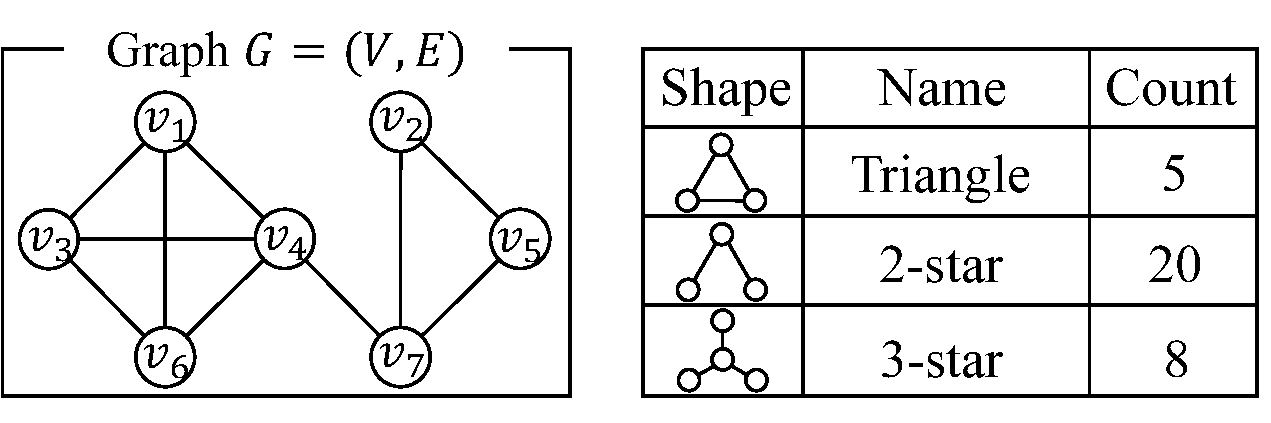
\includegraphics[width=0.9\linewidth]{fig/subgraph.pdf}

\caption[Example of subgraph counts.]{Example of subgraph counts.}
\label{chap1-fig:subgraph}
\end{figure}

In this paper, we consider LDP for graph data, and 
% propose solutions 
provide algorithms and theoretical performance guarantees
for calculating graph statistics in this model. 
In particular, we focus on counting triangles and $k$-stars -- the most basic and useful subgraphs. 
% such as triangles and $k$-stars. 
A triangle is a set of three nodes with three edges (we exclude automorphisms; i.e., \#closed triplets $= 3 \times$ \#triangles). 
A $k$-star consists of a central node connected to $k$ other nodes. 
Figure~\ref{chap1-fig:subgraph} shows an example of triangles and $k$-stars. 
Counting them is a fundamental task of analyzing the connection patterns in a graph, as 
% measures of centrality such as 
the clustering coefficient can be calculated from triangle and $2$-star counts as: $\frac{3 \times \text{\#triangles}}{\#2\text{-stars}}$ (in Figure~\ref{chap1-fig:subgraph}, $\frac{3 \times 5}{20} = 0.75$). 

When we look to protect privacy of relationship information modeled by edges in a graph, 
we need to pay attention to the fact 
% Note 
that some relationship information 
% about friendship (edges) 
could be leaked from subgraph counts. 
For example, 
% consider an adversary who 
suppose that user (node) $v_2$ in Figure~\ref{chap1-fig:subgraph} knows 
all edges connected to $v_2$ and 
all edges between $v_3, \ldots, v_7$ 
as background knowledge, and that $v_2$ wants to know who are friends with $v_1$. 
Then ``\#2-stars = 20'' reveals 
% to $v_2$ 
the fact that $v_1$ has three friends, and ``\#triangles = 5'' reveals 
% to $v_2$ 
the fact that the three friends of $v_1$ are $v_3$, $v_4$, and $v_6$. 
Moreover, a central server that holds all friendship information (i.e., all edges) may face data breaches, as explained above. 
Therefore, a private algorithm for counting subgraphs in the local model is highly beneficial to individual privacy.

%Counting subgraphs in the local model is very challenging. 
The main challenge in counting subgraphs in the local model is that existing techniques and their analysis do not directly apply. 
The existing work on LDP for tabular data assumes that 
each person's data 
is independently and identically drawn from an underlying distribution. 
% (see Section~\ref{chap1-sec:related}). 
In graphs, this is no longer the case; e.g., 
each triangle is not independent, 
because multiple triangles can involve the same edge; 
each $k$-star is not independent for the same reason. 
Moreover, complex inter-dependencies involving multiple people 
% is 
are 
possible in graphs. 
For example, each user cannot count triangles involving herself, because she cannot see edges between other users; 
e.g., 
% in Figure~\ref{chap1-fig:subgraph}, 
user 
% (node) 
$v_1$ cannot see an edge between $v_3$ and $v_4$ in Figure~\ref{chap1-fig:subgraph}. 

% This simultaneously presents both challenges and opportunities. 
We show that although these complex dependency among users introduces challenges, it also presents opportunities. Specifically, this kind of interdependency also implies that extra interaction between users and a data collector may be helpful depending on the prior responses. 
In this work, we investigate this issue and provide algorithms for accurately calculating subgraph counts under LDP. 
% counts that use various levels of interaction. 

\smallskip
\noindent{\textbf{Our contributions.}}~~In this paper, we provide 
% To our knowledge, we are the first to provide 
algorithms and corresponding performance guarantees for counting triangles and $k$-stars in graphs under edge Local Differential Privacy. Specifically, our contributions are as follows:
\begin{itemize}
    \item For triangles, we present two algorithms. The first is based on 
    Warner's RR (Randomized Response) \cite{Warner_JASA65} 
    and empirical estimation \cite{Kairouz_ICML16,Murakami_USENIX19,Wang_USENIX17}. 
    We then present a more sophisticated algorithm that uses an additional round of interaction between users and data collector. We provide upper-bounds on the estimation error for each algorithm, and show that the latter can  significantly reduce the estimation error. 
    
    \item For $k$-stars, we present a simple algorithm using the Laplacian mechanism. We analyze the upper-bound on the estimation error for this algorithm, and 
    show that it is order optimal in terms of the number of users among all LDP mechanisms that do not use additional interaction.
    
    \item We provide lower-bounds on the estimation error for 
    %estimating 
    general graph functions including triangle counts and $k$-star counts in the local model. These are stronger than known upper bounds in the centralized model, and illustrate the limitations of the local model over the central.
    
    \item Finally, we evaluate our algorithms on two real datasets, and show that 
    it is indeed possible to accurately estimate 
    subgraph counts in the local model. 
    %Our experimental results show that 
    %although the algorithms in the local model provide high estimation errors than those in the centralized model,  
    In particular, we show that 
    the interactive algorithm for triangle counts and the Laplacian algorithm for the $k$-stars provide small estimation errors when the number of users is large.
\end{itemize}

We implemented our algorithms with C/C++, and published them as open-source software \cite{LDPGraphStatistics}.

% \smallskip
% \noindent{\textbf{Related work.}}~~Here we explain the previous work related ours. 

%-------------------------------------------------------------------------------
\section{Related Work}
\label{sec:related}
%-------------------------------------------------------------------------------
% Here we review the prior work related to ours. 
% Here we review the previous work on graph DP (Differential Privacy), LDP (Local DP), and upper/lower-bounds.

\smallskip
\noindent{\textbf{Graph DP.}}~~DP on graphs has been widely studied, with most prior work being in the centralized model \cite{blocki2012johnson,Chen_PoPETs20,Day_SIGMOD16,Hay_ICDM09,Karwa_PVLDB11,Kasiviswanathan_TCC13,Nissim_STOC07,Raskhodnikova_arXiv15,Raskhodnikova_Encyclopedia16,Song_arXiv18,Wang_PAKDD13,Wang_TDP13}. 
% Some studies proposed algorithms for counting subgraphs in this model. 
% For example, Karwa \textit{et al.} \cite{Karwa_PVLDB11} proposed an algorithm for counting triangles and $k$-stars by adding the Cauchy noise to the true count. 
% Day \textit{et al.} \cite{Day_SIGMOD16} ...
% Kasiviswanathan \textit{et al.} \cite{Kasiviswanathan_TCC13} 
In this model, a number of algorithms have been proposed for releasing subgraph counts \cite{Karwa_PVLDB11,Kasiviswanathan_TCC13,Song_arXiv18}, degree distributions \cite{Day_SIGMOD16,Hay_ICDM09,Raskhodnikova_arXiv15}, eigenvalues and eigenvectors 
\cite{Wang_PAKDD13}, and synthetic graphs \cite{Chen_PoPETs20,Wang_TDP13}. 

% Algorithms for graph DP in the local model are much fewer, and \cite{Qin_CCS17,Ye_ICDE20,Zhang_USENIX20} are such examples. 
% Some studies proposed 
There has also been a handful of work on graph algorithms in the local DP model~\cite{Qin_CCS17,Sun_CCS19,Ye_ICDE20,Ye_TKDE21,Zhang_USENIX20}. 
For example, Qin \textit{et al.} \cite{Qin_CCS17} propose an algorithm for generating synthetic graphs. 
% while
% Ye \textit{et al.} \cite{Ye_ICDE20} 
% provide a method
% for graph metric estimation under LDP. 
% that perturbs 
% a neighbor list 
% an adjacency matrix by the RR (Randomized Response) 
% and each user's degree by the Laplacian noise. 
Zhang \textit{et al.} \cite{Zhang_USENIX20} propose an algorithm for software usage analysis under LDP, where a node represents a software component (e.g., function in a code) and an edge represents a control-flow between components. 
% None of these works focus on subgraph counts. 
Neither of these works focus on subgraph counts. 

Sun \textit{et al.} \cite{Sun_CCS19} propose an algorithm for counting subgraphs in the local model under the assumption that each user allows her friends to see all her connections. 
However, this assumption does not hold in many practical scenarios; e.g., a Facebook user can change her setting so that friends cannot see her connections. Therefore, we assume that each user knows only her friends rather than all of her friends' friends. 
The algorithms in \cite{Sun_CCS19} cannot be applied to this setting.

Ye \textit{et al.} \cite{Ye_ICDE20} propose a one-round algorithm for estimating graph metrics including the clustering coefficient. 
Here they apply Warner's RR (Randomized Response) to an adjacency matrix. 
However, it introduces a very large bias for triangle counts.
In \cite{Ye_TKDE21}, they propose a method for reducing the bias in the estimate of triangle counts. 
However, the method in \cite{Ye_TKDE21} introduces some approximation, and it is unclear whether their estimate is unbiased. 
In this paper, we propose a one-round algorithm for triangles that uses empirical estimation as a post-processing step, and prove that our estimate is unbiased. 
We also show in Appendix~\ref{sec:RR_emp} that our one-round algorithm significantly outperforms the one-round algorithm in \cite{Ye_ICDE20}. 
Moreover, we show in Section~\ref{sec:experiments} that our two-rounds algorithm significantly outperforms our one-round algorithm.

Our work also differs from \cite{Sun_CCS19,Ye_ICDE20,Ye_TKDE21} in that we provide lower-bounds on the estimation error.

% Our work differs from these in two ways: (i) our work provides algorithms and theoretical performance guarantees for subgraph counts, 
% (ii) we also 
% \colorB{provide} 
% lower-bounds on the estimation error. 
% We note that although Warner's RR (Randomized Response) has been applied to an adjacency matrix in \cite{Qin_CCS17,Ye_ICDE20} for different purposes than ours, it can be used for counting triangles. 
% However, it suffers from a very large estimation error. 
% Our one-round algorithm for triangles uses empirical estimation as a post-processing step, and we show in Appendix~\ref{sec:RR_emp} that this empirical estimation step significantly reduces the estimation error.

\smallskip
\noindent{\textbf{LDP.}}~~Apart from graphs, a number of works have looked at analyzing statistics (e.g., discrete distribution estimation\cite{Acharya_AISTATS19,Fanti_PoPETs16,Kairouz_ICML16,Kairouz_JMLR16,Murakami_USENIX19,Wang_USENIX17,Ye_ISIT17}, 
% and 
heavy hitters \cite{Bassily_STOC15,Bassily_NIPS17,Qin_CCS16}) under LDP. 
% Warner's RR \cite{Warner_JASA65}, $k$-ary RR \cite{Kairouz_ICML16}, RAPPOR \cite{Erlingsson_CCS14}, ...

However, they use LDP in the context of tabular data, and do not consider the kind of complex interdependency in graph data (as described in Section~\ref{sec:intro}). 
% it can happen that their algorithms do not work well for graph data which have complex interdependency. 
For example, the RR with empirical estimation is optimal in the low privacy regimes for estimating a distribution for tabular data \cite{Kairouz_ICML16,Kairouz_JMLR16}. 
We apply the RR and empirical estimation to counting triangles, and show that it is suboptimal and significantly outperformed by a more sophisticated 
two-rounds 
algorithm. 
% with more interaction between users and a data collector. 
% This example shows that directly applying existing LDP techniques does not work well. 

\smallskip
\noindent{\textbf{Upper/lower-bounds.}}~~Finally, we note that existing work on upper-bounds and lower-bounds cannot be directly applied to our setting. 
For example, there are upper-bounds
\cite{Acharya_AISTATS19,Kairouz_ICML16,Kairouz_JMLR16,Ye_ISIT17,Joseph_ArXiv19,Joseph_ArXiv19_Gauss} and
lower-bounds
\cite{Acharya_arXiv20,Duchi_ArXiv14,Duchi_ArXiv17,Joseph_ArXiv19,Duchi_ArXiv19,
Joseph_ArXiv19_Gauss, Joseph_SODA20} on the estimation error (or sample complexity) in 
% estimating a discrete distribution on personal data. 
distribution estimation of tabular data. 
% can be found in \cite{Acharya_AISTATS19,Duchi_ArXiv14,Kairouz_ICML16,Kairouz_JMLR16,Ye_ISIT17}. 
However, they assume that each original data value is independently sampled from an underlying distribution. 
They cannot be directly applied to our graph setting, because each triangle and each $k$-star involve multiple edges and are not independent (as described in Section~\ref{sec:intro}). 
% Acharya \textit{et al.} \cite{Acharya_arXiv20} provides lower-bounds on ...
Rashtchian \textit{et al.} \cite{Rashtchian_arXiv20} provide lower-bounds on communication complexity (i.e., number of queries) of vector-matrix-vector queries for estimating subgraph counts. 
However, their lower-bounds are not on the estimation error, and cannot be applied to our problem.

 %-------------------------------------------------------------------------------
\section{Preliminaries}
%-------------------------------------------------------------------------------
\label{chap1-sec:preliminaries}

% \subsection{Notations and Graphs}
% \label{chap1-sub:notations}
% \subsection{Graphs and Centralized Differential Privacy}
\subsection{Graphs and Differential Privacy}
\label{chap1-sub:graphs_CDP}
\noindent{\textbf{Graphs.}}~~Let $\nats$, $\nnints$, $\reals$, and $\nnreals$ be the sets of natural numbers, non-negative integers, real numbers, and non-negative real numbers, respectively. 
For $a \in \nats$, let $[a] = \{1, 2, \ldots, a\}$. 

We consider an undirected graph $G=(V,E)$, where 
$V$ is a set of nodes (i.e., users) and $E$ is a set of edges. 
Let $n \in \nats$ be the number of users in $V$, and let $v_i \in V$ the $i$-th user; i.e., $V=\{v_1,\ldots,v_n\}$. 
An edge $(v_i, v_j) \in E$ represents a relationship between users $v_i \in V$ and $v_j \in V$. 
% a node $v \in V$ represents a user and an edge $(u,v) \in E$ represents a relationship
% between users $u \in V$ and $v \in V$. 
The number of edges connected to a single node is called the \textit{degree} of the node. 
Let $d_{max} \in \nats$ be the \textit{maximum degree} (i.e., maximum number of edges connected to a node) in graph $G$. 
Let $\calG$ be the set of possible graphs 
% $G=(V,E)$ with $V=\{v_1,\ldots,v_n\}$. 
$G$ on $n$ users. 
A graph $G \in \calG$ can be represented as a symmetric adjacency matrix $\bmA=(a_{i,j}) \in \{0,1\}^{n \times n}$, where $a_{i,j}=1$ if $(v_i,v_j) \in E$ and $a_{i,j}=0$ otherwise.

% \subsection{Centralized Differential Privacy}
% \label{chap1-sub:CDP}
\smallskip
% \noindent{\textbf{Centralized DP.}}~~
\noindent{\textbf{Types of DP.}}~~
DP (Differential Privacy) \cite{DP,Dwork_ICALP06} is known as a gold standard for data privacy. 
According to the underlying architecture, DP can be divided into two 
% categories: 
types: 
\textit{centralized DP} and \textit{LDP (Local DP)}. 
% the one in the centralized (or global) model and the one in the local model. 
% In the centralized model, a trusted database 
Centralized DP assumes the centralized model, where a ``trusted'' data collector 
% database administrator 
collects the original personal data from all users and obfuscates a query (e.g., counting query, histogram query) on the set of personal data. 
% In contrast, 
LDP assumes the local model, where each user does not trust even the data collector. 
In this model, each user obfuscates a query on her personal data by herself and sends the obfuscated data to the data collector. 
% We begin by explaining centralized DP on graphs.

% There are two types of DP on graphs: 
If the data are represented as a graph, we can consider two types of DP: 
% centralized DP: 
% If the input is a graph, we can consider two types of DP: 
% centralized DP: 
% \textit{edge centralized DP} and \textit{node centralized DP} \cite{Hay_ICDM09}. 
\textit{edge DP} and \textit{node DP} \cite{Hay_ICDM09,Raskhodnikova_Encyclopedia16}. 
% We refer to edge DP and node DP in the centralized model as edge centralized DP and node centralized DP, respectively. 
Edge DP considers two neighboring graphs $G, G' \in \calG$ that differ in one edge. 
In contrast, node DP considers two neighboring graphs $G, G' \in \calG$ in which $G'$ is obtained from $G$ by adding or removing one node along with its adjacent edges. 
% Although node DP guarantees stronger privacy than edge DP, 
% it is much harder to attain. 

% Zhang \textit{et al.} \cite{Zhang_USENIX20} proposed an algorithm for software usage analysis with node DP in the local model, where a node represents a software component 
% and an edge represents a control-flow between components. 
% However, we consider a totally different problem, where each node represents a user (rather than a software component). 
Although Zhang \textit{et al.} \cite{Zhang_USENIX20} consider node DP in the local model where each node represents a software component, we consider a totally different problem where each node represents a user. 
% (rather than a software component). 
In the latter case, 
% achieving node DP in the local model is extremely difficult 
% because each user needs to hide the \textit{existence of herself} along with her all edges against the data collector. 
node DP requires us to hide the \textit{existence of each user} along with her all edges. 
% against the data collector. 
However, many applications in the local model send the identity of each user to a server. 
For example, 
we can consider a mobile application 
% that asks a users how many friends she met today and sends noisy counts and her user ID to a server. 
that sends to a server how many friends a user met today along with her user ID. 
In this case, the user may not mind sending her user ID, 
% (i.e., who the user is), 
but may want to hide her edge information (i.e., who she met today). 
Although we cannot use node DP in such applications, we can use edge DP to deny the presence/absence of each edge (friend). 
Thus we focus on edge DP in the same way as \cite{qin2017generating,Sun_CCS19,Ye_ICDE20,Ye_TKDE21}. 

% We refer to edge DP in the centralized model as \textit{edge centralized DP}, and explain it in detail below.
Below we explain edge DP in the centralized model. 

\smallskip
\noindent{\textbf{Centralized DP.}}~~We call edge DP in the centralized model \textit{edge centralized DP}. 
% Edge centralized DP is 
% Edge centralized DP considers two neighboring graphs that differ in one edge. 
Formally, it is defined as follows:

\begin{definition} [$\epsilon$-edge centralized DP] \label{chap1-def:edge_CDP} 
Let $\epsilon \in \nnreals$. 
A randomized algorithm $\calM$ with domain $\calG$ provides \emph{$\epsilon$-edge centralized DP} 
if for any two 
neighboring 
graphs $G, G' \in \calG$ that differ in one edge and any $S \subseteq \mathrm{Range}(\calM)$, 
\begin{align}
\Pr[\calM(G) \in S] \leq e^\epsilon \Pr[\calM(G') \in S].
\label{chap1-eq:edge_CDP}
\end{align}
\end{definition}
Edge centralized DP guarantees that an adversary who has observed the output of $\calM$ cannot determine whether it is come from $G$ or $G'$ with a certain degree of confidence. 
The parameter $\epsilon$ is called the \textit{privacy budget}. 
% and controls the amount of information leaked from the output of $\calM$. 
If $\epsilon$ is close to zero, then $G$ and $G'$ are almost equally likely, which means that an edge in $G$ is strongly protected. 

We also note that edge DP can be 
% easily extended 
used 
to protect $k\in\nats$ edges by using 
the notion of group privacy \cite{DP}.
Specifically, if $\calM$ provides $\epsilon$-edge centralized DP, then for any two graphs $G, G' \in \calG$ that differ in $k$ edges and any $S \subseteq \mathrm{Range}(\calM)$, we obtain: 
$\Pr[\calM(G) \in S] \leq e^{k\epsilon} \Pr[\calM(G') \in S]$; i.e., $k$ edges are protected with privacy budget $k\epsilon$.

\subsection{Local Differential Privacy}
\label{chap1-sub:LDP}
LDP (Local Differential Privacy) \cite{Kasiviswanathan_FOCS08,Duchi_FOCS13} is a privacy metric to protect personal data of each user in the local model. 
LDP has been originally introduced to protect each user's data record that is independent from the other records. 
However, in a graph, each edge is connected to two users. 
Thus, when we define edge DP in the local model, 
% i.e., \textit{edge LDP}, 
we should consider what we want to protect. 
In this paper, we consider two definitions of edge DP in the local model: \textit{edge LDP} in \cite{qin2017generating} and 
% \textit{entire edge LDP} 
\textit{relationship DP} 
introduced in this paper. 
Below, we will explain these two definitions in detail. 

% Applying LDP to a graph is not straightforward 
% because adding or removing one edge will affect neighbor lists of two users. 

\smallskip
\noindent{\textbf{Edge LDP.}}~~Qin \textit{et al.} \cite{qin2017generating} defined edge LDP based on a user's \textit{neighbor list}. 
% use the definition of edge LDP in \cite{qin2017generating}, which is based on a user's \textit{neighbor list}. 
Specifically, 
% given a user in $V$, 
% let $b_i \in \{0,1\}$ be a binary bit that takes $1$ if there is an edge between the user and user $v_i \in V$ and $0$ otherwise. 
% Let 
% $\bmb = (b_1, \ldots, b_n) \in \{0,1\}^n$ be a neighbor list. 
% Let $\bma_i = (a_{i,1}, \ldots, a_{i,n}) \in \{0,1\}^n$ be the $i$-th row of the adjacency matrix $\bmA$. 
% Note that a graph $G$ can be represented as neighbor lists $\textbf{a}_1, \ldots, \textbf{a}_n$, and $\bma_i$ is a neighbor list of user $v_i$. 
let $\bma_i = (a_{i,1}, \ldots, a_{i,n}) \in \{0,1\}^n$ be a neighbor list of user $v_i$. 
Note that $\bma_i$ is the $i$-th row of the adjacency matrix $\bmA$ of graph $G$. 
In other words, graph $G$ can be represented as neighbor lists $\textbf{a}_1, \ldots, \textbf{a}_n$. 

Then edge LDP is defined as follows: 

\begin{definition} [$\epsilon$-edge LDP \cite{qin2017generating}] \label{chap1-def:edge_LDP} 
Let $\epsilon \in \nnreals$. 
For any $i \in [n]$, let $\calR_i$ with domain $\{0,1\}^n$ be a randomized algorithm of user $v_i$. 
% A randomized algorithm $\calR$ with domain $\{0,1\}^n$ 
$\calR_i$ 
provides \emph{$\epsilon$-edge LDP} 
if for any two neighbor lists 
% $\bmb, \bmb' \in \{0,1\}^n$ 
$\bma_i, \bma'_i \in \{0,1\}^n$ 
that differ in one bit and any 
% $S \subseteq \mathrm{Range}(\calR)$, 
$S \subseteq \mathrm{Range}(\calR_i)$, 
\begin{align}
% \Pr[\calR(\bmb) \in S] \leq e^\epsilon \Pr[\calR(\bmb') \in S].
\Pr[\calR_i(\bma_i) \in S] \leq e^\epsilon \Pr[\calR_i(\bma'_i) \in S].
\label{chap1-eq:edge_LDP}
\end{align}
\end{definition}
Edge LDP in Definition~\ref{chap1-def:edge_LDP} protects 
a single bit in a neighbor list with privacy budget $\epsilon$. 
% For example, consider an application that asks a users how many friends she met today and sends noisy counts and her user ID to a server. 
% In this case, the user would not mind sending her identity 
% % (i.e., who the user is), 
% but want to hide who she met today (i.e., who are her neighbors). 
% Edge LDP can be used to deny the presence/absence of one neighbor.
As with edge centralized DP, edge LDP can also be 
% extended 
used 
to protect $k \in \nats$ 
bits in a neighbor list 
% neighbors 
by using group privacy; i.e., $k$ bits in a neighbor list are protected with privacy budget $k\epsilon$. 

% We can consider an application of the randomized algorithm $\calR$ with input $\bmb$ as follows. 
% For example, suppose that a data collector asks each user to send some query (e.g., number of friends, who are friends) on her neighbor list $\bmb$. 
% To protect $\bmb$, each user obfuscates her answer to the query by using $\calR$ and sends the noisy answer to the data collector. 
% Then the data collector estimates some graph statistics 
% (e.g., number of triangles, clustering coefficient) 
% based on the noisy answer from each user. 

\smallskip
% \noindent{\textbf{RNL (Randomized Neighbor List).}}~~
\noindent{\textbf{RR (Randomized Response).}}~~As a simple example of a randomized algorithm 
% $\calR$ 
$\calR_i$ 
providing $\epsilon$-edge LDP, we explain 
% the 
Warner's RR (Randomized Response) \cite{Warner_JASA65} applied to a neighbor list, 
which is called 
% the RNL (Randomized neighbor List) 
the randomized neighbor list in \cite{qin2017generating}. 
% and is also used in \cite{Ye_ICDE20}. 

Given a neighbor list 
% $\bmb \in \{0,1\}^n$, 
$\bma_i \in \{0,1\}^n$, 
% the RNL 
this algorithm 
outputs a noisy neighbor lists 
% $\bms = (s_1, \ldots, s_n) \in \{0,1\}^n$ 
$\bmb = (b_1, \ldots, b_n) \in \{0,1\}^n$ 
by flipping each bit in 
% $\bmb$ 
$\bma_i$ 
with probability $p = \frac{1}{e^\epsilon + 1}$; i.e., for each $j \in [n]$, 
% $s_i \neq b_i$ with probability $p$ and $s_i = b_i$ with probability $1-p$. 
$b_j \neq a_{i,j}$ with probability $p$ and $b_j = a_{i,j}$ with probability $1-p$. 
Since 
% $\Pr[\calR(\bmb) \in S]$ and $\Pr[\calR(\bmb') \in S]$ 
$\Pr[\calR(\bma_i) \in S]$ and $\Pr[\calR(\bma'_i) \in S]$ 
in (\ref{chap1-eq:edge_LDP}) differ by $e^\epsilon$ for 
% $\bmb$ and $\bmb'$ 
$\bma_i$ and $\bma'_i$ 
that differ in one bit, 
% It is easy to verify that 
% the RNL 
this algorithm 
provides $\epsilon$-edge LDP. 

\smallskip
% \noindent{\textbf{Remark.}}~~
% \noindent{\textbf{Alternative definition of edge LDP.}}~~
\noindent{\textbf{Relationship DP.}}~~In graphs such as social networks, 
% For graph datasets, 
it is usually the case that two users share knowledge of the presence of an edge between them. 
% For example, in social networks it is usually the norm that
% friendship status is known by both parties.
% With the goal of hiding their mutual edge, 
To hide their mutual edge, 
we must consider
that both user's outputs can leak information. 
We introduce a DP definition called relationship DP that hides \textit{one entire edge in graph $G$ during the whole process:}
% avoid confusion. 
% For example, divide a graph $G$ into disjoint sets $(G_1, \ldots, G_n)$ such that user $v_i$ can see $G_i$. 
% For example, 

% Then 
% We define relationship DP as follows: 
% (we call this version of edge LDP \textit{entire edge LDP} to avoid confusion):

\begin{definition} [$\epsilon$-relationship DP] 
% [$\epsilon$-entire edge LDP] 
\label{chap1-def:entire_edge_LDP} 
Let $\epsilon \in \nnreals$. 
% Let $\calR_1, \ldots, \calR_n$ be randomized algorithms, each of which is with domain $\{0,1\}^n$. 
A tuple of randomized algorithms $(\calR_1, \ldots, \calR_n)$, 
each of which is with domain $\{0,1\}^n$, 
provides 
% \emph{$\epsilon$-entire edge LDP} 
\emph{$\epsilon$-relationship DP} 
if for any two 
neighboring 
graphs $G, G' \in \calG$ that differ in one edge and any $S \subseteq \mathrm{Range}(\calR_1) \times \ldots \times \mathrm{Range}(\calR_n)$, 
\begin{align}
&\Pr[(\calR_1(\bma_1), \ldots, \calR_n(\bma_n)) \in S] \nonumber\\
&\leq e^\epsilon \Pr[(\calR_1(\bma'_1), \ldots, \calR_n(\bma'_n)) \in S],
\label{chap1-eq:entire_edge_LDP}
\end{align}
where $\bma_i$ (resp.~$\bma'_i$) $\in \{0,1\}^n$ is the $i$-th row of the adjacency matrix of graph $G$ (resp.~$G'$).
\end{definition}

Relationship DP is the same as \textit{decentralized DP} in \cite{Sun_CCS19} except that the former (resp.~latter) assumes that each user knows only her friends (resp.~all of her friends' friends).

% Relationship DP is distinct from edge LDP because 
Edge LDP assumes that 
% user $v_i$ being connected to user $v_j$ 
user $v_i$'s edge connected to user $v_j$ 
and 
% user $v_j$ being connected to user $v_i$ 
user $v_j$'s edge connected to user $v_i$ 
are different secrets, with user $v_i$ knowing the former and user $v_j$ knowing the latter. 
% As we stated above, the presence of an edge is usually known by both its users. 
Relationship DP assumes that the two secrets are the same.

% Since secrets are shared among two users, 
Note that 
the threat model of relationship DP is 
% not quite 
different from 
that of 
% local DP: 
LDP -- 
some amount of trust must be given to the other users 
in relationship DP. 
Specifically, user $v_i$ must trust user $v_j$ to not leak information
about their shared edge. If $k \in \nats$ users decide not to follow their protocols, 
then up to $k$ edges incident to user $v_i$ may be compromised. This trust model
is stronger than 
% local DP, 
LDP, 
which assumes nothing about what other users 
% may 
do,
but is much weaker than centralized DP in which 
% all information of a user is 
all edges are 
in the hands of the central party.

Other than the differing threat models, relationship DP and edge LDP are quite closely related:

\begin{proposition} \label{chap1-prop:edge_LDP_entire_edge_LDP} 
If randomized algorithms $\calR_1, \ldots, \calR_n$ provide $\epsilon$-edge LDP, 
then $(\calR_1, \ldots, \calR_n)$ provides $2\epsilon$-relationship DP.
\end{proposition}

\begin{proof}
The existence of edge $(v_i, v_j) \in E$ affects two elements $a_{i,j}, a_{j,i} \in \{0,1\}$ in the adjacency matrix $\bmA$. 
  Then by group privacy~\cite{DP}, Proposition~\ref{chap1-prop:edge_LDP_entire_edge_LDP} holds.
\end{proof}

% The existence of edge $(v_i, v_j) \in E$ affects two elements $a_{i,j}, a_{j,i} \in \{0,1\}$ in the adjacency matrix $\bmA$. 
% Therefore, by the composition theorem \cite{DP}, if all of the randomized algorithms $\calR_1, \ldots, \calR_n$ provide $\epsilon$-edge LDP in Definition~\ref{chap1-def:edge_LDP}, 
% then the tuple $(\calR_1, \ldots, \calR_n)$ provides $2\epsilon$-entire edge LDP in Definition~\ref{chap1-def:entire_edge_LDP}; i.e., the privacy budget is at most doubled. 

Proposition~\ref{chap1-prop:edge_LDP_entire_edge_LDP} states that when we want to protect one edge as a whole, the privacy budget is at most doubled. 
Note, however, that 
% the privacy budget is not changed for some randomized algorithms. 
some randomized algorithms do not have this doubling issue. 
For example, we can apply the RR to the $i$-th neighbor list $\bma_i$ so that $\calR_i$ outputs noisy bits 
% $(t_{i+1}, \ldots, t_n) \in \{0,1\}^{n-i}$ 
% $(t_1, \ldots, t_{i-1}) \in \{0,1\}^{i-1}$ 
$(b_1, \ldots, b_{i-1}) \in \{0,1\}^{i-1}$ 
for only users 
% $v_{i+1}, \ldots, v_n$ with larger user IDs; 
$v_1, \ldots, v_{i-1}$ with smaller user IDs; 
i.e., 
% In other words, we can modify the RNL as follows: 
for each 
% $j \in \{i+1, \ldots, n\}$, 
$j \in \{1, \ldots, i-1\}$, 
% $\calR_i$ outputs $(t_{i+1}, \ldots, t_n) \in \{0,1\}^{n-i}$, where 
% $t_j \neq a_{i,j}$ with probability $p = \frac{1}{e^\epsilon + 1}$ and $t_j = a_{i,j}$ with probability $1-p$. 
$b_j \neq a_{i,j}$ with probability $p = \frac{1}{e^\epsilon + 1}$ and $b_j = a_{i,j}$ with probability $1-p$. 
In other words, we can extend 
% the RNL 
the RR for a neighbor list 
so that $(\calR_1, \ldots, \calR_n)$ outputs only 
% the upper triangular part 
the lower triangular part 
of the noisy adjacency matrix. 
Then all of $\calR_1, \ldots, \calR_n$ provide $\epsilon$-edge LDP. 
In addition, the existence of edge $(v_i, v_j) \in E$ 
% $(i < j)$ 
$(i > j)$ 
affects only one element $a_{i,j}$ in 
% the upper triangular part 
the lower triangular part 
of $\bmA$. 
Thus, $(\calR_1, \ldots, \calR_n)$ provides $\epsilon$-relationship DP (not $2\epsilon$). 
% Note that this extended algorithm requires each user to know who are users with larger user IDs. 
% One way to do so is to send user IDs of $n$ users from the data collector to each user in advance. 

Our proposed algorithm in Section~\ref{chap1-sub:two_rounds} also has this property; i.e., 
it provides both $\epsilon$-edge LDP and $\epsilon$-relationship DP. 
% can also be extended so that the tuple $(\calR_1, \ldots, \calR_n)$ provides $\epsilon$-entire edge LDP (not $2\epsilon$), given that each user knows users with larger user IDs. 
% We describe the extended algorithm in Appendix~\ref{chap1-sec:modified_two_rounds}. 


% \smallskip
% \noindent{\textbf{Global/local sensitivity.}}~~
% \subsection{Global Sensitivity and Local Sensitivity}
\subsection{Global Sensitivity}
\label{chap1-sub:sensitivity}
In this paper, we use the notion of global sensitivity \cite{DP} to provide edge centralized DP or edge LDP.
% In this paper, we use the local sensitivity \cite{Nissim_STOC07} to provide 
% edge centralized DP or edge LDP with small noise.
% Here we explain the global sensitivity \cite{DP} and the local sensitivity \cite{Nissim_STOC07}. 

Let $\calD$ be the set of possible input data of a randomized algorithm. 
In edge centralized DP, $\calD = \calG$. 
In edge LDP, $\calD = \{0,1\}^n$. 
Let $f: \calD \rightarrow \reals$ be a function that takes data $D \in \calD$ as input and outputs some statistics $f(D) \in \reals$ about the data. 
% $f: \calG \rightarrow \reals$ 
% be a function that takes a graph $G \in \calG$ as input and outputs some graph statistics $f(G) \in \reals$. 
% Assume that we want to estimate some graph statistics $f(G) \in \reals$. 
The most basic method for providing DP is to add the Laplacian noise proportional to the global sensitivity \cite{DP}.

\begin{definition} [Global sensitivity] \label{chap1-def:global_sen} 
The global sensitivity of a function $f: \calD \rightarrow \reals$ is given by:
\begin{align*}
GS_f = \underset{D,D' \in \calD: D \sim D'}{\max} |f(D) - f(D')|,
%\label{chap1-eq:global_sen}
\end{align*}
where $D \sim D'$ represents that $D$ and $D'$ are neighbors; i.e., they differ in one edge in edge centralized DP, and differ in one bit in edge LDP.
\end{definition}

% For example, consider a function that 
% takes a neighbor list $\bma_i$ of user $v_i$ and outputs the number of $2$-stars of which she is a center. 
% Since adding 

% For $b \in \nnreals$, let $\Lap(b)$ be a random variable that represents the Laplacian noise with mean $0$ and scale $b$. 
% Then for $\epsilon \in \nnreals$, $f(D) + \Lap(GS_f/\epsilon)$ provides $\epsilon$-DP. 
% Here $\epsilon$-DP can be instantiated by $\epsilon$-edge centralized DP or $\epsilon$-edge LDP. 

% In graph privacy, the global sensitivity $GS_f$ can be very large. 
% since adding one edge in $G$ can result in 
% the increase of $n-2$ triangles, 
% $GS_f = 2 \binom{n}{k-1}$ for $k$-star counts and 
% $GS_f = n-2$ for triangle counts under edge centralized DP. 
% Similarly, the global sensitivity is large for $k$-star counts.
% In practice, the global sensitivity $GS_f$ can be very large. 
In graphs, the global sensitivity $GS_f$ can be very large. 
For example, adding one edge may result in the increase of triangle (resp.~$k$-star) counts by $n-2$ (resp.~$\binom{n}{k-1}$). 

One way to significantly reduce the global sensitivity is to use \textit{graph projection} \cite{Day_SIGMOD16,Kasiviswanathan_TCC13,Raskhodnikova_arXiv15}, which removes some neighbors from a neighbor list so that the maximum degree $d_{max}$ is upper-bounded by a predetermined value $\td_{max} \in \nnints$. 
By using the graph projection with $\td_{max} \ll n$, we can enforce small global sensitivity; e.g., the global sensitivity of triangle (resp.~$k$-star) counts is at most $\td_{max}$ (resp.~$\binom{\td_{max}}{k-1}$) after the projection. 
% This technique is also known as \textit{clipping} \cite{Abadi_CCS16,Thakkar_arXiv19}.
% so that the local sensitivity is upper-bounded by the private estimate of $LS_f(D)$. 

Ideally, we would like to set $\td_{max} = d_{max}$ to avoid removing neighbors from a neighbor list (i.e., to avoid the loss of utility). 
However, the maximum degree $d_{max}$ can leak some information about the original graph $G$. 
In this paper, we address this issue by privately estimating $d_{max}$ with edge LDP and then using the private estimate of $d_{max}$ as $\td_{max}$.
% We call 
This technique 
is also known as 
\textit{adaptive clipping} 
% , and is studied for determining an appropriate threshold of the gradient $l_2$-norm 
% This is also studied for 
in differentially private stochastic gradient descent (SGD) \cite{Pichapati_arXiv19,Thakkar_arXiv19}.


% Nissim \textit{et al.} \cite{Nissim_STOC07} introduced a local measure of sensitivity called the \textit{local sensitivity} to address this issue. 

% \begin{definition} [Local sensitivity \cite{Nissim_STOC07}] \label{chap1-def:local_sen} 
% The local sensitivity of a function $f: \calD \rightarrow \reals$ at $D \in \calD$ is given by:
% \begin{align*}
% LS_f(D) = \underset{D' \in \calD: D \sim D'}{\max} |f(D) - f(D')|.
% \end{align*}
% \end{definition}
% Note that $GS_f = \max_{D \in \calD} LS_f(D)$. 
% In practice, $LS_f(D)$ can be much smaller than $GS_f$. 
% For example, the local sensitivity of triangle counts in $G$ is at most the maximum degree $d_{max}$, which is much smaller than $GS_f = n-2$ when $G$ is sparse. 

% The local sensitivity $LS_f(D)$ cannot be directly used, 
% because the noise magnitude can leak some information about $G$. 
% Karwa \textit{et al.} \cite{Karwa_PVLDB11} showed that in the centralized graph model, adding the Cauchy noise (rather than the Laplacian noise) with the local sensitivity 
% to $k$-star or triangle counts in $G$ provides $\epsilon$-edge centralized DP under some conditions. 
% However, in the local graph model, it is even difficult for users to know the local sensitivity itself. 
% In this paper, we address this issue by privately estimating 
% $LS_f(D)$ 
% with edge LDP and then applying \textit{graph projection} \cite{Day_SIGMOD16,Kasiviswanathan_TCC13,Raskhodnikova_arXiv15}, which removes some neighbors from a neighbor list, 
% so that the local sensitivity is upper-bounded by the private estimate of $LS_f(D)$. 

% if we provide $\epsilon_0$-DP for $LS_f(D)$ by adding noise, adding the noisy $\Lap(LS_f/\epsilon)$ to $f(D)$ provides $(\epsilon_0 + \epsilon)$-DP by the composition theorem \cite{DP}.



\subsection{Graph Statistics and Utility Metrics}
\label{chap1-sub:graph_statistics}

\noindent{\textbf{Graph statistics.}}~~We consider a graph function that takes a graph $G \in \calG$ as input and outputs some graph statistics. 
% Here we consider two types of graph statistics. 
% The first type is \textit{subgraph counts}. 
Specifically, 
let $f_\triangle: \calG \rightarrow \nnints$ be a graph function that outputs the number of triangles in $G$. 
For $k \in \nats$, let $f_{k\star}: \calG \rightarrow \nnints$ be a graph function that outputs the number of $k$-stars in $G$. 
% We call $f_\triangle$ and $f_{k\star}$ the \textit{triangle function} and \textit{$k$-star function}, respectively. 
For example, if a graph $G$ is as shown in Figure~\ref{chap1-fig:subgraph}, then $f_\triangle(G) = 5$, $f_{2\star}(G) = 20$, and $f_{3\star}(G) = 8$. The clustering coefficient can also be calculated from $f_\triangle(G)$ and $f_{2\star}(G)$ as: $\frac{3 f_\triangle(G)}{f_{2\star}(G)} = 0.75$. 

% The second type of graph statistics is \textit{degree information}. 
% For this type of statistics, we define the following basic function. 
% For $i \in [n]$, let $f_{d_i}: \calG \rightarrow \nnints$ be a graph function that 
% outputs a degree (i.e., the number of edges) of user $v_i$ in $G$. 
% We call $f_{d_i}$ the \textit{degree function}. 
% In Figure~\ref{chap1-fig:subgraph}, 
% $f_{d_1}(G) = 3, f_{d_2}(G) = 2, \ldots, f_{d_7}(G) = 3$. 
% A degree distribution can be easily calculated from 
% $f_{d_1}(G), \ldots, f_{d_n}(G)$. 
% In Figure~\ref{chap1-fig:subgraph}, the degree distribution can be expressed as $(0, 0, \frac{2}{7}, \frac{4}{7}, \frac{1}{7})$, where the $i$-th value represents the ratio of $(i-1)$ in 
% $f_{d_1}(G), \ldots, f_{d_n}(G)$; 
% e.g., the 5th value is $\frac{1}{7}$ because ``4'' appears once ($f_{d_4}(G) = 4$). 

% \begin{table}[t]
% \caption{Basic notations in this paper.} 
% \centering
% \hbox to\hsize{\hfil
% \begin{tabular}{l|l}
% \hline
% Symbol		&	Description\\
% \hline
% $G=(V,E)$   &	    Graph with $n$ nodes (users) $V$ and edges $E$\\
% $v_i$       &       $i$-th user in $V$.\\
% $d_{max}$   &       Maximum degree of $G$.\\
% $\calG$     &       Set of possible graphs on $n$ users.\\
% $\bmA$	    &		Adjacency matrix.\\
% $\bma_i$	&		$i$-th row of $\bmA$ (i.e., neighbor list of $v_i$).\\
% $\calR_i$     &       Randomized algorithm on $\bma_i$.\\
% $f_\triangle(G)$   &  Number of triangles in $G$.\\
% $f_{k\star}(G)$    &  Number of $k$-stars in $G$.\\
% \hline
% \end{tabular}
% \hfil}
% \label{chap1-tab:notations}
% \end{table}

\begin{table}[t]
\caption[Basic notations in this paper.]{Basic notations in this paper.} 
\centering
\hbox to\hsize{\hfil
\begin{tabular}{l|l}
\hline
Symbol		&	Description\\
\hline
$n$         &	    Number of users.\\
$G=(V,E)$   &	    Graph with $n$ nodes (users) $V$ and edges $E$.\\
$v_i$       &       $i$-th user in $V$.\\
$d_{max}$   &       Maximum degree of $G$.\\
$\td_{max}$   &       Upper-bound on $d_{max}$ (used for projection).\\
$\calG$     &       Set of possible graphs on $n$ users.\\
$\bmA=(a_{i,j})$	    &		Adjacency matrix.\\
$\bma_i$	&		$i$-th row of $\bmA$ (i.e., neighbor list of $v_i$).\\
$\calR_i$     &       Randomized algorithm on $\bma_i$.\\
$f_\triangle(G)$   &  Number of triangles in $G$.\\
$f_{k\star}(G)$    &  Number of $k$-stars in $G$.\\
\hline
\end{tabular}
\hfil}
\label{chap1-tab:notations}
\end{table}

% \colorB{We show the basic notations in Table~\ref{chap1-tab:notations} of Appendix~\ref{chap1-sec:notations}.} 
Table~\ref{chap1-tab:notations} shows the basic notations used in this paper.

\smallskip
\noindent{\textbf{Utility metrics.}}~~We use the $l_2$ loss (i.e., squared error) \cite{Kairouz_ICML16,Wang_USENIX17,Murakami_USENIX19} and the relative error \cite{Bindschaedler_SP16,Chen_CCS12,Xiao_SIGMOD11} as utility metrics. 

% In our theoretical analysis, we use the $l_2$ loss between the true value and the estimate. 
Specifically, let 
% $\hf: \calG \rightarrow \reals$ be a function that takes a graph $G \in \calG$ as input and outputs an estimate $\hf(G) \in \reals$ of graph statistics $f(G) \in \nnints$.
$\hf(G) \in \reals$ be an estimate of graph statistics $f(G) \in \reals$. 
Here $f$ can be instantiated by 
% $f_\triangle$, $f_{k\star}$, or $f_{d_i}$; 
$f_\triangle$ or $f_{k\star}$; 
i.e., 
% $\hf_\triangle(G)$, $\hf_{k\star}(G)$, and $\hf_{d_i}(G)$ are the estimates of $f_\triangle(G)$, $f_{k\star}(G)$, and $f_{d_i}(G)$, respectively. 
$\hf_\triangle(G)$ and $\hf_{k\star}(G)$ are the estimates of $f_\triangle(G)$ and $f_{k\star}(G)$, respectively. 
Let $l_2^2$ be the $l_2$ loss function, which maps the estimate $\hf(G)$ and the true value $f(G)$ to the $l_2$ loss; i.e., $l_2^2(\hf(G), f(G)) = (\hf(G) - f(G))^2$. 
% \begin{align*}
% l_2^2(\hf(G), f(G)) = (\hf(G) - f(G))^2. 
% \end{align*}
% We denote the estimates of $f_\triangle(G)$, $f_{k\star}(G)$, and $f_{d_i}(G)$ by $\hf_\triangle(G)$, $\hf_{k\star}(G)$, and $\hf_{d_i}(G)$, respectively. 
% When we estimate graph statistics based on the output of 
% 
Note that when we use a randomized algorithm providing edge LDP (or edge centralized DP), $\hf(G)$ depends on the randomness in the algorithm. 
In our theoretical analysis, we analyze the expectation of the $l_2$ loss over 
the randomness, as with \cite{Kairouz_ICML16,Wang_USENIX17,Murakami_USENIX19}. 
% possible realization of $\hf(G)$.
% For 
% and analyze their $l_2$ loss in our theoretical analysis in the same way as . 
% In our experiments, we replace the expectation of the $l_2$ loss with the sample mean of the $l_2$ loss over multiple realizations of 

When $f(G)$ is large, the $l_2$ loss can also be large. 
Thus in our experiments, we also evaluate the relative error, along with the $l_2$ loss. 
The relative error is defined as: $\frac{|\hf(G) - f(G)|}{\max\{f(G), \eta\}}$, where $\eta \in \nnreals$ is a very small positive value. 
Following the convention \cite{Bindschaedler_SP16,Chen_CCS12,Xiao_SIGMOD11}, we set $\eta = 0.001n$ 
for $f_\triangle$ and $f_{k\star}$. 
% Ideally, the relative error should be small than $1$.

%-------------------------------------------------------------------------------
\section{Algorithms}
\label{chap1-sec:algorithms}
%-------------------------------------------------------------------------------
% When the data collector does not have access to the adjacency matrix
% $\bmA$, a unique communication challenge arises. 
In the local model, 
% There 
there 
are several ways 
% in which we may 
to 
model how the data collector interacts with 
the users~\cite{Duchi_FOCS13,Joseph_SODA20,Qin_CCS17}.
The simplest model 
would be 
% is 
to assume that 
% \colorB{each user $v_i$ independently runs the randomized algorithm $\calR_i$ on the neighbor list $\bma_i$ and sends the output $\calR_i(\bma_i)$ to the data collector.} 
the data collector sends 
% one 
a 
query $\calR_i$ to each user $v_i$ once, 
and then 
% and no communication among users occurs.
% The data collector would then receive 
% receives an answer $\calR_i(\bma_i)$ from each user $v_i$. 
each user $v_i$ independently sends an answer $\calR_i(\bma_i)$ to the data collector. 
% independent copies of the random variables
% $(\calR_1(\bma_1), \ldots, \calR_n(\bma_n))$. 
In this model, there is one-round interaction between each user and the data collector. 
We call this the
% \textit{non-interactive graph LDP model}. 
\textit{one-round LDP model}. 
% This model is also called the \textit{non-interactive model}~\cite{Duchi_FOCS13,Joseph_SODA20} because there is no interaction among users (note that there is interaction between each user and the data collector). 
For example, the RR 
%(Randomized Response) 
for a neighbor list in Section~\ref{chap1-sub:LDP} assumes this model.

However, in certain cases it may be possible 
for the data collector to send a query to each user multiple times. 
This could allow for more powerful queries that result in more accurate 
% analysis of graph statistics 
subgraph counts 
\cite{Sun_CCS19} 
or more accurate synthetic graphs~\cite{Qin_CCS17}. 
We call this the \textit{multiple-rounds LDP model}. 
% For example, a synthetic graph generation technique in the two-rounds LDP model has been proposed in~\cite{Qin_CCS17}.

% Note that we assume interaction between each user and the data collector, and do not assume interaction among users in both the one-round and multiple-rounds LDP models.}

% to ask user $i$ an interactive
% query $\calR_i$; namely, it may
% depend on $(\calR_1(\bma_1), \ldots, \calR_{i-1}(\bma_{i-1}))$.
% This could allow for more powerful queries, but the drawback compared to the
% non-interactive graph LDP model
% is that the data collector must wait for user $i-1$ to 
% respond before querying user $i$. We still assume the data collector queries each user
% once, albeit in an arbitrary order. 
% This is the \textit{sequentially interactive graph
% LDP model}.
% 
% These models have been studied before in local differential
% privacy~\cite{Joseph_SODA20}, but not in the graph setting. 
% There is an additional, \textit{fully interactive} model~\cite{Joseph_SODA20} 
% where users may be queried interactively in any order.
% Our algorithms and theorems do not involve this model, and analyzing this
% model in the graph setting is left as future work.

In 
% Section~\ref{chap1-sub:one_round}, 
Sections~\ref{chap1-sub:non-interactive_k_stars} and \ref{chap1-sub:non-interactive_triangles}, 
we consider the problems of computing $f_{k\star}(G)$ 
and $f_\triangle(G)$ 
for a graph $G \in \calG$ in the 
% non-interactive graph 
one-round 
LDP model. 
% These problems are simple but are commonly used to understand the structure of $G$. 
% The algorithms and bounds we have also 
Our algorithms and bounds highlight limitations of the
% non-interactive graph 
one-round 
LDP model. Compared to the centralized graph DP model, the
% non-interactive graph 
one-round 
LDP model cannot compute $f_{k\star}(G)$ as accurately.
Furthermore, the algorithm for $f_\triangle(G)$ does not perform 
well. 
% as well as the
% sequentially-interactive graph 
% two-rounds LDP algorithm, as we will see in
% Section~\ref{chap1-sub:two_rounds}. 
% we consider some algorithms for computing the numbers of $k$-stars $f_{k\star}(G)$ and triangles $f_\triangle(G)$ for a graph $G \in \calG$ in the one-round LDP model, and analyze their expected $l_2$ loss. 
% We also show lower bounds on the expected $l_2$ loss in this model. 
In Section~\ref{chap1-sub:two_rounds}, we propose a more sophisticated algorithm for computing  $f_\triangle(G)$ in the two-rounds LDP model, and show that it provides much smaller expected $l_2$ loss than the algorithm in the one-round LDP model.
In Section~\ref{chap1-sub:lower_bounds}, we show a general result about lower bounds on the expected $l_2$ loss of graph statistics in LDP. 
The proofs of all statements in Section~\ref{chap1-sec:algorithms} are given in 
\conference{the full version \cite{Imola_arXiv21}}\arxiv{Appendix~\ref{chap1-sec:proof}}.

% \subsection{One-Round LDP Algorithms for $k$-Stars}
\subsection{One-Round Algorithms for $k$-Stars}
\label{chap1-sub:non-interactive_k_stars}
% \colorB{Non-interactive Graph LDP Algorithms}}
% \label{chap1-sub:one_round}

% \smallskip
% \noindent{\textbf{\colorB{Non-interactive algorithm for $k$-stars.}}}~~
% \subsubsection{\colorB{One-round LDP algorithm for $k$-stars.}}
% \label{chap1-subsub:non-interactive_k_stars}
\noindent{\textbf{Algorithm.}}~~We begin with the problem of computing $f_{k\star}(G)$ in the 
% non-interactive graph 
one-round 
LDP model. 
For this model, we introduce a simple algorithm using the Laplacian mechanism, and prove that this algorithm can achieve order optimal expected $l_2$ loss among all one-round LDP algorithms. 

\setlength{\algomargin}{4mm}
\begin{algorithm}
  \SetAlgoLined
  \KwData{Graph $G$ 
  %described by distributed 
  represented as 
  neighbor lists $\bma_1, \ldots, \bma_n \allowbreak \in \{0,1\}^n$, privacy budget $\epsilon \in \nnreals$, $\td_{max} \in \nnints$.}
  %$d_{max}$, $k$.}
  \KwResult{Private estimate of $f_{k\star}(G)$.}
  %\colorB{$\texttt{GraphProjection}(\bma_1, \ldots, \bma_n, \td_{max})$\;}
  %$(\bma_1, \ldots, \bma_n) \leftarrow \texttt{GraphProjection}(\bma_1, \ldots, \bma_n)$\;
  %$\Delta \leftarrow \binom{d_{max}}{k-1}$\;
  $\Delta \leftarrow \binom{\td_{max}}{k-1}$\;
  \For{$i=1$ \KwTo $n$}{
    $\bma_i \leftarrow \texttt{GraphProjection}(\bma_i, \td_{max})$\;
    \tcc{$d_i$ is a degree of user $v_i$.}
    %\tcc{degree of vertex $i$.}
    %$d_i \leftarrow \sum_{j=1}^n a_i^j$\;
    $d_i \leftarrow \sum_{j=1}^n a_{i,j}$\;
    %\colorB{\If{$d_i > \td_{max}$}{$d_i = \td_{max}$\;}}
    $r_i \leftarrow \binom{d_i}{k}$\;
    $\hat{r}_i \leftarrow r_i + \Lap\left(\frac{\Delta}{\epsilon}\right)$\;
    $release(\hat{r}_i)$\;
  }
  \KwRet{$\sum_{i=1}^n \hat{r}_i$}
%   \caption{CountKStars\label{chap1-alg:k-stars}}
  \caption{\alg{LocalLap$_{k\star}$}\label{chap1-alg:k-stars}}
\end{algorithm}

Algorithm~\ref{chap1-alg:k-stars} shows the one-round algorithm for $k$-stars. 
It takes as input a graph $G$ (represented as neighbor lists $\bma_1, \ldots, \bma_n \in \{0,1\}^n$), the privacy budget $\epsilon$, and a non-negative integer $\td_{max} \in \nnints$. 
% such that $\td_{max} \geq d_{max}$. 
% $\td_{max}$ is an upper-bound on the maximum degree $d_{max}$ of $G$. 
% If $d_{max} > \td_{max}$, we perform graph projection \cite{Day_SIGMOD16,Raskhodnikova_arXiv15}, as we describe in detail below). 

The parameter $\td_{max}$ plays a role as an upper-bound on the maximum degree $d_{max}$ of $G$. 
Specifically, let $d_i \in \nnints$ be the degree of user $v_i$; i.e., the number of ``$1$''s in her neighbor list $\bma_i$. 
% If $d_i > d_{max}$, we set $d_i = d_{max}$ (lines 4 to 6). 
% In other words, we perform graph projection, which removes some neighbors from a neighbor list so that each user's degree does not exceed $\td_{max}$. 
In line 3, user $v_i$
uses a function (denoted by \texttt{GraphProjection}) that performs graph projection \cite{Day_SIGMOD16,Kasiviswanathan_TCC13,Raskhodnikova_arXiv15} for $\bma_i$ as follows. 
% so that $d_i$ does not exceed $\td_{max}$ as follows. 
If $d_i$ exceeds $\td_{max}$, it randomly 
selects $\td_{max}$ neighbors out of $d_i$ neighbors; otherwise, it uses $\bma_i$ as it is. 
% generates a permutation of $1,\ldots,n$ (the random seed can be different from user to user). 
% Then it selects $\hd_{max}$ neighbors from her neighbor list $\bma_i$ in the order of the permutation.
% user $v_i$ randomly selects $\hd_{max}$ neighbors from her neighbor list $\bma_i$ (otherwise, user $v_i$ uses $\bma_i$ as it is). 
% For example, if $n=6$, $\bma_1=(0,1,0,1,1,1)$, $\td_{max}=3$, and the permutation is $2,3,4,1,6,5$, then 
% it selects the second, fourth, and sixth users; i.e., $\bma_1$ becomes $\bma_1=(0,1,0,1,0,1)$ after the graph projection. 
This guarantees that each user's degree never exceeds $\td_{max}$; i.e., $d_i \leq \td_{max}$ after line 4. 

% In Algorithm~\ref{chap1-alg:k-stars}, each user $v_i$ has her neighbor list $\bma_i$. 
% Based on $\bma_i$, 
% Algorithm~\ref{chap1-alg:k-stars} computes the number of $k$-stars in $G$ with no interaction. Each 
After the graph projection, 
user $v_i$ 
counts the number of $k$-stars $r_i \in \nnints$ of which she is a center (line 5), and 
adds the Laplacian noise 
% with the local sensitivity 
to 
% the number of $k$-stars 
$r_i$ 
(line 6). 
Here, since adding one edge results in the increase of at most $\binom{\td_{max}}{k-1}$ $k$-stars, the 
% local 
% global 
sensitivity of 
% the Laplacian mechanism 
%the $k$-star query 
$k$-star counts for user $v_i$ 
is at most $\binom{\td_{max}}{k-1}$ (after graph projection). 
% Note that if $d_{max}$ is publicly available, then the local sensitivity is also publicly available. 
Therefore, we add $\Lap(\frac{\Delta}{\epsilon})$ to $r_i$, where $\Delta = \binom{\td_{max}}{k-1}$ and 
for $b \in \nnreals$ 
$\Lap(b)$ is a random variable that represents the Laplacian noise with mean $0$ and scale $b$. 
% in Algorithm~\ref{chap1-alg:k-stars}. 
% does the Laplace mechanism using the sensitivity of the $k$-star query which is
% $O(d_{max}^{2k-2})$. 
The final answer of Algorithm~\ref{chap1-alg:k-stars} is
simply the sum of all the noisy $k$-star counts. 
We denote this algorithm by \alg{LocalLap$_{k\star}$}.

The value of $\td_{max}$ greatly affects the utility. 
If $\td_{max}$ is too large, a large amount of the Laplacian noise would be added. 
If $\td_{max}$ is too small, a great number of neighbors would be reduced by 
% the 
graph projection. 
When we have some prior knowledge about the maximum degree $d_{max}$, we can set $\td_{max}$ to an appropriate value. 
% a value appropriate for all or most users. 
% We assume that $\td_{max}$ is publicly available and therefore all users know $\td_{max}$. 
For example, 
the maximum number of connections allowed on Facebook is $5000$~\cite{Facebook_Limit}. 
In this case, we can set $\td_{max}=5000$, and then graph projection does nothing. 
Given that the number of Facebook monthly active users is over $2.7$ billion \cite{Facebook_reports20}, $\td_{max}=5000$ is much smaller than $n$. 
% and skip graph projection. 
% , which results in no reduced edge in graph projection. 
For another example, 
if we know that the degree is smaller than $1000$ for most users, then we can set $\td_{max} = 1000$ and perform graph projection for 
% a small number of 
users whose degrees exceed $\td_{max}$. 
% We can also set $\td_{max}$ to a value appropriate for most users (e.g., $\td_{max} = 1000$), and perform \textit{graph projection}~\cite{Day_SIGMOD16,Raskhodnikova_arXiv15} that removes some neighbors from a neighbor list for a user whose degree exceeds $\td_{max}$. 
% For example, we can randomly select $\td_{max}$ neighbors from $\bma_i$ if user $v_i$'s degree exceeds $\td_{max}$. 

In some applications, the data collector may not have such prior knowledge about $\td_{max}$. 
In this case, we can 
% It is also possible to 
privately estimate $d_{max}$ by allowing an additional round between each user and the data collector, and use the private estimate of $d_{max}$ as $\td_{max}$. 
We describe how to privately estimate $d_{max}$ with edge LDP at the end of Section~\ref{chap1-sub:non-interactive_k_stars}. 



\smallskip
\noindent{\textbf{Theoretical properties.}}~~\alg{LocalLap$_{k\star}$} 
%Algorithm~\ref{chap1-alg:k-stars} 
has the following guarantees:

\begin{theorem}\label{chap1-thm:k-stars_LDP}
  %If the maximum degree $d_{max}$ of $G$ is at most $\td_{max}$, 
  %Algorithm~\ref{chap1-alg:k-stars} 
  \alg{LocalLap$_{k\star}$}
  provides $\epsilon$-edge LDP.
\end{theorem}

\begin{theorem}\label{chap1-thm:k-stars}
  Let
  % $A(G,k,d_{max}, \epsilon)$ 
  $\hf_{k\star}(G, \epsilon, \td_{max})$ 
  be the output of 
  %Algorithm~\ref{chap1-alg:k-stars}. 
  \alg{LocalLap$_{k\star}$}. 
  %If $\td_{max} \geq d_{max}$, 
  Then, 
  %then 
  for all 
  %$d_{max},k \in \nats,\epsilon \in \nnreals$, 
  $k \in \nats,\epsilon \in \nnreals,\td_{max} \in \nnints$, 
  and $G \in \calG$
  such that the maximum degree $d_{max}$ of $G$ 
  is at most 
  $\td_{max}$, 
  %$d_{max} \in \nats$, 
  %$l_2^2(A(G,k,d_{max}, \epsilon), f_{k\star}(G)) = 
  %O\left( \frac{nd_{max}^{2k-2}}{\epsilon^2} \right)$. 
  $\mathbb{E}[l_2^2(\hf_{k\star}(G, \epsilon, \td_{max}), f_{k\star}(G))] = 
  %O\left( \frac{nd_{max}^{2k-2}}{\epsilon^2} \right)$. 
  O\left( \frac{n \td_{max}^{2k-2}}{\epsilon^2} \right)$. 
  % Furthermore, Algorithm~\ref{chap1-alg:k-stars} provides $\epsilon$-edge LDP.
\end{theorem}

% Note that 
% We assume $\td_{max} \geq d_{max}$ in Theorem~\ref{chap1-thm:k-stars} 
% to simplify the utility analysis. 
% guarantees the performance when $\td_{max} \geq d_{max}$. 
The factor of $n$ in the 
% $l_2^2$ error 
expected $l_2$ loss 
of 
% Algorithm~\ref{chap1-alg:k-stars} 
\alg{LocalLap$_{k\star}$} 
comes from the fact that we are adding 
% $n$ noisy variables. 
the Laplacian noise 
% for 
$n$ times. 
In the centralized model, this factor of $n$ is not there, because the central data collector sees all $k$-stars; i.e., the data collector knows $f_{k\star}(G)$. 
% The sensitivity of the $k$-star query is $O(d_{max}^{2k-2})$ under the edge-DP model, so 
The 
% local 
% global 
sensitivity of $f_{k\star}$ is 
at most $2\binom{\td_{max}}{k-1}$ (after graph projection) under edge centralized DP. 
Therefore, we can consider an algorithm that simply adds the Laplacian noise $\Lap(2\binom{\td_{max}}{k-1}/\epsilon)$ to $f_{k\star}(G)$, and outputs $f_{k\star}(G) + \Lap(2\binom{\td_{max}}{k-1}/\epsilon)$. 
We denote this algorithm by \alg{CentralLap$_{k\star}$}. 
Since the bias of the Laplacian noise is $0$, 
\alg{CentralLap$_{k\star}$} attains the expected $l_2$ loss ($=$ variance) of $O\left(\frac{\td_{max}^{2k-2}}{\epsilon^2}\right)$. 
% one can use the Laplace mechanism to attain a variance 
% of $O\left(\frac{d_{max}^{2k-2}}{\epsilon^2}\right)$. 

It seems impossible to avoid this factor of $n$ in the 
% non-interactive graph 
one-round 
LDP model, as the data collector will be dealing with $n$ independent answers to
queries. Indeed, this is the case---we prove that the expected $l_2$ error of \alg{LocalLap$_{k\star}$} 
%with $\td_{max} = d_{max}$ 
is order optimal among all 
% non-interactive graph 
one-round 
LDP algorithms, and 
the 
% non-interactive graph 
one-round 
LDP model cannot
improve 
% this 
the factor of $n$.

\begin{corollary}\label{chap1-cor:kstars-lb}
  Let 
  %$A(G,k,d_{max},\epsilon)$ 
  $\hf_{k\star}(G,\td_{max},\epsilon)$
  be any 
  %non-interactive graph 
  one-round 
  LDP algorithm that 
  computes $f_{k\star}(G)$ satisfying $\epsilon$-edge LDP. Then, for all
  $k,n,\td_{max} \in \nats$ and $\epsilon \in \nnreals$ such that 
  %$n$ and $\td_{max}$ are even, 
  $n$ is even, 
  %and $\td_{max} \geq 3$, 
  there exists a set of graphs 
  %$\mathcal{G}$
  $\calA \subseteq \mathcal{G}$ 
  on $n$ 
  %vertices 
  nodes 
  such that 
  the maximum degree of each 
  %$G \in \mathcal{G}$ 
  $G \in \calA$ 
  is
  at most $\td_{max}$,
  %between $\td_{max}-3$ and $\td_{max}$,
  %$d_{max}$, 
  and 
  %$l_2^2(A(G,k,d_{max}, \epsilon), f_{k\star}(G)) 
%   $\frac{1}{|\mathcal{G}|}\sum_{G \in \mathcal{G}}\E[l_2^2(\hf_{k\star}(G,\td_{max},\epsilon), f_{k\star}(G))] 
%   \geq 
%   \Omega\left(\frac{e^{2\epsilon}}{(e^{2\epsilon}-1)^2}\td_{max}^{2k-2}n \right)$.
  $\frac{1}{|\calA|}\sum_{G \in \calA} \E[l_2^2(\hf_{k\star}(G,\td_{max},\epsilon), f_{k\star}(G))] 
  \geq 
  \Omega\left(\frac{e^{2\epsilon}}{(e^{2\epsilon}+1)^2}\td_{max}^{2k-2}n \right)$.
\end{corollary}

This is a corollary of a more general result of Section~\ref{chap1-sub:lower_bounds}. Thus,
any algorithm computing $k$-stars cannot avoid the factor of $n$ in its $l_2^2$
loss. $k$-stars 
is an example where the non-interactive graph LDP model is strictly weaker than
the centralized DP model.

Nevertheless, we note that \alg{LocalLap$_{k\star}$} can accurately calculate $f_{k\star}(G)$ for a large number of users $n$. 
Specifically, the relative error decreases with increase in $n$ 
% , 
because \alg{LocalLap$_{k\star}$} has a factor of $n$ (not $n^2$) in the expected $l_2$ error, i.e., 
$\mathbb{E}[(\hf_{k\star}(G, \epsilon, \td_{max}) - f_{k\star}(G))^2] = O(n)$ and $f_{k\star}(G)^2 \geq \Omega(n^2)$ (when we ignore $\td_{max}$ and $\epsilon$). 
In our experiments, we show that the relative error of \alg{LocalLap$_{k\star}$} is 
% very 
small when $n$ is large.

\smallskip
\noindent{\textbf{Private calculation of $d_{max}$.}}~~By allowing an additional round between each user and the data collector, we can privately estimate $d_{max}$ and use the private estimate of $d_{max}$ as $\td_{max}$. 
Specifically, 
we divide the privacy budget $\epsilon$ into 
$\epsilon_0 \in \nnreals$ and $\epsilon_1 \in \nnreals$; i.e., $\epsilon = \epsilon_0 + \epsilon_1$. 
We first estimate $d_{max}$ with $\epsilon_0$-edge LDP and then run \alg{LocalLap$_{k\star}$} with the remaining privacy budget $\epsilon_1$. 
% by allowing an additional privacy budget $\epsilon_0 \in \nnreals$ for private calculation of $d_{max}$, 
Note that \alg{LocalLap$_{k\star}$} with the private calculation of $d_{max}$ results in a two-rounds LDP algorithm.

We consider the following simple algorithm. 
% Let $d_i \in \nnints$ be the degree of user $v_i$; i.e., 
% the number of ``$1$''s in her neighbor list $\bma_i$. 
At the first round, 
each user $v_i$ adds the Laplacian noise $\Lap(\frac{1}{\epsilon_0})$ to her degree $d_i$. 
Let $\hd_i \in \reals$ be the noisy degree of $v_i$; i.e., $\hd_i = d_i + \Lap(\frac{1}{\epsilon_0})$. 
Then user $v_i$ sends $\hd_i$ to the data collector. 
Let $\hd_{max} \in \reals$ be the maximum value of the noisy degree; i.e., $\hd_{max} = \max\{\hd_1, \ldots, \hd_n\}$. 
We call $\hd_{max}$ the \textit{noisy max degree}. 
% The noisy max degree $\tilde{d}_{max}$ is the estimate of $d_{max}$ in the private computation. 
% The noisy max degree $\hd_{max}$ is an estimate of $d_{max}$. 
The data collector calculates the noisy max degree $\hd_{max}$ 
% as 
% the input $\td_{max}$ of \alg{LocalLap$_{k\star}$}, 
as 
an estimate of $d_{max}$, 
and sends $\hd_{max}$ back to all users. 
At the second round, we run \alg{LocalLap$_{k\star}$} 
with input $G$, 
% (represented as $\bma_1, \ldots, \bma_n$), 
$\epsilon$, and $\lfloor \hd_{max} \rfloor$.

% with the exception that each user $v_i$ performs graph projection beforehand to guarantee that her degree $d_i$ does not exceed the noisy max degree $\hd_{max}$. 
% Note that $d_i$ in the original graph $G$ might exceed $\hd_{max}$, because $\hd_{max}$ might be smaller than $d_{max}$. 
% Thus, if $d_i$ exceeds $\hd_{max}$, user $v_i$ randomly selects $\hd_{max}$ neighbors from her neighbor list $\bma_i$ (otherwise, user $v_i$ uses $\bma_i$ as it is). 
% Let $\bma'_i \in \{0,1\}^n$ be a neighbor list of user $v_i$ after this projection. 
% We run \alg{LocalLap$_{k\star}$} with input $\bma'_1, \ldots, \bma'_n$, $\epsilon_1$, and $\hd_{max}$. 

At the first round, the calculation of $\hd_{max}$  provides $\epsilon_0$-edge LDP because each user's degree has the sensitivity $1$ under edge LDP. 
At the second round, Theorem~\ref{chap1-thm:k-stars_LDP} guarantees that 
\alg{LocalLap$_{k\star}$} provides $\epsilon_1$-edge LDP. 
% because each user $v_i$'s degree in $\bma'_i$ never exceeds $\hd_{max}$. 
Then by the composition theorem~\cite{DP}, this two-rounds algorithm provides $\epsilon$-edge LDP in total ($\epsilon =\epsilon_0 + \epsilon_1$). 

In our experiments, we show that this algorithm provides the utility close to \alg{LocalLap$_{k\star}$} with the true max degree $d_{max}$. 

% \subsection{One-Round LDP Algorithms for Triangles.}
\subsection{One-Round Algorithms for Triangles.}
\label{chap1-sub:non-interactive_triangles}
% \subsubsection{\colorB{Non-interactive algorithm for triangles.}}
% \label{chap1-subsub:non-interactive_triangles}
\noindent{\textbf{Algorithm.}}~~Now, we focus our attention on the more challenging $f_\triangle$ query. This
query is more challenging in the graph LDP model because no user is aware of any
triangle; i.e., user $v_i$ is not aware of any triangle formed by $(v_i, v_j, v_k)$, because $v_i$ cannot see any edge $(v_j, v_k) \in E$ in graph $G$. 

% Seemingly the only option is for each user $v_i$ 
One way to count $f_\triangle(G)$ with edge LDP is 
to apply the RR (Randomized Response) 
to a neighbor list. 
% as in \cite{Qin_CCS17,Ye_ICDE20}. 
% on each of her edges, to release a noisy copy 
% $P$ 
% \colorB{$G' \in \calG$}
% of 
% the graph. 
% graph $G$. 
For example, user $v_i$ applies the RR to 
$a_{i,1}, \ldots, a_{i,i-1}$ (which corresponds to users $v_1, \ldots, v_{i-1}$ with smaller user IDs) in her neighbor list $\bma_i$; i.e., 
we apply the RR to the lower triangular part of adjacency matrix $\bmA$, as described in Section~\ref{chap1-sub:LDP}. 
Then the data collector constructs a noisy graph $G'=(V,E') \in \calG$ from the lower triangular part of the noisy adjacency matrix, and 
% \colorB{i.e., generate edges in $G'$ by flipping 
% $1/0$ ($1$: edge, $0$: no edge) for all pairs ($v_i, v_j$) 
% in $G$ with probability $p=\frac{1}{e^\epsilon+1}$}. 
% The data collector then 
estimates the number of triangles 
% using $P$.
from $G'$. 
% This is the general idea of Algorithm~\ref{chap1-alg:subgraph-rr}, but 
However, 
simply counting
the triangles in 
% $P$ 
$G'$ 
can introduce a significant bias 
because $G'$ is denser than $G$ especially when $\epsilon$ is small. 
% The following extreme example illustrates this point: 
% even if $G$ is the empty graph, 
% each edge in $G'$ is generated with probability $p = \frac{1}{e^\epsilon+1} \approx 0.5$ when $\epsilon$ is close to zero. 
% Thus, the number of triangles in $G'$ will be extremely large. 

\begin{figure}
\centering
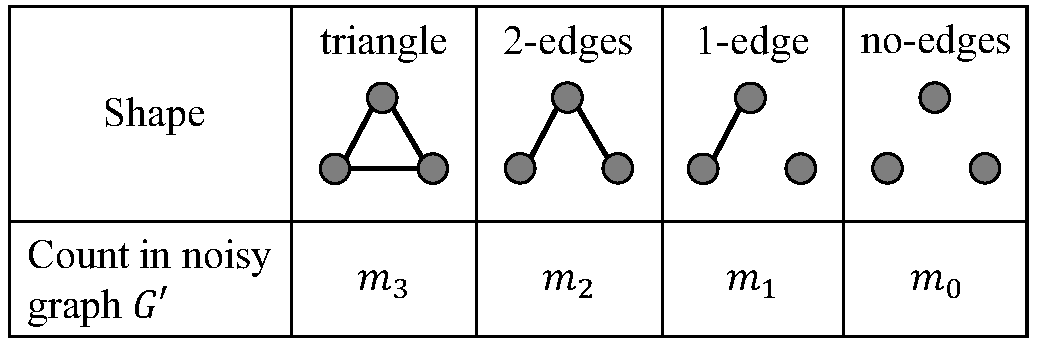
\includegraphics[width=0.9\linewidth]{fig/triplet_shape.pdf}
\vspace{-4mm}
\caption{Four types of subgraphs with three nodes.}
\label{chap1-fig:triplet_shape}
\end{figure}

Through 
% some 
% a 
clever post-processing 
% method 
known as 
% an 
empirical estimation 
% method~
\cite{Kairouz_ICML16,Murakami_USENIX19,Wang_USENIX17},
we are able to obtain an unbiased estimate of $f_\triangle(G)$ 
% with access to just $P$. 
from $G'$. 
Specifically, a subgraph with three nodes can be divided into four types depending on the number of edges. 
Three nodes with three edges form a triangle. 
We refer to three nodes with two edges, one edge, and no edges as \textit{2-edges},  \textit{1-edge}, and  \textit{no-edges}, respectively. 
Figure~\ref{chap1-fig:triplet_shape} shows their shapes. 
% Let $m_3, m_2, m_1, m_0 \in \nnints$ be respectively the number of triangles, 2-edges, 1-edge, and no-edges in $G'$. 
% Note that $\sum_{i=0}^3 m_i = \binom{n}{3}$. 
% The expectation of 
$f_\triangle(G)$ can be expressed using $m_3$, $m_2$, $m_1$, and $m_0$ as follows:

\begin{proposition}\label{chap1-prop:triangle_emp}
  %Let $\mu = e^\epsilon$. 
  Let $G'=(V,E')$ be a noisy graph generated by applying the RR to the lower triangular part of $\bmA$.
  Let $m_3, m_2, m_1, m_0 \in \nnints$ be respectively the number of triangles, 2-edges, 1-edge, and no-edges in $G'$. 
  Then 
  \begin{align}
      %\textstyle{\mathbb{E}\left[ \frac{\mu^3}{(\mu-1)^3} m_3 - \frac{\mu^2}{(\mu-1)^3} m_2 + \frac{\mu}{(\mu-1)^3} m_1 - \frac{1}{(\mu-1)^3} m_0 \right] = f_\triangle(G).}
      \textstyle{\mathbb{E}\left[ \frac{e^{3\epsilon}}{(e^\epsilon-1)^3} m_3 \hspace{-0.5mm}-\hspace{-0.5mm} \frac{e^{2\epsilon}}{(e^\epsilon-1)^3} m_2 \hspace{-0.5mm}+\hspace{-0.5mm} \frac{e^\epsilon}{(e^\epsilon-1)^3} m_1 \hspace{-0.5mm}-\hspace{-0.5mm} \frac{1}{(e^\epsilon-1)^3} m_0 \right] \hspace{-0.5mm} = \hspace{-0.5mm} f_\triangle(G).}
      \label{chap1-eq:triangle_emp}
  \end{align}
\end{proposition}

% This significantly reduces the $l_2$ error. 
Therefore, the data collector can count $m_3$, $m_2$, $m_1$, and $m_0$ from $G'$, and calculate an unbiased estimate of $f_\triangle(G)$ by (\ref{chap1-eq:triangle_emp}). 
% Algorithm~\ref{chap1-alg:subgraph-rr} contains the precise way to do this.
In Appendix~\ref{chap1-sec:RR_emp}, we show that the $l_2$ loss is significantly reduced by this empirical estimation.

\setlength{\algomargin}{4mm}
\begin{algorithm}
  \SetAlgoLined
  \KwData{Graph $G$ 
  %described by distributed 
  represented as 
  neighbor lists $\bma_1,
    \ldots, \bma_n
  \in \{0,1\}^n$, privacy budget $\epsilon \in \nnreals$.}
  \KwResult{Private estimate of $f_\triangle(G)$.}
  \For{$i=1$ \KwTo $n$}{
    %$R_i \leftarrow (RR_{\epsilon}(a_i^1), \ldots, RR_{\epsilon}(a_i^{i-1}))$\;
    $R_i \leftarrow (RR_{\epsilon}(a_{i,1}), \ldots, RR_{\epsilon}(a_{i,i-1}))$\;
    $release(R_i)$\;
  }
  %$G' \leftarrow \texttt{UndirectedGraph}(R_1, \ldots, R_{i-1})$\;
  $G'=(V,E') \leftarrow \texttt{UndirectedGraph}(R_1, \ldots, R_n)$\;
  %\tcc{Counts $T_3,T_2,T_1,T_0$ in $P$.}
  \tcc{Counts $m_3,m_2,m_1,m_0$ in $G'$.}
  %$\hat{\textbf{m}} \leftarrow \texttt{CountSubgraphs}(G',3)$\;
  $(m_3, m_2, m_1, m_0) \leftarrow \texttt{Count}(G')$\;
  %$\mu \leftarrow e^\epsilon$\;
  %\KwRet{$\frac{1}{(\mu-1)^3}(\mu^3 m_3 -\mu^2 m_2 + \mu m_1 - m_0)$}
  \KwRet{$\frac{1}{(e^\epsilon-1)^3}(e^{3\epsilon} m_3 - e^{2\epsilon} m_2 + e^\epsilon m_1 - m_0)$}

  %\caption{CountSubgraphsRR\label{chap1-alg:subgraph-rr}}
  \caption{\alg{LocalRR$_\triangle$}\label{chap1-alg:subgraph-rr}}
\end{algorithm}

Algorithm~\ref{chap1-alg:subgraph-rr} shows this algorithm. 
In line 2, user $v_i$ applies the RR with privacy budget $\epsilon$ (denoted by $RR_\epsilon$) to $a_{i,1}, \ldots, a_{i,i-1}$ 
% (which corresponds to users $v_1, \ldots, v_{i-1}$ with smaller user IDs) 
in her neighbor list $\bma_i$, and outputs $R_i = (RR_\epsilon(a_{i,1}), \ldots, RR_\epsilon(a_{i,i-1}))$. 
In other words, we apply the RR to the lower triangular part of $\bmA$ and there is no overlap between edges sent by users. 
In line 5, the data collector uses a function (denoted by \texttt{UndirectedGraph}) 
that converts the bits of $(R_1, \ldots, R_n)$ into an undirected graph $G'
= (V, E')$ by adding edge $(v_i,v_j)$ with $i>j$ to $E'$ if and only if the $j$-th bit of
$R_i$ is $1$. 
Note that $G'$ is biased, as explained above. 
In line 6, the data collector uses a function (denoted by 
\texttt{Count}) that calculates $m_3$, $m_2$, $m_1$, and $m_0$ from $G'$. 
Finally, the data collector outputs the expression inside the expectation on
the left-hand side of (\ref{chap1-eq:triangle_emp}), which is an unbiased estimator for 
$f_\triangle(G)$ by Proposition~\ref{chap1-prop:triangle_emp}.
We denote this algorithm by \alg{LocalRR$_\triangle$}.

% One subtlety of Algorithm~\ref{chap1-alg:subgraph-rr} is that, since each edge is known by two users, releasing users' edges through the RR may result in disagreements over the noisy edges. User $i$ may claim that he is
% connected to $j$, and user $j$ may claim he is not connected to $i$. 
% To avoid this problem, we assume an ordering on users, and we let user $i$ ignore edge
% $(i,j)$ if $i<j$. This means each edge is the responsibility of just one user.
% Because edge $(i,j)$ is released by user $\max\{i,j\}$, it is technically a
% directed edge. Thus, we let $P$ be the undirected graph formed by taking the
% direction out of all noisy edges released (Line 5).


\smallskip
\noindent{\textbf{Theoretical properties.}}~~\alg{LocalRR$_\triangle$} 
% Algorithm~\ref{chap1-alg:subgraph-rr} 
provides the following guarantee.

\begin{theorem}\label{chap1-thm:subgraph-rr_LDP}
  \alg{LocalRR$_\triangle$} provides $\epsilon$-edge LDP and $\epsilon$-relationship DP.
\end{theorem}

\alg{LocalRR$_\triangle$} does not have the doubling issue (i.e., it provides not $2\epsilon$ but $\epsilon$-relationship DP), because we apply the RR to the lower triangular part of $\bmA$, as explained in Section~\ref{chap1-sub:LDP}.

Unlike the RR and empirical estimation for tabular data \cite{Kairouz_ICML16}, the expected $l_2$ loss of \alg{LocalRR$_\triangle$} is complicated. 
% due to the fact that multiple triangles can involve the same edge. 
To simplify the utility analysis, we assume that $G$ is generated from the Erd\"os-R\'enyi graph distribution $\bmG(n,\alpha)$ with edge existence probability $\alpha$; i.e., each edge in $G$ with $n$ nodes is independently generated with probability $\alpha \in [0,1]$.
% which generates $G=(V,E)$ with $|V|=n$ with

\begin{theorem}\label{chap1-thm:subgraph-rr}
  Let $\bmG(n,\alpha)$ be the Erd\"os-R\'enyi graph distribution with edge existence probability $\alpha \in [0,1]$. 
  Let $p = \frac{1}{e^\epsilon+1}$ and 
  $\beta = \alpha(1-p) + (1-\alpha)p$. 
  Let 
  %$A(G, \epsilon)$ 
  $\hf_{\triangle}(G, \epsilon)$ 
  be the output of 
  %Algorithm~\ref{chap1-alg:subgraph-rr}.
  \alg{LocalRR$_\triangle$}.
  %Suppose 
  %$G \sim \bmG(n,\frac{d_{max}}{n})$, 
  If 
  $G \sim \bmG(n,\alpha)$, 
  %the Erd\"os-R\'enyi graph
  %distribution with parameter $\frac{d_{max}}{n}$.  Then, 
  then for all 
  $\epsilon \in \nnreals$, 
  %$l_2^2(A(G,\epsilon),
  $\mathbb{E}[l_2^2(\hf_{\triangle}(G, \epsilon),
  f_\triangle(G))] = 
  %O(\frac{e^{6\epsilon}}{(e^\epsilon-1)^6}d_{max}n^3)$.
  O\left(\frac{e^{6\epsilon}}{(e^\epsilon-1)^6}\beta n^4\right)$.
  %Furthermore, Algorithm~\ref{chap1-alg:subgraph-rr} provides $\epsilon$-edge LDP.
\end{theorem}

% Note that Theorem~\ref{chap1-thm:subgraph-rr} is a statement about the expected 
% % average $l_2^2$ error
% $l_2$ loss 
% over graphs 
% % $G \sim \bmG(n,\frac{d_{max}}{n})$. 
% $G \sim \bmG(n,\alpha)$. 
% This is less ideal than the case of
% Theorem~\ref{chap1-thm:k-stars} which upper bounds the 
% % $l_2^2$ error 
% $l_2$ loss for all $G \in \calG$. 
% However, 
% % $\textbf{G}(n,\frac{d_{max}}{n})$ 
% $\textbf{G}(n,\alpha)$ 
% is considered a realistic model from which
% graphs of max degree $d_{max}$ are drawn, so Theorem~\ref{chap1-thm:subgraph-rr} is
% still 
% % a strong bound.
% valid. 

Note that we assume the Erd\"os-R\'enyi model only for the utility analysis of \alg{LocalRR$_\triangle$}, and do not assume this model for the other algorithms. 
The upper-bound of \alg{LocalRR$_\triangle$} in Theorem~\ref{chap1-thm:subgraph-rr} is less ideal than the upper-bounds of the other algorithms in that it does not consider all possible graphs $G \in \calG$. 
Nevertheless, we also show that the $l_2$ loss of \alg{LocalRR$_\triangle$} is roughly consistent with Theorem~\ref{chap1-thm:subgraph-rr} in our experiments using two real datasets (Section~\ref{chap1-sec:experiments}) and 
% artificial graphs based on 
the Barab\'{a}si-Albert graphs \cite{NetworkScience}, which have power-law degree distribution (Appendix~\ref{chap1-sec:BAGraph}). 

% The parameter $\alpha$ is very small in a sparse graph. 
% For example, it is reasonable to assume that $\alpha \leq \frac{d_{max}}{n} \ll 1$. 
% On the other hand, $\beta$ is a parameter in 
The parameters $\alpha$ and $\beta$ are edge existence probabilities in the original graph $G$ and noisy graph $G'$, respectively. 
Although $\alpha$ is very small in a sparse graph, $\beta$ can be large for small $\epsilon$. 
For example, if $\alpha \approx 0$ and $\epsilon=1$, then $\beta \approx \frac{1}{e+1} = 0.27$. 
% In this case, the expected $l_2$ loss of \alg{LocalRR$_\triangle$} can be expressed as: $O\left(\frac{e^{6\epsilon}}{(e^\epsilon-1)^6}d_{max} n^3\right)$.

Theorem~\ref{chap1-thm:subgraph-rr} states that for large $n$, the $l_2$ loss of \alg{LocalRR$_\triangle$} 
($=O(n^4)$) 
% ($=O(d_{max}n^3)$) 
is much larger than the $l_2$ loss of \alg{LocalRR$_k\star$} ($=O(n)$). 
This follows from the fact that user $v_i$ 
% cannot see any edge $(v_j, v_k) \in E$ in graph $G$ and 
is not aware of any triangle formed by $(v_i, v_j, v_k)$, as explained above. 

In contrast, counting $f_\triangle(G)$ in the centralized model is much easier because the data collector sees all triangles in $G$; i.e., the data collector knows $f_\triangle(G)$. 
% After we perform graph projection 
% \cite{Day_SIGMOD16,Kasiviswanathan_TCC13,Raskhodnikova_arXiv15} 
% so that each user's degree does not exceed $\td_{max}$, 
% the 
The 
% local 
% global 
sensitivity of $f_\triangle$ 
% becomes 
is 
at most $\td_{max}$ (after graph projection). 
% Therefore, as with $k$-stars, 
Thus, 
we can consider a simple algorithm that 
% performs graph projection so that each user's degree never exceeds $\td_{max}$, 
% and then 
% adds the Laplacian noise $\Lap(\td_{max}/\epsilon)$ 
% ($\td_{max} > d_{max}$) 
% to $f_{\triangle}(G)$, and 
outputs $f_{\triangle}(G) + \Lap(\td_{max}/\epsilon)$. 
We denote this algorithm by \alg{CentralLap$_{\triangle}$}. 
\alg{CentralLap$_{\triangle}$} attains the expected $l_2$ loss ($=$ variance) of $O\left(\frac{\td_{max}^2}{\epsilon^2}\right)$. 

% \colorB{In Section~\ref{chap1-sub:two_rounds}, we propose a two-rounds LDP algorithm for triangles to significantly reduce the $l_2$ loss in the local model.}

% In Algorithm~\ref{chap1-alg:subgraph-rr}, 
The large $l_2$ loss of \alg{LocalRR$_\triangle$} is caused by the fact that 
each edge is released independently with
some probability of being flipped. 
% Thus, 
In other words, 
there are three independent random
variables that influence 
% any subgraph of size $3$ in $P$. 
any triangle in $G'$. 
The next algorithm,
using interaction, 
% is able to reduce 
reduces 
this influencing number 
% to two, 
from three to one 
% because 
% a single 
by using the fact that 
a user 
% always 
knows 
% two edges of a subgraph of size 3.
the existence of two edges for any triangle that involves the user. 

% \ji{Can we combine the last and third-last paragraphs of this section?}
% \tm{It's a little bit difficult to me because 
% the explanation is in the order of ``Thm 4 --> one-round local (third-last) --> centralized (second-last) --> two-round local (last) (--> Sec 4.3)''. Instead, I shortened the third-last paragraph.}

% \subsection{Two-Rounds LDP Algorithms for Triangles}
\subsection{Two-Rounds Algorithms for Triangles}
% \colorB{Sequentially Interactive Graph LDP Algorithms}}
\label{chap1-sub:two_rounds}

\noindent{\textbf{Algorithm.}}~~Allowing for 
% sequential interaction, 
two-rounds interaction, 
we are able to compute $f_{\triangle}$ with
a significantly improved $l_2$ loss, albeit with a higher per-user
communication overhead.
As described in Section~\ref{chap1-sub:non-interactive_triangles}, it is impossible for user $v_i$ to see edge $(v_j, v_k) \in E$ in graph $G=(V,E)$ at the first round. 
However, if 
% each user $v_i$ applies the RR to her neighbor list $\bma_i$ as in \alg{LocalRR$_\triangle$} and 
the data collector publishes a noisy graph $G'=(V,E')$ calculated by \alg{LocalRR$_\triangle$} at the first round, then 
user $v_i$ can see a noisy edge $(v_j, v_k) \in E'$ in the noisy graph $G'$ at the second round. 
Then user $v_i$ can count the number of \textit{noisy triangles} formed by
$(v_i, v_j, v_k)$ such that $(v_i,v_j) \in E$, $(v_i,v_k) \in E$, and $(v_j,v_k)
\in E'$, and send the noisy triangle counts with the Laplacian noise to the data
collector in an analogous way to \alg{LocalLap$_{k\star}$}.
Since user $v_i$ always knows that two edges $(v_i,v_j)$ and $(v_i,v_k)$ exist in $G$, 
there is only one noisy edge in any noisy triangle 
(whereas all edges are noisy in \alg{LocalRR$_\triangle$}).
% edge $(v_j,v_k)$
% random variable 
% that influences the existence of the triangle $(v_i, v_j, v_k)$ in $G$. 
This is an intuition behind our proposed two-rounds algorithm. 

As with the RR in Section~\ref{chap1-sub:non-interactive_triangles}, simply counting the noisy triangles can introduce a bias. 
Therefore, we calculate an empirical estimate of $f_\triangle(G)$ from the noisy triangle counts. 
Specifically, 
% we calculate the expectation of 
the following is the empirical estimate of $f_\triangle(G)$: 
% can be expressed as follows:
% Specifically, assume that the data collector publishes a noisy graph $G'=(V,E')$ calculated by \alg{LocalRR$_\triangle$} with privacy budget $\epsilon_0 \in \nnreals$ at the first round. 
% Let $t_i \in \nnints$ be the number of triplets $(v_i, v_j, v_k)$ such that $j < i < k$, $(v_i,v_j) \in E$, $(v_i,v_k) \in E$, and $(v_j,v_k) \in E'$; i.e., 
% the number of noisy triangles user $v_i$ can see at the second round. 
% Here we count only triplets $(v_i, v_j, v_k)$ with $j < i < k$ to avoid counting the same triplet multiple times.
% Let $s_i \in \nnints$ be the number of triplets $(v_i, v_j, v_k)$ such that $j < i < k$, $(v_i,v_j) \in E$, and $(v_i,v_k) \in E$; i.e., 
% the number of $2$-stars of which user $v_i$ is a center. 
% Then the expectation of $f_\triangle(G)$ can be calculated from $\epsilon_0$, $t_i$, and $s_i$ as follows:

\begin{proposition}\label{chap1-prop:triangle_emp_2rounds}
  Let $G'=(V,E')$ be a noisy graph generated by applying the RR with privacy budget $\epsilon_1 \in \nnreals$   to the lower triangular part of $\bmA$.
  Let $p_1 = \frac{1}{e^{\epsilon_1}+1}$. 
  Let $t_i \in \nnints$ be the number of triplets $(v_i, v_j, v_k)$ such that 
  %$j < i < k$, 
  $j < k < i$, 
  $(v_i,v_j) \in E$, $(v_i,v_k) \in E$, and $(v_j,v_k) \in E'$.
  Let $s_i \in \nnints$ be the number of triplets $(v_i, v_j, v_k)$ such that 
  %$j < i < k$, 
  $j < k < i$, 
  $(v_i,v_j) \in E$, and $(v_i,v_k) \in E$. 
  Let $w_i = t_i - p_1 s _i$. 
  Then 
  \begin{align}
      %\textstyle{\mathbb{E}[f_\triangle(G)] = \frac{1}{1-2p_1} \sum_{i=1}^n (t_i - p_1 s_i)}.
      \textstyle{\mathbb{E}\left[ \frac{1}{1-2p_1} \sum_{i=1}^n w_i \right] = f_\triangle(G).}
      \label{chap1-eq:triangle_emp_2rounds}
  \end{align}
\end{proposition}

Note that in Proposition~\ref{chap1-prop:triangle_emp_2rounds}, 
we count only triplets $(v_i, v_j, v_k)$ with 
% $j < i < k$ 
$j < k < i$ 
% to avoid counting the same triplet multiple times. 
to use only the lower triangular part of $\bmA$. 
$t_i$ is the number of noisy triangles user $v_i$ can see at the second round. 
$s_i$ is the number of $2$-stars of which user $v_i$ is a center. 
Since $t_i$ and $s_i$ can reveal information about an edge in $G$, user $v_i$ adds the Laplacian noise to $w_i$ $(= t_i - p_1 s _i)$ in (\ref{chap1-eq:triangle_emp_2rounds}), and sends it to the data collector. 
Then the data collector calculates an unbiased estimate of $f_\triangle(G)$ by (\ref{chap1-eq:triangle_emp_2rounds}). 

% Instead of releasing each edge through 
% randomized
% response, user $i$ is given a specific query depending on $P_{i-1}$, the
% subgraph of $G$ on users $1$ through $i-1$ released through randomized response.
% Like Algorithm~\ref{chap1-alg:subgraph-rr}, we assume user $i$ ignores edge $(i,j)$ if
% $i<j$. The query to user $i$ is to noisily count the number of triangles of which he is
% a part, using two of his edges and one edge in $P_{i-1}$. He releases this
% number and a randomized response on his edges so that future users may build
% $P_{i}$. 

\setlength{\algomargin}{5mm}
\begin{algorithm}
  \SetAlgoLined
  \KwData{Graph $G$ 
  %described by distributed 
  represented as 
  neighbor lists $\bma_1,
    \ldots, \bma_n
    \in \{0,1\}^n$, two privacy budgets
  %$\epsilon_0,\epsilon_1 > 0$.}
  $\epsilon_1,\epsilon_2 > 0$, $\td_{max} \in \nnints$.}
  %\KwResult{Private count of number of triangles in $G$.}
  \KwResult{Private estimate of $f_\triangle(G)$.}
  %$\rho \leftarrow \frac{1}{e^{\epsilon_0}+1}$\;
  $p_1 \leftarrow \frac{1}{e^{\epsilon_1}+1}$\;
  \tcc{First round.}
  \For{$i=1$ \KwTo $n$}{
    %$ans_i \leftarrow 0$\;
    %$R_i \leftarrow (RR_{\epsilon_0}(a_i^1), \ldots, RR_{\epsilon_0}(a_i^{i-1}))$\;
    $R_i \leftarrow (RR_{\epsilon_1}(a_{i,1}), \ldots, RR_{\epsilon_1}(a_{i,i-1}))$\;
    $release(R_i)$\;
  }
  %$P_{i-1} \leftarrow \texttt{UndirectedGraph}(R_1, \ldots, R_{i-1})$\;
  $G'=(V,E') \leftarrow \texttt{UndirectedGraph}(R_1, \ldots, R_{i-1})$\;
  \tcc{Second round.}
  \For{$i=1$ \KwTo $n$}{
    $\bma_i \leftarrow \texttt{GraphProjection}(\bma_i, \td_{max})$\;
    %$t_i \leftarrow |\{(u,v) : u,v \in [i], u<v<i, a_{i}^u = a_{i}^v = 1,(u,v) \in P_{i-1}\}|$\;
    $t_i \leftarrow |\{(v_i,v_j,v_k) : 
    %j<i<k, a_{j,i} = a_{i,k} = 1, 
    j<k<i, a_{i,j} = a_{i,k} = 1, 
    (v_j,v_k) \in E'\}|$\;
    %$s_i \leftarrow |\{(u,v) : u,v \in [i], u<v<i, a_{i}^u = a_{i}^v = 1\}|$\;
    $s_i \leftarrow |\{(v_i,v_j,v_k) : 
    %j<i<k, a_{j,i} = a_{i,k} = 1\}|$\;
    j<k<i, a_{i,j} = a_{i,k} = 1\}|$\;
    %$w_i \leftarrow t_i - \rho s_i + Lap(\frac{d_{max}(1-\rho)}{\epsilon_1})$\;
    %$w_i \leftarrow t_i - p_1 s_i + \Lap(\frac{\td_{max}(1-p_1)}{\epsilon_2})$\;
    $w_i \leftarrow t_i - p_1 s_i$\;
    $\hw_i \leftarrow w_i + \Lap(\frac{\td_{max}}{\epsilon_2})$\;
    %$release(R_i, w_i)$\;
    $release(\hw_i)$\;
  }
  %$ans \leftarrow \frac{1}{1-2\rho}\sum_{i=1}^n w_i$\;
  \KwRet{$\frac{1}{1-2p_1}\sum_{i=1}^n \hw_i$}
  %\caption{CountSubgraphsTwoRound\label{chap1-alg:subgraph-interactive}}
  \caption{\alg{Local2Rounds$_\triangle$}}\label{chap1-alg:subgraph-interactive}
\end{algorithm}

Algorithm~\ref{chap1-alg:subgraph-interactive} contains the formal
description of this process. 
It takes as input a graph $G$, 
% (represented as neighbor lists $\bma_1, \ldots, \bma_n$), 
the privacy budgets $\epsilon_1, \epsilon_2 \in \nnreals$ at the first and second rounds, respectively, 
and 
% It also takes as input 
% an upper-bound $\td_{max}$ on the maximum degree $d_{max}$ of $G$ 
a non-negative integer $\td_{max} \in \nnints$. 
% in the same way as \alg{LocalLap$_{k\star}$}. 
% We will describe the private computation of $d_{max}$ with edge LDP at the end of Section~\ref{chap1-sub:two_rounds}. 
At the first round, we 
apply the RR to the lower triangular part of $\bmA$ 
(i.e., there is no overlap between edges sent by users) 
% . 
and use the \texttt{UndirectedGraph} function to 
obtain a noisy graph $G'=(V,E')$ by the RR in the same way as Algorithm~\ref{chap1-alg:subgraph-rr}. 
Note that $G'$ is biased. 
We calculate an unbiased estimate of $f_\triangle(G)$ from $G'$ at the second round.  
% Then we use the \texttt{UndirectedGraph} function, which makes an undirected graph $G'
% = (V, E')$ by adding edge $(i,j)$ with $i>j$ to $E'$ if and only if the $j$-th bit of $R_i$ is $1$. 

At the second round, each user $v_i$ 
calculates $\hw_i = w_i + \Lap(\frac{\td_{max}}{\epsilon_2})$ 
%  and 
by adding the Laplacian noise to $w_i$ 
% $(= t_i - p_1 s _i)$, 
in Proposition~\ref{chap1-prop:triangle_emp_2rounds} 
whose 
% local 
% global 
sensitivity is at most 
% $d_{max} (1-p_1)$, 
$\td_{max}$ 
% (after graph projection), 
(as we will prove in Theorem~\ref{chap1-thm:local2rounds_LDP}). 
Finally, we output $\frac{1}{1-2p_1}\sum_{i=1}^n \hw_i$, which is an unbiased estimate of $f_\triangle(G)$ by Proposition~\ref{chap1-prop:triangle_emp_2rounds}. 
We call this algorithm \alg{Local2Rounds$_\triangle$}.

% The intuitive reason Algorihtm~\ref{chap1-alg:subgraph-interactive} performs better than 
% Algorithm~\ref{chap1-alg:subgraph-rr} is that a noisy triangle is counted using two 
% noisy computations, the noisy edge in
% $P_{i-1}$ and user $i$'s noisy count. In Algorithm~\ref{chap1-alg:subgraph-rr}, each
% subgraph of size $3$ in $P$ is the result of three noisy computations.

\smallskip
\noindent{\textbf{Theoretical properties.}}~~\alg{Local2Rounds$_\triangle$} 
% Algorithm~\ref{chap1-alg:subgraph-interactive} 
has the following 
% performance 
guarantee.

\begin{theorem}\label{chap1-thm:local2rounds_LDP}
  %If the maximum degree $d_{max}$ of $G$ is at most $\td_{max}$, 
  \alg{Local2Rounds$_\triangle$}
  provides $(\epsilon_1 + \epsilon_2)$-edge LDP and $(\epsilon_1 + \epsilon_2)$-relationship DP.
\end{theorem}

As with \alg{LocalRR$_\triangle$}, \alg{Local2Rounds$_\triangle$} does not have the doubling issue; i.e., it provides $\epsilon$-relationship DP (not $2\epsilon$). 
This follows from the fact that we 
use only the lower triangular part of $\bmA$; 
% count each triplet $(v_i,v_j,v_k)$ only once; 
i.e., we assume 
%$j<i<k$ 
$j<k<i$ 
in counting $t_i$ and $s_i$. 

\begin{theorem}\label{chap1-thm:local2rounds}
  Let 
  %$A(G, d_{max}, \epsilon_0, \epsilon_1)$ 
  $\hf_{\triangle}(G, \epsilon_1, \epsilon_2, \td_{max})$ 
  be the output of 
  %Algorithm~\ref{chap1-alg:subgraph-interactive}. 
%   \alg{LocalRR$_\triangle$}. 
  \alg{Local2Rounds$_\triangle$}. 
  Then, for all 
  %$d_{max} \in \nats$,
  $\epsilon_1,\epsilon_2 \in \nnreals$, 
  $\td_{max} \in \nnints$,
  and $G\in \calG$ such that the
  maximum degree $d_{max}$ of $G$ is 
  at most 
  $\td_{max}$,
  %$l_2^2(A(G,d_{max},\epsilon_0,\epsilon_1) 
  $\mathbb{E}[l_2^2(\hf_{\triangle}(G, \epsilon_1, \epsilon_2, \td_{max}), f_\triangle(G))] 
  \leq
    O\left(\frac{e^{\epsilon_1}}{(1-e^{\epsilon_1})^2} \left(\td_{max}^3 n +
    \frac{e^{\epsilon_1}}{\epsilon_2^2}\td_{max}^2 n\right)\right)$.
\end{theorem}

Theorem~\ref{chap1-thm:local2rounds} means that for triangles, the $l_2$ loss 
% of \alg{LocalRR_$\triangle$} 
is reduced from $O(n^4)$ to $O(\td_{max}^3n)$ by introducing an additional round. 

% The upper and lower bounds on the $l_2$ losses for the central,
% % local non-interactive, 
% one-round local, 
% and 
% % local sequentially interactive 
% two-rounds local 
% models discussed in
% this section appear in Table~\ref{chap1-tab:perf}.

\smallskip
\noindent{\textbf{Private calculation of $d_{max}$.}}~~As with $k$-stars, we can privately calculate $d_{max}$ 
% with edge LDP 
by using the method described in Section~\ref{chap1-sub:non-interactive_k_stars}. 
Furthermore, the private calculation of $d_{max}$ does not increase the number of rounds; i.e., we can run \alg{Local2Rounds$_\triangle$} with the private calculation of $d_{max}$ in two rounds. 

Specifically, let $\epsilon_0 \in \nnreals$ be the privacy budget for the private calculation of $d_{max}$. 
At the first round, each user $v_i$ adds $\Lap(\frac{1}{\epsilon_0})$ to her degree $d_i$, 
% (i.e., number of ``$1$''s in her neighbor list $\bma_i$), 
and sends the noisy degree $\hd_i$ ($=d_i + \Lap(\frac{1}{\epsilon_0})$) to the data collector, along with the outputs $R_i = (RR_\epsilon(a_{i,1}), \ldots, RR_\epsilon(a_{i,i-1}))$ of the RR. 
The data collector calculates the noisy max degree $\hd_{max}$ ($= \max\{\hd_1,
\ldots, \hd_n\}$) as an estimate of $d_{max}$, and sends it back to all users. 
At the second round, we run \alg{Local2Rounds$_\triangle$} with input $G$ (represented as $\bma_1, \ldots, \bma_n$), $\epsilon_1$, $\epsilon_2$, and $\lfloor \hd_{max} \rfloor$. 

% At the second round, each user performs graph projection; i.e., if $d_i$ exceeds $\hd_{max}$, user $v_i$ randomly selects $\hd_{max}$ neighbors from her neighbor list $\bma_i$ (otherwise, user $v_i$ uses $\bma_i$ as it is). 
% Let $\bma'_i \in \{0,1\}^n$ be a neighbor list of user $v_i$ after this projection. 
% We run the second round part (lines $7$ to $12$) of \alg{Local2Rounds$_\triangle$} with input $\bma'_1, \ldots, \bma'_n$, $\epsilon_1$, $\epsilon_2$, 
% and $\hd_{max}$. 

At the first round, the calculation of $\hd_{max}$ provides $\epsilon_0$-edge LDP. 
% because each user's degree has the sensitivity $1$ under edge LDP. 
Note that it provides $2\epsilon_0$-relationship DP (i.e., it has the doubling issue) because one edge $(v_i,v_j) \in E$ affects both of the degrees $d_i$ and $d_j$ by 1. 
At the second round, \alg{LocalLap$_{k\star}$} provides $(\epsilon_1 + \epsilon_2)$-edge LDP and 
$(\epsilon_1 + \epsilon_2)$-relationship DP (Theorem~\ref{chap1-thm:local2rounds_LDP}). 
% because each user $v_i$'s degree in $\bma'_i$ never exceeds $\hd_{max}$. 
% (and then Theorem~\ref{chap1-thm:local2rounds_LDP} holds). 
Then by the composition theorem~\cite{DP}, this two-rounds algorithm provides $(\epsilon_0 + \epsilon_1 + \epsilon_2)$-edge LDP and $(2\epsilon_0 + \epsilon_1 + \epsilon_2)$-relationship DP. 
Although the total privacy budget is larger for relationship DP, the difference ($=\epsilon_0$) can be very small. 
In fact, we set $(\epsilon_0, \epsilon_1, \epsilon_2) = (0.1, 0.45, 0.45)$ or $(0.2, 0.9, 0.9)$ in our experiments (i.e., the difference is $0.1$ or $0.2$), and show that this algorithm provides almost the same utility as \alg{Local2Rounds$_\triangle$} with the true max degree $d_{max}$. 

\smallskip
\noindent{\textbf{Time complexity.}}~~We also note that \alg{Local2Rounds$_\triangle$} has an advantage over \alg{LocalRR$_\triangle$} in terms of the time complexity. 
% in addition to the expected $l_2$ loss. 

Specifically, \alg{LocalRR$_\triangle$} is inefficient because the data collector has to count the number of triangles $m_3$ in the noisy graph $G'$. 
Since the noisy graph $G'$ is dense (especially when $\epsilon$ is small) and there are $\binom{n}{3}$ subgraphs with three nodes in $G'$, the number of triangles is $m_3 = O(n^3)$. 
Then, the time complexity of \alg{LocalRR$_\triangle$} is 
% $O(n)$ for each user's part and $O(n^3)$ for the data collector's part, 
also $O(n^3)$, which is not practical for a graph with a large number of users $n$.
In fact, we implemented \alg{LocalRR$_\triangle$} ($\epsilon=1$) with C/C++ and measured its running time using one node of a supercomputer (ABCI: AI Bridging Cloud Infrastructure \cite{ABCI}). 
When $n=5000$, $10000$, $20000$, and $40000$, the running time was $138$, $1107$, $9345$, and $99561$ seconds, respectively; i.e., the running time was almost cubic in $n$. 
We can also estimate the running time for larger $n$. 
For example, when $n=1000000$, \alg{LocalRR$_\triangle$} ($\epsilon=1$) would require about $35$ years $(=1107 \times 100^3 /(3600 \times 24 \times 365))$. 
% Even if we use $1000$ nodes of the supercomputer (the ABCI has $1088$ nodes \cite{ABCI}) in parallel, \alg{LocalRR$_\triangle$} would require over $10$ days. 

In contrast, the time complexity of \alg{Local2Rounds$_\triangle$} 
% for each user 
is 
% $O(n)$ in the first round (l.3-4 in Algorithm~\ref{chap1-alg:subgraph-interactive}) and $O(d_{max}^2)$ in the second round (l.8-13 in Algorithm~\ref{chap1-alg:subgraph-interactive})). 
% $O(n + d_{max}^2)$ for each user's part and $O(n)$ for the data collector's part at the second round. 
$O(n^2 + n d_{max}^2)$\footnote{When we 
% want to 
evaluate 
% the utility of 
\alg{Local2Rounds$_\triangle$} in our experiments, 
% When we evaluate the utility of \alg{Local2Rounds$_\triangle$} on one computer, 
we can apply the RR to only edges that are required at the second round; i.e., $(v_j,v_k) \in G'$ in line 8 of Algorithm~\ref{chap1-alg:subgraph-interactive}. 
Then the time complexity of \alg{Local2Rounds$_\triangle$} 
% is 
can be reduced to 
$O(n d_{max}^2)$ in total. 
We also confirmed that when $n=1000000$, the running time of \alg{Local2Rounds$_\triangle$} was $311$ seconds on one node of the ABCI. 
% , which is $3.5 \times 10^6$ times faster than \alg{LocalRR$_\triangle$}. 
Note, however, that this does \textit{not} protect individual privacy, because it reveals the fact that users $v_j$ and $v_k$ are friends with $u_i$ to the data collector.}. 
% including the private calculation of $d_{max}$. 
The factor of $n^2$ comes from the fact that the size of the noisy graph $G'$ is $O(n^2)$. 
This also causes a large communication overhead, as explained below.
% Further reduction of the time complexity by compressing the graph size (e.g., via graph projection) is left for future work.}

\smallskip
\noindent{\textbf{Communication overhead.}}~~In 
% The \alg{Local2Rounds$_\triangle$} has a quadratic communication overhead.
\alg{Local2Rounds$_\triangle$}, each user need to see the noisy graph $G'$ 
of size $O(n^2)$ 
% with $O(n^2)$ bits 
to count $t_i$ and $s_i$. 
% must count $t_i$ and $s_i$ which depend on $G'$, the private graph computed in the first round. 
% Thus, each user must see $G'$, a graph with $O(n^2)$ bits. 
This results in a per-user communication overhead of $O(n^2)$. 
% We 
Although we 
do not simulate the communication overhead in our experiments that use \alg{Local2Rounds$_\triangle$}, 
% but 
the $O(n^2)$ overhead 
% would 
might 
limit its application in very large graphs. 
An interesting avenue of future work is how to compress the graph size (e.g., via graph projection or random projection) to reduce both the time complexity and the communication overhead.
% Again, compressing the graph size (e.g., via graph projection) is left for future work.

\begin{table*}
  \centering
\begin{tabular}{|l|l|l|l|l|l|l|}
  \hline
  & Centralized & \spantwo{One-round local} & Two-rounds local \\
  \hline
  & Upper Bound & Lower Bound & Upper Bound & Upper Bound \\ \hline

  $f_{k\star}$
  & $O\left( \frac{d_{max}^{2k-2}}{\epsilon^2} \right)$  
  &  $\Omega\left( \frac{e^{2\epsilon}}{(e^{2\epsilon}+1)^2}d_{max}^{2k-2}n \right)$ 
  &  $O\left( \frac{d_{max}^{2k-2}}{\epsilon^2}n \right)$ 
  &  $O\left( \frac{d_{max}^{2k-2}}{\epsilon^2}n \right)$ \\ \hline

 $f_\triangle$ 
  &  $O\left(\frac{d_{max}^2}{\epsilon^2}\right)$ 
  &  $\Omega\left( \frac{e^{2\epsilon}}{(e^{2\epsilon}+1)^2}d_{max}^2n \right)$
  &  $O\left(\frac{e^{6\epsilon}}{(e^{\epsilon}-1)^6}n^4\right)$ 
  (when $G \sim \bmG(n,\alpha)$)
  %(randomized bound)
  &  $O\left(\frac{e^\epsilon}{(e^\epsilon-1)^2}(d_{max}^3 n +
  \frac{e^\epsilon}{\epsilon^2}d_{max}^2 n)\right)$ \\ \hline

\end{tabular}
% \vspace{-3.5mm}
\vspace{-2mm}
\caption{Bounds on $l_2$ losses for privately estimating $f_{k\star}$ and
$f_{\triangle}$ with $\epsilon$-edge LDP. For upper-bounds, we assume that  $\td_{max}=d_{max}$. 
For the centralized model, we use the Laplace mechanism. For
the one-round $f_\triangle$ algorithm, we apply Theorem~\ref{chap1-thm:subgraph-rr} 
with constant $\alpha$. For the two-round protocol $f_\triangle$ algorithm, we
apply Theorem~\ref{chap1-thm:local2rounds} with
$\epsilon_1=\epsilon_2=\frac{\epsilon}{2}$. }\label{chap1-tab:perf}
\end{table*}

\subsection{Lower Bounds}
\label{chap1-sub:lower_bounds}

We show a general lower bound on the $l_2$ loss of private estimators $\hat{f}$ of
real-valued functions $f$ in the one-round LDP model. Treating $\epsilon$ as a
constant, we have shown that 
when $\td_{max}=d_{max}$, 
% for graphs $G$ of maximum degree $d_{max}$,
the expected $l_2$ loss of \alg{LocalLaplace$_{k\star}$} is 
% $l_2^2(\alg{LocalLaplace$_{k\star}$}(G), f_{k\star}(G)) = 
$O(nd_{max}^{2k-2})$
(Theorem~\ref{chap1-thm:k-stars}). 
% and 
% the expected $l_2$ loss of 
% \alg{Local2Rounds$_\triangle$} is 
% \alg{LocalRR$_\triangle$} is 
%$l_2^2(\alg{LocalRR$_\triangle$}(G),
% f_{k\star}(G) ) = 
% $O(nd_{max}^2)$ 
% $O(nd_{max}^3)$ 
% $O(n^4)$ 
% (Theorem~\ref{chap1-thm:local2rounds}). 
% (Theorem~\ref{chap1-thm:subgraph-rr}). 
However, in
the centralized 
% edge-DP 
model, we can use
the Laplace mechanism with sensitivity 
$2\binom{d_{max}}{k-1}$ 
% and 
%$d_{max}^2$,
% $d_{max}$ 
% respectively, 
to obtain $l_2^2$ errors of $O(d_{max}^{2k-2})$ 
% and
% $O(d_{max}^2)$, respectively 
for $f_{k\star}$. 
% and $f_\triangle$. 
Thus, we ask
if 
% the factors of $n$ are 
the factor of $n$ is 
necessary 
% in the local model. 
in the one-round LDP model.

We 
% partially 
answer this question affirmatively.
We show for many types of queries $f$, there is a lower bound on 
% $l_2^2(f(\bmA), \hf(\bmA))$ 
$l_2^2(f(G), \hf(G))$ 
for any private estimator $\hf$ of the form
\begin{equation}\label{chap1-eq:one-round-lower}
%   \hf(\bmA) = \tilde{f}(\calR_1(\bma_1), \ldots, \calR_n(\bma_n)).
  \hf(G) = \tilde{f}(\calR_1(\bma_1), \ldots, \calR_n(\bma_n)),
\end{equation}
where 
$\calR_1, \ldots, \calR_n$ satisfy 
% $\epsilon$-relationship or $\epsilon$-edge DP 
$\epsilon$-edge LDP or $\epsilon$-relationship DP 
and $\tilde{f}$ is an aggregate function that takes $\calR_1(\bma_1), \ldots, \calR_n(\bma_n)$ as input and outputs $\hf(G)$. 
Here we assume that $\calR_1, \ldots, \calR_n$ 
% and 
are independently run, meaning that they are in the one-round
setting.
% 
% Our lower bound has the form of $\Omega(nD^2)$, where $D$ is a positive real
% number depending on $f$ that is similar to, but stronger than, the global sensitivity $GS_f$.
% Global sensitivity by itself cannot provide a strong lower bound in the
% local model. As a counterexample, if $f$ were the function that is always $0$ or $GS_f$,
% then an estimator $\hf$ that predicts $0$ would satisfy
% $l_2^2(f(\bmA),\hf(\bmA)) = O(GS_f^2)$
% for all adjacency matrices $\bmA$. 
% 
% Instead, we 
For our 
%this 
lower bound,
% we consider $f$ to be a function on graphs. 
% not matrices. 
% Then 
% We 
we 
require 
that 
input edges to $f$ 
% to 
be ``independent'' in the sense that 
% and 
adding an edge to an input graph $G$  
independently 
% increase 
change 
$f$ by at least $D \in \reals$. 
% over a set of input graphs. 
% Notice that we consider $f$ to be a function on graphs, not
% matrices, for this lower bound. 
The specific structure of input graphs we require is as follows:

\begin{definition}\label{chap1-def:mono-cube}[$(n,D)$-independent cube for $f$]
  Let 
  %$D \in \reals$. 
  $D \in \nnreals$. 
  For 
  %$k \in \nats$, 
  $\kappa \in \nats$, 
  let $G=(V,E) \in \calG$ be a graph on 
  %$n = 2k$ 
  $n = 2\kappa$ 
  nodes, and let 
  %$M = \{(v_{i_1}, v_{i_2}),(v_{i_3},v_{i_4}),\ldots,(v_{i_{2k-1}},v_{i_{2k}})\}$ 
  $M = \{(v_{i_1}, v_{i_2}),(v_{i_3},v_{i_4}),\ldots,(v_{i_{2k-1}},v_{i_{2\kappa}})\}$ 
  for integers $i_j \in [n]$ 
  %denote 
  be 
  a set of edges such that each of $i_1, \ldots, i_{2\kappa}$ is distinct (i.e., perfect matching on the nodes).
%   a perfect
%   matching on the 
%   nodes, 
%   meaning each 
%   of $i_1, \ldots, i_{2k}$ 
%   is distinct. 
  %Furthermore,
  Suppose that 
  %the perfect matching 
  $M$ is disjoint from 
  $E$; 
  %$G$; 
  i.e., 
  % , meaning 
  %$(v_{i_{2j-1}}, v_{i_{2j-2}}) \notin G$. 
  %$(v_{i_{2j-1}}, v_{i_{2j}}) \notin G$ 
  $(v_{i_{2j-1}}, v_{i_{2j}}) \notin E$ 
  for any 
  %$j\in[k]$. 
  $j\in[\kappa]$. 
  Let 
%   $\calA = \{G \cup N : N \subseteq M\}$.
  $\calA = \{(V, E \cup N): N \subseteq M\}$.
  %Notice 
  Note that 
  $\calA$ is a set of 
  %$2^k$ 
  $2^\kappa$ 
  graphs.
  We say $\calA$ 
  %defines 
  %forms 
  is 
  an \emph{$(n,D)$-independent cube for $f$} if for all
  %$G_1, G_2 \in \calA$ such that $|G_1| + 1 = |G_2|$, 
  $G'=(V,E') \in \calA$, 
  %$G \in \calA$, 
  we have
  \[
    % f(G) = f(G') + \sum_{e \in M} \textbf{1}[e \in G] C_e
    f(G') = f(G) + \sum_{e \in E' \cap M} C_e,
  \]
  where $C_e \in \reals$ satisfies $|C_e| \geq D$ for any $e \in M$.
%   for non-negative real numbers 
%   $\{C_e : e \in M, |C_e| \geq D\}$.}
%   for real numbers 
%   $\{C_e : e \in M\}$ satisfying $|C_e| \geq D$.
\end{definition}

\begin{figure}[t]
  \centering
%   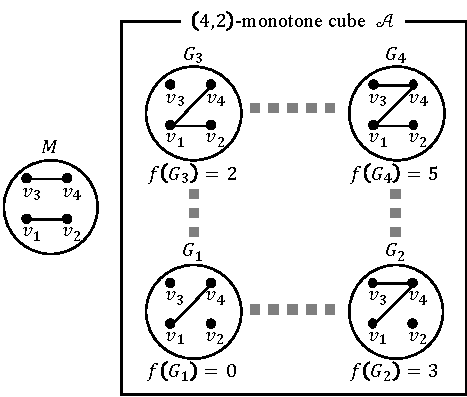
\includegraphics[width=0.88\linewidth]{fig/MonoCube.pdf}
  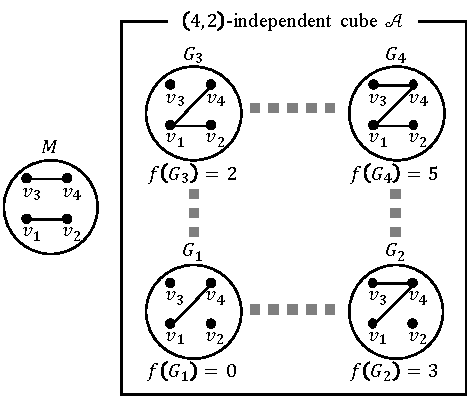
\includegraphics[width=0.9\linewidth]{fig/IndCube.pdf}
  \vspace{-2mm}
  \caption{
    $(4,2)$-independent cube $\calA$ for $f$. 
    In this example, $M = \{(v_1,v_2),(v_3,v_4)\}$, $G_1=(V,E)$, $\calA = \{(V, E \cup N): N \subseteq M\}$, 
    $C_{(v_1,v_2)}=2$, and $C_{(v_3,v_4)}=3$.
    %Definition~\ref{chap1-def:mono-cube} requires that $f$ increase by at least $D=2$ along the dotted gray lines, which it does.
    Adding $(v_1,v_2)$ and $(v_3,v_4)$ increase $f$ by $2$ and $3$, respectively.
  }\label{chap1-fig:mono-cube}
\end{figure}

\begin{figure}[t]
  \centering
  %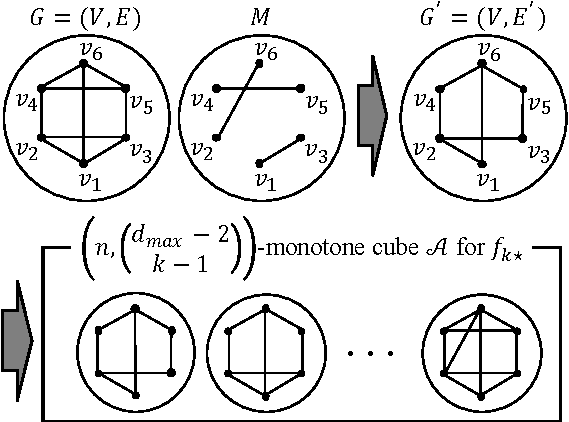
\includegraphics[width=0.88\linewidth]{fig/MonoCube_kstar.pdf}
  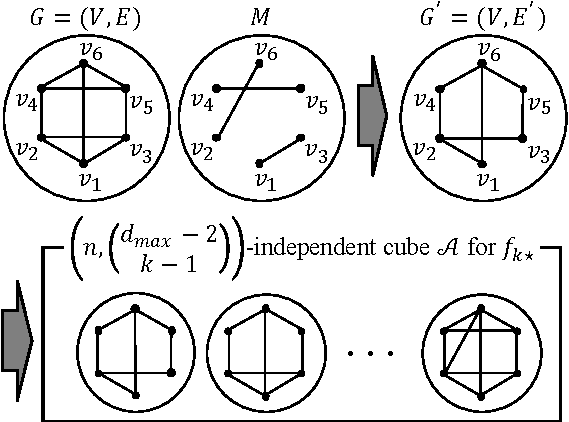
\includegraphics[width=0.9\linewidth]{fig/IndCube_kstar.pdf}
  \vspace{-2mm}
  \caption{
    Construction of an independent cube for a $k$-star function ($n=6$, $d_{max}=4$). 
    From a 
    %$(d_{max} - 1)$-
    $3$-regular graph $G=(V,E)$ and $M=\{(v_1,v_3),(v_2,v_6),(v_4,v_5)\}$, we make a graph $G'=(V,E')$ such that $E' = E \setminus M$. 
    Then $\calA = \{(V, E' \cup N): N \subseteq M\}$ forms an
    $(n, 2\binom{d_{max}-2}{k-1})$-independent cube for $f_{k\star}$.
  }\label{chap1-fig:mono-cube_kstar}
\end{figure}

% We show how to construct an $(n, \binom{d_{max}-3}{k-1})$ monotone cube
% $\mathcal{A}_{k\star}$ for
% $f_{k\star}$. First, we have to take care of a technicality.
% Note that $f_{k\star}(\bmA)$ only operates on symmetric graphs. We extend it to 
% general graphs in a natural way: let $f_{k\star}^{ext}(\bmA)$
% count the number of pointed-out $k$-stars in $\bmA$. Let
% $sym(\mathcal{A})$ be only those matrices in $\mathcal{A}$ that are symmetric,
% corresponding to undirected graphs. We show in the Appendix
% that if $\hf$ privately estimates $f_{k\star}^{ext}$ in the one-round
% edge LDP model, then there is a private estimator $\hat{g}$ that estimates
% $f_{k\star}$ in the one-round edge-LDP model such that
% \begin{multline}\label{chap1-eq:sym-lower-bound}
%   \E_{\bmA \sim U(\mathcal{A}_{k\star})}[l_2^2(f^{ext}_{k\star}(\bmA),
%   \hf(\bmA))] \\ \leq 
%   \E_{\bmA \sim U(sym(\mathcal{A}_{k\star}))} [l_2^2(f_{k\star}(\bmA),
%   \hf(\bmA))] + O(D^2)
% \end{multline}

Such a set of inputs has an ``independence'' property because,
regardless of which edges from $M$ has been added before, adding edge $e \in M$
always changes $f$ by $C_e$. 
Figure~\ref{chap1-fig:mono-cube} shows an example of a $(4,2)$-independent cube for $f$. 

% For example, 
We can also construct 
% an
% Our 
% $(n,\binom{d_{max}-3}{k-1})$ 
% $(n,\binom{d_{max}-4}{k-1})$ 
a independent cube for 
a $k$-star function 
% on directed graphs 
as follows. 
% $f_{k\star}^{ext}$ is the
% following:
% Assume $d_{max}$ and $n$ are both even. 
Assume that $n$ is even. 
It is well known in graph theory that if $n$ is even, then 
for any $d\in[n-1]$, there exists a 
$d$-regular graph where every node has degree $d$ \cite{Ganesan_arXiv18}. 
%Assume $n$ and $d_{max}$ are even and 
Therefore, there exists a 
% Let $G \in \calG$ be a $(d_{max}-1)$-regular graph 
$(d_{max}-1)$-regular graph $G=(V,E)$ 
of size $n$. 
% or a graph 
% in which every node has degree $d_{max}-1$. 
% It is a standard result in graph theory that 
% for any $d\in[n-1]$, 
% $d$-regular graphs exist 
% % for all $d$ 
% when $n$ is even.
Pick an arbitrary perfect matching $M$ on the nodes. Now, let 
% $G' = G \setminus M$. 
$G' = (V,E')$ such that $E' = E \setminus M$. 
Every node in $G'$ has degree between $d_{max}-2$ and $d_{max}-1$. 
Adding an edge in $M$ to $G'$ will produce at least
$2\binom{d_{max}-2}{k-1}$ new $k$-stars.
%the resulting graph be $\bmA = \{\bma_1,\ldots, \bma_n\}$.
%The collection $\prod_{i=1}^n \{\bma_i, \bma_i'\}$ (where the product is the Cartesian product) 
%forms an
% $(n,\binom{d_{max}-3}{k-1})$ 
% $(n,\binom{d_{max}-4}{k-1})$ 
Thus, $\calA = \{(V, E' \cup N): 
% G' \cup N : 
N \subseteq M\}$ forms an
$(n, 2\binom{d_{max}-2}{k-1})$-independent cube for $f_{k\star}$. 
% for $f_\triangle^{ext}$ 
% $\binom{d_{max}-3}{k-1}$ 
% $\binom{d_{max}-4}{k-1}$ 
%Similarly, for even natural number $l \in \nats$ such that $d_{max}>l+2$, we can construct an $(n,\binom{d_{max}-l-2}{k-1})$ monotone cube from the adjacency matrix of a collection of cliques of size $d_{max}-l$.
Note that the maximum degree of each graph in $\calA$ is at most $d_{max}$. 
Figure~\ref{chap1-fig:mono-cube_kstar} shows how to construct an independent cube for a $k$-star function when $n=6$ and $d_{max}=4$. 

% Let $U(\mathcal{A})$ be the uniform distribution over an $(n,D)$ monotone cube $\mathcal{A}$. 
Using the structure that the $(n,D)$-independent cube imposes on $f$,
we can prove a lower bound:
\begin{theorem}\label{chap1-thm:lower-bound}
  Let 
  %$\hf(\bmA)$ 
  $\hf(G)$ 
  have the form of~\eqref{chap1-eq:one-round-lower}, 
  where $\calR_1, \ldots, \calR_n$ are independently run.
  %Assume that 
  %$(\calR_1, \ldots, \calR_n)$ 
  %satisfy 
  %provide 
  %$\epsilon$-relationship DP. 
  %and are independently run.
  Let $\cal{A}$ be an $(n,D)$-independent cube for $f$. 
  If 
  $(\calR_1, \ldots, \calR_n)$ 
  provides 
  $\epsilon$-relationship DP, 
  then 
  %, with 
  %$\bmA$ 
  %$G$ 
  %uniformly drawn from $\calA$, 
  we have
  \[
    % \E_{\bmA, \calR_1, \ldots, \calR_n}[l_2^2(f(\bmA), \hf(\bmA))] =
    % \Omega(\frac{e^{\epsilon}}{(e^{\epsilon}+1)^2}nD^2).
    \frac{1}{\calA} \sum_{G \in \calA} \E[l_2^2(f(G), \hf(G))] =
    \Omega\left(\frac{e^{\epsilon}}{(e^{\epsilon}+1)^2}nD^2\right).
  \]
\end{theorem}

% \begin{corollary}\label{chap1-cor:lower-bound2}
%   If $\hf$ satisfies $\epsilon$-edge LDP in the one-round model, then $\E_{\bmA \sim U(\mathcal{A})}[l_2^2(f(\bmA), \hf(\bmA))] =
%   \Omega(\min\{1, \frac{e^{4\epsilon}}{(e^{4\epsilon}-1)^2}\}nD^2)$.
% \end{corollary}

A corollary of Theorem~\ref{chap1-thm:lower-bound} is that if $\calR_1, \ldots,
\calR_n$ satisfy $\epsilon$-edge LDP, then they satisfy $2\epsilon$
-relationship DP and thus for edge LDP we have a lower bound of
$\Omega\left(\frac{e^{2\epsilon}}{(e^{2\epsilon}+1)^2}nD^2\right)$.
% predictor $\hf$ predicting the average $\E_{\bmA \sim U(\mathcal{A})}[f(\bmA)]$
% will satisfy $\E_{\bmA \sim U(\mathcal{A})}[l_2^2(f(\bmA), \hf(\bmA))] =
% O(nD^2)$ regardless of $\epsilon$. To overcome this problem, one would have to 
% consider a different input structure for $f$ than the $(n,D)$ monotone cube, 
% but we leave this for future work.

Theorem~\ref{chap1-thm:lower-bound}, combined with the fact that there exists an
% $(n,\binom{d_{max}-2}{k-1})$ 
$(n,2\binom{d_{max}-2}{k-1})$-independent cube for 
a $k$-star function 
% $f_{k\star}$ 
% and~\eqref{chap1-eq:sym-lower-bound}, 
implies Corollary~\ref{chap1-cor:kstars-lb}. 
% (see Appendix~\ref{chap1-sub:proof_cor_kstars-lb} for details).
In Appendix~\ref{chap1-sub:cube_triangle}, we also construct an $(n, \frac{d_{max}}{2}-2)$
independent cube 
for $f_\triangle$ and establish a lower bound of 
$\Omega(\frac{e^{2\epsilon}}{(e^{2\epsilon}+1)^2} nd_{max}^2)$ for
$f_\triangle$. 

The upper and lower bounds on the $l_2$ losses 
% for the central,
% local non-interactive, 
% one-round local, 
% and 
% local sequentially interactive 
% two-rounds local 
% models discussed 
shown in
this section appear in Table~\ref{chap1-tab:perf}.

% %-------------------------------------------------------------------------------
\section{Theoretical Analysis}
\label{chap1-sec:theoretical}
%-------------------------------------------------------------------------------
aaa

\subsection{Lower Bounds}
\label{chap1-sub:lower_bounds}
aaa

\subsection{Upper Bounds}
\label{chap1-sub:upper_bounds}


%-------------------------------------------------------------------------------
\section{Experiments}
\label{sec:experiments}
%-------------------------------------------------------------------------------

% We conducted experiments to evaluate our proposed algorithms. 
% In particular, we 
Based on our theoretical results in Section~\ref{sec:algorithms}, we would like to pose the following questions:
\begin{itemize}
    \item For triangle counts, how much does the two-rounds interaction help over a single round in practice?
    \item What is the privacy-utility trade-off 
    %for subgraph counts in the local model 
    of our LDP algorithms 
    (i.e., how beneficial are our LDP algorithms)?
    %\item Is it possible to accurately estimate triangle counts and $k$-star counts in the local model?
\end{itemize}
We conducted experiments to answer to these questions. 

\subsection{Experimental Set-up}
\label{sub:setup}
% We conducted experiments to evaluate our proposed algorithms. 
% In our experiments, 
We used the following two large-scale datasets:

\smallskip
% \noindent{\textbf{Remark.}}~~
\noindent{\textbf{IMDB.}}~~The Internet Movie Database (denoted by \IMDB{}) 
% was used for the Graph Drawing 2005 contest 
\cite{IMDB_GD05} 
% . It 
includes a bipartite graph between $896308$ actors and $428440$ movies. 
% where an edge between an actor and a movie represents that the actor participated in the movie. 
% We assumed $896308$ actors as users ($n=896308$). 
We assumed actors as users. 
From the bipartite graph, we extracted 
% an adjacency matrix $\bmA=(a_{ij})$, where $a_{ij} = 1$ 
% a graph $G=(V,E)$ with $896308$ nodes, where node $v_i$ represents the $i$-th actor and edge $(v_i, v_j) \in E$ represents that actors $v_i$ and $v_j$ have played in the same movie. 
a graph $G^*$ with $896308$ nodes (actors), where an edge between two actors represents that they have played in the same movie. 
There are $57064358$ edges in $G^*$, and the average degree in $G^*$ is $63.7$ $(=\frac{57064358}{896308})$.

\smallskip
\noindent{\textbf{Orkut.}}~~The 
% Orkut is a social networking service operated by Google from $2004$ to $2014$. 
Orkut online social network dataset (denoted by \Orkut{})  \cite{snapnets} includes a graph $G^*$ with $3072441$ users and $117185083$ edges. 
The average degree in $G^*$ is $38.1$ $(=\frac{117185083}{3072441})$. 
Therefore, \Orkut{} is more sparse than \IMDB{} (whose average degree in $G^*$ is $63.7$). 
% Since the average degree is different between \IMDB{} and \Orkut{} (\Orkut{} is more sparse), we can 
% see the difference of the results.
% examine its effect on the results. 

\smallskip
For each dataset, we randomly selected $n$ users from the whole graph $G^*$, and extracted a graph $G=(V,E)$ with 
% the 
$n$ users. 
Then we estimated the number of triangles $f_\triangle(G)$, the number of $k$-stars $f_{k\star}(G)$, and the clustering coefficient ($=\frac{3 f_\triangle(G)}{f_{2\star}(G)}$) using $\epsilon$-edge LDP (or $\epsilon$-edge centralized DP) algorithms in Section~\ref{sec:algorithms}. 
Specifically, we used the following algorithms:

\smallskip
\noindent{\textbf{Algorithms for triangles.}}~~For algorithms for estimating $f_\triangle(G)$, we used the following three algorithms: 
(1) the RR (Randomized Response) with the empirical estimation method in the local model (i.e., \alg{LocalRR$_\triangle$} in Section~\ref{sub:non-interactive_triangles}), 
(2) the two-rounds algorithm in the local model (i.e., \alg{Local2Rounds$_\triangle$} in Section~\ref{sub:two_rounds}), and 
(3) the Laplacian mechanism in the centralized model (i.e., \alg{CentralLap$\triangle$} in Section~\ref{sub:non-interactive_triangles}).

\smallskip
\noindent{\textbf{Algorithms for $k$-stars.}}~~For algorithms for estimating $f_{k\star}(G)$, we used the following two algorithms: 
(1) the Laplacian mechanism in the local model (i.e., \alg{LocalLap$_k\star$} in Section~\ref{sub:non-interactive_k_stars}) and 
(2) the Laplacian mechanism in the centralized model (i.e., \alg{CentralLap$_k\star$} in Section~\ref{sub:non-interactive_k_stars}). 
% \alg{central (Lap)} for $k$-stars differs from \alg{central (Lap)} for triangles only in the sensitivity. 

\smallskip
For each algorithm, we evaluated the $l_2$ loss and the relative error (as described in Section~\ref{sub:graph_statistics}), while changing the values of $n$ and $\epsilon$. 
To stabilize the performance, we attempted $\gamma \in \nats$ ways to randomly select $n$ users from $G^*$, and averaged the utility value over all the $\gamma$ ways to randomly select $n$ users. 
When we changed $n$ from $1000$ to $10000$, we set $\gamma = 100$ because the variance was large. For other cases, we set $\gamma = 10$. 

In Appendix~\ref{sec:BAGraph}, 
we also report experimental results using artificial graphs based on the Barab\'{a}si-Albert model \cite{NetworkScience}.

\begin{figure}[t]
\centering
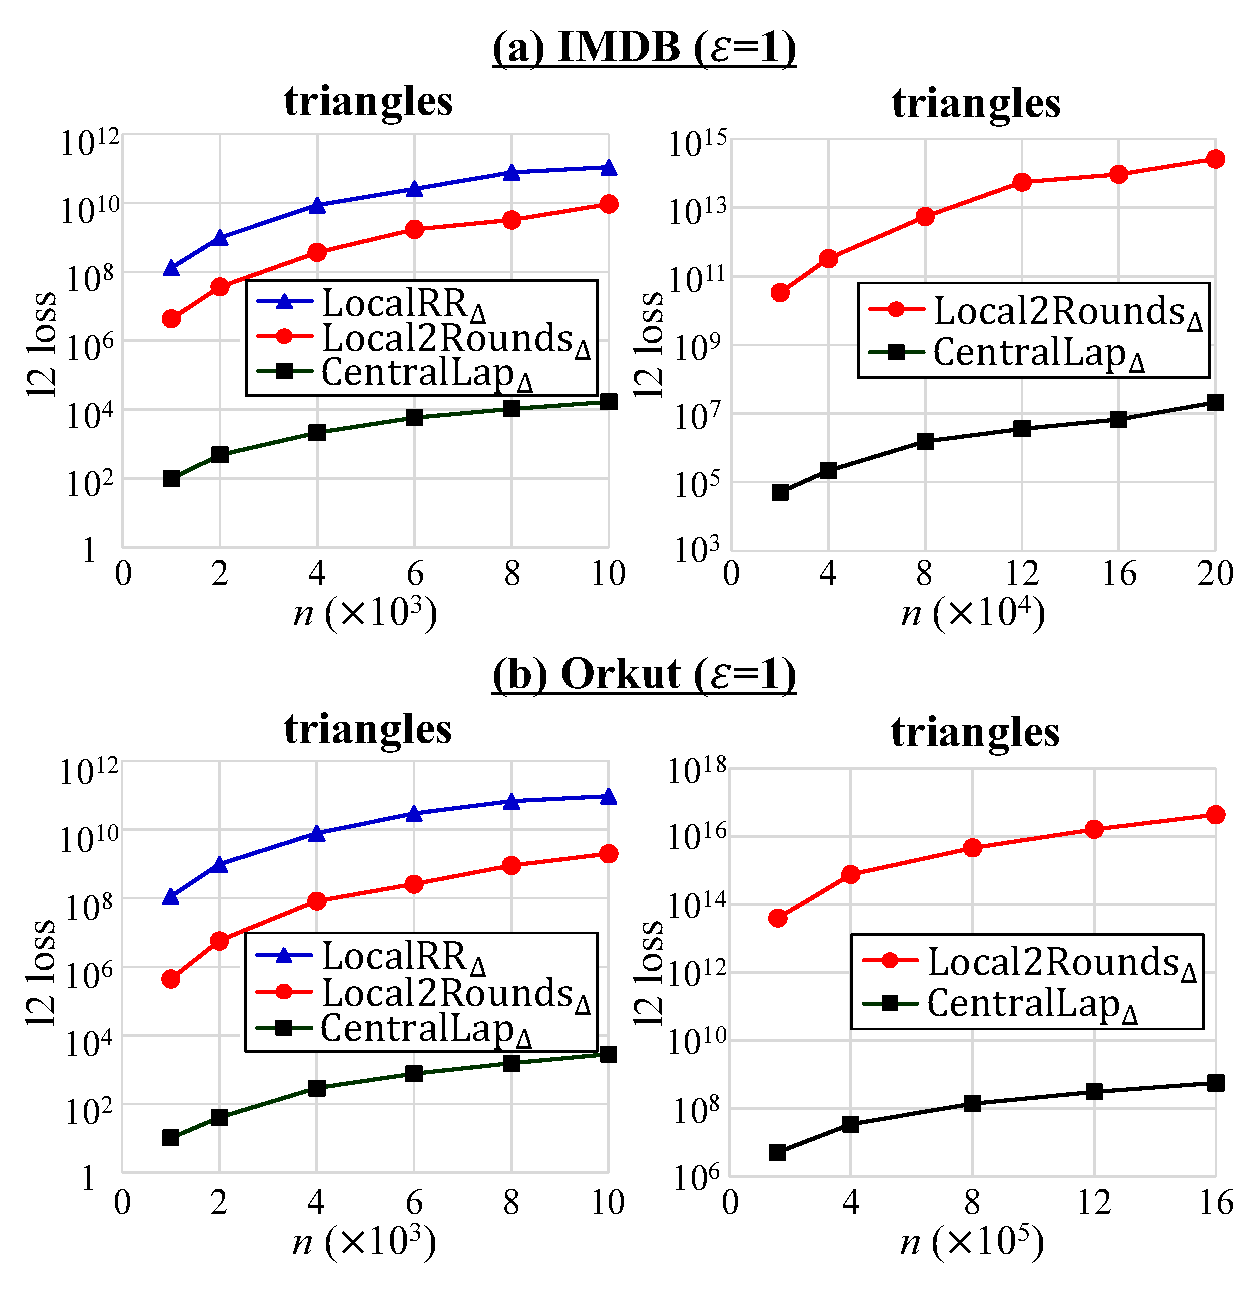
\includegraphics[width=0.99\linewidth]{fig/res1_n_l2loss_tri.pdf}
\vspace{-4mm}
\caption{Relation between the number of users $n$ and the $l_2$ loss in triangle counts when $\epsilon = 1$ ($\epsilon_1 = \epsilon_2 = \frac{1}{2}$, $\td_{max} = d_{max}$). 
Here we do not evaluate \alg{LocalRR$_\triangle$} when $n > 10000$, because it is inefficient (see Section~\ref{sub:two_rounds} ``Time complexity'').}
\label{fig:res1_n_l2loss_tri}
\end{figure}

\begin{figure}[t]
\centering
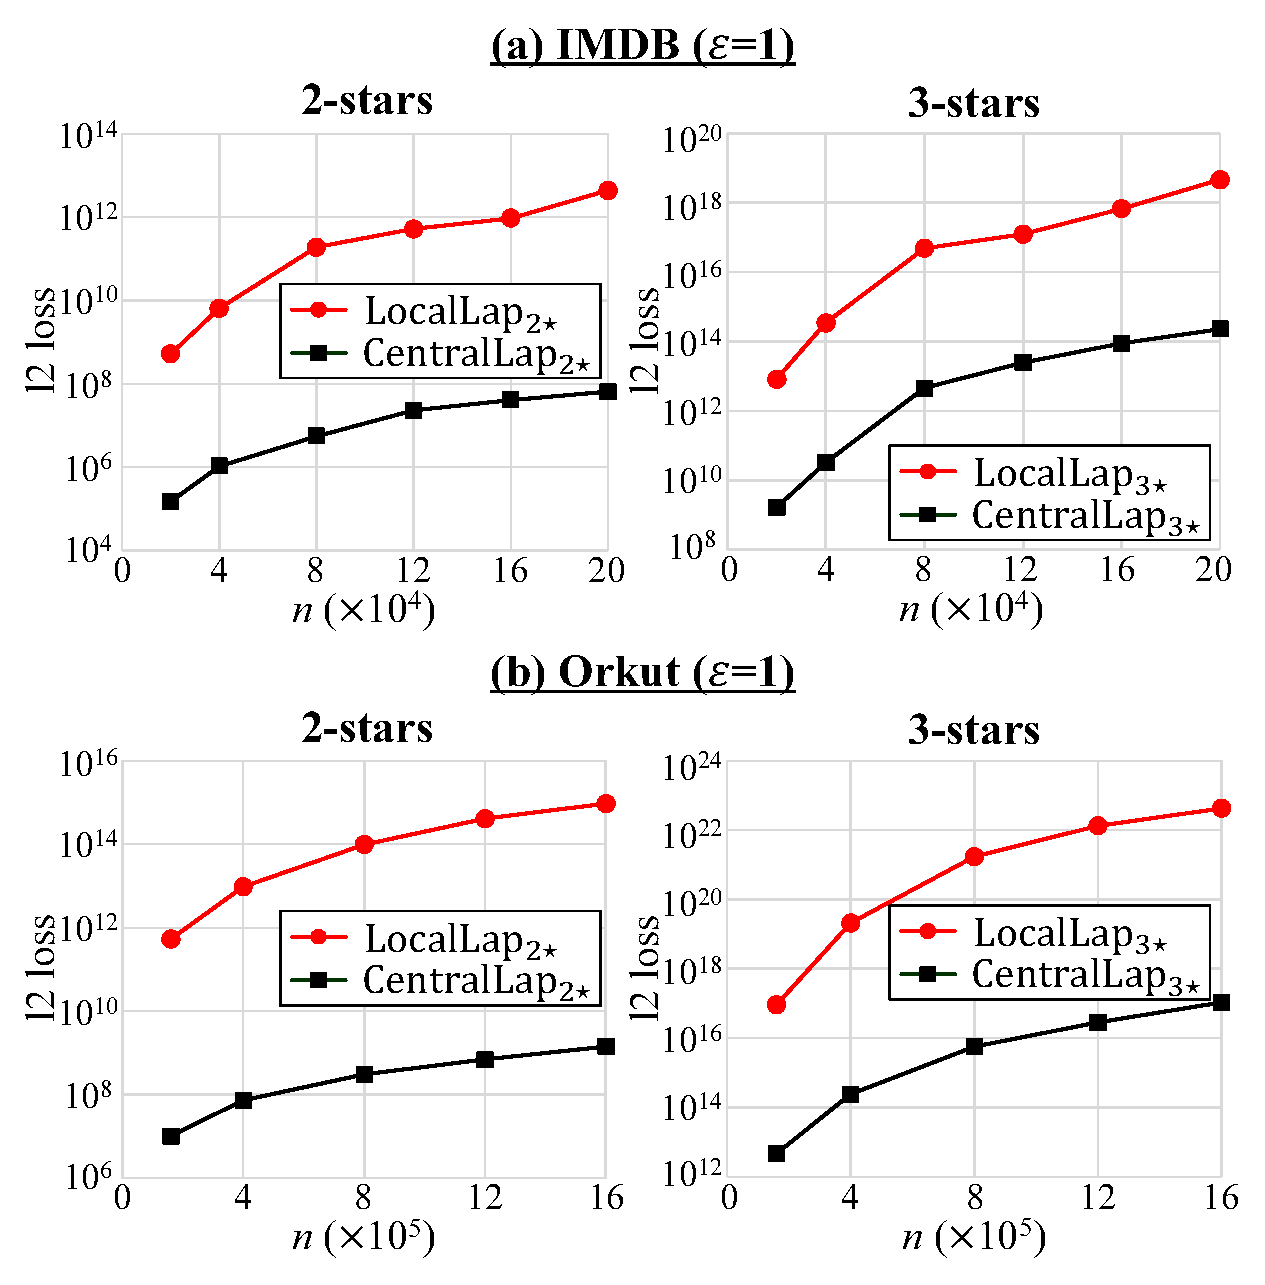
\includegraphics[width=0.99\linewidth]{fig/res1_n_l2loss_kst.pdf}
\vspace{-5mm}
\caption{Relation between the number of users $n$ and the $l_2$ loss in $k$-star counts when $\epsilon=1$ ($\epsilon_1 = \epsilon_2 = \frac{1}{2}$, $\td_{max} = d_{max}$).}
\label{fig:res1_n_l2loss_kst}
\end{figure}

\subsection{Experimental Results}
\label{sub:results}
\noindent{\textbf{Relation between $n$ and the $l_2$ loss.}}~~We first evaluated the $l_2$ loss of the estimates of 
% the numbers of triangles ($f_\triangle(G)$), $2$-stars ($f_{2\star}(G)$), and $3$-stars ($f_{3\star}(G)$), 
$f_\triangle(G)$, 
% (triangle counts), 
$f_{2\star}(G)$, 
% ($2$-star counts), 
and $f_{3\star}(G)$ 
% ($3$-star counts) 
while changing the number of users $n$. 
Figures~\ref{fig:res1_n_l2loss_tri} and \ref{fig:res1_n_l2loss_kst} shows the results ($\epsilon=1$). 
Here 
% we changed $n$ from $1000$ to $200000$ in \IMDB{}, and from $1000$ to $1600000$ in \Orkut{}. 
% Note that 
we did not evaluate \alg{LocalRR$_\triangle$} when $n$ was larger than $10000$, because \alg{LocalRR$_\triangle$} was inefficient 
% (the time complexity of \alg{LocalRR$_\triangle$} is $O(n^3)$, as described in Section~\ref{sub:two_rounds}). 
(as described in Section~\ref{sub:two_rounds} ``Time complexity''). 
% In Figures~\ref{fig:res1_n_l2loss_tri} and \ref{fig:res1_n_l2loss_kst}, 
In \alg{Local2Rounds$_\triangle$}, we set $\epsilon_1 = \epsilon_2 = \frac{1}{2}$. 
% so that $\epsilon = \epsilon_1 + \epsilon_2 = 1$. 
% In \alg{Local2Rounds$_\triangle$},  \alg{CentralLap$_\triangle$}, \alg{LocalLap$_k\star$}, and \alg{CentralLap$_k\star$}, 
As for $\td_{max}$, 
we set $\td_{max} = d_{max}$ (i.e., we assumed that $d_{max}$ is publicly available and did not perform graph projection) 
% , 
because we want to examine how well our theoretical results hold in our experiments. 
% we added the Laplacian noise with the local sensitivity in \alg{Proposal}, \alg{central (Lap)}, and \alg{local (Lap)}. 
We also evaluate the effectiveness of the private calculation of $d_{max}$ at the end of Section~\ref{sub:results}. 

Figure~\ref{fig:res1_n_l2loss_tri} shows that \alg{Local2Rounds$_\triangle$} significantly outperforms \alg{LocalRR$_\triangle$}. 
% for estimating $f_\triangle(G)$. 
Specifically, the $l_2$ loss of \alg{Local2Rounds$_\triangle$} is smaller than that of \alg{LocalRR$_\triangle$} by a factor of about $10^2$. 
% and $10^2 \sim 10^3$ in \IMDB{} and \Orkut{}, respectively. 
The difference between \alg{Local2Rounds$_\triangle$} and \alg{LocalRR$_\triangle$} is larger in \Orkut{}. 
This is because \Orkut{} is more sparse, as described in Section~\ref{sub:setup}. 
For example, when $n=10000$, the maximum degree $d_{max}$ in $G$ was $73.5$ and $27.8$ on average in \IMDB{} and \Orkut{}, respectively. 
Recall that for a fixed $\epsilon$, 
the expected $l_2$ loss of \alg{Local2Rounds$_\triangle$} and \alg{LocalRR$_\triangle$} 
can be expressed as $O(nd_{max}^3)$ and $O(n^4)$, respectively. 
Thus \alg{Local2Rounds$_\triangle$} significantly outperforms \alg{LocalRR$_\triangle$}, especially in sparse graphs. 
% datasets. 

% Figures~\ref{fig:res1_n_l2loss_tri} and \ref{fig:res1_n_l2loss_kst} show that \alg{central (Lap)} provides the best performance, which is consistent with our theoretical results; i.e., 

Figures~\ref{fig:res1_n_l2loss_tri} and \ref{fig:res1_n_l2loss_kst} show that the $l_2$ loss is roughly consistent with 
our upper-bounds in terms of $n$. 
Specifically, 
\alg{LocalRR$_\triangle$}, 
\alg{Local2Rounds$_\triangle$},  \alg{CentralLap$_\triangle$}, 
\alg{LocalLap$_{k\star}$}, and 
\alg{CentralLap$_{k\star}$} achieve 
the expected $l_2$ loss of $O(n^4)$, $O(nd_{max}^3)$, $O(d_{max}^2)$, $O(nd_{max}^{2k-2})$, and $O(d_{max}^{2k-2})$, respectively. 
Here note that 
% the maximum degree $d_{max}$ increases roughly in proportion to $n$ (though $d_{max}$ is much smaller than $n$), 
each user's degree increases roughly in proportion to $n$ (though the degree is much smaller than $n$), 
as we randomly select $n$ users from the whole graph $G^*$. Assuming that $d_{max} = O(n)$,  Figures~\ref{fig:res1_n_l2loss_tri} and \ref{fig:res1_n_l2loss_kst} are roughly consistent with the upper-bounds. 
The figures also show the limitations of the local model in terms of the utility when compared to the centralized model.

% when we increase $n$ by a factor of $10$, 
% the $l_2$ loss in triangle counts increases by a factor of about $10^4$, $10^4$, $10^2$ in \alg{LocalRR$_\triangle$}, \alg{Local2Rounds$_\triangle$}, and \alg{central (Lap)}, respectively. 
% Therefore, the experimental results are roughly consistent with our theoretical results that the expected $l_2$ loss of \alg{LocalRR$_\triangle$}, \alg{Local2Rounds$_\triangle$}, and \alg{CentralLap$_\triangle$} is $O(n^4)$, $O(nd_{max}^3)$, and $O(d_{max}^2)$, respectively. 
% The same applies to $k$-star counts. 

\smallskip
\noindent{\textbf{Relation between $\epsilon$ and the $l_2$ loss.}}~~Next we evaluated the $l_2$ loss 
% of the estimates of $f_\triangle(G)$ (triangle counts) and $f_{2\star}(G)$ ($2$-star counts), 
when we changed the privacy budget $\epsilon$ in edge LDP. 
Figure~\ref{fig:res2_eps_l2loss} shows the results for triangles and $2$-stars ($n=10000$). 
% (the result of $3$-stars is similar to that of $2$-stars, and therefore we omit the result of $3$-stars). 
Here we omit the result of $3$-stars because it is similar to that of $2$-stars. 
In \alg{Local2Rounds$_\triangle$}, we set $\epsilon_1 = \epsilon_2 = \frac{\epsilon}{2}$. 

Figure~\ref{fig:res2_eps_l2loss} shows that the $l_2$ loss is roughly consistent with 
% the expected $l_2$ loss in 
% our theoretical analysis 
our upper-bounds in terms of $\epsilon$. 
For example, when we decrease $\epsilon$ from $0.4$ to $0.1$, the $l_2$ loss 
% in triangle counts 
increases by a factor of about $5000$, $200$, and $16$ for both the datasets in \alg{LocalRR$_\triangle$}, \alg{Local2Rounds$_\triangle$}, and \alg{CentralLap$_\triangle$}, respectively. 
% This is 
They are 
roughly consistent with our theoretical results 
that for small $\epsilon$, the expected $l_2$ loss of \alg{LocalRR$_\triangle$}, \alg{Local2Rounds$_\triangle$}, and \alg{CentralLap$_\triangle$} is  $O(\epsilon^{-6})$\footnote{We used $e^\epsilon \approx \epsilon + 1$ to derive the upper-bound of \alg{LocalRR$_\triangle$} for small $\epsilon$.}, $O(\epsilon^{-4})$, and $O(\epsilon^{-2})$, respectively. 
% The same applies to large $\epsilon$ (e.g., $\epsilon = 1$ or $2$). 

\begin{figure}[t]
\centering
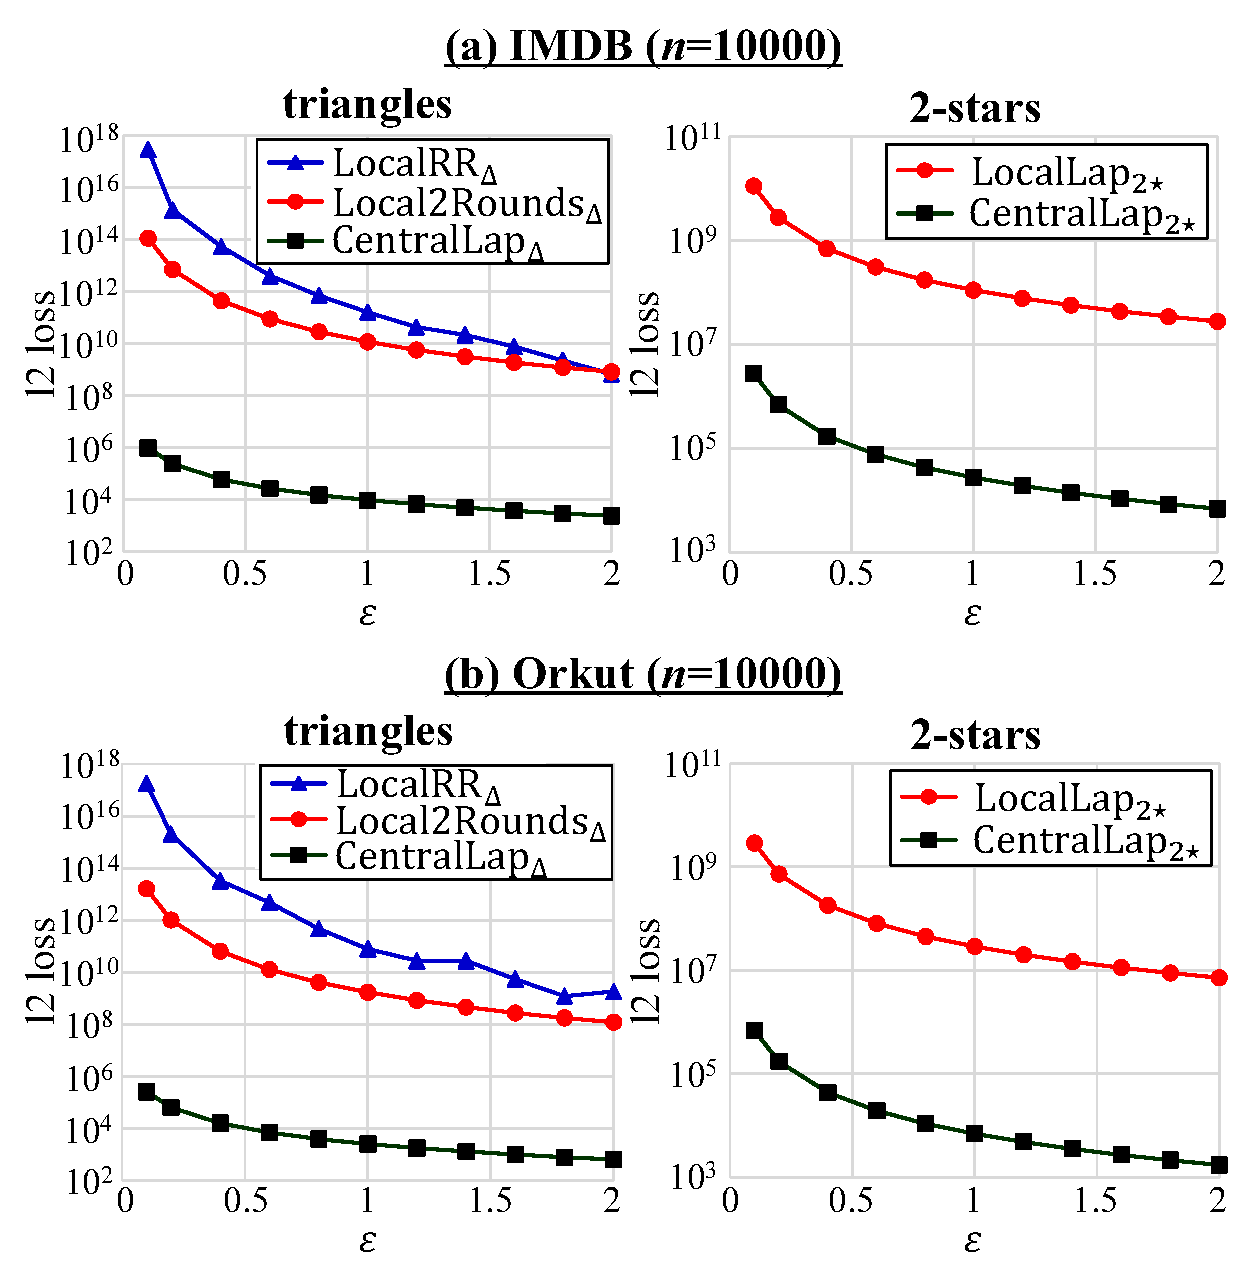
\includegraphics[width=0.99\linewidth]{fig/res2_eps_l2loss.pdf}
\vspace{-5mm}
\caption{Relation between $\epsilon$ in edge LDP and the $l_2$ loss when $n=10000$ ($\epsilon_1 = \epsilon_2 = \frac{\epsilon}{2}$, $\td_{max} = d_{max}$).}
\label{fig:res2_eps_l2loss}
\end{figure}

\begin{figure}[t]
\centering
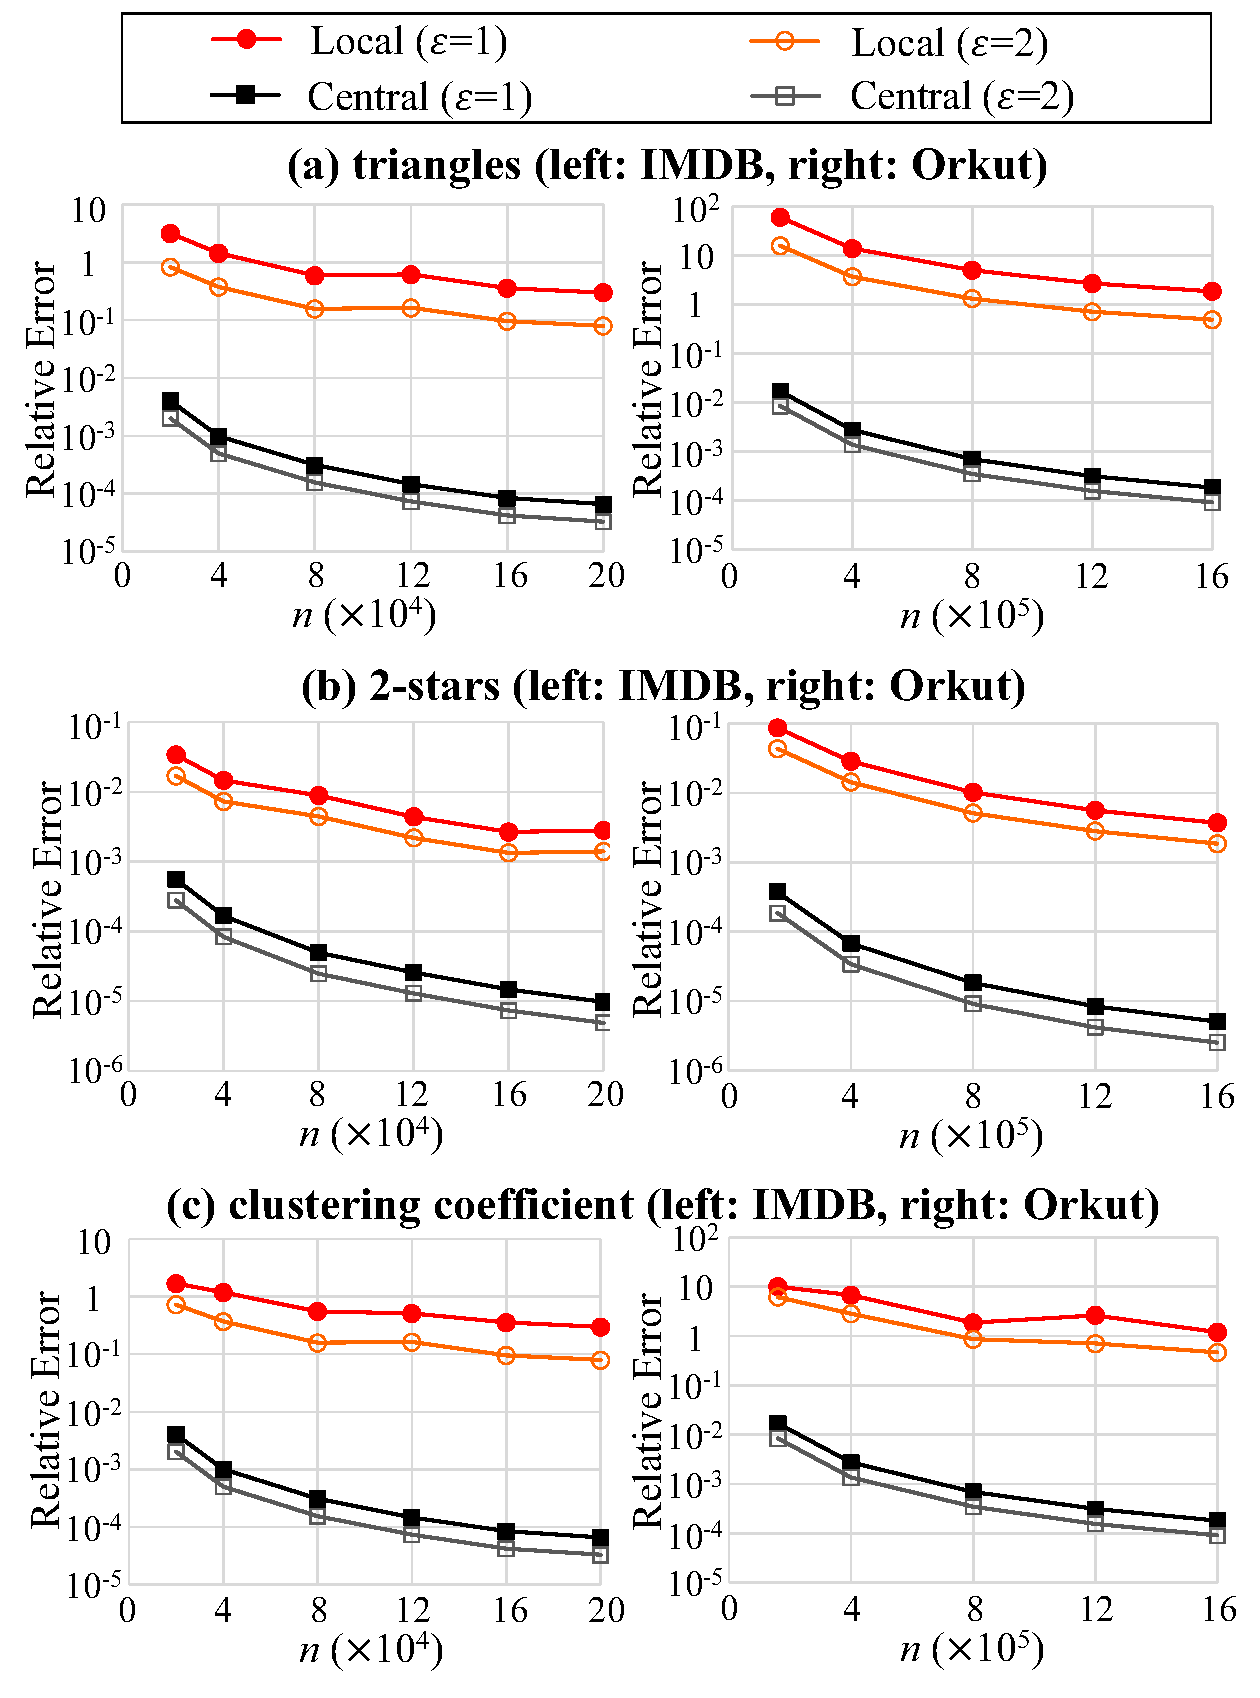
\includegraphics[width=0.99\linewidth]{fig/res3_n_relerr.pdf}
\vspace{-5mm}
\caption{Relation between 
% the number of users 
$n$ and the relative error. In the local model, we used \alg{Local2Rounds$_\triangle$} ($\epsilon = 1$ or $2$) and \alg{LocalLap$_k\star$} ($\epsilon = 1$ or $2$) for estimating triangle counts $f_\triangle(G)$ and $k$-star counts $f_{k\star}(G)$, respectively ($\td_{max} = d_{max}$).}
\label{fig:res3_n_relerr}
\end{figure}

Figure~\ref{fig:res2_eps_l2loss} also shows that 
\alg{Local2Rounds$_\triangle$} significantly outperforms \alg{LocalRR$_\triangle$} especially when $\epsilon$ is small, which is also consistent with our theoretical results. 
Conversely, the difference between \alg{LocalRR$_\triangle$} and \alg{Local2Rounds$_\triangle$} is small when $\epsilon$ is large. 
This is because when $\epsilon$ is large, the RR outputs the true value with high probability. 
For example, when 
% $\epsilon \geq 3$, 
$\epsilon \geq 5$, 
the RR outputs the true value with 
% $\frac{e^\epsilon}{e^\epsilon+1} > 0.95$. 
$\frac{e^\epsilon}{e^\epsilon+1} > 0.993$. 
% We also confirmed that when $\epsilon \geq 3$, the $l_2$ loss of \alg{LocalRR$_\triangle$} is smaller than \alg{Local2Rounds$_\triangle$} in both the datasets. 
However, \alg{LocalRR$_\triangle$} with 
% $\epsilon \geq 3$ 
such a large value of $\epsilon$ 
does not guarantee strong privacy, because it outputs the true value in most cases. 
% with more than $95\%$. 
\alg{Local2Rounds$_\triangle$} significantly outperforms \alg{LocalRR$_\triangle$} 
% for a reasonable range of $\epsilon$. 
when we want to estimate $f_\triangle(G)$ or $f_{k\star}(G)$ 
with a strong privacy guarantee; e.g., $\epsilon \leq 1$ \cite{DP_Li}. 

\smallskip
\noindent{\textbf{Relative error.}}~~As the number of users $n$ increases, the numbers of triangles $f_\triangle(G)$ and $k$-stars $f_{k\star}(G)$ increase. 
% , and this 
This causes the increase of the $l_2$ loss. 
Therefore, we also evaluated the relative error, as described in Section~\ref{sub:graph_statistics}. 

Figure~\ref{fig:res3_n_relerr} shows the relation between $n$ and the relative error 
(we omit the result of $3$-stars because it is similar to that of $2$-stars). 
In the local model, we used \alg{Local2Rounds$_\triangle$} and \alg{LocalLap$_k\star$} for estimating 
% triangle counts 
$f_\triangle(G)$ 
and 
% $k$-star counts, 
$f_{k\star}(G)$, 
respectively 
(we did not use \alg{Local2RR$_\triangle$}, because it is both inaccurate and inefficient). 
For both algorithms, we set $\epsilon = 1$ or $2$ 
($\epsilon_1 = \epsilon_2 = \frac{\epsilon}{2}$ in \alg{Local2Rounds$_\triangle$}) and $\td_{max} = d_{max}$. 
Then we estimated the clustering coefficient as: $\frac{3\hf_{\triangle}(G, \epsilon_1, \epsilon_2, d_{max})}{\hf_{k\star}(G, \epsilon, d_{max})}$, where 
$\hf_{\triangle}(G, \epsilon_1, \epsilon_2, d_{max})$ and 
$\hf_{k\star}(G, \epsilon, d_{max})$ are the estimates of $f_\triangle(G)$ and $f_{k\star}(G)$, respectively. 
If the estimate of the clustering coefficient is smaller than $0$ (resp.~larger than $1$), we set the estimate to $0$ (resp.~$1$) because the clustering coefficient is always between $0$ and $1$. 
In the centralized model, we used \alg{CentralLap$_\triangle$} and \alg{CentralLap$_k\star$} ($\epsilon=1$ or $2$, $\td_{max} = d_{max}$) and calculated the clustering coefficient in the same way. 

Figure~\ref{fig:res3_n_relerr} shows that for all cases, the relative error decreases with increase in $n$. 
This is because both $f_\triangle(G)$ and $f_{k\star}(G)$ significantly increase with increase in $n$. 
Specifically, let $f_{\triangle,v_i}(G) \in \nnints$ the number of triangles that involve user $v_i$, and $f_{k\star,v_i}(G) \in \nnints$ be the number of $k$-stars of which user $v_i$ is a center. 
Then $f_\triangle(G) = \frac{1}{3}\sum_{i=1}^n f_{\triangle,v_i}(G)$ and $f_{k\star,v_i}(G) = \sum_{i=1}^n f_{k\star,v_i}(G)$. 
Since both $f_{\triangle,v_i}(G)$ and $f_{k\star,v_i}(G)$ increase with increase in $n$, both $f_\triangle(G)$ and $f_{k\star}(G)$ increase \textit{at least} in proportion to $n$. 
Thus $f_\triangle(G)^2 \geq \Omega(n^2)$ and $f_{k\star}(G)^2 \geq \Omega(n^2)$. 
In contrast, \alg{Local2Rounds$_\triangle$}, \alg{LocalLap$_k\star$}, \alg{CentralLap$_\triangle$}, and \alg{CentralLap$_k\star$} achieve the expected $l_2$ loss of $O(n)$, $O(n)$, $O(1)$, and $O(1)$, respectively (when we ignore $d_{max}$ and $\epsilon$), all of which are smaller than $O(n^2)$. 
% the value $\frac{|\hf(G) - f(G)|}{|f(G)|}$ decreases with increase in $n$. 
% This explains the reason that 
Therefore, the relative error decreases with increase in $n$. 

This result demonstrates that we can accurately estimate graph statistics for large $n$ in the local model. 
In particular, the relative error is smaller in \IMDB{} 
% , 
because \IMDB{} is denser and includes a larger number of triangles and $k$-stars; i.e., the denominator of the relative error is large. 
For example, when $n=200000$ and $\epsilon=1$, the relative error is 
% $0.19$, 
$0.30$ and 
$0.0028$ 
% , and $0.015$ 
for triangles and $2$-stars, 
% , and $3$-stars, 
respectively. 
Note that the clustering coefficient requires $2\epsilon$ 
% , 
because we need to estimate both $f_\triangle(G)$ and $f_{k\star}(G)$. 
Yet, we can still accurately calculate the clustering coefficient with a moderate privacy budget; 
% $\epsilon$; 
e.g., the relative error of the clustering coefficient is 
%$0.19$ 
$0.30$ 
when the privacy budget is $2$ (i.e., $\epsilon = 1$).
If $n$ is larger, then $\epsilon$ would be smaller at the same value of the relative error. 

\begin{figure}[t]
\centering
% 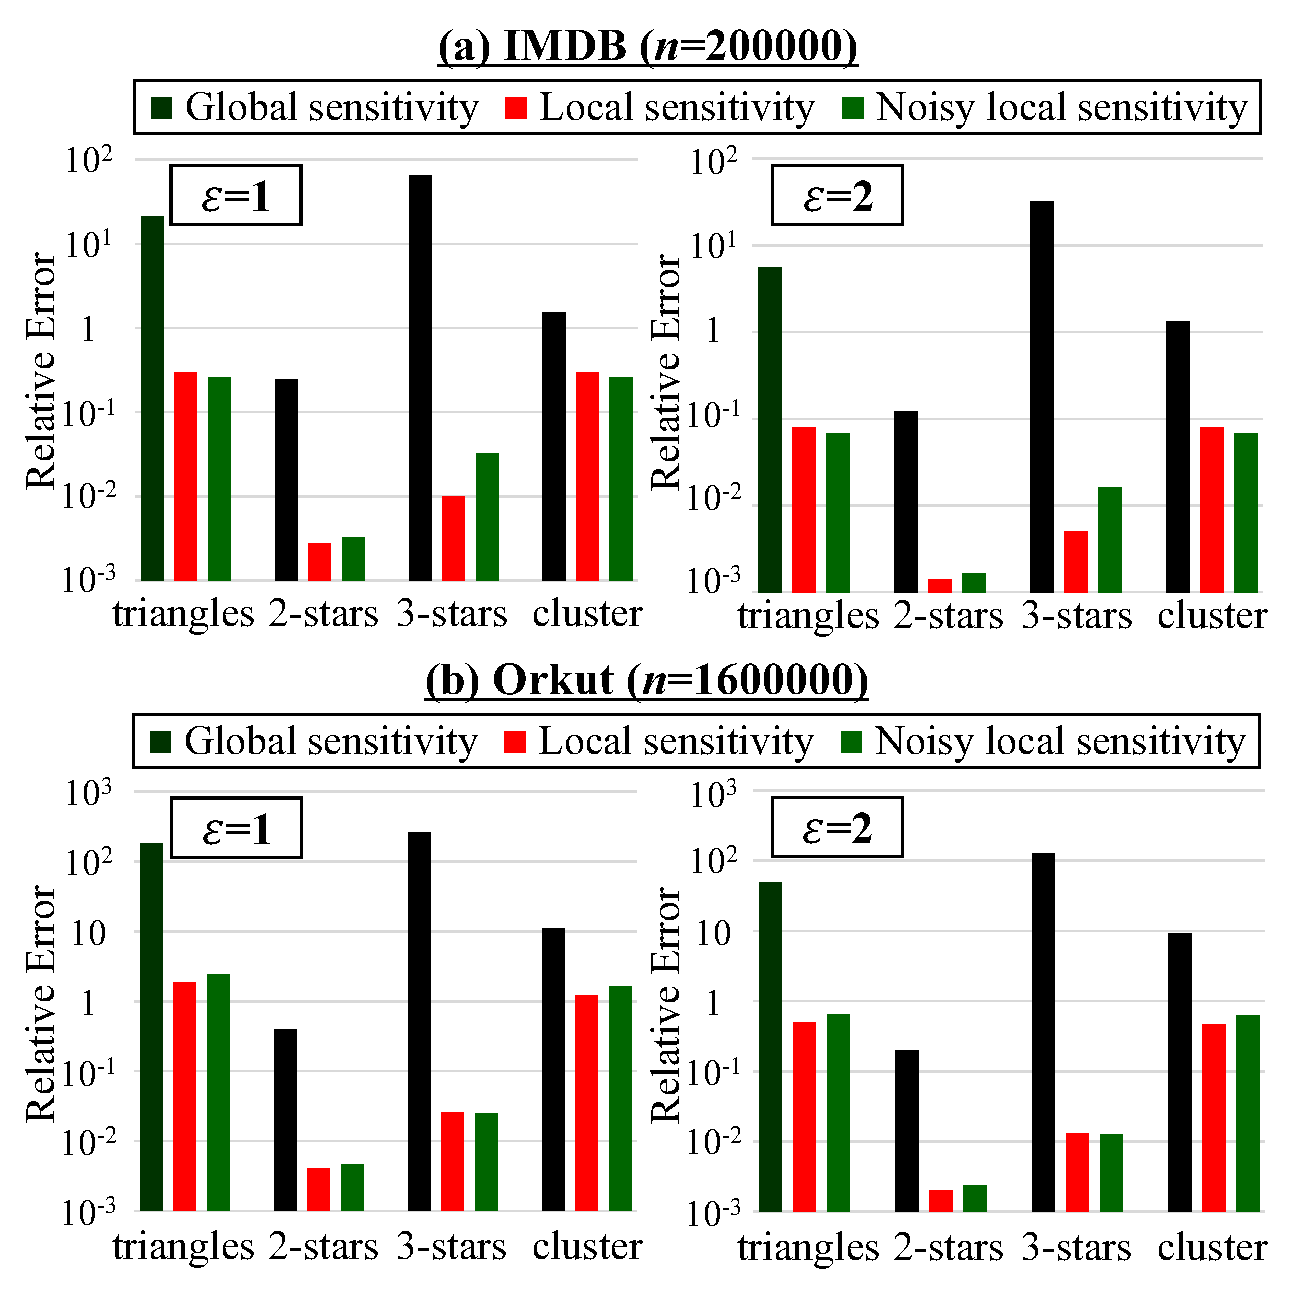
\includegraphics[width=0.99\linewidth]{fig/res4_noisy_local.pdf}
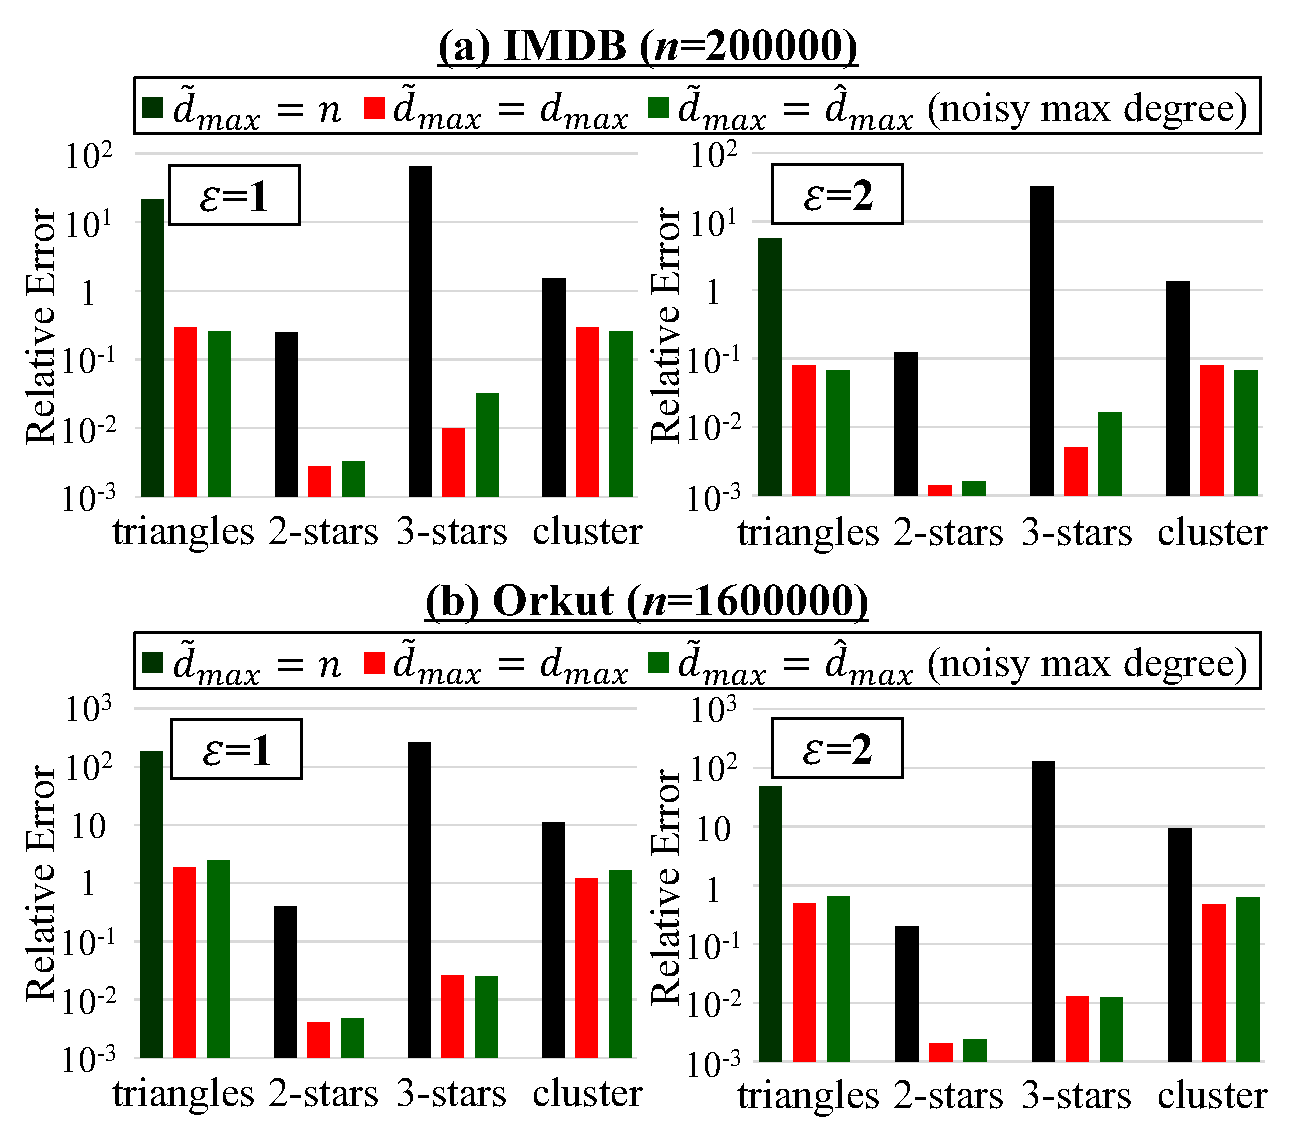
\includegraphics[width=0.99\linewidth]{fig/res4_noisy_max.pdf}
\vspace{-4mm}
\caption{Relative error 
% for 
% three types of sensitivity: 
% global sensitivity ($\td_{max} = n$), 
% local sensitivity ($\td_{max} = d_{max}$), and 
% noisy local sensitivity ($\td_{max} = \hd_{max}$). 
when $\td_{max} = n$ (\#users), 
$d_{max}$ (max degree), or 
$\hd_{max}$ (noisy max degree). 
% $\hd_{max}$ represents the private estimate of $d_{max}$; i.e., noisy max degree. 
We used \alg{Local2Rounds$_\triangle$} ($\epsilon = 1$ or $2$) and \alg{LocalLap$_k\star$} ($\epsilon = 1$ or $2$) for estimating triangle counts $f_\triangle(G)$ and $k$-star counts $f_{k\star}(G)$, respectively. 
% In ``Local sensitivity (Cauchy),'' we added the Cauchy noise (rather than the Laplacian noise) with the local sensitivity, which is always smaller than or equal to the smooth sensitivity \cite{Karwa_PVLDB11}.
}
\label{fig:res4_noisy_local}
\end{figure}

\smallskip
\noindent{\textbf{Private calculation of $d_{max}$.}}~~We have so far assumed that $\td_{max} = d_{max}$ (i.e., $d_{max}$ is publicly available) in our experiments. 
% However, it is difficult for the users and the data collector to know the exact value of $d_{max}$ in advance. 
% Therefore, we 
We 
finally evaluate the methods to privately calculate $d_{max}$ with $\epsilon_0$-edge LDP 
% , which are 
(described in Sections~\ref{sub:non-interactive_k_stars} and \ref{sub:two_rounds}). 
% show that even if we privately calculate $d_{max}$ with edge LDP, we can accurately estimate graph statistics in the local model. 

Specifically, we used \alg{Local2Rounds$_\triangle$} and \alg{LocalLap$_k\star$} for estimating $f_\triangle(G)$ and $f_{k\star}(G)$, respectively, and evaluated the following three methods for setting $\td_{max}$: 
% the sensitivity: 
% \begin{enumerate}
%     \item Set $\td_{max} = n$. We call this method the \textit{global sensitivity method} because it results in adding the Laplacian noise with the global sensitivity in Definition~\ref{def:global_sen}.
%     \item Set $\td_{max} = d_{max}$. We call this method the \textit{local sensitivity method} because it results in adding the Laplacian noise with the local sensitivity. 
% \end{enumerate}
(i) 
% set 
$\td_{max} = n$; 
(ii) 
% set 
$\td_{max} = d_{max}$; 
(iii) 
% set 
$\td_{max} = \hd_{max}$, where $\hd_{max}$ is the private estimate of $d_{max}$ 
% (i.e., 
(noisy max degree) in Sections~\ref{sub:non-interactive_k_stars} and \ref{sub:two_rounds}. 
% Note that the first (resp.~second) method results in adding the Laplacian noise with the global (resp.~local) sensitivity without using graph projection. 
% Therefore, we refer to the first method (i) as the \textit{global sensitivity method}, the second method (ii) as the \textit{local sensitivity method}, and the third method (iii) as the \textit{noisy local sensitivity method}. 

We set $n=200000$ in \IMDB{} and $n=1600000$ in \Orkut{}. 
Regarding the total privacy budget $\epsilon$ in edge LDP for estimating $f_\triangle(G)$ or $f_{k\star}(G)$, we set $\epsilon=1$ or $2$. 
We used $\frac{\epsilon}{10}$ for privately calculating $d_{max}$ (i.e., $\epsilon_0 = \frac{\epsilon}{10}$), and the remaining privacy budget $\frac{9\epsilon}{10}$ as input to \alg{Local2Rounds$_\triangle$} or \alg{LocalLap$_k\star$}. 
% estimating $f_\triangle(G)$ or $f_{k\star}(G)$. 
In \alg{Local2Rounds$_\triangle$}, we set $\epsilon_1 = \epsilon_2$; i.e., we set $(\epsilon_0, \epsilon_1, \epsilon_2) = (0.1, 0.45, 0.45)$ or $(0.2, 0.9, 0.9)$. 
% For example, \alg{Local2Rounds$_\triangle$} with $(\epsilon_0, \epsilon_1, \epsilon_2) = (0.1, 0.45, 0.45)$ provides $1$-edge LDP and $1.1$-entire edge LDP (see Section~\ref{sub:two_rounds}). 
Then we estimated the clustering coefficient in the same way as Figure~\ref{fig:res3_n_relerr}. 

Figure~\ref{fig:res4_noisy_local} shows the results. 
Figure~\ref{fig:res4_noisy_local} shows that 
% the noisy local sensitivity method 
the algorithms with $\td_{max} = \hd_{max}$ (noisy max degree) 
achieves the relative error close to (sometimes almost the same as) 
% the local sensitivity method, 
the algorithms with $\td_{max} = d_{max}$ 
and significantly outperforms 
% the global sensitivity method. 
the algorithms with $\td_{max} = n$. 
This means that we can privately estimate $d_{max}$ without a significant loss of utility. 
% Recall that the private calculation of $d_{max}$ does not increase the number of rounds in \alg{Local2Rounds$_\triangle$}. 
% Therefore, we can privately estimate $d_{max}$ and then accurately estimate all the graph statistics (i.e., triangles, $k$-stars, and the clustering coefficient) within two rounds.

\smallskip
\noindent{\textbf{Summary of results.}}~~In summary, 
% our experimental results were roughly consistent with our theoretical results. 
our experimental results showed that the estimation error of triangle counts is significantly reduced by introducing the interaction between users and a data collector. 
The results also showed that 
% we can accurately estimate graph statistics in the local model. 
% In particular, 
we can achieve small relative errors 
(much smaller than 1) for subgraph counts 
% for a large number of users $n$ 
with privacy budget $\epsilon=1$ or $2$ in edge LDP. 
% The results also showed that we can privately estimate the maximum degree $d_{max}$, which is required in both \alg{Local2Rounds$_\triangle$} and \alg{LocalLap$_k\star$}, without a significant loss of utility. 

As described in Section~\ref{sec:intro}, non-private 
% triangle or $k$-star 
subgraph 
counts may reveal some friendship information, and a central server may face data breaches. 
Our LDP algorithms are highly beneficial because they enable us to analyze the connection patterns in a graph 
(i.e., subgraph counts) 
or to understand how likely two friends of an individual will also be a friend 
% (which is useful for friend suggestion) 
(i.e., clustering coefficient) 
while strongly protecting individual privacy.


\section{Conclusions}
\label{chap1-sec:conclusions}
% In this paper, 
We presented a series of algorithms for counting triangles and $k$-stars under LDP. 
We 
% analyzed the upper-bounds on the expected $l_2$ loss for these algorithms, and 
showed that an additional round can significantly reduce the estimation error in triangles, and the algorithm based on the Laplacian mechanism provides an order optimal error in the non-interactive local model. 
We also showed lower-bounds for general functions including triangles and $k$-stars. 
We conducted experiments using two real datasets, and showed that our algorithms achieve small relative errors, especially when the number of users is large.

As future work, we would like to develop algorithms for other subgraph counts such as cliques and $k$-triangles \cite{Karwa_PVLDB11}. 

% %-------------------------------------------------------------------------------
\section*{Acknowledgments}
Kamalika Chaudhuri and Jacob Imola would like to thank ONR under N00014-20-1-2334 and UC Lab Fees under LFR 18-548554  for research support. 
Takao Murakami was supported in part by JSPS KAKENHI JP19H04113.



\graphicspath{{./chapters/chapter2/}}

\chapter{Communication-Efficient Triangle Counting under Local Differential Privacy}

%\newcommand{\nats}{\mathbb{N}}
%\newcommand{\nnints}{\mathbb{Z}_{\ge0}}
%\newcommand{\reals}{\mathbb{R}}
%\newcommand{\nnreals}{\mathbb{R}_{\ge0}}
%\newcommand{\argmax}{\operatornamewithlimits{argmax}}
%\newcommand{\argmin}{\operatornamewithlimits{argmin}}

\def\bd{\bar{d}}
\def\bbma{\bar{\bma}}
\def\hd{\hat{d}}
\def\hf{\hat{f}}
\def\hg{\hat{g}}
\def\hr{\hat{r}}
\def\hw{\hat{w}}
\def\td{\tilde{d}}
% \def\AlgOne{\textsf{PrivSampleFullDwnld}$_{\triangle}$}
% \def\AlgTwo{\textsf{PrivSampleHalfNoisyDwnld}$_{\triangle}$}
% \def\AlgThree{\textsf{PrivSampleBothNoisyDwnld}$_{\triangle}$}
% \def\AlgOne{\textsf{ARRFullDL}$_{\triangle}$}
% \def\AlgTwo{\textsf{ARROneNoisyDL}$_{\triangle}$}
% \def\AlgThree{\textsf{ARRTwoNoisyDL}$_{\triangle}$}
% \def\AlgSec{\textsf{RRFullDL}$_{\triangle}(d_{max})$}
\def\AlgOne{\textsf{ARRFull}$_{\triangle}$}
\def\AlgTwo{\textsf{ARROneNS}$_{\triangle}$}
\def\AlgThree{\textsf{ARRTwoNS}$_{\triangle}$}
\def\AlgSec{\textsf{RRFull}$_{\triangle}(d_{max})$}
\newcommand{\GPlus}{\textsf{Gplus}}
\newcommand{\CostDL}{\mathrm{Cost}_{DL}}
\newcommand{\CostUL}{\mathrm{Cost}_{UL}}


\section{Introduction}
\label{chap2-sec:intro}
Counting subgraphs (e.g., triangles, stars, cycles) is
% a fundamental task 
one of the most basic tasks 
for analyzing connection patterns
% for analyzing graph statistics
in
% a graph.
various graph data, e.g., social,
communication, and collaboration networks.
% , epidemiological networks.
% Graph statistics is important to understand the connection patterns in various graph data; e.g., social networks, collaboration networks,
% For example, a degree distribution in a social graph represents a distribution of the number of friends in the graph.
% A subgraph count (e.g.,
For example,
% a triangle count is the number of three nodes with three edges.
% A $k$-star count is the number of a node connected to $k$ other nodes.
a triangle is given by a set of three nodes with three edges, whereas a $k$-star is given by a central node connected to $k$ other nodes.
% a set of $k$ nodes connected a central node.
These subgraphs
% are important because they can be used to calculate
play a crucial role in calculating
a \textit{clustering coefficient} ($=\frac{3 \times \text{\#triangles}}{\text{\#2-stars}}$) (see Figure~\ref{chap2-fig:triangles_stars}). 
% which 
The clustering coefficient 
measures the average probability that
two friends of a user will also be a friend
% a friend's friend is also a friend
in a social graph \cite{Newman_PRL09}. 
Therefore, it is useful for measuring the effectiveness of friend suggestions. 
In addition, the clustering coefficient represents the degree to which users tend to cluster together. 
Thus, if it is large in some services/communities, we can effectively apply social recommendations \cite{Kolluri_CCS21} to the users. 
% for an example of
% the triangle and $k$-star counts and clustering coefficient).
% these subgraph counts).
% \cite{Newman_PRL09}.
% It is also known that these subgraphs are sufficient statistics for exponential random graph models
Triangles 
and $k$-stars 
% can also be used for
are also useful for 
% modeling graphs \cite{Jorgensen_SIGMOD16,Robins_SN07}.
% generating graphs based on some
constructing
graph models
\cite{Robins_SN07,Jorgensen_SIGMOD16}; 
% and other applications \cite{Imola_USENIX21}.
% (e.g., exponential random graph models \cite{Robins_SN07}, TriCycle \cite{Jorgensen_SIGMOD16}).
% Applications of triangle counting are summarized in \cite{Tsourakakis_JGAA11}. 
see also \cite{Tsourakakis_JGAA11} for other applications of triangle counting. 
However, graph data often involve sensitive data such as sensitive edges (friendships),
% that a user wants to keep secret,
% which 
and they 
can be leaked from 
% exact values of triangle counts and $k$-star counts \cite{Imola_USENIX21}.
exact numbers of triangles and $k$-stars \cite{Imola_USENIX21}.
% Therefore,
% there is a need for
% we need to develop an algorithm for
% counting
% subgraphs while strongly protecting user privacy.
% , which is the focus of this paper.


To analyze subgraphs while protecting user privacy, DP (Differential Privacy) \cite{DP} has been widely adopted as a privacy metric \cite{Ding_TKDE21,Imola_USENIX21,Karwa_PVLDB11,Sun_CCS19,Ye_ICDE20,Ye_TKDE21,Zhang_SIGMOD15}.
DP protects user privacy against adversaries with arbitrary background knowledge and is known as a gold standard for data privacy.
% Most studies on private graph analysis \cite{Chen_PoPETs20,Day_SIGMOD16,Hay_ICDM09,Karwa_PVLDB11,Kasiviswanathan_TCC13,Nissim_STOC07,Raskhodnikova_arXiv15,Song_arXiv18} assumes central DP
According to the underlying model, DP can be categorized into \textit{central (or global) DP} and \textit{LDP (Local DP)}.
Central DP assumes a scenario where
% that
a central server has personal data of all users.
% whereas LDP does not assume such trusted servers.
Although accurate analysis of subgraphs is possible under
% central DP
this model \cite{Ding_TKDE21,Karwa_PVLDB11,Zhang_SIGMOD15}, there is a risk that the entire graph is leaked from the server by illegal access or internal fraud \cite{data_breach2021,CambridgeAnalytica}.
In addition, central DP cannot be applied to  \textit{decentralized social networks} 
\cite{Diaspora,Mastodon,Minds,Paul_CN14} 
% \cite{Diaspora,Mastodon,Paul_CN14} 
% (e.g., Diaspora \cite{Diaspora}, Mastodon \cite{Mastodon}) 
% which has no central server that has the entire graph, and uses many servers each of which has personal data of users who have registered
where the entire graph is distributed across many servers. 
% nor 
We can even consider 
\textit{fully decentralized applications} where a server does not have
any original edge, 
% between users, 
% information about the original edges;
% For example,
% mobile application in which each user sends the number of her friends
e.g., a mobile app that sends a noisy degree (noisy number of friends) to the server, which then estimates a degree distribution. 
Central DP cannot be used in such applications. 

In contrast, LDP assumes a scenario where each user obfuscates her personal data (friends list in 
the case of graphs) 
% data) 
by herself and sends the obfuscated data to a possibly malicious server; i.e., it does not assume trusted servers.
Thus, it does not suffer from a data breach and can also be applied to the decentralized applications. 
% explained above.
% LDP does not assume trusted servers, hence
% can be applied to the above decentralized applications.
% In LDP, each user obfuscates her personal data (friends list in the case of graph data) by herself, and sends the obfuscated data to a (possibly malicious) server.
% Since the server does not have the original data, it does not suffer from the data breach.
LDP has been widely studied in tabular data where each row corresponds to a user's personal data (e.g., age, browser setting, location) 
\cite{Acharya_AISTATS19,Bassily_NIPS17,Erlingsson_CCS14,Kairouz_ICML16,Murakami_USENIX19,Wang_USENIX17} 
% \cite{Acharya_AISTATS19,Bassily_NIPS17,Erlingsson_CCS14,Fanti_PoPETs16,Kairouz_ICML16,Murakami_USENIX19,Qin_CCS16,Wang_USENIX17}, 
and also in graph data \cite{Imola_USENIX21,Qin_CCS17,Ye_ICDE20,Ye_TKDE21}.
For example, $k$-star counts can be very accurately estimated under LDP because each user can count $k$-stars of which she is a center and sends a noisy version of her $k$-star count to the server \cite{Imola_USENIX21}.

However, more complex subgraphs such as triangles are much harder to count under LDP because each user
% is not aware of
cannot see
edges between other users.
For example, in Figure~\ref{chap2-fig:triangles_stars}, user $v_1$ cannot see
% an edge between $v_2$ and $v_3$,
edges between $v_2$, $v_3$, and $v_6$ 
and therefore 
% , hence 
cannot count triangles involving $v_1$.
Thus,
% when only one-round interaction is allowed between each user and the server,
% instead of sending a noisy triangle count,
existing algorithms \cite{Imola_USENIX21,Ye_ICDE20,Ye_TKDE21}
% send noisy edges (rather than noisy triangle counts) obtained by randomized response \cite{Warner_JASA65} to a server.
obfuscate each user's edges (rather than her triangle count) by
% Warner's
RR (Randomized Response)
% randomized response
\cite{Warner_JASA65} and send noisy edges to a server.
% , which then estimates the triangle count.
% \cite{Imola_USENIX21,Ye_ICDE20,Ye_TKDE21} apply Warner's RR (Randomized Response) \cite{Warner_JASA65}, which flips 0/1 with some probability, to each edge and then estimate the triangle count.
Consequently, the server suffers from a
% very
prohibitively
large estimation error
% as shown in \cite{Imola_USENIX21} and Appendix~\ref{chap2-sec:one-round} in our paper 
(e.g., relative error $> 10^2$ in large graphs, 
as shown in Appendix~\ref{chap2-sec:one-round}) 
% (e.g., relative error $> 10^2$ in large graphs, as shown in Appendix~\ref{chap2-sec:one-round} of our paper)
because all three edges are noisy in any noisy triangle the server sees.

\begin{figure}[t]
  \centering
  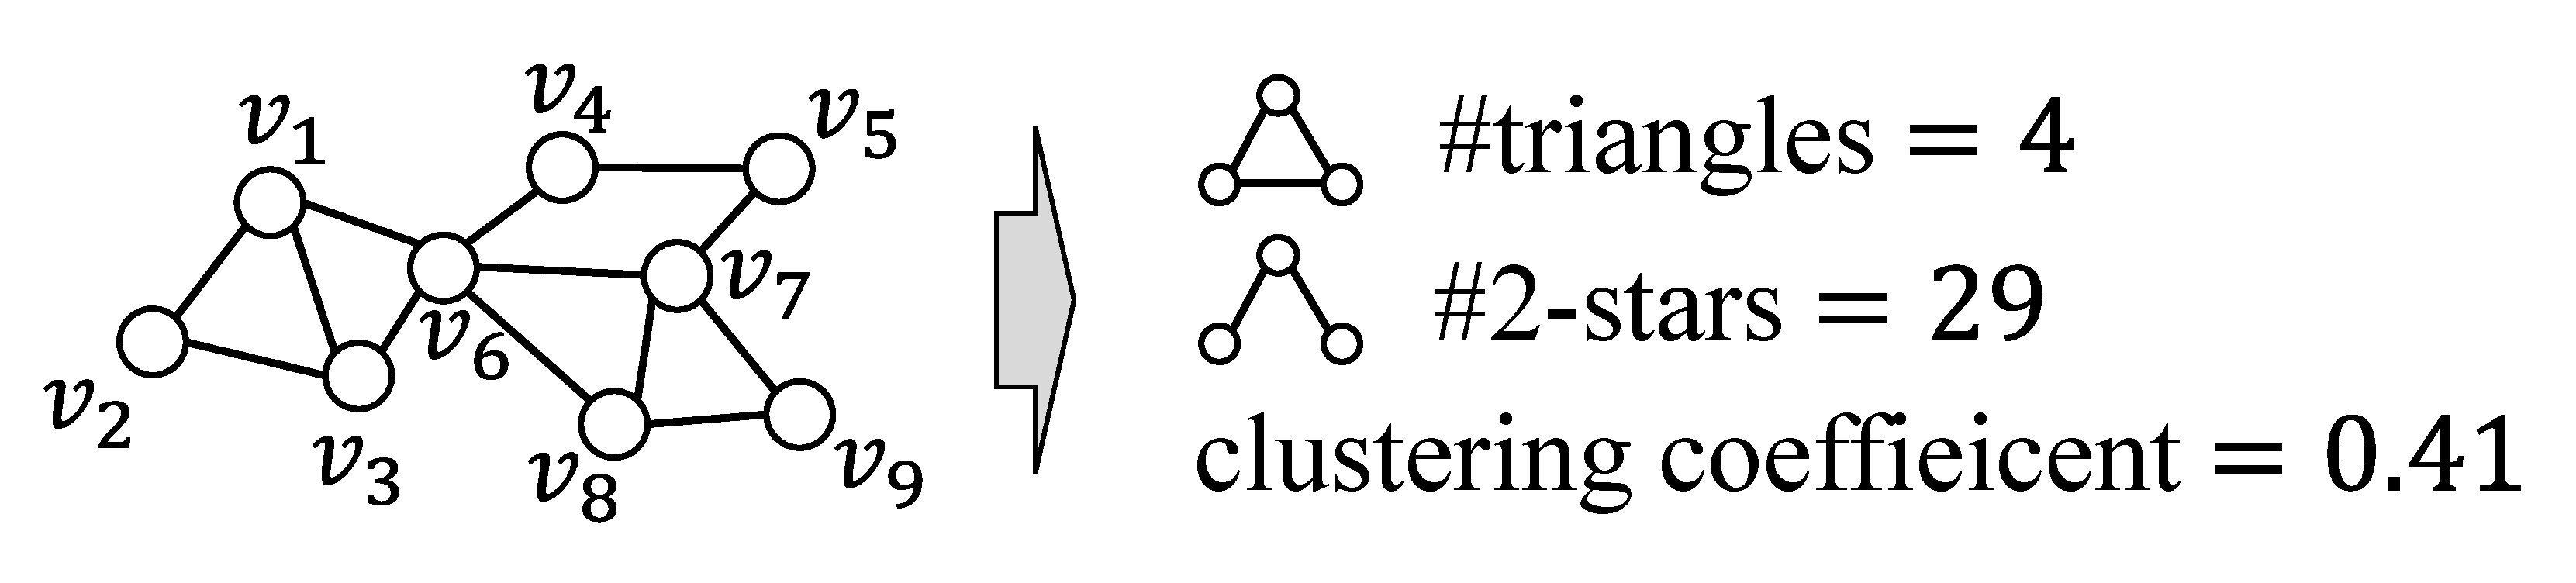
\includegraphics[width=0.85\linewidth]{fig/triangles_stars.pdf}
  
  \caption{Triangles, $2$-stars, and clustering coefficient.}
  \label{chap2-fig:triangles_stars}
\end{figure}

A recent study \cite{Imola_USENIX21} shows that the estimation error in
% triangle counting under LDP
locally private triangle counting
is significantly reduced by introducing an additional round of interaction between users and the server.
Specifically, if the server publishes the noisy graph (all noisy edges) sent by users at the first round, then each user can count her noisy triangles such that \textit{only one edge} is noisy (as she knows two edges connected to her).
Thus,
% each user
the algorithm in \cite{Imola_USENIX21} sends each user's noisy triangle count (with additional noise) to the server at the second round.
Then the server can accurately estimate the triangle count. 
% between users and the server 
% The algorithm in \cite{Imola_USENIX21} 
This algorithm also requires a much smaller number of interactions 
% between users and the server 
(i.e., only two) than collaborative approaches \cite{Kairouz_FTML21,Shokri_CCS15} that generally require many interactions. 

Unfortunately, 
% this algorithm 
the algorithm in \cite{Imola_USENIX21} 
is still
% far from practical
impractical 
for a large-scale graph.
% as shown in this paper.
Specifically, the noisy graph sent by users is dense, hence extremely large for a large-scale graph, e.g.,
$500$
% $400$
Gbits for a graph of
% about $900000$ users, as in our experiments).
a million users.
The problem is that \textit{every user} needs to download such huge data; e.g., when the download speed is $20$ Mbps (which is a recommended speed in YouTube \cite{YouTube_speed}), every user needs about 7 hours to download the noisy graph.
Since the communication ability might be limited for some users, the algorithm in \cite{Imola_USENIX21} cannot be
% applied to
used for
% a large-scale graph with diverse communication environments.
applications with large and diverse users.

In summary, existing triangle algorithms under LDP suffer from either a prohibitively large estimation error or a prohibitively 
% large 
high 
communication cost.
% For the same reason, they cannot calculate the clustering coefficient
They also suffer from the same issues when calculating the clustering coefficient.

% \colorB{
% \begin{itemize}
%     \item graph statistics; e.g., degree distribution, subgraph count (e.g., 2-stars, triangles), clustering coefficient.
%     \item privacy issue, DP, central DP, LDP.
%     \item 2-star counting under LDP is easy because...
%     \item triangle counting (hence clustering coefficient) is much harder because...
%     \item Previous work \cite{Imola_USENIX21}. Communication cost is prohibitively large (e.g., 400 Gbits for \IMDB{}).
%     \item This work
% \end{itemize}}

\smallskip
\noindent{\textbf{Our Contributions.}}~~We 
% In this work, we 
propose locally private triangle counting algorithms with a small estimation error and small communication cost.
% dramatically reduce the communication cost in accurate two-rounds triangle counting under LDP
% introduce some novel algorithms
% dramatically reduce the communication cost in locally private triangle counting
% address this issue
% by introducing some novel algorithms.
% Specifically, our contributions are:
Our contributions are as follows:

\begin{itemize}
    \item We propose two-rounds triangle algorithms
% that sample edges and then select edges each user downloads.
consisting of \textit{edge sampling} after RR and \textit{selecting edges each user downloads}.
In particular, we show that a simple extension of \cite{Imola_USENIX21} with edge sampling suffers from a large estimation error for a large or dense graph where the number of 4-cycles (such as $v_1$-$v_2$-$v_3$-$v_6$-$v_1$
% and $v_4$-$v_5$-$v_7$-$v_6$-$v_4$
in Figure~\ref{chap2-fig:triangles_stars}) is large.
To address this issue, we propose some strategies for selecting edges to download to reduce the error caused by the 4-cycles, which we call the \textit{4-cycle trick}.
\item We
show that
% the above algorithms
the algorithms with the $4$-cycle trick
still suffer from a large estimation error due to
% a large global sensitivity
% a large amount of the Laplacian noise.
large Laplacian noise for each user.
% To address this, 
To significantly reduce the Laplacian noise, 
we
propose a \textit{double clipping} technique,
which clips 
a degree (the number of edges) of each user 
% the number of edges 
with LDP and then clips the number of noisy triangles. 
% to significantly reduce the Laplacian noise.
% which significantly reduces the Laplacian noise by edge clipping and noisy triangle clipping.
% consists of edge clipping and noisy triangle clipping, to significantly reduce the global sensitivity in DP \cite{DP}.
% consisting of edge clipping and noisy triangle clipping
\item We evaluate our algorithms using two real datasets.
We show that our entire algorithms with the 4-cycle trick and double clipping
% provide the best performance, and
dramatically reduce the communication cost
% when compared with
of
\cite{Imola_USENIX21}.
For example,
% when the number of users is about $900000$,
for a graph with about $900000$ users,
we reduce the download cost from $400$ Gbits ($6$ hours when $20$ Mbps) to 
% $100$ Mbits ($5$ seconds) 
$160$ Mbits ($8$ seconds) or less 
while keeping the relative error much smaller than 1.
\end{itemize}
Thus, locally private triangle counting is now much more practical. 
% Note that the number of interactions between users and a server in our algorithms (i.e, only two) is also much smaller than collaborative approaches that generally requires a number of interactions. 
In Appendix~\ref{chap2-sec:cluster}, we also show that we can estimate the clustering coefficient with a small estimation error and download cost. 
For example, our algorithms are useful for measuring the effectiveness of friend suggestions or social recommendations in decentralized 
social networks, 
% SNS, 
e.g., Diaspora \cite{Diaspora}, Mastodon \cite{Mastodon}. 
% We published
Our source code
% with C/C++
is available at 
\cite{TriangleLDP}. 
%\cite{ComTriLDP}.
% as open-source software.

All the proofs of our privacy and utility analysis 
% The proofs of all statements 
are given in \conference{the full version \cite{Imola_arXiv22}}\arxiv{Appendices~\ref{chap2-sec:proof_seq_comp_edge_LDP}, \ref{chap2-sec:proof_algorithms}, and \ref{chap2-sec:proof_double_clip}}.

\smallskip
\noindent{\textbf{Technical Novelty.}}~~Below we explain more about 
% also clarify 
the technical novelty of this paper. 
Although we focus on two-rounds local algorithms in the same way as \cite{Imola_USENIX21}, we introduce several new algorithmic ideas previously unknown in the literature. 

First, our 4-cycle trick is totally new. 
Although some studies focus on 4-cycle counting \cite{Bera_STACS17,Kallaugher_PODS19,Manjunath_ESA11,McGregor_PODS20}, this work is the first to use 4-cycles to improve communication efficiency. 
Second, selective download of parts of a centrally computed quantity is also new. 
This is not limited to graphs -- even in machine learning, 
% or federated learning, 
there are no such strategic download techniques previously, to our knowledge. 
Third, our utility analysis of our 
% two-rounds 
triangle 
algorithms (Theorem~\ref{chap2-thm:l2loss_algorithms}) is 
% also now because it 
different from \cite{Imola_USENIX21} in that ours introduces subgraphs such as 4-cycles and $k$-stars. 
This leads us to our 4-cycle trick. 
Fourth, we propose two triangle algorithms that introduce the 4-cycle trick and show that the more tricky one provides the best performance because of 
its low sensitivity in DP.
% small Laplacian noise. 

% Fourth, 
Finally, 
our double clipping is new. 
Andrew \textit{et al.} \cite{Andrew_NeurIPS21} propose an adaptive clipping technique, which applies clipping twice. 
However, they focus on federated averaging, 
% or SGD (Stochastic Gradient Descent), 
and their problem setting is different from our graph setting. 
In particular, they require a private quantile of the norm distribution. 
In contrast, we need only a much simpler estimate: a private degree. 
Here, we use the fact that the degree has a small sensitivity (sensitivity $=1$) in DP for edges. 
We also provide a new, reasonably tight bound on the probability that the noisy triangle count exceeds a clipping threshold (Theorem~\ref{chap2-thm:triangle_excess}). 
Thanks to the two differences, we obtain a significant communication improvement: two or three orders of magnitude. 

% Finally, we show an interesting finding when we combine the 4-cycle trick and double clipping. 
% Specifically, we propose two triangle algorithms that introduce the 4-cycle trick and show that the more tricky one provides the best performance because of its low sensitivity.

\section{Related Work}
\label{chap2-sec:related}
% !TEX root=main.tex
\noindent{\textbf{Triangle Counting.}}~~Triangle
% We finally note that triangle
counting has been extensively studied in a non-private setting \cite{Bera_KDD20,Bera_PODS20,Chu_KDD11,Eden_FOCS15,Seshadhri_SDM13,Suri_WWW11,Tsourakakis_KDD09,Wu_TKDE16} 
% \cite{Arifuzzaman_CIKM13,Bera_KDD20,Bera_PODS20,Chu_KDD11,Eden_FOCS15,Kolountzakis_IM12,Seshadhri_SDM13,Suri_WWW11,Tangwongsan_CIKM13,Tsourakakis_KDD09,Wu_TKDE16}
(it is almost a sub-field in itself)
because it requires high time complexity for large graphs.

Edge sampling \cite{Bera_PODS20,Eden_FOCS15,Tsourakakis_KDD09,Wu_TKDE16} is one of the most basic techniques to improve 
% the 
scalability.
Although edge sampling is simple, it is quite effective -- it is reported in \cite{Wu_TKDE16} that edge sampling outperforms other sampling techniques such as node sampling and triangle sampling.
Based on this, we adopt edge sampling after RR\footnote{We also note that a study in \cite{Nguyen_TDP16} proposes a graph publishing algorithm in the central model that independently changes 1-cells (edges) to 0-cells (no edges) with some probability and then 
changes a fixed number of 0-cells to 1-cells \textit{without replacement}. 
However, each 0-cell is \textit{not} independently sampled in this case, and consequently, 
their proof that relies on the independence of the noise to each 0-cell is incorrect. 
In contrast, our algorithms provide DP because we apply sampling after RR, i.e., post-processing.} 
with new techniques such as the 4-cycle trick and double clipping.
% to significantly improve
Our entire algorithms significantly improve the communication cost, as well as the space and time complexity, under LDP (see Sections~\ref{chap2-sub:clip_theoretical_analysis}
and \ref{chap2-sec:experiments}).
% for details).
% to significantly improve the communication cost, as well as the space and time complexity, under LDP (see Section~\ref{chap2-sub:clip_theoretical_analysis} for the performance of our entire algorithms).

\smallskip
\noindent{\textbf{DP on Graphs.}}~~For private graph analysis, DP has been widely adopted as a privacy metric.
Most of them adopt central (or global) DP
\cite{Day_SIGMOD16,Ding_TKDE21,Hay_ICDM09,Karwa_PVLDB11,Kasiviswanathan_TCC13,Raskhodnikova_arXiv15,Zhang_SIGMOD15}, 
% \cite{Chen_PoPETs20,Day_SIGMOD16,Ding_TKDE21,Hay_ICDM09,Kasiviswanathan_TCC13,Raskhodnikova_arXiv15,Song_arXiv18,Wang_TDP13,Wang_PAKDD13,Zhang_SIGMOD15}, 
which suffers from the data breach issue.
% explained above.
% in which the original graph might be leaked from the server by illegal access.

LDP on graphs has recently studied in some studies, e.g., synthetic data generation \cite{qin2017generating}, subgraph counting \cite{Imola_USENIX21,Sun_CCS19,Ye_ICDE20,Ye_TKDE21}.
% Sun \textit{et al.}
A study in
\cite{Sun_CCS19} proposes subgraph counting algorithms in a setting where each user
% can see all of her friends' friends.
allows her friends to see all her connections.
% However, it cannot be applied to many applications that do not allow friends to see
% Although each user can count her triangles at the first round in this setting,
However, this setting is unsuitable for
% it cannot be applied to
many applications; e.g., in Facebook, a user can easily change her setting so that
% her friend cannot see the other friends.
her friends cannot see her connections.



Thus, we consider a model where each user can see only her friends.
% , as in \cite{Sun_CCS19,Ye_ICDE20,Ye_TKDE21}.
In this model, some one-round algorithms \cite{Ye_ICDE20,Ye_TKDE21}
and two-rounds algorithms\cite{Imola_USENIX21} have been proposed.
However, they suffer from a prohibitively large estimation error or high communication cost, as explained in Section~\ref{chap2-sec:intro}.

% Recently proposed network LDP protocols \cite{Cyffers_arXiv21} consider, instead of a central server, collecting private data with user-to-user communication protocols along a graph. 
% Their results apply to sums, histograms, and SGD. 
% In our setting, we instead compute graph statistics with a central server.
% Thus, their use of graphs is orthogonal to ours. 
% The same applies to 
% another work \cite{Sabater_arXiv21} 
% that improves 
% the utility of an averaging query
% by correlating the noise of users according to a graph.
Recently proposed network LDP protocols \cite{Cyffers_arXiv21} consider, instead of a central server, collecting private data with user-to-user communication protocols along a graph. 
They focus on sums, histograms, and SGD (Stochastic Gradient Descent) and do not provide subgraph counting algorithms. 
Moreover, they focus on hiding each user's private dataset rather than hiding an edge in a graph. 
Thus, their approach cannot be applied to our task of subgraph counting under LDP for edges. 
% In our setting, we instead compute graph statistics with a central server.
% Thus, their use of graphs is orthogonal to ours. 
The same applies to 
another work \cite{Sabater_arXiv21} 
that improves 
the utility of an averaging query
by correlating the noise of users according to a graph.

\smallskip
\noindent{\textbf{LDP.}}~~RR~\cite{Kairouz_ICML16,Warner_JASA65} 
% Randomized response
and 
RAPPOR~\cite{Erlingsson_CCS14} 
% RAPPOR~\cite{Erlingsson_CCS14, Fanti_PoPETs16} 
have been widely used 
% to perform a wide range of tasks 
for tabular data 
in 
% local DP. 
LDP. 
Our work uses RR in part of our algorithm but
builds off of it significantly. One noteworthy result in this area is HR (Hadamard Response) \cite{Acharya_AISTATS19}, which is state-of-the-art for tabular data
and requires low communication. However, this result is not applied to graph
data and does not address the communication issues considered in this paper.
Specifically, applying HR to each bit in a neighbor list will result in 
% $O(n)$ communication cost 
$O(n^2)$ ($n$: \#users) download cost 
in the same way as 
the previous work \cite{Imola_USENIX21} that uses RR. 
% previous work in private, local graph
% statistics~\cite{Imola_USENIX21} does. 
Applying HR to an entire neighbor list
(which has $2^n$ possible values) will similarly result in 
% $O(\log 2^n) = O(n)$
% communication.
$O(n \log 2^n) = O(n^2)$ download cost. 

Previous work on distribution estimation~\cite{Kairouz_ICML16,Murakami_USENIX19,Wang_USENIX17} or 
% heavy hitters \cite{Bassily_NIPS17} 
heavy hitters \cite{Bassily_NIPS17} 
addresses a different problem than ours, as they assume that every user has
i.i.d. 
(independent and identically distributed) 
samples. 
In our setting, a user's neighbor list is non-i.i.d. (as one edge is shared by two users), 
% user data is an arbitrary graph, 
which does not
fit into their statistical framework.

% In work on heavy hitters in the local DP model \cite{Bassily_NIPS17,Qin_CCS16},
% each user holds a domain element and frequencies of domain elements are computed
% privately. While previous work considers user and server communication and computation
% costs as we do, their problem is not very related to our setting of graph statistics.

%\commentTM{About HR \cite{Acharya_AISTATS19}:
%Although HR is a state-of-the-art in tabular data, it is not applied to graph data and does not address the communication issue considered in this paper. For example, the communication complexity of HR (=log k) is the same as that of k-RR  (=log k), where k is category size (Table 2 in [8]). Thus,
%- if we apply HR to each bit of neighbor list, it suffers from high communication cost in the same way as our USENIX paper that uses RR.
%- if we apply HR to the whole neighbor list (n-dim vector = $2^n$ categorical data), the communication cost is high (=log $2^n$ = n).}

\section{Preliminaries}
\label{sec:preliminaries}

\subsection{Notations}
\label{sub:notations}
We begin with basic notations. 
% Below we describe notations. 
Let $\nats$, $\reals$, $\nnints$, and $\nnreals$ be the sets of natural numbers, real numbers, non-negative integers, and non-negative real numbers, respectively. 
For $z\in\nats$, let $[z]$ a set of natural numbers from $1$ to $z$; i.e., $[z] = \{1, 2, \ldots, z\}$. 

Let $G=(V,E)$ be an undirected graph, where $V$ is a set of nodes and $E \subseteq V \times V$ is a set of edges. 
Let $n\in\nats$ be the number of nodes in $V$. 
Let $v_i \in V$ be the $i$-th node; i.e., $V=\{v_1,\ldots,v_n\}$. 
We consider a social graph where each node in $V$ represents a user and an edge $(v_i,v_j) \in E$ represents that $v_i$ is a friend with $v_j$. 
Let $d_{max} \in \nats$ be the maximum degree of $G$. 
Let $\calG$ be a set of graphs with $n$ nodes. 
Let $f_\triangle: \calG \rightarrow \nnints$ be a triangle 
% function 
count query 
that takes $G \in \calG$ as input and outputs 
% the number $f_\triangle(G)$ of triangles in $G$. 
a triangle count $f_\triangle(G)$ (i.e., number of triangles) in $G$. 



Let $\bmA=(a_{i,j}) \in \{0,1\}^{n \times n}$ be a symmetric adjacency matrix corresponding to $G$; i.e., $a_{i,j} = 1$ if and only if $(v_i,v_j) \in E$. 
% In this paper, 
We consider a local privacy model~\cite{Qin_CCS17,Imola_USENIX21}, where each user obfuscates her \textit{neighbor list} $\bma_i = (a_{i,1}, \ldots, a_{i,n})\in\{0,1\}^n$ (i.e., the $i$-th row of $\bmA$) using 
a \textit{local randomizer} 
% a randomized mechanism 
$\calR_i$ with domain $\{0,1\}^n$ and sends obfuscated data $\calR_i(\bma_i)$ to a server. 
We also assume a two-rounds algorithm in which user $v_i$ downloads a message $M_i$ from the server at the second round. 
% Table~\ref{tab:notations} shows the basic notations in this paper.

We also show the basic notations in Table~\ref{tab:notations} of Appendix~\ref{sec:notations_subgraphs}.

\subsection{Local Differential Privacy on Graphs}
\label{sub:LDP}

% \noindent{\textbf{Local graph model.}}~~TBD

%\colorB{Describe the following:
%\begin{itemize}
%    \item Type of DP: node DP and edge DP.
%    \item We focus on edge DP in the local model: edge LDP.
%\end{itemize}}

% \smallskip
\noindent{\textbf{LDP on Graphs.}}~~When 
% LDP (Local DP) protects the data of
% individual users when their data are sent to a central server. 
% It guarantees privacy even when the central server acts maliciously, and thus users
% do not need to trust the central server. 
% 
% When we apply LDP (Local DP) to graphs, 
we apply LDP (Local DP) to graphs, 
we follow the direction of \textit{edge DP}~\cite{Nissim_STOC07,Raskhodnikova_Encyclopedia16} that has been developed for the central DP model. 
In 
% this model, 
edge DP, 
the existence of an edge
between any two users is protected; i.e., two computations, one using a graph with the
edge and one using the graph without the edge, 
are indistinguishable. 
% must be indistinguishable up to 
% the factor $\epsilon$. 
There is also another privacy notion called \textit{node DP}~\cite{Hay_ICDM09,Zhang_USENIX20}, which hides the existence of one user along with 
% her all edges. 
all her edges. 
However, in the local model, many applications send a user ID to a server; e.g., each user sends the number of her friends along with her user ID. 
For such applications, we cannot use node DP but can use edge DP to hide her edges, i.e., friends. 
Thus, we focus on edge DP in the local model in the same way as~\cite{Imola_USENIX21,Qin_CCS17,Sun_CCS19,Ye_ICDE20,Ye_TKDE21}. 

% In the local model, each user is aware of his neighbors
% in the graph, and under edge DP, the existence of an edge in the graph should be
% protected. 
% For directed graphs in which each user does not know which users
% include him in their neighbor lists, extending edge DP to the local setting
% is straightforward---each user applies a mechanism, which we will call a 
% \emph{local randomizer}, to his neighbor
% list and releases the result. 
Specifically, 
assume that user $v_i$ uses her local randomizer $\calR_i$. 
We assume that the server and other users can be 
honest-but-curious adversaries and that they can obtain all edges except for user $v_i$'s edges 
% all neighbor lists except for the $i$-th neighbor list $\bma_i$ 
as prior knowledge. 
Then we 
use the following definition for $\calR_i$:

\begin{definition} [$\epsilon$-edge LDP~\cite{Qin_CCS17}] \label{def:edge_LDP} 
Let $\epsilon \in \nnreals$. 
  For 
  % some $1 \leq i \leq n$, 
  $i \in [n]$, 
  let $\calR_i$ be a 
  % fixed 
  local randomizer 
  of user $v_i$ that 
  % only 
  takes $\bma_i$ as input. We say $\calR_i$ provides
  \emph{$\epsilon$-edge LDP} 
  if for any two neighbor lists 
  $\bma_i, \bma'_i \in \{0,1\}^n$ 
  that differ in one bit and any 
  % $S \subseteq \mathrm{Range}(\calR_i)$, 
  $s \in \mathrm{Range}(\calR_i)$, 
\begin{align}
% \Pr[\calR_i(\bma_i) \in S] \leq e^\epsilon \Pr[\calR_i(\bma'_i) \in S].
\Pr[\calR_i(\bma_i) = s] \leq e^\epsilon \Pr[\calR_i(\bma'_i) = s].
\label{eq:edge_LDP}
\end{align}
\end{definition}
% The parameter $\epsilon$ is called the privacy budget. 
For example, a local randomizer $\calR_i$ that applies Warner's RR (Randomized Response) \cite{Warner_JASA65}, which flips 0/1 with probability $\frac{1}{e^\epsilon + 1}$, to each bit of $\bma_i$ 
% (which is called the randomized neighbor list \cite{Qin_CCS17}) 
provides $\epsilon$-edge LDP. 

The parameter $\epsilon$ is called the privacy budget. 
When 
% When the parameter (a.k.a. privacy budget) 
$\epsilon$ is small (e.g., $\epsilon \leq 1$~\cite{DP_Li}), each bit is strongly protected by edge LDP. 
Edge LDP can also be used to hide \textit{multiple bits} -- 
by group privacy~\cite{DP}, two neighbor lists $\bma_i, \bma'_i \in \{0,1\}^n$ that differ in $k \in \nats$ bits are indistinguishable up to the factor $k\epsilon$. 
% Note that although we assume an undirected graph, 
% edge LDP can also be applied to a directed graph in which each user does not know which users include her in their neighbor lists. 
% In this case, the adjacency matrix $\bmA$ is asymmetric and each user $v_i$ wants to hide her neighbor list $\bma_i$ (e.g., who she follows). 

Edge LDP is useful for protecting a neighbor list $\bma_i$ of each user $v_i$. 
For example, 
% Facebook allows each user to hide her friend list $\bma_i$ even from her 
a user in Facebook can change her setting so that anyone (except for the central server) cannot see her friend list $\bma_i$. 
Edge LDP hides $\bma_i$ even from the server. 

As with regular LDP, the guarantee of edge LDP does not break 
even if 
% when 
the server or other users act maliciously. 
However, 
% for our setting of undirected graphs, 
% Note that 
% in an undirected graph, 
adding or removing an edge
affects the neighbor list of two users. 
% Thus, privacy for undirected graphs is
% not completely local, since for any edge, two users are privy to its
% existence. 
This means that each user needs to trust 
% other users 
her friend 
to not reveal 
% act maliciously and state whether there exists 
an edge between them. 
This also applies to Facebook -- even if $v_i$ keeps $\bma_i$ secret, her edge with $v_j$ can be disclosed if $v_j$ reveals $\bma_j$. 
To protect each edge during the whole process, 
% Since the level
% of trust is higher than that of Definition~\ref{def:edge_LDP}, 
we use 
another 
% definition of privacy 
privacy notion 
called relationship DP~\cite{Imola_USENIX21}:
% a
% distinguished definition of privacy that applies to undirected graphs.

\begin{definition} [$\epsilon$-relationship DP~\cite{Imola_USENIX21}] 
\label{def:entire_edge_LDP} 
  Let $\epsilon \in \nnreals$. For 
  %$1 \leq i \leq n$, 
  $i \in [n]$, 
  let $\calR_i$ be a 
  %fixed
  local randomizer of user $v_i$ that 
  %only 
  takes $\bma_i$ as input. We say 
  $(\calR_1, \ldots, \calR_n)$ provides 
\emph{$\epsilon$-relationship DP} 
if for any two neighboring graphs $G, G' \in \calG$ that differ in one edge and 
  any $(s_1, \ldots, s_n) \in \mathrm{Range}(\calR_1) \times \ldots \times \mathrm{Range}(\calR_n)$, 
\begin{align}
  &\Pr[(\calR_1(\bma_1), \ldots, \calR_n(\bma_n)) = (s_1, \ldots, s_n)] \nonumber\\
  &\leq e^\epsilon \Pr[(\calR_1(\bma'_1), \ldots, \calR_n(\bma'_n)) = (s_1,
  \ldots, s_n)],
\label{eq:entire_edge_LDP}
\end{align}
  where $\bma_i$ (resp. $\bma_i'$) $\in \{0,1\}^n$ is the $i$-th row of the
  adjacency matrix of graph $G$ (resp. $G'$).
\end{definition}
% For an edge $(v_i, v_j)$ where both 
If 
users $v_i$ and $v_j$ follow the protocol, 
% (i.e., output $R_i(\bma_i)$ and $R_j(\bma_j)$), 
\eqref{eq:entire_edge_LDP} holds for graphs $G,G'$ that differ 
% on exactly $e$. 
in $(v_i, v_j)$. 
% In conclusion, 
Thus, 
relationship DP applies to
all edges of a user 
% where the neighbor is 
whose 
% her 
neighbors are 
trustworthy.

While users need to trust other 
% users 
friends 
to maintain a relationship
DP guarantee, only one edge per user is at risk for each malicious 
%user 
friend 
that
does not follow the protocol. This is
because only one edge can exist between two users.  
% so a malicious user only knows
% about one edge between him and all other users. 
Thus, although the trust assumption in relationship DP is stronger than that of LDP, it is much weaker than that of central DP in which all edges can be revealed by the server. 


% While relationship DP is distinguished from edge LDP, 
It is possible to use
a tuple of local randomizers with edge LDP to obtain a relationship DP guarantee:
\begin{proposition} [Edge LDP and relationship DP~\cite{Imola_USENIX21}] 
\label{prop:edge_LDP_entire_edge_LDP} 
  If 
  % a fixed set 
  each 
  of local randomizers $\calR_1, \ldots, \calR_n$ 
  % each 
  provides 
  $\epsilon$-edge LDP, then $(\calR_1, \ldots, \calR_n)$ provides 
  $2\epsilon$-relationship DP. 
  Additionally, if each $\calR_i$ uses only bits $a_{i,1}, \ldots, a_{i,i-1}$ for users with smaller IDs (i.e., only the lower triangular part of $\bmA$), then $(\calR_1, \ldots, \calR_n)$ provides 
  $\epsilon$-relationship DP. 
\end{proposition}
The doubling factor in $\epsilon$ comes from the fact that 
\eqref{eq:entire_edge_LDP} applies to an entire edge, whereas
\eqref{eq:edge_LDP} applies to just one neighbor list, 
% \eqref{eq:edge_LDP} and \eqref{eq:entire_edge_LDP} apply to one neighbor list and an entire edge, respectively, 
and 
adding an entire
edge may cause changes to two neighbor lists. 
However, 
% when 
if 
each $\calR_i$ ignores
% $\bma_i[j \geq i]$ (i.e. the part of his neighbor list involving users of higher index than $i$), 
bits $a_{i,i}, \ldots, a_{i,n}$ for users with larger IDs, 
% (i.e., when we use only the lower triangular part of $\bmA$), 
then this doubling
factor can be avoided. 
% ; i.e., $\epsilon$-edge LDP implies $\epsilon$-relationship DP in this case. 
Our algorithms also use only the lower triangular part of $\bmA$ to avoid this doubling issue.

\smallskip
\noindent{\textbf{Interaction among Users and Multiple Rounds.}}~~While interaction in LDP has been studied before~\cite{Joseph_SODA20}, neither of Definitions~\ref{def:edge_LDP} and \ref{def:entire_edge_LDP} 
% the privacy definitions we use 
allows the interaction among users in a one-round protocol where 
% the server sends a query $\calR_i$ to each user $v_i$ and then 
user $v_i$ sends $\calR_i(\bma_i)$ to the server. 
% local randomizers to depend on the output of previous
% local randomizers. This prevents interaction among users. Although there may be benefits
% to allowing such interaction, none of the protocols we consider make use of it,
% and thus we do not adapt the definitions. 
% we will make use of multi-round protocols. 

However, the interaction 
% between 
among users 
is possible in a multi-round protocol. 
Specifically, 
% let $\calR_i^j$ be a randomizer with domain $\{0,1\}^n$ used by $v_i$ at the $j$-th round. 
at the first round, 
% where first 
% each 
user $v_i$ applies a randomizer $\calR_i^1$ and 
% releases $\calR_i^1(\bma_i)$ to his
% data and releases it to the central server 
sends $\calR_i^1(\bma_i)$ to the server. 
At the second round, the server 
calculates a message $M_i$ for $v_i$ by 
% which then 
% performs 
performing 
some post-processing on $\calR_i^1(\bma_i)$, possibly with the private outputs by other users. 
Let $\lambda_i$ be the post-processing algorithm on $\calR_i^1(\bma_i)$; 
% and $M_i$ be its output; 
i.e., $M_i = \lambda_i(\calR_i^1(\bma_i))$. 
% At the second round, 
The server sends $M_i$ to $v_i$. 
Then, $v_i$ uses a randomizer $\calR_i^2(M_i)$ that depends on $M_i$ and sends $\calR_i^2(M_i)(\bma_i)$ back to the server.
This entire computation 
% is protected by 
provides 
% edge LDP 
DP by 
% composition (which is known as a general sequential composition~\cite{DP_Li}):
a (general) sequential composition \cite{DP_Li}: 
% (the proof appears in Appendix~\ref{sec:proof_seq_comp_edge_LDP}):

\begin{proposition} [Sequential composition of edge LDP] 
\label{prop:seq_comp_edge_LDP} 
  For 
  % any 
  $i \in [n]$, let 
  $\calR_i^1$ be a local randomizer of user $v_i$ that takes $\bma_i$ as input. 
  Let $\lambda_i$ be a post-processing algorithm on $\calR_i^1(\bma_i)$, and $M_i = \lambda_i(\calR_i^1(\bma_i))$ be its output. 
  Let $\calR_i^2(M_i)$ be a local randomizer of $v_i$ that depends on $M_i$. 
  % $\calR_i^1$ and $\calR_i^2(M_i)$ be two 
  % fixed 
  % local
  % randomizers of user $v_i$
  % which 
  % only 
  % take $\bma_i$ as input and where $M_i = \lambda_i(\calR_i^1(\bma_i))$ is
  % a post-processing of $\calR_i^1$.
  If $\calR_i^1$ provides $\epsilon_1$-edge LDP and for any 
%$s \in \mathrm{Range}(\calR_1^1) \times \ldots \times \mathrm{Range}(\calR_n^1)$, 
  $M_i \in \mathrm{Range}(\lambda_i)$,
  $\calR_i^2(M_i)$ provides $\epsilon_2$-edge LDP, 
then the sequential composition 
$(\calR_i^1(\bma_i), \calR_i^2(M_i)(\bma_i))$
% $\calR_i^2(M_i)(\bma_i, \calR_i^1(\bma_i))$
provides $(\epsilon_1 + \epsilon_2)$-edge LDP.
\end{proposition}
We provide a proof of Proposition~\ref{prop:seq_comp_edge_LDP} in \conference{the full version \cite{Imola_arXiv22}}\arxiv{Appendix~\ref{sec:proof_seq_comp_edge_LDP}}.

% This property is known as a general sequential composition~\cite{DP_Li}. 
% It allows us to show that over $k \in \nats$ rounds, when each
% local randomizer used in each round satisfies $\epsilon$-edge LDP, then the output of
% the final round satisfies $k\epsilon$-edge LDP. 
% and also $2k\epsilon$-relationship DP.

% \begin{proposition} [Sequential composition of edge LDP] 
% \label{prop:seq_comp_edge_LDP} 
% For any $i \in [n]$, let $\calR_i^1$ and $\calR_i^2$ be two randomized mechanisms of user $v_i$. 
% If $\calR_i^1$ provides $\epsilon_1$-edge LDP and for any $s \in \mathrm{Range}(\calR_1^1) \times \ldots \times \mathrm{Range}(\calR_n^1)$ and for any post-processing algorithm $\lambda$ on $s$, $\calR_i^2(\lambda(s))$ provides $\epsilon_2$-edge LDP, 
% then the sequential composition $\calR_i^2 \circ \calR_i^1$ provides $(\epsilon_1 + \epsilon_2)$-edge LDP.
% \end{proposition}

% \begin{proposition} [Sequential composition of edge LDP] 
% \label{prop:seq_comp_edge_LDP} 
% Let $\calU$ be a set of auxiliary input. 
% For any $i \in [n]$, let $\calR_i^1$ be a randomized mechanism of user $v_i$, and $\calR_i^2$ be a randomized mechanism of $v_i$ that takes auxiliary input $u \in \calU$. 
% If $\calR_i^1$ provides $\epsilon_1$-edge LDP and for any $u \in \calU$, $\calR_i^2(u)$ provides $\epsilon_2$-edge LDP, 
% then the sequential composition $\calR_i^2 \circ \calR_i^1$ provides $(\epsilon_1 + \epsilon_2)$-edge LDP.
% \end{proposition}

\smallskip
\noindent{\textbf{Global Sensitivity.}}~~We use the notion of global sensitivity~\cite{DP} to provide edge LDP: 
% Let $\calD$ be a set of possible input values of a randomized algorithm; e.g., $\calD = \{0,1\}^n$ in edge LDP and $\calD = \{0,1\}^{n \times n}$ in relationship DP. 
% Then 
% In edge LDP, 
% the global sensitivity is defined as follows:
\begin{definition}
% The global sensitivity of a function $f: \calD \rightarrow \reals$ is given by:
In edge LDP (Definition~\ref{def:edge_LDP}), the global sensitivity of a function $f: \{0,1\}^n \rightarrow \reals$ is given by:
\begin{align*}
    GS_f = \underset{\bma_i, \bma'_i \in \{0,1\}^n, \bma_i \sim \bma'_i}{\max} |f(\bma_i) - f(\bma'_i)|,
    % GS_f = \underset{\bma, \bma' \in \{0,1\}^n, \bma \sim \bma'}{\max} |f(\bma) - f(\bma')|,
\end{align*}
where $\bma_i \sim \bma'_i$ represents that $\bma_i$ and $\bma'_i$ differ in one bit.
% where $\bma \sim \bma'$ represents that $\bma$ and $\bma'$ differ in one bit.
\end{definition}
% In triangle counting, $f$ is instantiated by $f_\triangle$. 
For example, adding the Laplacian noise with mean $0$ scale $\frac{GS_f}{\epsilon}$ (denoted by $\Lap(\frac{GS_f}{\epsilon})$) to 
% $f(\bma)$ 
$f(\bma_i)$ 
provides $\epsilon$-edge LDP. 
% In graphs, adding one edge results in the increase of the triangle count by at most $d_{max}$. 
% Thus, the global sensitivity of the triangle count query $f_\triangle$ is at most $d_{max}$. 

\subsection{Utility and Communication-Efficiency}
\label{sub:utility_communication_efficiency}
\noindent{\textbf{Utility.}}
%\colorB{\begin{itemize}
%    \item Expected $l_2$ loss (for theoretical analysis).
%    \item Relative error (for experiments).
%\end{itemize}}
We consider a private estimate of $f_\triangle(G)$. 
% for some graph $G \in \calG$.
Our private estimator $\hf_\triangle : \calG \rightarrow \reals$ is a post-processing of 
local randomizers $(\calR_1, \ldots, \calR_n)$ 
that 
% which 
satisfy $\epsilon$-edge LDP.
Following previous work, we use the $l_2$ loss (i.e., squared error)
\cite{Kairouz_ICML16,Wang_USENIX17,Murakami_USENIX19} and the relative error 
% \cite{Bindschaedler_SP16,Chen_CCS12} 
\cite{Bindschaedler_SP16,Chen_CCS12,Xiao_SIGMOD11} 
as utility metrics.

Specifically,
let $l_2^2$ be the expected $l_2$ loss function on a graph $G$, which maps the 
estimate $\hf_\triangle(G)$ and the true value $f_\triangle(G)$ to the expected $l_2$ loss; i.e., 
% \[
%   l_2^2(f_\triangle, \hf_\triangle, G) = \E[(\hf_\triangle(G) - f_\triangle(G))^2].
% \]
$l_2^2(f_\triangle(G), \hf_\triangle(G)) = \E[(\hf_\triangle(G) - f_\triangle(G))^2]$.
The 
% above 
expectation is taken over the randomness in the estimator $\hf$, which is
necessarily a randomized algorithm since it satisfies edge LDP.
In our theoretical analysis, we analyze the expected $l_2$ loss, as with~\cite{Kairouz_ICML16,Wang_USENIX17,Murakami_USENIX19}.

Note that the $l_2$ loss is large when $f_\triangle(G)$ is large. 
% $f_\triangle(G)$ increases, hence the $l_2$ loss increases, with increase in the number $n$ of users. 
% When $f_\triangle(G)$ is large, the $l_2$ loss can also be large.
Therefore, in our experiments, we use the relative error given by $\frac{|\hf_\triangle(G) - f_\triangle(G)|}{\max\{f_\triangle(G), \eta\}}$, 
where $\eta \in \nnreals$ is a small value. 
Following convention 
% \cite{Bindschaedler_SP16,Chen_CCS12}, 
\cite{Bindschaedler_SP16,Chen_CCS12,Xiao_SIGMOD11}, 
we set $\eta$ to $0.001n$. 
The estimate is very accurate when the relative error is much smaller than $1$.

\smallskip
\noindent{\textbf{Communication-Efficiency.}}
A prominent concern when performing local computations is that the computing power of
individual users is often limited. Of particular concern to our private
estimators, and a bottleneck of previous work in locally private triangle
counting~\cite{Imola_USENIX21}, is the communication overhead between users and
the server. This communication takes the form of users 
\emph{downloading} any necessary data required to compute their local randomizers and 
\emph{uploading} the output of their local randomizers. We distinguish the two
quantities because often downloading is cheaper than uploading.

Consider a $\tau$-round protocol, where $\tau \in \nats$. 
At round $j \in [\tau]$, user $v_i$ applies a local randomizer $\calR_i^j(M_i^j)$ to her neighbor list $\bma_i$, where
$M_i^j$ is a message sent from the server to user $v_i$ during round $j$.
We define the \emph{download cost} 
% to be 
as 
the number of bits required to describe
$M_i^j$ and the \emph{upload cost} 
% to be 
as 
the number of bits required to
describe $\calR_i^j(M_i^j)(\bma_i)$. 
% which is what is released by user $v_i$ during the
% round. 
Over all rounds and all users, we evaluate the \textit{maximum per-user download/upload cost}, which is given by:
\begin{align}
  \CostDL &= \textstyle{\max_{i=1}^n \sum_{j=1}^\tau \E[|M_i^j|] ~~~~ \text{(bits)}} \label{eq:cost_DL}\\
  \CostUL &= \textstyle{\max_{i=1}^n \sum_{j=1}^\tau \E[|\calR_i^j(M_i^j)(\bma_i)|]} ~~~~ \text{(bits)}. \label{eq:cost_UL}
\end{align}

The above expectations go over the probability distributions of computing the local
randomizers 
% in previous rounds 
and any post-processing done by the server. 
% in previous rounds.
We evaluate the maximum of the expected download/upload cost over users.
% \section{Algorithms}
\section{Communication-Efficient Triangle Counting Algorithms}
% \section{Two-Rounds Local Triangle Algorithms}
\label{chap2-sec:algorithms}
The current state-of-the-art triangle counting algorithm~\cite{Imola_USENIX21} under edge LDP suffers from an extremely large per-user download cost; 
% hence 
% and therefore 
% is impractical for a large graph. 
e.g., every user has to download a message of $400$ Gbits or more when $n=900000$. 
Therefore, it is impractical for a large graph. 
To address this issue, we propose three communication-efficient triangle algorithms under edge LDP.

We explain the overview and details of our proposed algorithms in Sections~\ref{chap2-sub:algorithms_overview} and \ref{chap2-sub:three_algorithms}, respectively.
Then we analyze the theoretical properties of our algorithms in Section~\ref{chap2-sub:algorithms_theoretical_analysis}.

\subsection{Overview}
\label{chap2-sub:algorithms_overview}

% We begin with the overview of
% \alg{Local2Rounds$_\triangle$},
% the two-rounds algorithm for triangles in~\cite{Imola_USENIX21}, which we call \alg{IMC21}.

% \smallskip
\noindent{\textbf{Motivation.}}~~The drawback of the triangle algorithm in \cite{Imola_USENIX21} is a prohibitively 
% large 
high 
download cost at the second round.
This comes from the fact that
% their algorithm applies Warner's RR (Randomized Response) \cite{Warner_JASA65} to bits in neighbor lists for users with smaller IDs (i.e., the lower triangular part of $\bmA$) and then
in their algorithm, 
each user $v_i$ applies Warner's RR
(Randomized Response)~\cite{Warner_JASA65} to
% each bit of her neighbor list $\bma_i$ (for users with smaller IDs)
bits for smaller user IDs in her neighbor list $\bma_i$ (i.e., lower triangular part of $\bmA$)
and then downloads the whole noisy graph.
Since Warner's RR outputs 1 (edge) with high probability (e.g., about $0.5$ when $\epsilon$ is close to $0$), the
number of edges in the noisy graph is extremely large---about half of the $\binom{n}{2}$ possible edges will be edges.
% . This can require lots of memory
%(e.g., $400$ Gbits or more in our experiments).
%size of the noisy graph is extremely large
% (e.g., about $50$ GB in our experiments).

In this paper, we address this issue by introducing two strategies: \textit{sampling edges} and \textit{selecting edges each user downloads}.
First, each user $v_i$ samples each 1 (edge) after applying Warner's RR.
Edge sampling has been widely studied in a
% ``non-private''
non-private triangle counting problem \cite{Bera_PODS20,Eden_FOCS15,Tsourakakis_KDD09,Wu_TKDE16}.
In particular, Wu \textit{et al.}~\cite{Wu_TKDE16} compare various non-private triangle algorithms (e.g., edge sampling, node sampling, triangle sampling) and show that edge sampling provides almost the lowest estimation error.
They also formally prove that edge sampling outperforms node sampling.
% (see Proposition 8 in \cite{Wu_TKDE16}).
Thus, sampling edges after Warner's RR is a natural choice for our private setting.

Second, we propose three strategies for selecting edges each user downloads.
The first strategy is to simply select all noisy edges; i.e., each user downloads the whole noisy graph in the same way as \cite{Imola_USENIX21}.
The second and third strategies select some edges (rather than all edges) in a more clever manner so that the estimation error is significantly reduced.
We provide a more detailed explanation in Section~\ref{chap2-sub:three_algorithms}.

\begin{figure}[t]
  \centering
  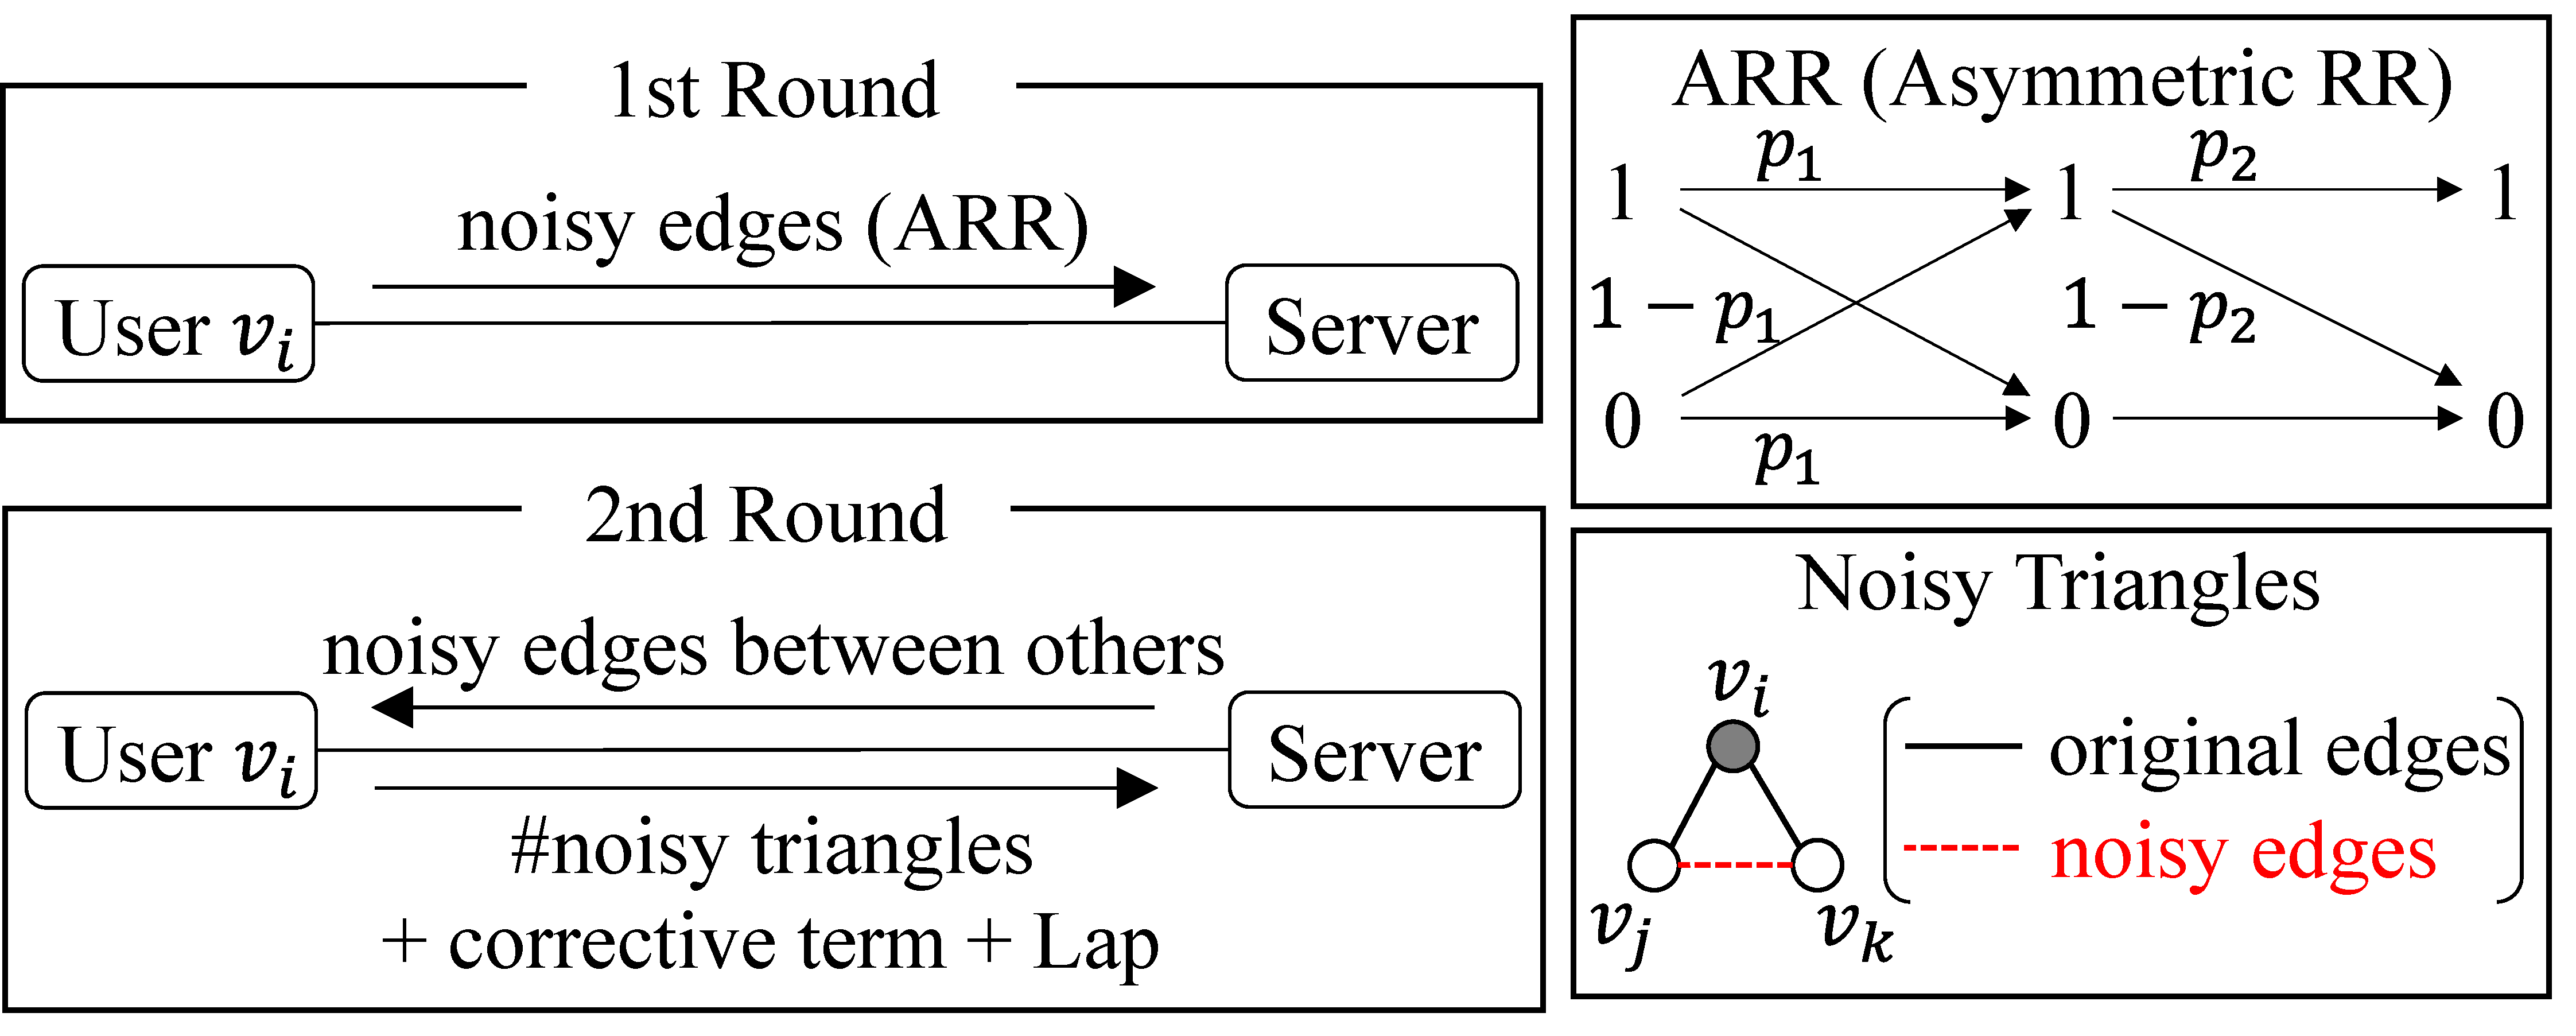
\includegraphics[width=0.99\linewidth]{fig/algorithm_overview.pdf}
  \vspace{-4mm}
  \caption{Overview of our communication-efficient triangle counting algorithms
  ($p_1 =\frac{e^{\epsilon}}{e^{\epsilon}+1}$,
  %$p_1 \in [\frac{1}{2},1]$,
  $p_2 \in [0,1]$).}
  %($\mu \in [0,1]$, $\rho = e^{-\epsilon_1}$).}
  %At the first round, each user obfuscates her edge by ARR ($\mu \in [0,1]$, $\rho \in e^{-\epsilon_1}$) to provide $\epsilon_1$-edge LDP.
  \label{chap2-fig:alg_overview}
\end{figure}

% \smallskip
% \noindent{\textbf{Our Two-Rounds Algorithms.}}~~
\smallskip
\noindent{\textbf{Algorithm Overview.}}~~Figure~\ref{chap2-fig:alg_overview} shows the overview of our proposed algorithms.
% all of which are run in two rounds.
% Below we explain the overview of our algorithms\footnote{For ease of explanation, we explain algorithms that use all elements in $\bmA$ in Section~\ref{chap2-sub:algorithms_overview}.
% In Section~\ref{chap2-sub:three_algorithms}, we propose algorithms that use only the lower triangular part of $\bmA$ to avoid the doubling issue, as described in Section~\ref{chap2-sub:LDP}.}.

At the first round, each user $v_i$ obfuscates
% $i-1$ bits for smaller user IDs in her neighbor list $\bma_i$ (i.e., lower triangular part of $\bmA$)
% each bit of her neighbor list $\bma_i$
% (for users with smaller user IDs)
bits for smaller user IDs in her neighbor list $\bma_i$
% (i.e., lower triangular part of $\bmA$)
by an LDP mechanism which we call the \textit{ARR (Asymmetric Randomized Response)} 
and sends the obfuscated bits to a server. 
% (note that we use only the lower triangular part of $\bmA$ to avoid the doubling issue, as described in Section~\ref{chap2-sub:LDP}).
The ARR is a combination of Warner's RR and edge sampling; i.e.,
we apply Warner's RR that outputs 1 or 0 as it is with probability
% $p_1\in[\frac{1}{2},1]$
$p_1$ ($=\frac{e^{\epsilon}}{e^{\epsilon}+1}$)
and then sample each 1 with probability $p_2\in[0,1]$.
%
% Given 1 (resp.~0) as input, the ARR outputs 1 with probability $\mu$ (resp.~$\mu\rho$), where $\mu \in [0,1]$, $\rho = e^{-\epsilon_1}$, and $\epsilon_1 \in \nnreals$.
% We can view this mechanism as a combination of Warner's RR~\cite{Warner_JASA65} and edge sampling; i.e., we apply Warner's RR that
% outputs 1 or 0 as it is with probability $p_1=\frac{e^{\epsilon_1}}{e^{\epsilon_1}+1}$
% and then sample each 1 with probability $p_2\in[0,1]$, where $\mu=p_1 p_2$.
% In fact, the ARR with $\mu = p_1$ (i.e., $p_2=1$) is equivalent to Warner's RR.
Unlike Warner's RR, the ARR is asymmetric in that the flip probability in the whole process is different
depending on the input value.
As with Warner's RR, the ARR provides edge LDP.
% Since Warner's RR provides
% $\epsilon_1$-
% edge LDP (as described in Section~\ref{chap2-sub:LDP}) and
% the sampling is a post-processing process (and
% DP is immune to post-processing~\cite{DP}, the ARR also provides
% $\epsilon_1$-
% edge LDP.
We can also significantly reduce the number of 1s (hence the communication cost) by setting
% the sampling probability
$p_2$ small.
% $\mu$ much smaller than $p_1$.
% Let $E' \subseteq V \times V$ be a set of noisy edges sent by users.

At the second round, the server calculates a message $M_i$ for user $v_i$ consisting of some or all noisy edges between others. 
We propose three strategies for calculating $M_i$. 
% and
% each user
User $v_i$ downloads $M_i$ from the server.
% a message $M_i$ from the server consisting of some or all
% of $E'$.
% noisy edges between others.
Then, since user $v_i$ knows her edges, $v_i$ can count \textit{noisy triangles} ($v_i$, $v_j$, $v_k$) such that $j<k<i$ and only one edge ($v_j$, $v_k$) is noisy, as shown in Figure~\ref{chap2-fig:alg_overview}. 
% $(v_i,v_j) \in E$, $(v_i,v_k) \in E$,
% $(v_j,v_k) \in E'$, and $j<k<i$;
% i.e., only one edge is noisy
The condition $j<k<i$ is imposed to use only the lower triangular part of $\bmA$, i.e., 
to avoid the doubling issue in Section~\ref{chap2-sub:LDP}. 
% Then $v_i$ adds some post-processing (to enable the server to obtain an unbiased estimate of $f_\triangle(G)$) and the Laplacian noise (to provide $\epsilon_2$-edge LDP for $\epsilon_2 \in \nnreals$) to the noisy triangle count, and sends it to a server.
User $v_i$ adds %some post-processing
a corrective term
%(to enable the server to obtain an unbiased estimate of $f_\triangle(G)$) 
and the Laplacian noise
% (to provide edge LDP)
to the noisy triangle count 
and sends it to a server.
The corrective term is added to enable the server to obtain an unbiased estimate of $f_\triangle(G)$. 
The Laplacian noise provides
% $\epsilon_2$-
edge LDP.
% , where $\epsilon_2 \in \nnreals$.
% From this,
Finally,
the server calculates an unbiased estimate of $f_\triangle(G)$
from the noisy data sent by users.
By composition (Proposition~\ref{chap2-prop:seq_comp_edge_LDP}),
% the compositionality of DP~\cite{DP},
our algorithms provide
% ($\epsilon_1 + \epsilon_2$)-
edge LDP in total.

\smallskip
\noindent{\textbf{Remark.}}~~Note that it is also possible for the server to calculate an unbiased estimate of $f_\triangle(G)$ at the first round.
However, this results in a
prohibitively
% very
large estimation error
% for a large graph
% for two reasons.
because
% First,
all edges sent by users are noisy; i.e., three edges are noisy in any triangle.
% all three edges are noisy in any triangle at the first round (whereas only one edge is noisy in our algorithms),
% Second, the noisy graph is dense, and consequently the time complexity of counting noisy triangles is $O(n^3)$. Thus, some approximation (such as edge sampling) is necessary to efficiently compute the estimate of $f_\triangle(G)$.
In contrast, only one edge is noisy in each noisy triangle at the second round because each user $v_i$ knows two original edges
% $(v_i,v_j) \in E$ and $(v_i,v_k) \in E$
connected to $v_i$.
Consequently, we can obtain an unbiased estimate with a much smaller variance.
See Appendix~\ref{chap2-sec:one-round} for a detailed comparison.
% In Appendix~\ref{chap2-sec:one-round}, we show that
% our two-rounds algorithms significantly outperform the existing one-round triangle algorithms.
% ~\cite{Imola_USENIX21,Ye_TKDE21}.
% (with sampling).
% the estimation error is significantly reduced by introducing an additional round.

% \subsection{Three Algorithms}
\subsection{Algorithms}
\label{chap2-sub:three_algorithms}

\smallskip
\noindent{\textbf{ARR.}}~~First, we formally define the ARR.
% We begin with a formal definition of the ARR.
% Below we describe our algorithms in detail.
The ARR has two parameters: $\epsilon \in \nnreals$ and $\mu \in [0,\frac{e^{\epsilon}}{e^{\epsilon} + 1}]$.
The parameter $\epsilon$ is the privacy budget, and $\mu$ controls the communication cost.

Let
% $\calR_{ARR}$
$ARR_{\epsilon,\mu}$ be the ARR with parameters $\epsilon$ and $\mu$. It takes $0/1$ as input and outputs $0/1$ with the following probability:
\begin{align}
    \Pr[ARR_{\epsilon,\mu}(1) = b] &= \begin{cases}\mu & (b=1) \\ 1-\mu & (b=0)\end{cases} \label{chap2-eq:ARR_1}\\
    \Pr[ARR_{\epsilon,\mu}(0) = b] &= \begin{cases}\mu\rho & (b=1) \\ 1-\mu \rho & (b=0), \end{cases} \label{chap2-eq:ARR_0}
\end{align}
where $\rho = e^{-\epsilon}$.
By Figure~\ref{chap2-fig:alg_overview},
we can view this randomizer as a combination of Warner's RR~\cite{Warner_JASA65}
% with $p_1=\frac{e^{\epsilon}}{e^{\epsilon}+1}$
and edge sampling, where $\mu=p_1 p_2$.
In fact, the ARR with $\mu = p_1 =\frac{e^{\epsilon}}{e^{\epsilon}+1}$ (i.e., $p_2=1$) is equivalent to Warner's RR.

Each user $v_i$ applies the ARR to bits for smaller user IDs in her neighbor list $\bma_i$; i.e., $\calR_i(\bma_i) = (ARR_{\epsilon,\mu}(a_{i,1}), \ldots, \allowbreak ARR_{\epsilon,\mu}(a_{i,i-1}))$.
% Note that we use only the lower triangular part of $\bmA$ to avoid the doubling issue described in Section~\ref{chap2-sub:LDP}.
Then $v_i$ sends $\calR_i(\bma_i)$ to the server.
% Applying Warner's RR to each bit of $\bma_i$ provides $\epsilon$-edge LDP (as described in Section~\ref{chap2-sub:LDP}).
Since applying Warner's RR to $\bma_i$ provides $\epsilon$-edge LDP (as described in Section~\ref{chap2-sub:LDP}) and the sampling is a post-processing process, applying the ARR to $\bma_i$ also provides $\epsilon$-edge LDP by the immunity to post-processing~\cite{DP}.

Let $E' \subseteq V \times V$ be a set of noisy edges sent by users.

\smallskip
\noindent{\textbf{Which Noisy Edges to Download?}}~~Now, the main question
tackled in this paper is: \textit{Which noisy edges should each user $v_i$
download at the second round?}
Note that
% user $v_i$ cannot leak her original edges to the server.
% For example,
user $v_i$
% cannot
is not allowed to
download only a set of noisy edges that form noisy triangles
(i.e., $\{(v_j,v_k) \in E' | (v_i,v_j) \in E, (v_i,v_k) \in E$\}),
% a set of noisy edges $\{(v_j,v_k) \in E' | (v_i,v_j) \in E, (v_i,v_k) \in E$\} (i.e., only noisy edges that form noisy triangles),
because it tells the server
% the fact that $v_j$ and $v_k$ are friends with $v_i$.
who are friends with $v_i$.
In other words, user $v_i$ cannot leak her original edges to the server when she
downloads noisy edges; the server must choose which part of $E'$ to include in
the message $M_i$ it sends her.

Thus, a natural solution would be to download \textit{all noisy edges between others}
% (except for the ones connected to $v_i$).
(with smaller user IDs); i.e.,
% \begin{align}
% M_i =\{(v_j, v_k) \in E' | j<k<i\}. \label{chap2-eq:M_i_I}
% \end{align}
$M_i =\{(v_j, v_k) \in E' | j<k<i\}$.
% as shown in Figure~\ref{chap2-fig:noisy_edge_DL}.
We denote our algorithm with this full download strategy by \AlgOne{}.
The (inefficient) two-rounds algorithm in~\cite{Imola_USENIX21} is a special case of \AlgOne{}
without sampling ($\mu = p_1$).
% when $\mu = p_1$ (i.e., when we
% use Warner's RR and
% do not sample edges).
In other words, \AlgOne{} is a generalization of the two-rounds algorithm in~\cite{Imola_USENIX21} using the ARR.
% $(v_j,v_k) \in E'$ such that $(v_i,v_j) \in E$, $(v_i,v_k) \in E$
% The expected download size in \AlgOne{} is $O(\mu n^2)$.

% Since users have already sent noisy edges at the first round, user $v_i$ can use noisy edges connected to $v_i$ when downloading noisy edges.
% For example,

In this paper,
we show that we can do much better
% we achieve much higher utility
than \AlgOne{}.
Specifically, we prove in Section~\ref{chap2-sub:algorithms_theoretical_analysis} that \AlgOne{} results in a high estimation error when the number of 4-cycles (cycles of length 4) in $G$ is large.
Intuitively, this can be explained as follows.
Suppose that $v_i$, $v_j$, $v_{i'}$, and $v_k$
($j<k<i$, $j<k<i'$)
form a 4-cycle. 
% $v_i-v_j-v_{i'}-v_k-v_i$.
% (denoted by $v_i$-$v_j$-$v_{i'}$-$v_k$).
% , as shown in the left panel of Figure~\ref{chap2-fig:four-cycle}.
There is no triangle in this graph.
However, if there is a noisy edge between $v_j$ and $v_k$, then two (incorrect) noisy triangles appear: ($v_i$, $v_j$, $v_k$) counted by $v_i$ and ($v_{i'}$, $v_j$, $v_k$) counted by $v_{i'}$.
More generally, let $E_{ijk}$ (resp.~$E_{i'jk}$) $\in \{0,1\}$ be a random variable that takes $1$ if ($v_i$, $v_j$, $v_k$) (resp.~($v_{i'}$, $v_j$, $v_k$)) forms a noisy triangle and $0$ otherwise.
Then, the covariance $\cov(E_{ijk},E_{i'jk})$ between $E_{ijk}$ and $E_{i'jk}$ is large because the presence/absence of a single noisy edge ($v_j$, $v_k$) affects the two noisy triangles.

To address this issue, we introduce a
% \textit{trick}
trick 
% trick, which we call the ``$4$-cycle trick'',
that makes the two noisy triangles \textit{less correlated with each other}.
We call this the \textit{4-cycle trick}.
% Since users have already sent noisy edges at the first round,
% user $v_i$ can use noisy edges connected to $v_i$ when downloading noisy edges.
Specifically,
% we propose two algorithms: \AlgTwo{} and \AlgThree{}.
we propose two algorithms in which
% user $v_i$ uses noisy edges connected to $v_i$ when downloading noisy edges.
the server uses noisy edges connected to $v_i$ when it calculates a message $M_i$ for $v_i$.
In the first algorithm,
% user $v_i$ downloads
the server selects
noisy edges $(v_j, v_k)$ such that
one noisy edge is connected from $v_k$ to $v_i$;
% there is a noisy edge between $v_i$ and $v_k$;
i.e.,
$M_i = \{(v_j, v_k) \in E' | (v_i, v_k) \in E', j<k<i\}$.
% \begin{align}
% M_i = \{(v_j, v_k) \in E' | (v_i, v_k) \in E', j<k<i\}. \label{chap2-eq:M_i_II}
% \end{align}
We call this algorithm \AlgTwo{}, as one noisy edge is connected to $v_i$.
In the second algorithm,
% user $v_i$ downloads
the server selects
noisy edges $(v_j, v_k)$ such that
two noisy edges are connected from these nodes to $v_i$; i.e.,
$M_i = \{(v_j, v_k) \in E' | (v_i, v_j) \in E', (v_i, v_k) \in E', j<k<i\}$.
% \begin{align}
% \hspace{-2mm} M_i \hspace{-0.5mm} = \hspace{-0.5mm}  \{(v_j, v_k) \in E' | (v_i, v_j) \in E', (v_i, v_k) \in E', j<k<i\}. \label{chap2-eq:M_i_III}
% \end{align}
We call this algorithm \AlgThree{}, as two noisy edges are connected to $v_i$.
Note that user $v_i$ does not leak her original edges to the server at the time of download in these algorithms, because
% $v_i$ uses only noisy edges the server has.
the server uses only noisy edges $E'$ sent by users to calculate $M_i$.

Figure~\ref{chap2-fig:noisy_edge_DL} shows our three algorithms.
% Let $\mu_F, \mu_O, \mu_T \in \nnreals$ be values of $\mu$ in the ARR used for \AlgOne{}, \AlgTwo{}, and \AlgThree{}, respectively.
% Then the
The download cost $\CostDL{}$ in (\ref{chap2-eq:cost_DL}) is
$O(\mu n^2 \log n)$, $O(\mu^2 n^2 \log n)$, and $O(\mu^3 n^2 \log n)$,
% $O(\mu_F n^2 \log n)$, $O(\mu_O^2 n^2 \log n)$, and $O(\mu_T^3 n^2 \log n)$,
respectively, when we regard $\epsilon$ as a constant.
In our experiments, we set
the parameter $\mu$ in the ARR so that
% $\mu$ in \AlgOne{}, $\mu^2$ in \AlgTwo{}, and $\mu^3$ in \AlgThree{} are equal
$\mu$ in \AlgOne{} is equal to $\mu^2$ in \AlgTwo{} and also equal to $\mu^3$ in \AlgThree{};
e.g., $\mu=10^{-6}$, $10^{-3}$, and $10^{-2}$ in \AlgOne{}, \AlgTwo{}, and \AlgThree{}, respectively.
% $\mu_F$, $\mu_O$, and $\mu_T$ to $\mu_F = \mu_O^2 = \mu_T^3$ (e.g., $\mu_F=10^{-6}$, $\mu_O=10^{-3}$, $\mu_T=10^{-2}$)
% so that
% the expected download size
Then
the download cost
is the same between the three algorithms.

\begin{figure}[t]
  \centering
  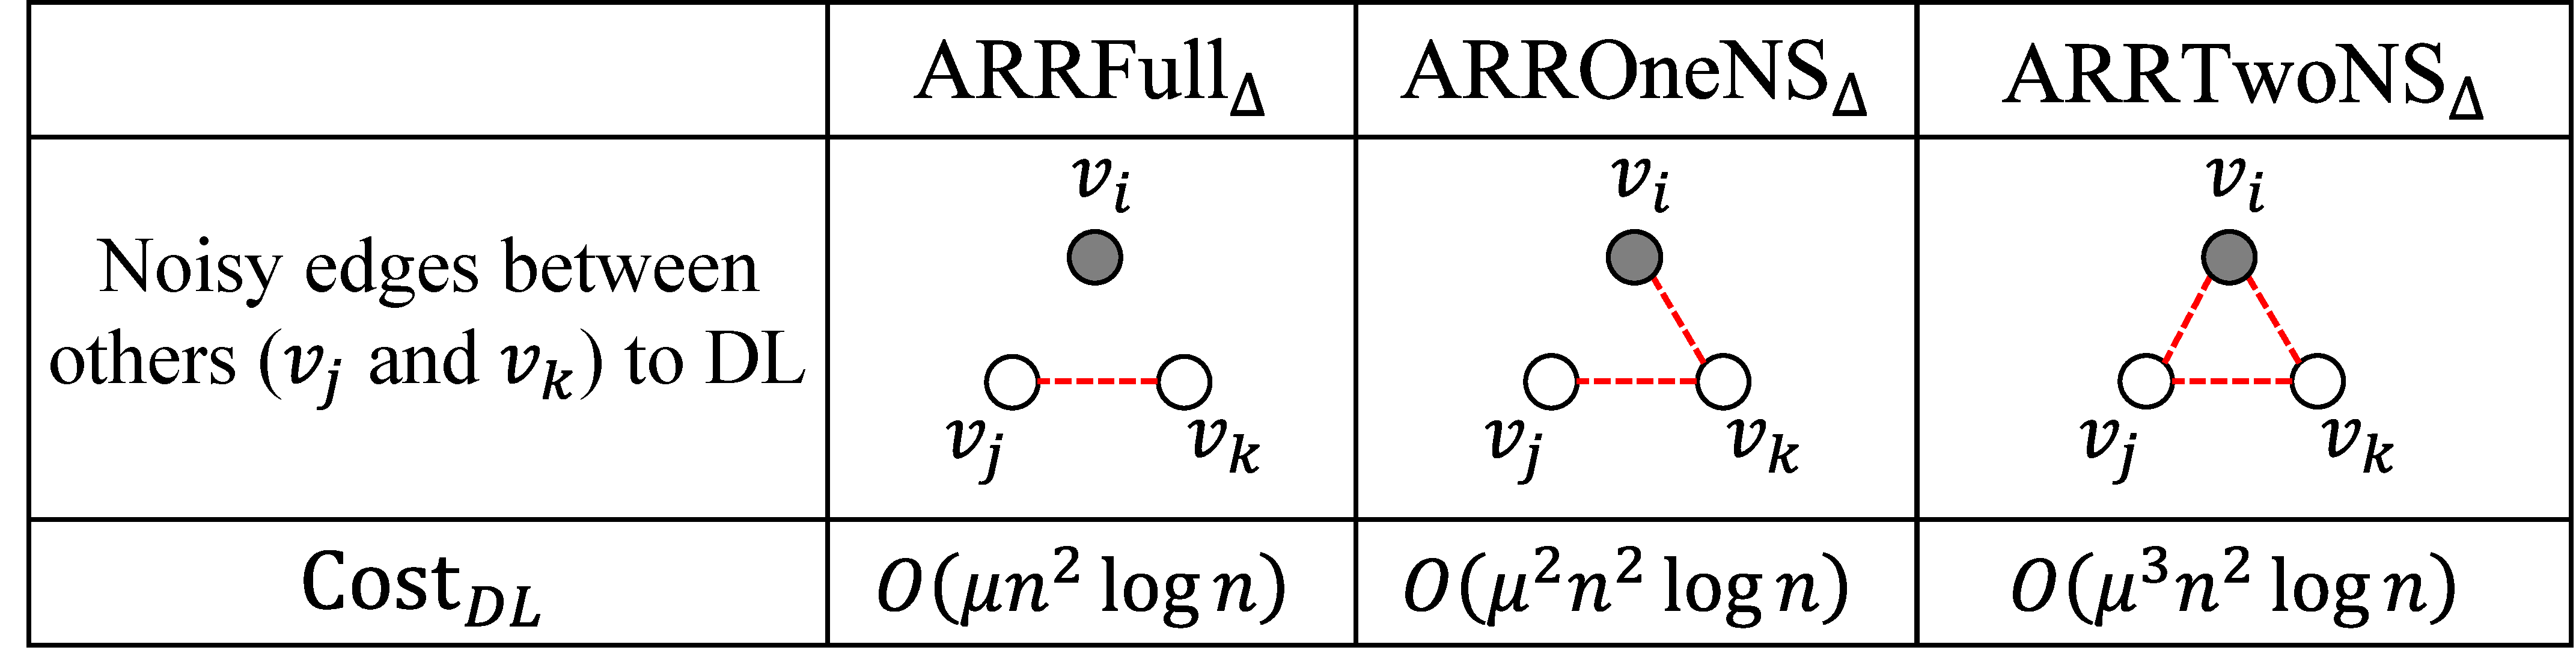
\includegraphics[width=0.99\linewidth]{fig/three_algorithms.pdf}
  \vspace{-4mm}
  \caption{Noisy edges to download
  % and expected download size
  in our three algorithms.}
  %$\mu_F$, $\mu_O$, and $\mu_T$ are values of $\mu$ in the ARR used for \AlgOne{}, \AlgTwo{}, and \AlgThree{}, respectively.}
  \label{chap2-fig:noisy_edge_DL}
% \end{figure}
\vspace{4mm}
% \begin{figure}[t]
  \centering
  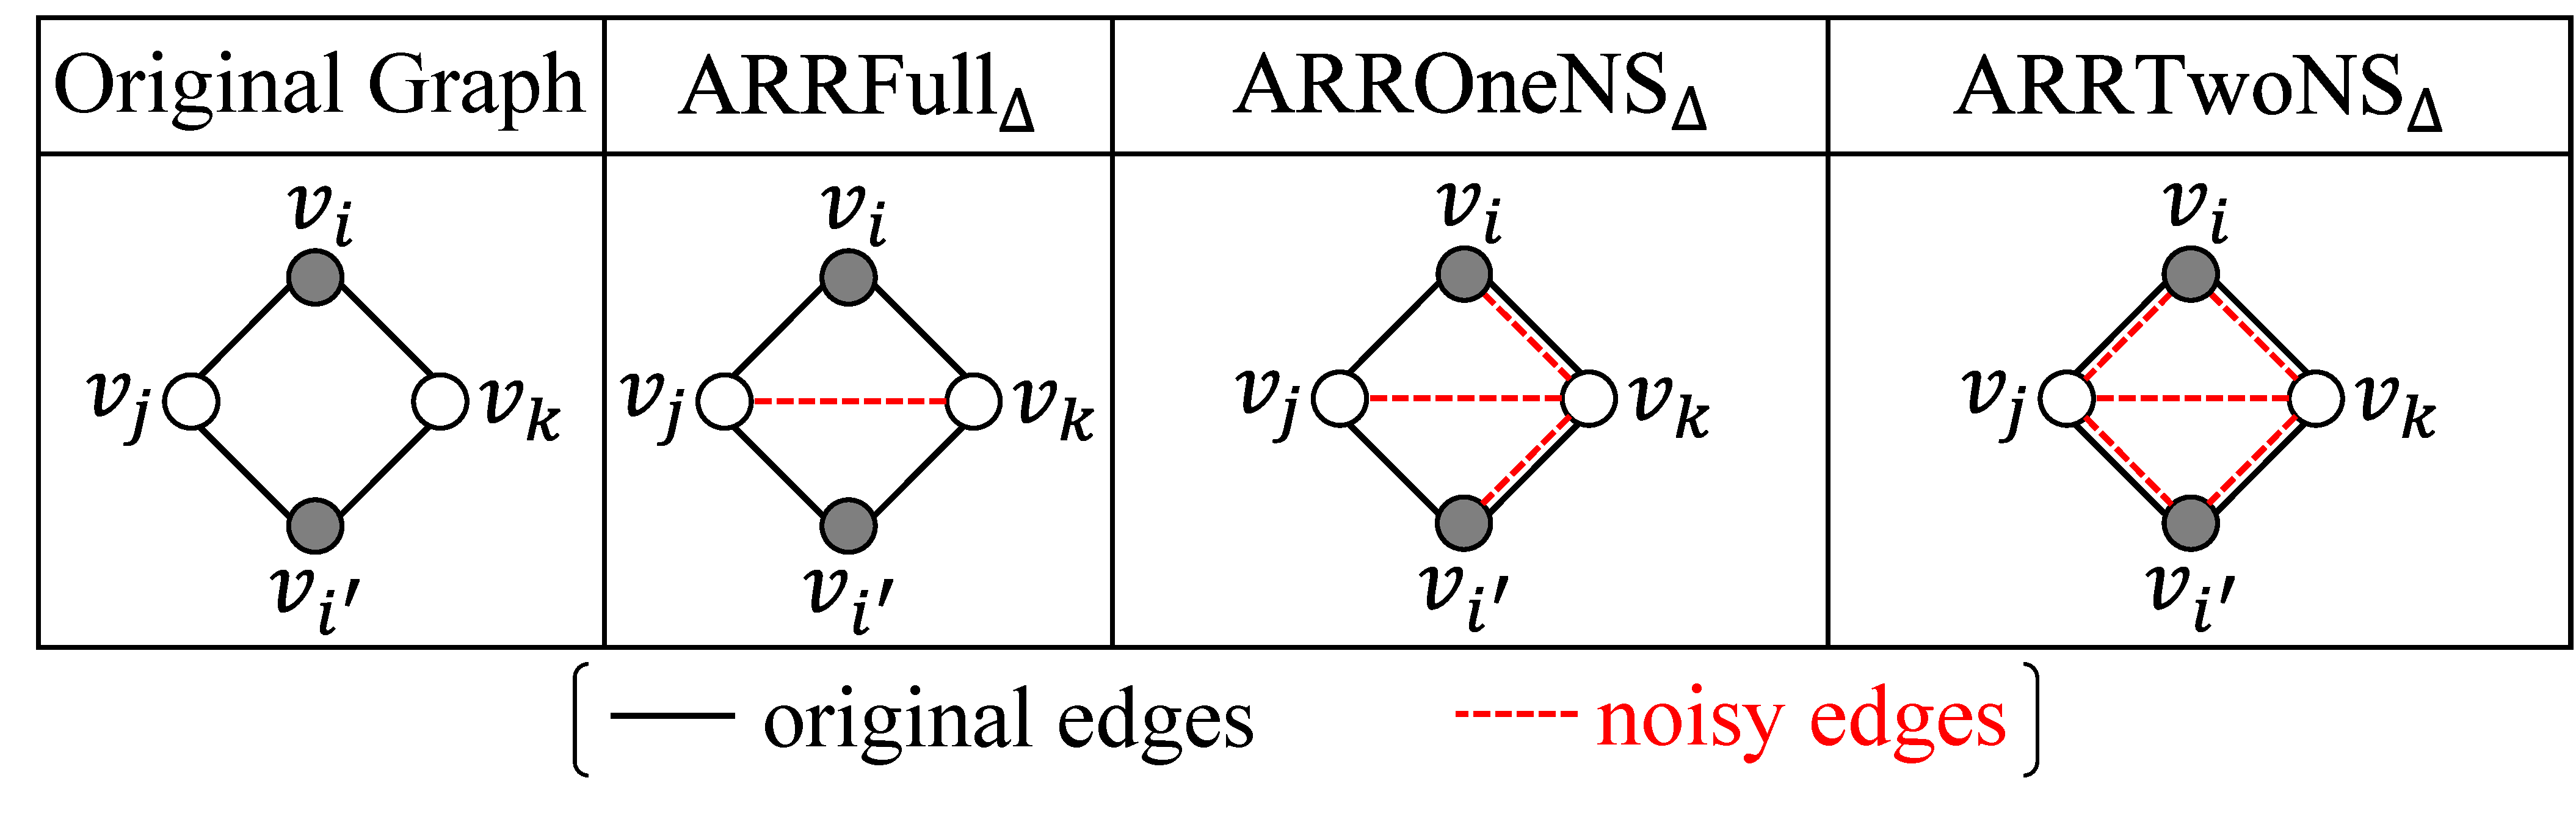
\includegraphics[width=0.95\linewidth]{fig/four_cycle.pdf}
  \vspace{-4mm}
  \caption{4-cycle trick.
  % 4-cycle issue.
  \AlgOne{} counts two (incorrect) noisy triangles when one noisy edge appears.
  \AlgTwo{} and \AlgThree{} avoid this by increasing independent noise.}
  \label{chap2-fig:four-cycle}
\end{figure}

% Figure\ref{chap2-fig:four-cycle} shows why and how \AlgTwo{} and \AlgThree{} address the 4-cycle issue.
Figure~\ref{chap2-fig:four-cycle} shows our $4$-cycle trick.
\AlgOne{} counts two (incorrect) noisy triangles when a noisy edge ($v_j$, $v_k$) appears.
% there is a noisy edge ($v_j$, $v_k$).
In contrast,
% the two noisy triangles are counted
\AlgTwo{} (resp.~\AlgThree{}) counts both the two noisy triangles
% this bad event happens
only when three (resp.~five) independent noisy edges appear,
% in \AlgTwo{} (resp.~\AlgThree{}),
as shown in Figure~\ref{chap2-fig:four-cycle}.
% Since these noisy edges are independent,
Thus, this bad event happens with a much smaller probability.
For example,
% when $\mu_F=10^{-6}$, $\mu_O=10^{-3}$, and $\mu_T=10^{-2}$,
% \AlgOne{}, \AlgTwo{}, and \AlgThree{} count both the two noisy triangles with probability $10^{-6}$, $10^{-9}$, and $10^{-10}$, respectively.
\AlgOne{} ($\mu=10^{-6}$),
\AlgTwo{} ($\mu=10^{-3}$), and
\AlgThree{} ($\mu=10^{-2}$)
count both the two noisy triangles with probability $10^{-6}$, $10^{-9}$, and $10^{-10}$, respectively.
The covariance $\cov(E_{ijk},E_{i'jk})$ of \AlgTwo{} and \AlgThree{} is also much smaller than that of \AlgOne{}.
% \AlgTwo{} and \AlgThree{} also achieve much smaller covariance $\cov(E_{ijk},E_{i'jk})$ than \AlgOne{}.


In our experiments, we show that \AlgTwo{} and \AlgThree{} significantly outperforms \AlgOne{}
% in two real graph datasets with a large number of 4-cycles.
for a large-scale graph or dense graph, in both of which
% when
the number of 4-cycles in $G$ 
% can be very 
is 
large.
% \ji{Are there other scenarios where the performance is better?}
% \commentT{I think the number of 4-cycles can be large when a graph is (i) large or (ii) dense (in particular, (i) is important). I clarified this.}

\smallskip
\noindent{\textbf{\AlgTwo{} vs. \AlgThree{}.}}~~One
% The number of independent noisy edges in a 4-cycle is three and five in \AlgTwo{} and \AlgThree{}, respectively, as shown in Figure\ref{chap2-fig:four-cycle}.
% Thus
might expect that \AlgThree{} outperforms \AlgTwo{} because \AlgThree{} addresses the 4-cycle issue more aggressively; i.e.,
% \AlgThree{} has the largest number of independent noisy edges in a 4-cycle,
the number of independent noisy edges in a 4-cycle is larger in \AlgThree{},
as shown in Figure \ref{chap2-fig:four-cycle}.
However,
% \AlgThree{} suffers from a large global sensitivity of the Laplacian noise at the second round.
\AlgTwo{} can reduce the global sensitivity of the Laplacian noise
at the second round
more effectively than \AlgThree{}, as explained in Section~\ref{chap2-sec:double_clip}.
% in detail.
Consequently, \AlgTwo{}, which is the most tricky algorithm, achieves the smallest estimation error in our experiments.
See Sections~\ref{chap2-sec:double_clip} and \ref{chap2-sec:experiments} for details of the global sensitivity and experiments, respectively.

\smallskip
\noindent{\textbf{Three Algorithms.}}~~Below we explain the details of our three algorithms.
For ease of explanation, we assume that the maximum degree $d_{max}$ is public in Section~\ref{chap2-sub:three_algorithms}\footnote{For example, $d_{max}$ is public in Facebook: $d_{max} = 5000$~\cite{Facebook_Limit}.
If the server does not have prior knowledge about $d_{max}$, she can privately estimate $d_{max}$ and use graph projection to guarantee that each user's degree never exceeds the private estimate of $d_{max}$~\cite{Imola_USENIX21}.
In any case, the assumption in Section~\ref{chap2-sub:three_algorithms} does not undermine our algorithms, because our entire algorithms with double clipping in Section~\ref{chap2-sec:double_clip} does \textit{not} assume that $d_{max}$ is public.}.
Note, however, that
% we propose a technique to significantly reduce the global sensitivity
our double clipping (which is proposed to significantly reduce the global sensitivity) in Section~\ref{chap2-sec:double_clip} does \textit{not} assume that $d_{max}$ is public.
Consequently, our entire algorithms 
% (i.e., \AlgOne, \AlgTwo, \AlgThree with double clipping)
% three triangle counting algorithms (\AlgOne, \AlgTwo, \AlgThree) with our double clipping
do \textit{not} require the assumption that $d_{max}$ is public.

\setlength{\algomargin}{5mm}
\begin{algorithm}[t]
  \SetAlgoLined
  \KwData{Graph $G \in \calG$ represented as neighbor lists $\bma_1, \ldots, \bma_n
    \in \{0,1\}^n$, privacy budgets
  $\epsilon_1,\epsilon_2 \in \nnreals$, $d_{max} \in \nnints$,
  $\mu \in [0,\frac{e^{\epsilon_1}}{e^{\epsilon_1} + 1}]$.
  %$\mu^*$.
  }
  \KwResult{Private estimate $\hf_\triangle(G)$ of $f_\triangle(G)$.}
%   $p_1 \leftarrow \frac{1}{e^{\epsilon_1}}$\;
  [s] $\rho \leftarrow e^{-\epsilon_1}$\;
  [$v_i$, s] $\mu^* \leftarrow \mu$, $\mu^2$, and $\mu^3$ in F, O, and T, respectively\;
  \tcc{First round.}
  \For{$i=1$ \KwTo $n$}{
    [$v_i$] $\bmr_i \leftarrow (ARR_{\epsilon_1,\mu}(a_{i,1}), \ldots,
    ARR_{\epsilon_1,\mu}(a_{i,i-1}))$\;
    [$v_i$] Upload $\bmr_i = (r_{i,1}, \ldots, r_{i,i-1})$ to the server\;
  }
%   $E' = \{(v_i, v_j) : i > j, r_{i,j} = 1\} \cup \{(v_j, v_i) : i > j, r_{i,j} =
%   1\}$\;
  [s] $E' = \{(v_j, v_k) :r_{k,j} = 1, j < k\}$\;
  \tcc{Second round.}
  \For{$i=1$ \KwTo $n$}{
    [s] Compute
    $M_i$ by (\ref{chap2-eq:M_i_I}), (\ref{chap2-eq:M_i_II}), and (\ref{chap2-eq:M_i_III}) in F, O, and T, respectively\;
    %$M_i = \{(v_j,v_k) \in E': j < k < i\}$\;
    %$M_i = \{(v_j,v_k) \in E': (v_i,v_k) \in E', j < k < i\}$\;
    %$M_i = \{(v_j,v_k) \in E': (v_i,v_k), (v_j,v_k) \in E', j < k < i\}$\;
    [$v_i$] Download $M_i$ from the server\;
    [$v_i$] $t_i \leftarrow |\{(v_i,v_j,v_k) :
    a_{i,j} = a_{i,k} = 1, (v_j,v_k) \in M_i, j<k<i \}|$\;
    [$v_i$] $s_i \leftarrow |\{(v_i,v_j,v_k) :
    a_{i,j} = a_{i,k} = 1, j<k<i\}|$\;
    [$v_i$] $w_i \leftarrow t_i - \mu^* \rho s_i$\;
    [$v_i$] $\hw_i \leftarrow w_i + \Lap(\frac{d_{max}}{\epsilon_2})$\;
    [$v_i$] Upload $\hw_i$ to the server\;
  }
  [s] $\hf_\triangle(G) \leftarrow \frac{1}{\mu^*(1-\rho)}\sum_{i=1}^n \hw_i$\;
  \KwRet{$\hf_\triangle(G)$}
  \caption{Our three algorithms.
  ``F'', ``O'', ``T'' are shorthands for
  %$\mu^*=\mu_F$, $\mu_O^2$, and $\mu_T^3$ in
  \AlgOne{}, \AlgTwo{}, and \AlgThree{}, respectively.
  [$v_i$] and [s] represent that the process is run by $v_i$ and the server, respectively.
  }\label{chap2-alg:unify}
\end{algorithm}

% As explained above,
Recall that the server calculates a message $M_i$ for $v_i$ as:
\begin{align}
\hspace{-1mm} M_i \hspace{-0.5mm} &= \hspace{-0.5mm} \{(v_j, v_k) \in E' | j<k<i\} \label{chap2-eq:M_i_I}\\
\hspace{-1mm} M_i \hspace{-0.5mm} &= \hspace{-0.5mm} \{(v_j, v_k) \in E' | (v_i, v_k) \in E', j<k<i\} \label{chap2-eq:M_i_II}\\
\hspace{-1mm} M_i \hspace{-0.5mm} &= \hspace{-0.5mm}  \{(v_j, v_k) \in E' | (v_i, v_j) \in E', (v_i, v_k) \in E', j<k<i\} \label{chap2-eq:M_i_III}
\end{align}
in \AlgOne{}, \AlgTwo{}, \AlgThree{}, respectively.

%Using these equations,
% our three algorithms can be unified in Algorithm~\ref{chap2-alg:unify}.
Algorithm~\ref{chap2-alg:unify} shows our three algorithms.
These algorithms are processed differently in lines 2 and 9; ``F'', ``O'', ``T'' are shorthands for \AlgOne{}, \AlgTwo{}, and \AlgThree{}, respectively.
% It uses two rounds of private computation, and
% in both rounds each user $v_i$ applies a local randomizer to her neighbor list $\bma_i$.
The privacy budgets for the first and second
rounds are $\epsilon_1, \epsilon_2 \in \nnreals$, respectively.

The first round appears in lines 3-7 of Algorithm~\ref{chap2-alg:unify}.
In this round, each user applies
$ARR_{\epsilon_1, \mu}$
% the ARR
defined by (\ref{chap2-eq:ARR_1}) and (\ref{chap2-eq:ARR_0}) to bits $a_{i,1}, \ldots, a_{i,i-1}$ for smaller user IDs in her neighbor list $\bma_i$, i.e., lower triangular part of $\bmA$.
% explained in the beginning of
% Section~\ref{chap2-sub:three_algorithms}.
Let $\bmr_i = (r_{i,1}, \ldots, r_{i,i-1}) \in \{0,1\}^{i-1}$ be the obfuscated bits of $v_i$.
User $v_i$ uploads $\bmr_i$ to the server.
Then the server combines the noisy edges together, forming $E' = \{(v_j, v_k) : r_{k,j} = 1, j < k\}$.

The second round appears in lines 8-17 of Algorithm~\ref{chap2-alg:unify}.
In this round, the server computes a message $M_i$
by (\ref{chap2-eq:M_i_I}), (\ref{chap2-eq:M_i_II}), or (\ref{chap2-eq:M_i_III}),
% depending on the algorithm,
and user $v_i$ downloads it.
% As explained above, \AlgOne{}, \AlgTwo{}, and \AlgThree{} computes $M_i$ by (\ref{chap2-eq:M_i_I}), (\ref{chap2-eq:M_i_II}), and  (\ref{chap2-eq:M_i_III}), respectively.
Then user $v_i$ calculates the number $t_i \in \nnints$ of noisy triangles ($v_i$, $v_j$, $v_k$) such that
% $j<k<i$ and
only one edge ($v_j$, $v_k$) is noisy, as shown in Figure~\ref{chap2-fig:alg_overview}.
% involving two edges in user $v_i$'s neighbor list and one noisy edge in $E'$ (as shown in Figure~\ref{chap2-fig:alg_overview}).
% We also emphasize that the condition $j<k<i$ is imposed to use only the lower triangular part of $\bmA$.
% (and avoid the doubling issue).
User $v_i$ also calculate a corrective term $s_i \in \nnints$.
The corrective term $s_i$ is the number of
possible triangles involving $v_i$ 
% that can be formed from edges in $v_i$'s neighbor list,
and is computed to obtain an unbiased estimate of $f_\triangle(G)$.
% unbias the triangle count.
User $v_i$ calculates $w_i = t_i - \mu^* \rho s_i$, where $\rho = e^{-\epsilon_1}$ and
% $\mu^* = \mu_F$, $\mu_O^2$, and $\mu_T^3$
$\mu^* = \mu$, $\mu^2$, and $\mu^3$
in ``F'', ``O'', and ``T'', respectively.
% \AlgOne{}, \AlgTwo{}, and \AlgThree{}, respectively.
Then $v_i$ adds the Laplacian noise $\Lap(\frac{d_{max}}{\epsilon_2})$ to $w_i$ to provide $\epsilon_2$-edge LDP and sends the noisy value $\hw_i$ ($= w_i + \Lap(\frac{d_{max}}{\epsilon_2})$) to the server. 
Note that adding one edge increases both $t_i$ and $s_i$ 
% results in the increase of the triangle count 
by at most $d_{max}$. 
Thus, the global sensitivity of $w_i$ is at most $d_{max}$. 
Finally, the server calculates an estimate of $f_\triangle(G)$ as: $\hf_\triangle(G) = \frac{1}{\mu^*(1-\rho)}\sum_{i=1}^n \hw_i$.
As we prove later, $\hf_\triangle(G)$ is an unbiased estimate of $f_\triangle(G)$.

% \smallskip
% \noindent{\textbf{\AlgOne.}}

% Our first algorithm, \AlgOne, appears in Algorithm~\ref{chap2-alg:one}. It uses two
% rounds of private computation, and in both rounds each user applies a local
% randomizer to his data.
% The privacy budgets for the two
% rounds are $\epsilon_1, \epsilon_2$.

% The first round appears in Lines 3-4 of Algorithm~\ref{chap2-alg:one}. This round
% collects the noisy edges from the users.
% The noisy edges are produced
% using the asymmetric randomized response mechanism, which we denote
% $ARR_{\epsilon, \mu}$. Recall that a bit $a_{i,j}$ of $\bma_i$ takes value $1$
% if and only if user $v_i$ includes user $v_j$ in his neighbor list. ARR is
% defined by $\Pr[ARR_{\epsilon, \mu}(1) = 1] = \mu$ and $\Pr[ARR_{\epsilon,
% \mu}(0) = 1] = \mu p_1$ where $p_1 = e^{-\epsilon_1}$. User $v_i$ uploads
% $\bmr_i$, the vector of ARR mechanisms applied to $a_{i,j}$ for $j < i$. This
% means that user $v_i$ ignores users with a bigger index than $i$. By doing so,
% for every possible undirected edge $(v_i, v_j)$, exactly one of $v_i, v_j$ will
% upload the
% edge using ARR. This prevents releasing the edge twice, and allows us to prove
% that our mechanism satisfies relationship DP without the doubling factor in
% $\epsilon$ (see Proposition~\ref{chap2-prop:edge_LDP_entire_edge_LDP}).
% Given the collection of ARR queries to the users, the server concludes the first
% round by combining the noisy edges together and unordering them, forming $E'$.

% The second round appears in Lines 8-13 of Algorithm~\ref{chap2-alg:one}.
% In this round, each user $v_i$ computes an unbiased estimator $w_i$ for
% the number of triangles involving $v_i$ for which the maximum index of the
% triangle is $i$. It is easy to see that the sum of the $w_i$ estimates the total
% number of triangles. The user does this by
% downloading the message $M = E'$ from the server
% and computing a noisy triangle count $t_i$ and a corrective term $s_i$. The count
% $t_i$ is the number of triangles involving two edges in user $v_i$'s neighbor
% list and one noisy edge in $E'$. The corrective term $s_i$ is the number of
% possible triangles that can be formed from edges in user $v_i$'s neighbor list,
% and is computed to unbias the triangle count. We emphasize that user $v_i$
% only considers the part of his neighbor list involving users of a lower index
% than $i$ for all calculations, including this. The unbiased estimator is
% given by $w_i = t_i - \mu_F p_1 s_i$---because it depends on the private data
% $\bma_i$, the user adds Laplacian noise of width $\frac{d_{max}}{\epsilon_2}$ to
% $w_i$ that the computation may satisfy $\epsilon_2$ edge LDP. He then uploads
% the noisy value $\hw_i$, and the server computes the final triangle estimate.

% \begin{algorithm}
%   \SetAlgoLined
%   \KwData{Graph $G$ represented as neighbor lists $\bma_1, \ldots, \bma_n
%     \in \{0,1\}^n$, two privacy budgets
%   $\epsilon_1,\epsilon_2 > 0$, $d_{max} \in \nnints$, sampling parameter
%   $\mu_F$.}
%   \KwResult{Private estimate of $f_\triangle(G)$.}
%   $p_1 \leftarrow \frac{1}{e^{\epsilon_1}}$\;
%   \tcc{First round.}
%   \For{$i=1$ \KwTo $n$}{
%     $\bmr_i \leftarrow (ARR_{\epsilon_1,\mu_F}(a_{i,1}), \ldots,
%     ARR_{\epsilon_1,\mu_F}(a_{i,i-1}))$\;
%     Upload $\bmr_i$ to server\;
%   }
%   $E' = \{(v_j, v_i) : i > j, r_{i,j} = 1\}$\;
%   \tcc{Second round.}
%   \For{$i=1$ \KwTo $n$}{
%     Server lets $M_i = E'$.
%     Download $M_i$ from server\;
%     $t_i \leftarrow |\{(v_i,v_j,v_k) :
%     j<k<i, a_{i,j} = a_{i,k} = 1, (k,j) \in M \}|$\;
%     $s_i \leftarrow |\{(v_i,v_j,v_k) :
%     j<k<i, a_{i,j} = a_{i,k} = 1\}|$\;
%     $w_i \leftarrow t_i - \mu_F p_1 s_i$\;
%     $\hw_i \leftarrow w_i + \Lap(\frac{d_{max}}{\epsilon_2})$\;
%     Upload $\hw_i$ to server\;
%   }
%   \KwRet{$\frac{1}{\mu_F(1-p_1)}\sum_{i=1}^n \hw_i$}
%   \caption{\AlgOne}\label{chap2-alg:one}
% \end{algorithm}

% \smallskip
% \noindent{\textbf{\AlgTwo.}}

% Our second Algorithm, \AlgTwo, appears in Algorithm~\ref{chap2-alg:two}. Like
% \AlgOne, it uses two rounds with budgets $\epsilon_1$ and $\epsilon_2$.
% The first round is identical to \AlgOne, and for brevity, Algorithm~\ref{chap2-alg:two} does not
% include a description of the first round.
% Recall that the goal of the second round is for each user $v_i$ to compute an estimate of the
% number of triangles in which $i$ is the maximum index, which is the variable
% $\hw_i$.
% The difference between \AlgOne and
% \AlgTwo is that in the second round of \AlgTwo (Lines 2-8), a user only downloads a
% subset of edges in
% $E'$: $v_i$ downloads those edges $(v_j, v_k) \in E'$ such that $j < k < i$ and
% $v_i \text{\----} v_k \text{\----} v_j$ are connected in $E'$. The server is
% able to compute these edges since they only depend on the first round release,
% and we denote it with $M_i$. User $v_i$ then computes his estimate $w_i = t_i -
% \mu_O^2 p_1 s_i$, where $t_i$ is and $s_i$ are the same quantities as in
% \AlgOne. The final estimator $w_i = t_i - \mu_O^2
% p_1 s_i$ is an unbiased estimate of the number of triangles for which $i$ is the
% maximum index. User $v_i$ uploads $\hw_i$, given by $w_i$ plus Laplace noise, in
% order to share $w_i$ privately.

% Downloading only some of $E'$, depending on the noisy first round, actually
% produces a noisier estimator $\hw_i$ than \AlgOne. However, the communication
% cost of \AlgTwo is less, precisely because a subset of $E'$ is downloaded. It
% is straightforward to prove that in expectation, user $v_i$ downloads $\mu_F
% n^2$ edges in \AlgOne and $\mu_O^2 n^2$ edges in \AlgTwo. Thus, the two
% algorithms have comparable communication when $\mu_F = \mu_O^2$, meaning that
% $\mu_F \ll \mu_O$. Thus, \AlgOne is forced to sample edges at a much smaller
% ratio than \AlgTwo in the first round, producing a much noisier value of $E'$.
% At these two different sampling ratios, the estimator $\hw_i$ in \AlgTwo is not
% necessarily worse than the same estimator in \AlgOne

% \begin{algorithm}
%   \SetAlgoLined
%   \KwData{Graph $G$ represented as neighbor lists $\bma_1, \ldots, \bma_n
%     \in \{0,1\}^n$, two privacy budgets
%   $\epsilon_1,\epsilon_2 > 0$, $d_{max} \in \nnints$, sampling parameter
%   $\mu_O$.}
%   \KwResult{Private estimate of $f_\triangle(G)$.}
%   \tcc{Second round.}
%   \For{$i=1$ \KwTo $n$}{
%     Server computes $M_i = \{(j,k) : j < k < i, (k,i), (j,k) \in E'\}$\;
%     Download $M_i$ from server\;
%     $t_i \leftarrow |\{(v_i,v_j,v_k) :
%     j<k<i, a_{i,j} = a_{i,k} = 1, (j,k) \in M_i\}|$\;
%     $s_i \leftarrow |\{(v_i,v_j,v_k) :
%     j<k<i, a_{i,j} = a_{i,k} = 1\}|$\;
%     $w_i \leftarrow t_i - \mu_O^2 p_1 s_i$\;
%     $\hw_i \leftarrow w_i + \Lap(\frac{d_{max}}{\epsilon_2})$\;
%     Upload $\hw_i$ to server\;
%   }
%   \KwRet{$\frac{1}{\mu_O^2(1-p_1)}\sum_{i=1}^n \hw_i$}
%   \caption{\AlgTwo, second round only (first round is identical to \AlgOne with
%   sampling parameter $\mu_O$).}\label{chap2-alg:two}
% \end{algorithm}

% \smallskip
% \noindent{\textbf{\AlgThree.}}~~TBD
% \colorB{\begin{itemize}
%     \item Algorithm of \AlgThree (only the 2nd round).
% \end{itemize}}

% \begin{algorithm}
%   \SetAlgoLined
%   \KwData{Graph $G$ represented as neighbor lists $\bma_1, \ldots, \bma_n
%     \in \{0,1\}^n$, two privacy budgets
%   $\epsilon_1,\epsilon_2 > 0$, $d_{max} \in \nnints$, sampling parameter
%   $\mu_T$.}
%   \KwResult{Private estimate of $f_\triangle(G)$.}
%   \tcc{Second round.}
%   \For{$i=1$ \KwTo $n$}{
%     Server computes $M_i = \{(j,k) : j < k < i, (k,i), (j,k), (j,i) \in E'\}$\;
%     Download $M_i$ from server\;
%     $t_i \leftarrow |\{(v_i,v_j,v_k) :
%     j<k<i, a_{i,j} = a_{i,k} = 1, (j,k) \in M_i \}|$\;
%     $s_i \leftarrow |\{(v_i,v_j,v_k) :
%     j<k<i, a_{i,j} = a_{i,k} = 1\}|$\;
%     $w_i \leftarrow t_i - \mu_T^3 p_1 s_i$\;
%     $\hw_i \leftarrow w_i + \Lap(\frac{d_{max}}{\epsilon_2})$\;
%     Upload $\hw_i$ to server\;
%   }
%   \KwRet{$\frac{1}{\mu_T^3(1-p_1)}\sum_{i=1}^n \hw_i$}
%   \caption{\AlgThree, second round only (first round is identical to \AlgOne
%   with sampling parameter $\mu_T$).}\label{chap2-alg:three}
% \end{algorithm}

% \smallskip
% \noindent{\textbf{Summary.}}~~TBD
% \colorB{\begin{itemize}
%     \item One algorithm table unifying all three algorithms (e.g., $\mu^* = \mu_F$, $\mu_o^2$, $\mu_T^3$ in \AlgOne, \AlgTwo, and \AlgThree, respectively).
% \end{itemize}}

\subsection{Theoretical Analysis}
\label{chap2-sub:algorithms_theoretical_analysis}
We now introduce the theoretical guarantees on
% theoretically analyze
the privacy, communication, and
utility of 
our algorithms. 
% \AlgOne{}, \AlgTwo{}, and \AlgThree{}.
% All the proofs appear in Appendix~\ref{chap2-sec:proof_algorithms}.
% The first round of the
% algorithms is all the same: Each user applies a randomizer $\calR_i^1(\bma_i)$
% to his neighbor list which releases the ARR of his neighbors. Then, the server
% computes $M_i$ in a different way depending on the algorithm.
% Let $M_i^F, M_i^O,
% M_i^T$ be the message $M_i$ used in \AlgOne{}, \AlgTwo{}, and \AlgThree{}, respectively.
% Formulas for these values appear in
% equations~\eqref{chap2-eq:M_i_I},~\eqref{chap2-eq:M_i_II}, and~\eqref{chap2-eq:M_i_III},
% respectively.
% For fixed $M_i$ and $\mu^*$, the second round of the algorithms is
% also the same, and we denote it with $\calR_i^{2}(M_i, \mu^*)(\bma_i)$, where $\mu^* =
% \mu, \mu^2, \mu^3$ depending on \AlgOne{}, \AlgTwo{}, or \AlgThree{}. Notice
% that the final triangle estimate $\hf_\triangle(G)$ is given by a post-processing of
% $\{\calR_i^2(M_i, \mu^*)(\bma_i) : 1 \leq i \leq n\}$.

% \paragraph{Privacy}
\smallskip
\noindent{\textbf{Privacy.}}~~We first show the privacy guarantees:
% The privacy guarantee of our three algorithms comes from proving that
% $\calR_i^1(\bma_i)$ and $\calR_i^2(M_i, \mu^*)(\bma_i)$ satisfies $\epsilon$-edge DP for any choice of $M_i, \mu^*$,
% they satisfy $\epsilon_1$ and $\epsilon_2$-edge LDP at the first and second round, respectively,
% $\epsilon$-edge DP for any choice of $M_i, \mu^*$,
% and then using sequential composition (Proposition~\ref{chap2-prop:seq_comp_edge_LDP}):
% and post-processing:
\begin{theorem}\label{chap2-thm:privacy_algorithms}
  % Let $\mu, d_{max}$ be fixed.
  For $i \in [n]$,
  let
%   $\calR_i^1, \calR_i^2(M_i, \mu^*)$
  $\calR_i^1, \calR_i^2(M_i)$
  be the randomizers used by user $v_i$ in
  rounds $1$ and $2$ of Algorithm~\ref{chap2-alg:unify}. % where $M_i = M_i^F, M_i^O$, or $M_i^T$.
  Let
%   $\calR_i(\bma_i) = (\calR_i^1(\bma_i), \calR_i^2(M_i, \mu^*)(\bma_i))$
  $\calR_i(\bma_i) = (\calR_i^1(\bma_i), \calR_i^2(M_i)(\bma_i))$
  be the composition of the two randomizers. Then,
  $\calR_i$
%   $\calR_i$ satisfies $(\epsilon_1 + \epsilon_2)$-edge LDP for $i \in [n]$, and $(\calR_1,
%   \ldots, \calR_n)$ satisfies $(\epsilon_1 + \epsilon_2)$-relationship DP.
%   Thus, by post-processing, the output of Algorithm~\ref{chap2-alg:unify}
  satisfies
  $(\epsilon_1+\epsilon_2)$-edge LDP and
  $(\calR_1,
  \ldots, \calR_n)$ satisfies  $(\epsilon_1+\epsilon_2)$-relationship DP.
\end{theorem}

% A full proof of this claim appears in Appendix~\ref{chap2-sec:proof_algorithms}.
% The algorithms satisfy both $(\epsilon_1+\epsilon_2)$-edge LDP and $(\epsilon_1+\epsilon_2)$-relationship DP
Note that the doubling issue in Section~\ref{chap2-sub:LDP} does not occur, 
because we use only the lower triangular part of $\bmA$. 
% (i.e., avoid the doubling issue in Section~\ref{chap2-sub:LDP}).
% each user ignores edges in her neighbor list to users with smaller index than his own.
% Thus, each edge affects the output of at most one randomizer in
% each round. This allows us to prove a tighter bound on the relationship DP
% parameter than that given by Proposition~\ref{chap2-prop:edge_LDP_entire_edge_LDP}.
By the immunity to post-processing, the estimate  $\hf_\triangle(G)$
% in Algorithm~\ref{chap2-alg:unify}
also satisfies $(\epsilon_1+\epsilon_2)$-edge LDP and $(\epsilon_1+\epsilon_2)$-relationship DP.

% \paragraph{Communication}
\smallskip
\noindent{\textbf{Communication.}}~~Recall that we evaluate the algorithms based on their download cost~\eqref{chap2-eq:cost_DL} and upload cost~\eqref{chap2-eq:cost_UL}.

\textit{Download Cost:} The download cost is the number of bits required
to download $M_i$.
% Each user can represent $M_i$
$M_i$ can be represented
as
% pairs of edges, which
a list of edges between others, and each edge
can be
identified with two indices (user IDs), i.e., $2 \log n$ bits.
% Thus, the total communication is $2 (\log n)\E[|M_i|]$.
% The number of edges in $M_i$ depends on \AlgOne{}, \AlgTwo{}, and \AlgThree{}.
There are $\frac{(n-1)(n-2)}{2} \approx \frac{n^2}{2}$ edges between others.
% Given 1 (resp.~0) as input, $ARR_{\epsilon_1,\mu}$ outputs 1 with probability $\mu$ (resp.~$\mu e^{- \epsilon_1}$).
$ARR_{\epsilon_1,\mu}$ outputs 1 with probability at most $\mu$. 
% When $d_{max} \ll n$, most input values are 0.
In addition, each noisy triangle must have $1$, $2$, and $3$ noisy edges in \AlgOne{}, \AlgTwo{}, and \AlgThree{}, respectively, as shown in Figure~\ref{chap2-fig:noisy_edge_DL}.

Thus, 
% when $d_{max} \ll n$, 
the download cost in Algorithm~\ref{chap2-alg:unify} 
% for each algorithm 
can be written as:
% ($F$, $O$, and $T$ are shorthands for \AlgOne{}, \AlgTwo{}, and \AlgThree{}, respectively):
% Notice that any element $(v_j, v_k)$ is included independently in $E'$ with
% probability at most $\mu$. Any element $(v_j, v_k)$ appears in $M_i^F$ (resp. $M_i^O$, $M_i^T$)
% if and only if $1$ (resp. $2,3$) other elements appears in $E'$. Thus, the
% probability an element appears in $M_i^F$ (resp. $M_i^O, M_i^T$) is at most
% $\mu$ (resp. $\mu^2, \mu^3$).
% Hence, $\E[|M_i^F|] \leq \mu \binom{n}{2}$, $\E[|M_i^O|] \leq \mu^2 \binom{n}{2}$,
% and $\E[|M_i^F|] \leq \mu^3 \binom{n}{2}$. In summary, we have (where $F,O,T$ is a
% shorthand for \AlgOne{}, \AlgTwo{}, and \AlgThree{}),
\begin{align}
   Cost_{DL} &\leq \mu^* n^2 \log n,  \label{chap2-eq:CostDL_F}
%   Cost_{DL}(F) &\leq \mu n^2 \log n,  \label{chap2-eq:CostDL_F}\\
%   Cost_{DL}(O) &\leq \mu^2 n^2 \log n \label{chap2-eq:CostDL_O}\\
%   Cost_{DL}(T) &\leq \mu^3 n^2 \log n. \label{chap2-eq:CostDL_T}
%   Cost_{DL}(F) &\leq \mu n^2 \log n \label{chap2-eq:CostDL_F}\\
%   Cost_{DL}(O) &\leq \mu^2 n^2 \log n \label{chap2-eq:CostDL_O}\\
%   Cost_{DL}(T) &\leq \mu^3 n^2 \log n. \label{chap2-eq:CostDL_T}
%   Cost_{DL}(F) &\approx \mu e^{-\epsilon_1} n^2 \log n \label{chap2-eq:CostDL_F}\\
%   Cost_{DL}(O) &\approx \mu^2 e^{-\epsilon_1} n^2 \log n \nonumber\\
%   Cost_{DL}(T) &\approx \mu^3 e^{-\epsilon_1} n^2 \log n. \nonumber
%   Cost_{DL}(F) &= \max_{i=1}^n 2(\log n) \E[|M_i^F|] \leq \mu n^2 \log n \\
%   Cost_{DL}(O) &= \max_{i=1}^n 2(\log n) \E[|M_i^O|] \leq \mu^2 n^2 \log n \\
%   Cost_{DL}(T) &= \max_{i=1}^n 2(\log n) \E[|M_i^T|] \leq \mu^3 n^2 \log n
\end{align}
where $\mu^* = \mu$, $\mu^2$, and $\mu^3$ in \AlgOne{}, \AlgTwo{}, and \AlgThree{}, respectively. 
In (\ref{chap2-eq:CostDL_F}), 
% (\ref{chap2-eq:CostDL_O}), and (\ref{chap2-eq:CostDL_T}), 
we upper-bounded $\CostDL{}$ by using the fact that $ARR_{\epsilon_1,\mu}$ outputs 1 with probability at most $\mu$. 
However, when $d_{max} \ll n$, 
$ARR_{\epsilon_1,\mu}$ outputs 1 with probability $\mu e^{- \epsilon_1}$ in most cases. 
In that case, we can roughly approximate $\CostDL{}$ by replacing $\mu$ with $\mu e^{- \epsilon_1}$ in (\ref{chap2-eq:CostDL_F}). 
% , (\ref{chap2-eq:CostDL_O}), and (\ref{chap2-eq:CostDL_T}). 
% In our experiments, we also confirmed that this approximation is accurate up to three significant digits.

\textit{Upload Cost:}
% For each of the three algorithms,
The upload cost comes
from the number of bits required to upload $\calR_i^1(\bma_i)$ and
% $\calR_i^2(M_i, \mu^*)(\bma_i)$.
$\calR_i^2(M_i)(\bma_i)$.
Uploading $\calR_i^1(\bma_i)$ involves uploading
$\bmr_i$ (line 5), which is a list of up to $n$ noisy neighbors. By sending just
the indices (user IDs) of the $1$s in $\bmr_i$, each user sends $\|\bmr_i\|_1 \log n$ bits,
where $\|\bmr_i\|_1$ is the number of 1s in $\bmr_i$.
% (note that $\log n$ bits are required to express each index).
When we use $ARR_{\epsilon_1,\mu}$,
% defined by (\ref{chap2-eq:ARR_1}) and (\ref{chap2-eq:ARR_0}),
we have $\E[\|\bmr_i\|_1] \leq \mu n$.
% since the probability of any bit of $\bmr_i$ is
% at most $\mu$.
% Moreover, $\E[\|\bmr_i\|_1] \approx \mu e^{-\epsilon_1} n$ when $d_{max} \ll n$.
% for a sparse graph where each bit in the original graph $G$ is $0$ in most cases.
% 
% For any choice of $M_i, \mu^*$,
Uploading
% $\calR_i^2(M_i, \mu^*)$
$\calR_i^2(M_i)$
involves uploading a single real number $\hw_i$ (line 15), which is negligibly small (e.g., 64 bits when we use a double-precision floating-point).
% While it is
% theoretically possible for $\hw_i$ to
% have arbitrarily large magnitude due to the Laplace noise, $\hw_i$ can be
% clipped and rounded so that it can be sent accurately with $O(\log n)$ bits. We
% do not provide a theoretical analysis of how to do this because the upload cost of
% the first round is much higher.

Thus,
% when $d_{max} \ll n$, 
the upload cost in Algorithm~\ref{chap2-alg:unify} can be written as:
% approximated as:
% for each of the three algorithms, we have
%
\begin{align}
%   Cost_{UL} = \max_{i=1}^n \E[\|\bmr_i\|_1]\log n + \E[bits(\hw_i)] = O(\mu n \log n).
%   Cost_{UL} \approx \mu e^{- \epsilon_1} n \log n.
  Cost_{UL} \leq \mu n \log n.
% \]
\label{chap2-eq:CostUL_proposal}
\end{align}
% where $\mu$ is $\mu_F$, $\mu_O$, and $\mu_T$ in \AlgOne{}, \AlgTwo{}, and \AlgThree{}, respectively.
Clearly, 
% the upload cost 
$\CostUL{}$ 
is much smaller than 
% the download cost 
$\CostDL{}$ 
for large $n$.

% \paragraph{Utility}
\smallskip
\noindent{\textbf{Utility.}}~~Analyzing the expected $l_2$ loss $l_2^2(f_\triangle(G), \hf_\triangle(G))$ of the algorithms involves first proving that
the estimator $\hf_\triangle$ is unbiased
% (i.e., for any graph $G$, $\E[\hf_\triangle(G)] = f_\triangle(G)$)
and then
% . Then, we
% control
analyzing
the
variance $\V[\hf_\triangle(G)]$ to obtain an upper-bound on
$l_2^2(f_\triangle(G), \hf_\triangle(G))$.
This is given in the following:

\begin{theorem}\label{chap2-thm:l2loss_algorithms}
  %Let $G, \mu, \epsilon$ be fixed.
  Let $G \in \calG$, $\epsilon_1, \epsilon_2 \in \nnreals$, and
  $\mu \in [0,\frac{e^{\epsilon_1}}{e^{\epsilon_1} + 1}]$.
%   $\mu_F, \mu_O, \mu_T \in [0,\frac{e^{\epsilon}}{e^{\epsilon_1} + 1}]$.
  %Let $G$, $\mu_F$, $\mu_O$, and $\mu_T$ be fixed.
  Let $\hf_\triangle^F(G), \hf_\triangle^O(G)$,
  and $\hf_\triangle^T(G)$ be
  the
  % estimators returned
  estimates output
  respectively by \AlgOne{}, \AlgTwo{}, and \AlgThree{} in Algorithm~\ref{chap2-alg:unify}.
  %, respectively.
  Then, $\E[\hf_\triangle^F(G)] = \E[\hf_\triangle^O(G)] = \E[\hf_\triangle^T(G)] = f_\triangle(G)$ (i.e., estimates are unbiased) and
   %Furthermore,
   %when no Laplace noise is added (i.e. $\epsilon_2 = \infty$),
   %we have:
   \begin{align*}
      l_2^2(f_\triangle(G), \hf_\triangle^F(G)) &\leq \textstyle{\frac{2C_4(G)+S_2(G)}{\mu(1-e^{\epsilon_1})^2} + \frac{2nd_{max}^2}{\mu^2(1-e^{\epsilon_1})^2\epsilon_2^2}} \\
      l_2^2(f_\triangle(G), \hf_\triangle^O(G)) &\leq \textstyle{\frac{\mu(2 C_4(G) + 6S_3(G)) + S_2(G)}{\mu^2(1-e^{\epsilon_1})^2} \hspace{-0.5mm}+\hspace{-0.5mm} \frac{2nd_{max}^2}{\mu^4(1-e^{\epsilon_1})^2\epsilon_2^2}}\\
      l_2^2(f_\triangle(G), \hf_\triangle^T(G)) &\leq \textstyle{\frac{\mu^2(2 C_4(G) + 6S_3(G)) + S_2(G)}{\mu^3(1-e^{\epsilon_1})^2} \hspace{-0.5mm}+\hspace{-0.5mm} \frac{2nd_{max}^2}{\mu^6(1-e^{\epsilon_1})^2\epsilon_2^2},}
   \end{align*}
   where $C_4(G)$ is the number of $4$-cycles in $G$
   %$P_3(G)$ is the number of $3$-paths in $G$,
   and $S_k(G)$ is the number of $k$-stars in $G$. %(see Figure~\ref{chap2-fig:subgraphs} in Appendix~\ref{chap2-sec:notations_subgraphs} for their shapes).
   %For a general $\epsilon_2$, the above quantities increase by an additive factor of
   %$2n \left(\frac{d_{max}}{\mu^*(1-e^{\epsilon_1})\epsilon_2}\right)^2$.
\end{theorem}
For each of the three upper-bounds in Theorem~\ref{chap2-thm:l2loss_algorithms}, the first and second terms are the estimation errors caused by empirical estimation and the Laplacian noise, respectively.
We also note that
% $C_4(G) = P_3(G) = S_3(G) = O(n d_{max}^3)$
$C_4(G) = S_3(G) = O(n d_{max}^3)$
and $S_2(G) = O(n d_{max}^2)$.
% when we regard $\epsilon_1$ and $\epsilon_2$ as constants.
Thus, for small
% $\mu_F$ ($=\mu_O^2 = \mu_T^3$),
$\mu$,
the $l_2$ loss of empirical estimation can be expressed as $O(n d_{max}^3)$, $O(n d_{max}^2)$, and $O(n d_{max}^2)$ in \AlgOne{}, \AlgTwo{}, \AlgThree{}, respectively
% (when we regard $\epsilon_1$ as a constant),
% (as the factors of $S_3(G)$ and $P_3(G)$
% diminish for small $\mu$).
(as the factors of $C_4(G)$ and $S_3(G)$
diminish for small $\mu$).
% can be removed by $\mu$.
% The large $l_2$ loss of \AlgOne{} is caused by the number $C_4$ of $4$-cycles that is written as $O(n d_{max}^3)$.

This highlights our $4$-cycle trick.
The large $l_2$ loss of \AlgOne{} is caused by the number $C_4(G) = O(n d_{max}^3)$ of $4$-cycles.
\AlgTwo{} and \AlgThree{} addresses this issue by increasing independent noise, as shown in Figure~\ref{chap2-fig:four-cycle}.
% The theorem highlights the $4$-cycle issue of \AlgOne{}, because its utility guarantee depends on the number of $4$-cycles in $G$. While the number of $4$-cycles is strictly less than the number of $3$-paths, the other algorithms benefit from being able to set $\mu$ higher, and thus sample less.

% However,
% % all of our three algorithms still suffer from a very large estimation error. due to a large amount of the Laplacian noise.
% all of the upper-bounds in Theorem~\ref{chap2-thm:l2loss_algorithms} are still very large.
% % due to a large amount of the Laplacian noise (as shown in our experiments).
% % In particular,
% This is because
% the Laplacian noise is very large especially for small $\epsilon_2$ or
% % $\mu_F$ ($=\mu_O^2 = \mu_T^3$),
% $\mu$,
% as shown in Theorem~\ref{chap2-thm:l2loss_algorithms}.
% % In Section~\ref{chap2-sec:double_clip}, we introduce a double clipping technique to significantly reduce the amount of Laplacian noise.
% In
% % Section~\ref{chap2-sec:double_clip},
% the next section,
% we introduce \textit{double clipping} to significantly reduce the amount of Laplacian noise.

% our three algorithms

% \begin{figure}
%   \begin{tabular}{|l|l|l|l|}
%     \hline
%     & \AlgOne & \AlgTwo & \AlgThree \\ \hline
%     Privacy & $\epsilon_1 + \epsilon_2$ & $\epsilon_1 + \epsilon_2$ &
%     $\epsilon_1 + \epsilon_2$ \\ \hline
%     Utility & $\frac{1}{\mu_F(1-e^{-\epsilon_1})}O\left( \square(G) + \wedge(G)
%     + \frac{2nd_{max}^2}{\mu_F \epsilon_2^2}\right)$ & 0
%     & 0 \\ \hline
%     $\text{Cost}_{DL}$ & $\mu_F n^3 \log n$ & $\mu_O^2 n^3 \log n$ & $\mu_T^3
%     n^3 \log n$ \\ \hline
%     $\text{Cost}_{UL}$ & $\mu_Fn \log n$ & $\mu_O n \log n$ & $\mu_T n \log n$ \\ \hline
%   \end{tabular}
% \end{figure}

\section{Double Clipping}
\label{chap2-sec:double_clip}

% However, 
% all of our three algorithms still suffer from a very large estimation error. due to a large amount of the Laplacian noise. 
In Section~\ref{chap2-sec:algorithms}, 
% \ref{chap2-sub:algorithms_theoretical_analysis}, 
we showed that the estimation error caused by empirical estimation (i.e., the first term in Theorem~\ref{chap2-thm:l2loss_algorithms}) is significantly reduced by the $4$-cycle trick. 
However, 
% all of the upper-bounds in 
the estimation error is 
% caused by the Laplacian noise (i.e., the second term)  
% Theorem~\ref{chap2-thm:l2loss_algorithms} are 
still very large in our algorithms presented in Section~\ref{chap2-sec:algorithms}, as shown in our experiments. 
% due to a large amount of the Laplacian noise (as shown in our experiments). 
% In particular, 
This is because 
the estimation error by the Laplacian noise (i.e., the second term in Theorem~\ref{chap2-thm:l2loss_algorithms}) 
% the Laplacian noise 
is very large, especially for small $\epsilon_2$ or 
% $\mu_F$ ($=\mu_O^2 = \mu_T^3$), 
$\mu$. 
% as shown in Theorem~\ref{chap2-thm:l2loss_algorithms}. 
% In Section~\ref{chap2-sec:double_clip}, we introduce a double clipping technique to significantly reduce the amount of Laplacian noise.
This error term is tight and unavoidable as long as we use $d_{max}$ as a global sensitivity, which suggests that we need a better global sensitivity analysis.
% In 
% Section~\ref{chap2-sec:double_clip}, 
% the next section, 
% we introduce \textit{double clipping} to significantly reduce the amount of Laplacian noise.
% 
% Our three algorithms in Section~\ref{chap2-sec:algorithms} suffer from a large amount of the Laplacian noise. 
% due to the large global sensitivity. 
% To address this issue, 
% Thus, we propose a double clipping technique, which significantly reduces the global sensitivity of the Laplacian noise. 
To significantly reduce the global sensitivity, we propose a novel \textit{double clipping} technique. 
% Therefore, we propose a double clipping technique, which significantly reduces the global sensitivity of the Laplacian noise. 

We describe the overview and details of our double clipping in Sections~\ref{chap2-sub:clip_overview} and \ref{chap2-sub:algorithms}, respectively. 
Then we perform theoretical analysis in Section~\ref{chap2-sub:clip_theoretical_analysis}.

\subsection{Overview}
\label{chap2-sub:clip_overview}

% \smallskip
\noindent{\textbf{Motivation.}}~~Figure~\ref{chap2-fig:reduce_noisy_triangles} shows noisy triangles involving edge $(v_i,v_j)$ counted by user $v_i$ in our three algorithms. 
Our algorithms in Section~\ref{chap2-sec:algorithms} 
% (and the two-rounds algorithm in \cite{Imola_USENIX21}) 
use the fact that the number of such noisy triangles (hence the global sensitivity) is upper-bounded by the maximum degree $d_{max}$ because 
%user $v_i$'s degree is at most $d_{max}$). 
adding one edge increases the triangle count by at most $d_{max}$. 
Unfortunately, this upper-bound is too large, as shown in our experiments. 
% Although this is correct, we 

% Our basic idea is that we can 
In this paper, we 
significantly reduce this upper-bound by using the parameter $\mu$ in the ARR and user $v_i$'s degree $d_i \in \nnints$ for users with smaller IDs. 
For example, 
% we can expect that 
the number of noisy triangles involving $(v_i,v_j)$ in \AlgOne is 
expected to be around 
$\mu d_i$ 
% ($\mu \ll 1$, $d_i < d_{max}$) 
% with high probability (larger than $0.5$) 
because one noisy edge is included in each noisy triangle (as shown in Figure~\ref{chap2-fig:reduce_noisy_triangles}) and all noisy edges are independent. 
$\mu d_i$ is very small, especially when we set $\mu \ll 1$ to reduce the communication cost.  
% Similarly, the expected number of noisy triangles involving $(v_i,v_j)$ in \AlgTwo is $\mu_O^2 d_i$ because two independent noisy edges are in each noisy triangle (as in Figure~\ref{chap2-fig:reduce_noisy_triangles}).

However, we cannot directly use $\mu d_i$ as an upper-bound of the global sensitivity in \AlgOne for two reasons. 
First, $\mu d_i$ leaks the exact value of user $v_i$'s degree $d_i$ 
and 
% , hence 
violates edge LDP. 
% friendship information of $v_i$ (e.g., as an extreme example, $d_i=0$ reveals the fact that $v_i$ has no friends). 
Second, the number of noisy triangles involving $(v_i,v_j)$ exceeds $\mu d_i$ with high probability (about $0.5$). 
Thus, the noisy triangle count cannot be upper-bounded by $\mu d_i$. 

\begin{figure}[t]
  \centering
  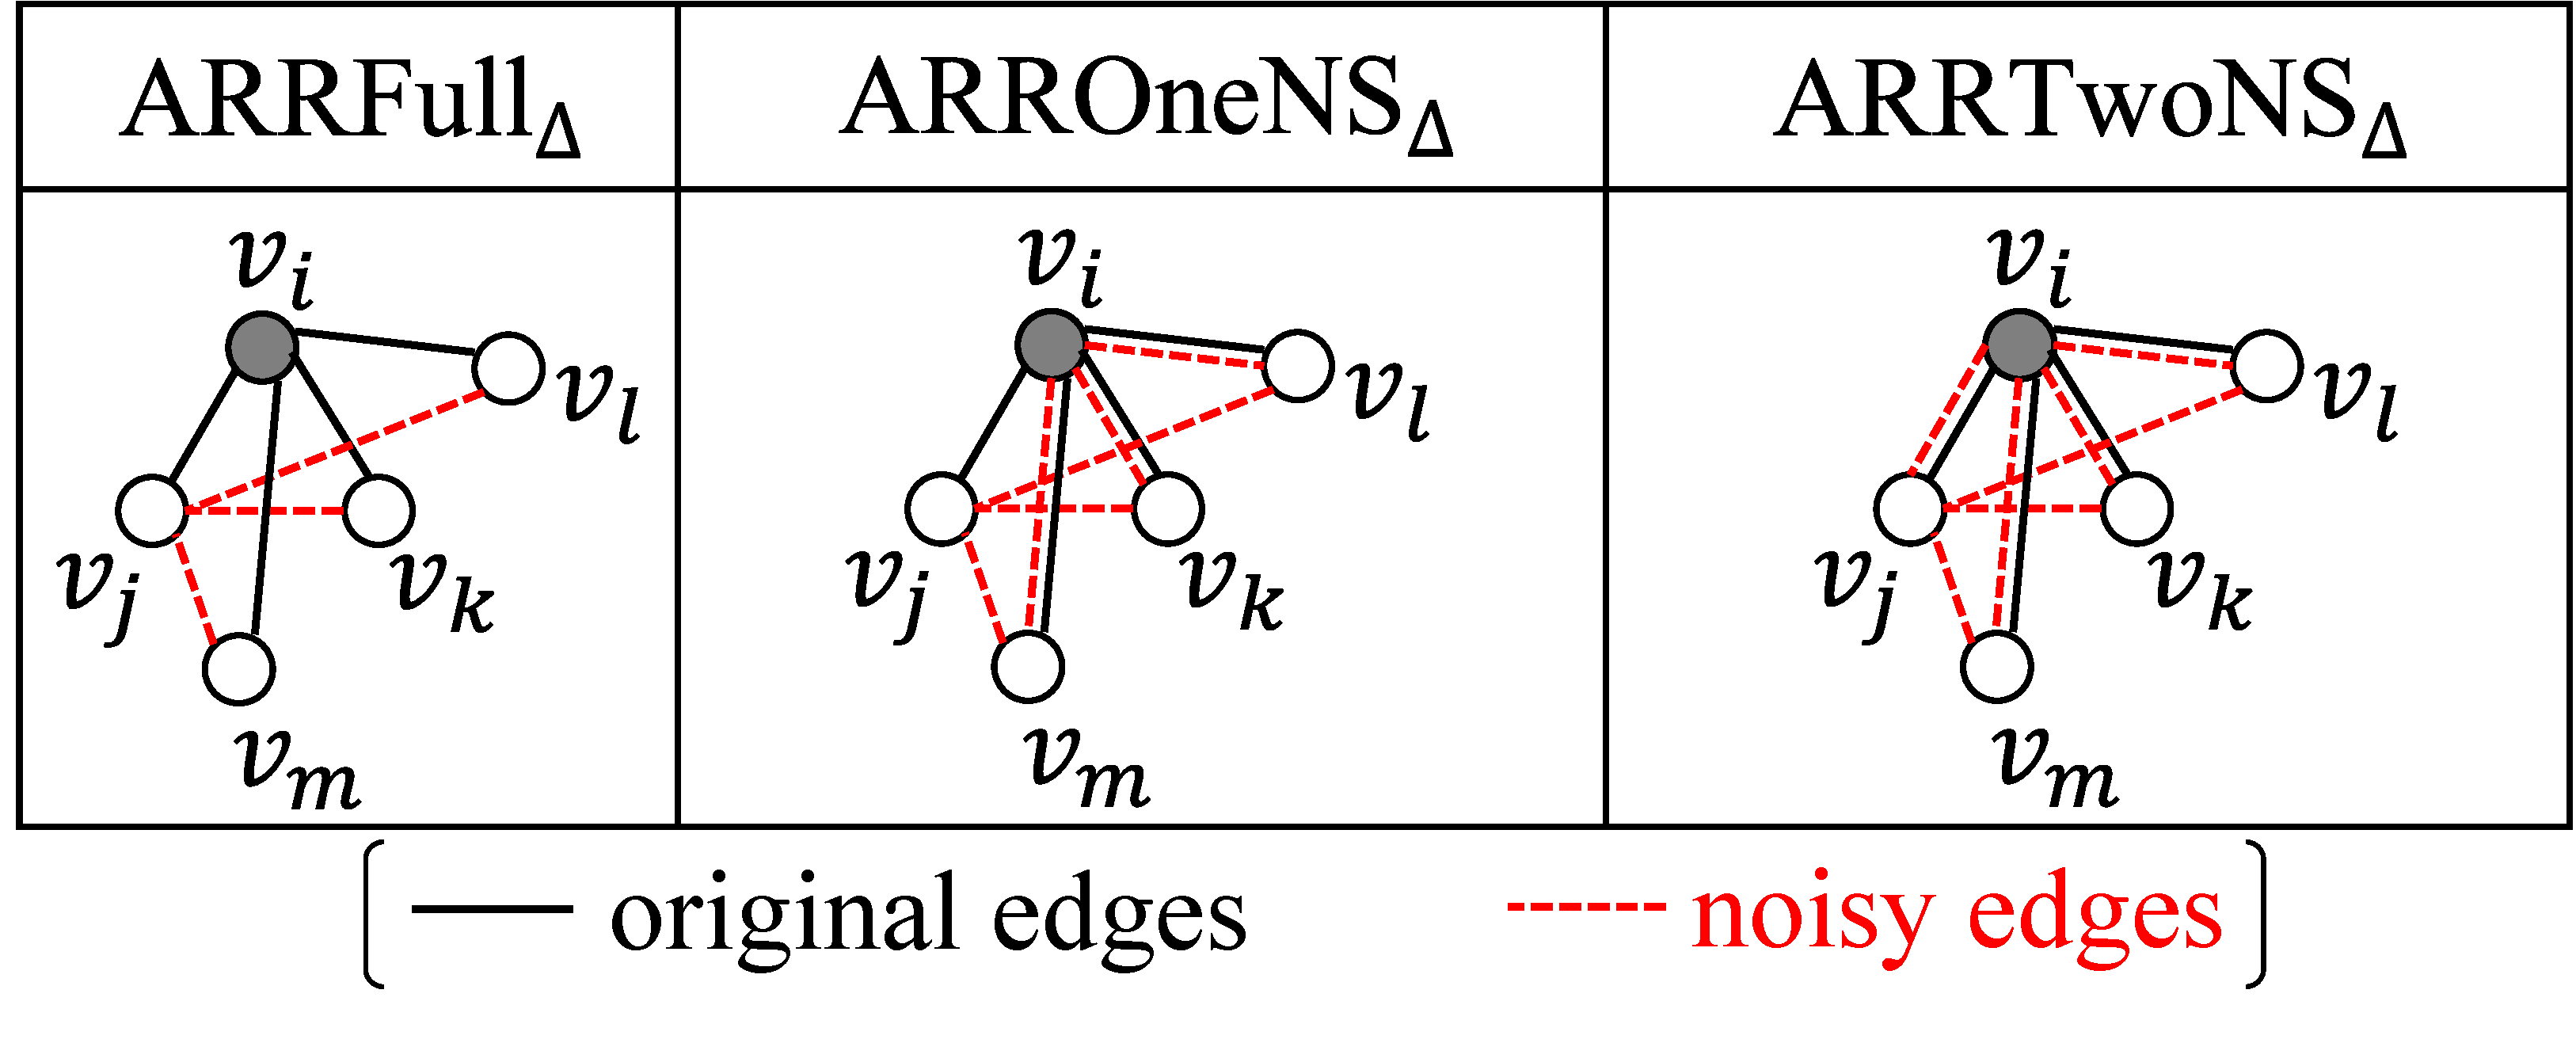
\includegraphics[width=0.78\linewidth]{fig/double_clipping.pdf}
  \vspace{-4mm}
  \caption{Noisy triangles involving edge $(v_i,v_j)$ counted by user $v_i$ ($j<k,l,m<i$).} 
  \label{chap2-fig:reduce_noisy_triangles}
%\end{figure}
\vspace{2mm}
%\begin{figure}[t]
  \centering
  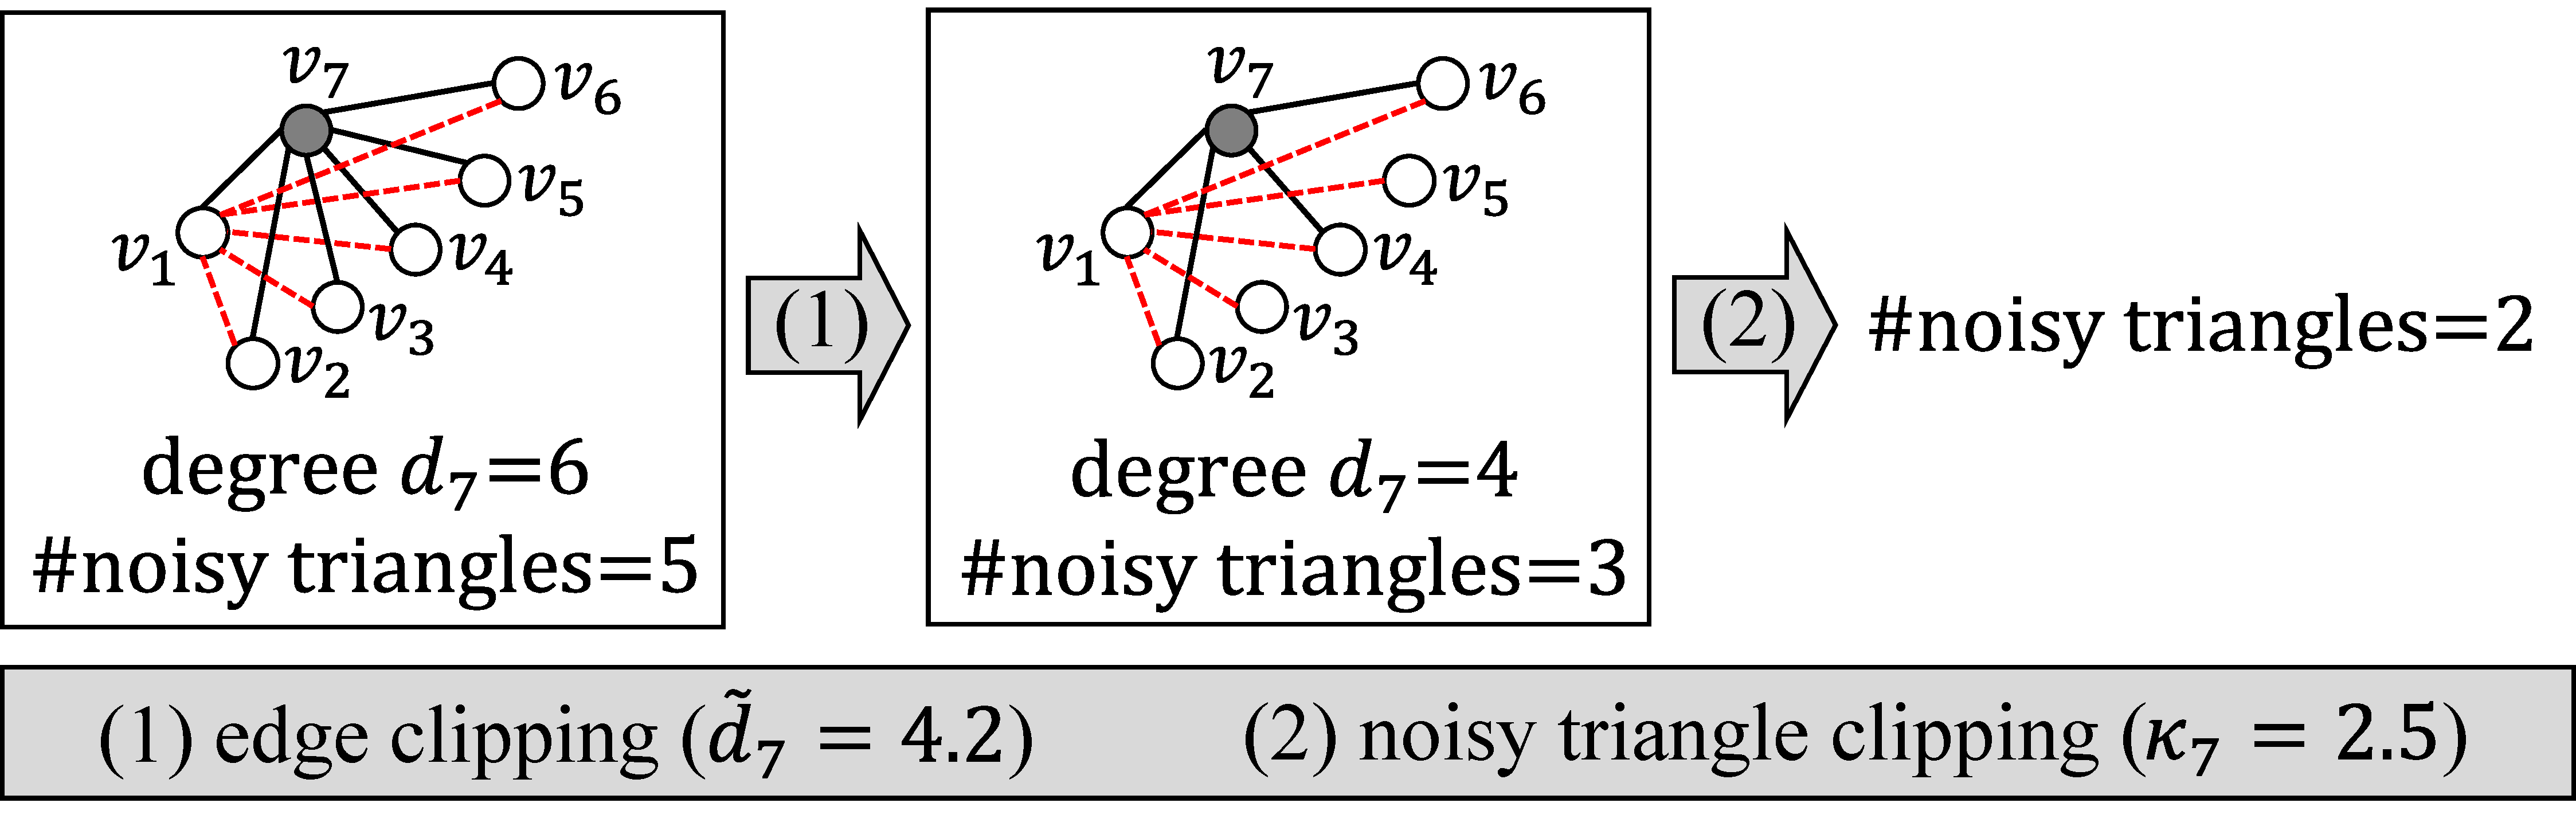
\includegraphics[width=0.99\linewidth]{fig/clip_overview.pdf}
  \vspace{-4mm}
  \caption{Overview of double clipping applied to edge ($v_1,v_7$).} 
  \label{chap2-fig:double-clip_overview}
\end{figure}

% To address the first and second issues explained above, we introduce an edge clipping and triangle clipping, respectively. 
To address these two issues, 
%(i.e., the leakage of $d_i$ and the excess of the noisy triangle count), 
we propose a double clipping technique, which is explained below. 
% which consists of an \textit{adaptive edge clipping} and \textit{noisy triangle clipping}. 

\smallskip
\noindent{\textbf{Algorithm Overview.}}~~Figure~\ref{chap2-fig:double-clip_overview} shows 
% its overview. 
the overview of our double clipping, which consists of an 
% \textit{adaptive edge clipping} 
\textit{edge clipping} 
and \textit{noisy triangle clipping}. 
% The adaptive edge clipping 
The edge clipping 
addresses the first issue (i.e., leakage of $d_i$) 
as follows. 
% by borrowing the idea of adaptive clipping \cite{Andrew_arXiv21,Pichapati_arXiv19} 
% in DP-SGD (Differentially Private Stochastic Gradient Descent). 
% which privately estimates an appropriate clipping threshold in DP-SGD (Stochastic Gradient Descent) \cite{Abadi_CCS16} with DP. 
% Specifically, it 
It privately computes 
a noisy version of 
$d_i$ (denoted by $\td_i$) with edge LDP. 
% Let $\td_i \in \nnreals$ be the private value of $d_i$. 
% user $v_i$ 
% adds the Laplacian noise and some positive constant $\eta \in \nnreals$ to $d_i$ to provide edge LDP 
% and 
Then it 
%performs edge clipping 
%(a.k.a. graph projection \cite{Day_SIGMOD16,Ding_TKDE21,Kasiviswanathan_TCC13,Raskhodnikova_arXiv15}), which 
removes some neighbors from a neighbor list $\bma_i$ so that the degree of $v_i$ never exceeds 
% the private estimate of $d_i$. 
% the private value of $d_i$ 
% (denoted by $\td_i \in \nnreals$). 
% (denoted by $\td_i$). 
the noisy degree $\td_i$. 
This removal process is also known as graph projection \cite{Day_SIGMOD16,Ding_TKDE21,Kasiviswanathan_TCC13,Raskhodnikova_arXiv15}. 
% This kind of technique is called adaptive clipping \cite{Andrew_arXiv21,Pichapati_arXiv19} 
% in DP-SGD (Stochastic Gradient Descent) \cite{Abadi_CCS16} because it privately estimates an appropriate clipping threshold with DP. 
% Adaptive edge clipping 
Edge clipping 
is 
% also 
used in \cite{Imola_USENIX21} to obtain a 
% private value of 
noisy version of 
% the maximum degree 
$d_{max}$. 
%(though ours is to obtain a noisy version of $d_i$). 

% The triangle clipping addresses the second issue (i.e., excess of the noisy triangle count) by reducing the noisy triangle count so that it never exceeds a 
% user-dependent threshold $\kappa_i \in \nnints$. 
The main novelty in our double clipping lies at the \textit{noisy triangle clipping} to address the second issue (i.e., excess of the noisy triangle count). 
% Note that 
This issue appears 
% only 
when 
% each edge is sampled and 
we attempt to reduce the global sensitivity by using 
a very small sampling probability for each edge. 
% value of $\mu$ in the ARR.  
% using a stochastic algorithm such as the ARR. 
Therefore, the noisy triangle clipping has not been studied in the existing works on private triangle counting 
% \cite{Ding_TKDE21,Imola_USENIX21,Karwa_PVLDB11,Kasiviswanathan_TCC13,Song_arXiv18,Sun_CCS19,Ye_ICDE20,Ye_TKDE21,Zhang_SIGMOD15}, 
\cite{Ding_TKDE21,Imola_USENIX21,Karwa_PVLDB11,Kasiviswanathan_TCC13,Sun_CCS19,Ye_ICDE20,Ye_TKDE21,Zhang_SIGMOD15}, 
because they do not apply a sampling technique. 

Our noisy triangle clipping reduces the noisy triangle count so that it never exceeds a 
user-dependent clipping threshold 
$\kappa_i \in \nnreals$. 
% $\kappa_i = \lambda_i \mu^* \td_i$, where $\lambda_i \in \nats$. 
% We call $\kappa_i$ and $\lambda_i$ the \textit{clipping threshold} and \textit{clipping coefficient}, respectively. 
Then a crucial issue is how to set 
an appropriate 
% clipping 
threshold 
$\kappa_i$. 
We theoretically analyze the probability that the noisy triangle count exceeds $\kappa_i$ 
(referred to as the \textit{triangle excess probability}) 
as a function of 
the ARR parameter $\mu$ and the 
% private value $\td_i$ of $d_i$. 
noisy degree $\td_i$. 
% of user $v_i$. 
Then we set $\kappa_i$ so that 
the triangle excess probability 
% the probability 
is very small ($=10^{-6}$ in our experiments). 

We use the clipping threshold $\kappa_i$ as a global sensitivity. 
% of the Laplacian noise. 
Note that $\kappa_i$ provides edge LDP because $\td_i$ provides edge LDP, 
% and $\kappa_i$ depends on only $\mu$ and $\td_i$ 
i.e., immunity to post-processing \cite{DP}. 
$\kappa_i$ is also very small when $\mu \ll 1$, as it is determined based on $\mu$. 

% We also emphasize that our double clipping does \textit{not} assume that $d_{max}$ is public, because it privately computes $\td_i$. 
% by adaptive edge clipping.

\subsection{Algorithms}
\label{chap2-sub:algorithms}
Algorithm~\ref{chap2-alg:clip} shows our double clipping algorithm. 
All the processes are run by user $v_i$ at the second round. 
Thus, there is no interaction with the server in Algorithm~\ref{chap2-alg:clip}.

\setlength{\algomargin}{5mm}
\begin{algorithm}[t]
  \SetAlgoLined
  \KwData{Neighbor list $\bma_i \in \{0,1\}^n$, privacy budget
  $\epsilon_0 \in \nnreals$ 
  $\mu \in [0,\frac{e^{\epsilon_1}}{e^{\epsilon_1} + 1}]$, 
  %$\eta \in \nnreals$.
  $\alpha \in \nnreals$, 
  $\beta \in \nnreals$.
  }
  \KwResult{$\hw_i$.}
  $\mu^* \leftarrow \mu$, $\mu^2$, and $\mu^3$ in F, O, and T, respectively\;
  \tcc{Edge clipping.}
  %$\td_i = \max\{d_i + \Lap(\frac{1}{\epsilon_0}) + \eta$, 0\}\;
  $\td_i = \max\{d_i + \Lap(\frac{1}{\epsilon_0}) + \alpha$, 0\}\;
  \tcc{Remove $d_i - \lfloor \td_i \rfloor$ neighbors if $d_i > \td_i$.}
  $\bma_i \leftarrow \texttt{GraphProjection}(\bma_i, \td_i)$\;
  \tcc{Noisy triangle clipping.}
  \For{$j$ \rm{such that} $a_{i,j} = 1$ \rm{and} $j<i$}{
    $t_{i,j} \leftarrow |\{(v_i,v_j,v_k) : a_{i,k} = 1, (v_j,v_k) \in M_i, j<k<i \}|$\;
  }
%  \tcc{Calculate $\kappa_i$ such that $\kappa_i \in [\mu^* \td_i, \td_i]$.}
   \tcc{Calculate $\kappa_i \in [\mu^* \td_i, \td_i]$ s.t. the triangle excess probability is $\beta$ or less.}
%  \tcc{Calculate $\lambda_i \in \nats$ such that the triangle excess probability is $\beta$ or less.}
  $\kappa_i \leftarrow \texttt{ClippingThreshold}(\mu, \td_i, \beta)$\;
%  $\lambda_i \leftarrow \texttt{ClippingThreshold}(\mu, \td_i, \beta)$\;
%   $\kappa_i \leftarrow \lambda_i \mu^* \td_i$\;
  $t_i \leftarrow \sum_{a_{i,j} = 1, j<i} \min \{t_{i,j}, \kappa_i\}$\;
  $s_i \leftarrow |\{(v_i,v_j,v_k) : a_{i,j} = a_{i,k} = 1, j<k<i\}|$\;
  $w_i \leftarrow t_i - \mu^* \rho s_i$\;
  $\hw_i \leftarrow w_i + \Lap(\frac{\kappa_i}{\epsilon_2})$\;
  \KwRet{$\hw_i$}
  \caption{Our double clipping algorithm. 
  ``F'', ``O'', ``T'' are shorthands for 
  \AlgOne{}, \AlgTwo{}, and \AlgThree{}, respectively.
  All the processes are run by user $v_i$.
  }\label{chap2-alg:clip}
\end{algorithm}

\smallskip
\noindent{\textbf{Edge Clipping.}}~~The edge clipping appears in lines 2-3 of Algorithm~\ref{chap2-alg:clip}. 
It uses a privacy budget $\epsilon_0 \in \nnreals$. 
% for privately computing $d_i$. 

In line 2, user $v_i$ adds the Laplacian noise $\Lap(\frac{1}{\epsilon_0})$ to her degree $d_i$. 
Since adding/removing one edge changes $d_i$ by at most $1$, this process provides $\epsilon_0$-edge LDP. 
$v_i$ also adds some non-negative constant 
% $\eta \in \nnreals$ 
$\alpha \in \nnreals$ 
to $d_i$. 
We add this value so that edge removal (in line 3) occurs with a very small probability; 
e.g., in our experiments, we set $\alpha = 150$, where 
% when $\epsilon_0 = 0.1$ and $\alpha = 150$, 
edge removal occurs with probability $1.5 \times 10^{-7}$ when $\epsilon_0 = 0.1$. 
A similar technique is introduced in \cite{Sun_CCS19} to provide ($\epsilon, \delta)$-DP \cite{DP} with small $\delta$. 
The difference between ours and \cite{Sun_CCS19} is that we perform edge clipping 
% (graph projection) 
to always provide $\epsilon$-DP; i.e., $\delta = 0$.
Let $\td_i \in \nnreals$ be the noisy degree of $v_i$.

In line 3, user $v_i$ calls the function \texttt{GraphProjection}, which performs graph projection as follows; 
if $d_i > \td_i$, randomly remove $d_i - \lfloor \td_i \rfloor$ neighbors from $\bma_i$; otherwise, do nothing. 
Consequently, the degree 
% $d_i$ 
of $v_i$ never exceeds $\td_i$. 

\begin{table*}[t]
  \centering
  \begin{tabular}{|l|c|c|c|}
    \hline
    & \AlgOne & \AlgTwo & \AlgThree \\ \hline
    Privacy 
    & \multicolumn{3}{|c|}{$(\epsilon_0 + \epsilon_1 + \epsilon_2)$-edge LDP and $(\epsilon_0 + \epsilon_1 + \epsilon_2)$-relationship DP} \\ \hline
    %& $\epsilon_0 + \epsilon_1 + \epsilon_2$ & $\epsilon_0 + \epsilon_1 + \epsilon_2$ &
    %$\epsilon_0 + \epsilon_1 + \epsilon_2$ \\ \hline
    Expected $l_2$ loss 
    % & $\frac{2 C_4(G) + S_2(G)}{\mu(1-e^{-\epsilon_1})^2}$ + $\frac{2 \sum_{i=1}^n \kappa_{i}^2}{\mu^2 (1-e^{-\epsilon_1})^2 \epsilon_2^2}$
    % & $O\left(\frac{n d_{max}^3}{\mu(1-e^{-\epsilon_1})^2} + \frac{2 \sum_{i=1}^n \lambda_{i}^2 \td_i^2}{(1-e^{-\epsilon_1})^2 \epsilon_2^2}\right)$
    & $O\left(\frac{n d_{max}^3}{\mu(1-e^{-\epsilon_1})^2} + \frac{2 \sum_{i=1}^n \kappa_{i}^2}{\mu^2(1-e^{-\epsilon_1})^2 \epsilon_2^2}\right)$
    % & $\frac{\mu(12 S_3(G) + 6 P_3(G)) + 6 S_2(G)}{\mu^2(1-e^{-\epsilon_1})^2}$ + $\frac{2 \sum_{i=1}^n \kappa_{i}^2}{\mu^4 (1-e^{-\epsilon_1})^2 \epsilon_2^2}$
    % & $O\left(\frac{n d_{max}^2}{\mu^2(1-e^{-\epsilon_1})^2} + \frac{2 \sum_{i=1}^n \lambda_{i}^2 \td_i^2}{(1-e^{-\epsilon_1})^2 \epsilon_2^2} \right)$
    & $O\left(\frac{n d_{max}^2}{\mu^2(1-e^{-\epsilon_1})^2} + \frac{2 \sum_{i=1}^n \kappa_{i}^2}{\mu^4 (1-e^{-\epsilon_1})^2 \epsilon_2^2} \right)$
    % & $\frac{\mu^2 (12 S_3(G) + 6 P_3(G)) + 6 S_2(G)}{\mu^3(1-e^{-\epsilon_1})^2}$ + $\frac{2 \sum_{i=1}^n \kappa_{i}^2}{\mu^6 (1-e^{-\epsilon_1})^2 \epsilon_2^2}$ \\ \hline
    % & $O\left(\frac{n d_{max}^2}{\mu^3(1-e^{-\epsilon_1})^2} + \frac{2 \sum_{i=1}^n \lambda_{i}^2 \td_i^2}{(1-e^{-\epsilon_1})^2 \epsilon_2^2} \right)$ \\ \hline
    & $O\left(\frac{n d_{max}^2}{\mu^3(1-e^{-\epsilon_1})^2} + \frac{2 \sum_{i=1}^n \kappa_{i}^2}{\mu^6 (1-e^{-\epsilon_1})^2 \epsilon_2^2} \right)$ \\ \hline
    % $l_2$ loss of emp 
    % & $\frac{2 C_4(G) + S_2(G)}{\mu_F(1-e^{-\epsilon_1})^2}$
    % & $\frac{\mu_O(12 S_3(G) + 6 P_3(G)) + 6 S_2}{\mu_O^2(1-e^{-\epsilon_1})^2}$
    % & $\frac{\mu_T^2 (12 S_3(G) + 6 P_3(G)) + 6 S_2}{\mu_T^3(1-e^{-\epsilon_1})^2}$ \\ \hline
    % $l_2$ loss of \Lap{} 
    % & $\frac{2 \sum_{i=1}^n \kappa_{i,F}^2}{\mu_F^2 (1-e^{-\epsilon_1})^2 \epsilon_2^2}$
    % & $\frac{2 \sum_{i=1}^n \kappa_{i,O}^2}{\mu_F^2 (1-e^{-\epsilon_1})^2 \epsilon_2^2}$
    % & $\frac{2 \sum_{i=1}^n \kappa_{i,T}^2}{\mu_F^2 (1-e^{-\epsilon_1})^2 \epsilon_2^2}$ \\ \hline
    $\text{Cost}_{DL}$ & 
    $\mu n^2 \log n$ 
    % $\mu e^{-\epsilon_1} n^2 \log n$ 
    % $\mu_F e^{-\epsilon_1} n(n-1) \log n$ 
    % $(n(n-1) \mu_F \rho + |E| \mu_F (1 - \rho)) \log n$ 
    & 
    $\mu^2 n^2 \log n$ 
    % $\mu^2 e^{-\epsilon_1} n^2 \log n$ 
    % $\mu_O^2 e^{-\epsilon_1} n(n-1) \log n$ 
    & 
    $\mu^3 n^2 \log n$ 
    % $\mu^3 e^{-\epsilon_1} n^2 \log n$ 
    % $\mu_T^3 e^{-\epsilon_1} n(n-1) \log n$ 
    \\ \hline
    $\text{Cost}_{UL}$ & 
    $\mu n \log n$ & $\mu n \log n$ & $\mu n \log n$ 
    % $\mu e^{-\epsilon_1} n \log n$ & $\mu e^{-\epsilon_1} n \log n$ & $\mu e^{-\epsilon_1} n \log n$ 
    \\ \hline
  \end{tabular}
  \vspace{-2mm}
  \caption{Performance guarantees 
  %Privacy, expected $l_2$ loss, and download/upload cost 
  of our three algorithms with double clipping when the edge removal and triangle removal do not occur. 
  %($C_4$: \#$4$-cycles, $P_3$: \#$3$-paths, $S_k$: \#$k$-stars). 
  %($\lambda_i$: clipping coefficient, $\td_i$: noisy degree).
  The expected $l_2$ loss assumes that $\mu$ is small. 
  The download (resp.~upload) cost is an upper-bound in (\ref{chap2-eq:CostDL_F}) 
  %, (\ref{chap2-eq:CostDL_O}), (\ref{chap2-eq:CostDL_T}), 
  (resp.~(\ref{chap2-eq:CostUL_proposal})).
  %approximation when $d_{max} \ll n$. 
  %the graph $G$ is sparse.
  }
  \label{chap2-tab:privacy_utility_cost}
\end{table*}

\smallskip
\noindent{\textbf{Noisy Triangle Clipping.}}~~The noisy triangle clipping appears in lines 4-11 of Algorithm~\ref{chap2-alg:clip}. 

% First, 
In lines 4-6, 
user $v_i$ calculates the number $t_{i,j} \in \nnints$ of noisy triangles ($v_i, v_j, v_k$) ($j<k<i$) involving $(v_i,v_j)$ 
(as shown in Figure~\ref{chap2-fig:reduce_noisy_triangles}). 
%such that only one edge ($v_j, v_k$) is noisy 
% for her neighbor $v_j$. 
% (lines 4-6). 
Note that the total number $t_i$ of noisy triangles of $v_i$ can be expressed as: 
$t_i = \sum_{a_{i,j}=1, j<i} t_{i,j}$. 
In line 7, $v_i$ calls the function \texttt{ClippingThreshold}, which calculates a clipping threshold 
% $\kappa_i$ 
$\kappa_i \in [\mu^* \td_i, \td_i]$ 
($\mu^* = \mu$, $\mu^2$, and $\mu^3$ in 
``F'', ``O'', and ``T'', respectively) 
based on the ARR parameter $\mu$ and the noisy degree $\td_i$ so that 
% $\kappa_i \in [\mu^* \td_i, \td_i]$ 
% ($\mu^* = \mu$, $\mu^2$, and $\mu^3$ in 
% ``F'', ``O'', and ``T'', respectively) 
% and 
the triangle excess probability does not exceed some constant $\beta \in \nnreals$. 
% $\kappa_i$ takes a value between $\mu^* \td_i$ and $\td_i$; i.e., $\kappa_i \in [\mu^* \td_i, \td_i]$. 
We explain how to calculate 
% $\kappa_i$ from $\mu$ and $\td_i$ 
the triangle excess probability 
in Section~\ref{chap2-sub:clip_theoretical_analysis}. 
% in detail. 
In line 8, $v_i$ calculates the total number $t_i$ of noisy triangles by summing up $t_{i,j}$, with the exception that $v_i$ adds $\kappa_i$ 
%(rather than $t_{i,j}$) 
if $t_{i,j} > \kappa_i$. 
%$t_{i,j}$ exceeds $\kappa_i$. 
In other words, triangle removal occurs 
% when 
if 
$t_{i,j} > \kappa_i$. 
% Consequently, 
Then, 
the number 
% $t_{i,j}$ 
of noisy triangles involving $(v_i,v_j)$ never exceeds $\kappa_i$. 

Lines 9-11 in Algorithm~\ref{chap2-alg:clip} are the same as lines 12-14 in Algorithm~\ref{chap2-alg:unify}, except that 
the global sensitivity in the former (resp.~latter) is $\kappa_i$ (resp.~$d_{max}$). 
% the global sensitivity in Algorithm~\ref{chap2-alg:clip} is $\kappa_i$. 
Line 11 in Algorithm~\ref{chap2-alg:clip} provides $\epsilon_2$-edge LDP because the number of triangles involving $(v_i,v_j)$ is now upper-bounded by $\kappa_i$. 

\smallskip
\noindent{\textbf{Our Entire Algorithms with Double Clipping.}}~~We can run our algorithms \AlgOne{}, \AlgTwo{}, \AlgThree{} with double clipping just by replacing lines 11-14 in Algorithm~\ref{chap2-alg:unify} with lines 2-11 in Algorithm~\ref{chap2-alg:clip}. 
That is, after calculating $\hw_i$ by Algorithm~\ref{chap2-alg:clip}, $v_i$ uploads $\hw_i$ to the server. 
Then the server calculates an estimate of $f_\triangle(G)$ as $\hf_\triangle(G) = \frac{1}{\mu^*(1-\rho)}\sum_{i=1}^n \hw_i$. 
%as in line 17 of Algorithm~\ref{chap2-alg:unify}. 
% where $\mu^* = \mu$, $\mu^2$, and $\mu^3$ in 
% ``F'', ``O'', and ``T'', respectively). 

We also note that the input $d_{max}$ in Algorithm~\ref{chap2-alg:unify} is no longer necessary thanks to the edge clipping; i.e., our entire algorithms with double clipping do not assume that $d_{max}$ is public. 
% , because $v_i$ privately calculates $d_i$ by edge clipping.

\subsection{Theoretical Analysis}
\label{chap2-sub:clip_theoretical_analysis}
% \paragraph{Privacy}
% \smallskip
We now perform a theoretical analysis on the privacy and utility of our double clipping. 
% All the proofs appear in \arxiv{Appendix~\ref{chap2-sec:proof_double_clip}}\conference{the full version \cite{Imola_arXiv22}}. 

\smallskip
\noindent{\textbf{Privacy.}}~~We begin with the privacy guarantees:
% Our algorithms with double clipping have the following privacy guarantees:
\begin{theorem}\label{chap2-thm:privacy_DC}
  For $i \in [n]$, 
  let $\calR_i^1, \calR_i^2(M_i)$ be the randomizers used by user $v_i$ in
  rounds $1$ and $2$ of our algorithms with double clipping (Algorithms~\ref{chap2-alg:unify} and \ref{chap2-alg:clip}). 
  Let $\calR_i(\bma_i) = (\calR_i^1(\bma_i), \calR_i^2(M_i)(\bma_i))$ 
  be the composition of the two randomizers. 
  Then,
  $\calR_i$ satisfies $(\epsilon_0 + \epsilon_1 + \epsilon_2)$-edge LDP, 
  %for $i \in [n]$, 
  and $(\calR_1,
  \ldots, \calR_n)$ satisfies $(\epsilon_0 + \epsilon_1 + \epsilon_2)$-relationship DP.
\end{theorem}

\smallskip
\noindent{\textbf{Utility.}}~~Next, we show the triangle excess probability: 
% the probability that the noisy triangle count $t_{i,j}$ exceeds $\kappa_i$:

\begin{theorem}\label{chap2-thm:triangle_excess}
%Let $\mu^* = \mu_F$ and $\mu_O^2$ in \AlgOne{} and \AlgTwo{}, respectively. 
%In \AlgOne{} and \AlgTwo{}, 
%In \AlgOne{}, \AlgTwo{}, \AlgThree{}, 
% Let $\mu_F, \mu_O, \mu_T \in [0,\frac{e^{\epsilon}}{e^{\epsilon_1} + 1}]$. 
% For $i \in [n]$, let $\td_i \in \nnreals$ be a noisy degree of user $v_i$ output by edge clipping. 
% Let $\kappa_i$
In Algorithm~\ref{chap2-alg:clip}, the triangle excess probability (i.e., probability that the number of noisy triangles $t_{i,j}$ involving edge $(v_i, v_j)$ exceeds a clipping threshold $\kappa_i$) is:
  \begin{align}
    \hspace{-1mm} \Pr(t_{i,j} > \kappa_i) &\leq \textstyle{\exp \left[-\td_i D \left(\frac{\kappa_i}{\td_i} \parallel \mu \right) \right]} \label{chap2-eq:AlgI_clip_bound} \\
    \hspace{-1mm} \Pr(t_{i,j} > \kappa_i) &\leq \textstyle{\exp \left[-\td_i D \left(\frac{\kappa_i}{\td_i} \parallel \mu^2 \right) \right]} \label{chap2-eq:AlgII_clip_bound}\\
%   \end{align}
%   \begin{align}
    \hspace{-1mm} \Pr(t_{i,j} > \kappa_i) &\leq 
    \textstyle{\mu \exp \left[-\td_i D \left(\frac{\max\{\kappa_i,\mu^2 \td_i\}}{\td_i} \parallel \mu^2 \right) \right]}
    % \begin{cases}
    %     \mu_T \exp \left[-\td_i D \left(\frac{\kappa_i}{\td_i} \parallel \mu_T^2 \right) \right]   &   \mathrm{(if}~ \kappa_i \geq \mu_T^2 \td_i)\\
    %     \mu_T   &   \mathrm{(if}~ \mu_T^3 \td_i \leq \kappa_i < \mu_T^2 \td_i),
    % \end{cases}
    \label{chap2-eq:AlgIII_clip_bound}
  \end{align}
  in \AlgOne{}, \AlgTwo{}, and \AlgThree{}, respectively, 
  where 
  % $\mu^* = \mu_F$ and $\mu_O^2$ in \AlgOne{} and \AlgTwo{}, respectively, and 
  $D(p_1 \parallel p_2)$ is the Kullback-Leibler divergence between two Bernoulli distributions; i.e., 
  %$D(p_1 \parallel p_2) = p_1 \log \frac{p_1}{p_2} + (1-p_1) \log \frac{1-p_1}{1-p_2}$.
  %with $p_1$ and $p_2$:
  %the Bernoulli($p_1$) and Bernoulli($p_2$) distribution; 
\begin{align*}
    \textstyle{D(p_1 \parallel p_2) = p_1 \log \frac{p_1}{p_2} + (1-p_1) \log \frac{1-p_1}{1-p_2}.}
\end{align*}
\end{theorem}
In all of (\ref{chap2-eq:AlgI_clip_bound}), (\ref{chap2-eq:AlgII_clip_bound}), and (\ref{chap2-eq:AlgIII_clip_bound}), we use the Chernoff bound, which is known to be reasonably tight \cite{Arratia_BMB89}. 

\smallskip
\noindent{\textbf{Setting $\kappa_i$.}}~~The function \texttt{ClippingThreshold} in Algorithm~\ref{chap2-alg:clip} sets a clipping threshold $\kappa_i$ of user $v_i$ based on Theorem~\ref{chap2-thm:triangle_excess}. 
Specifically, we set $\kappa_i = \lambda_i \mu^* \td_i$, where $\lambda_i \in \nats$, and calculate $\lambda_i$ as follows. 
We initially set $\lambda_i = 1$ and keep increasing $\lambda_i$ by $1$ 
% initially set $\kappa_i = \mu^* \td_i$ and keep increasing $\kappa_i$ by $\mu^* \td_i$ 
until the upper-bound (i.e., right-hand side of (\ref{chap2-eq:AlgI_clip_bound}), (\ref{chap2-eq:AlgII_clip_bound}), or (\ref{chap2-eq:AlgIII_clip_bound})) is smaller than or equal to the triangle excess probability $\beta$. 
In our experiments, we set $\beta = 10^{-6}$. 
% We call $\lambda_i$ the \textit{clipping coefficient} of $v_i$. 

\smallskip
\noindent{\textbf{Large $\kappa_i$ of \AlgThree{}.}}~~By 
% In our experiments, we set $\mu$ so that $\mu$ in \AlgOne{} is equal to $\mu^2$ in \AlgTwo{} and also equal to $\mu^3$ in \AlgThree{}. 
% Then by 
(\ref{chap2-eq:AlgI_clip_bound}) and (\ref{chap2-eq:AlgII_clip_bound}), the upper-bound on the triangle excess probability is the same between \AlgOne{} and \AlgTwo{}. 
% However, 
In contrast, 
\AlgThree{} has a larger upper-bound. 
For example, 
when $\kappa_i = 15 \mu^* \td_i$, $\mu^* = 10^{-3}$, and $\td_i=1000$, 
the right-hand sides of (\ref{chap2-eq:AlgI_clip_bound}), (\ref{chap2-eq:AlgII_clip_bound}), and (\ref{chap2-eq:AlgIII_clip_bound}) are $2.5 \times 10^{-12}$, $2.5 \times 10^{-12}$, and $3.3 \times 10^{-2}$, respectively. 
Consequently, \AlgThree{} has a larger global sensitivity $\kappa_i$ for the same value of $\beta$.

% \smallskip
% \noindent{\textbf{\AlgTwo{} vs. \AlgThree{}.}}~~Now we explain the reason that \AlgTwo can reduce the global sensitivity more effectively than \AlgThree (as described in Section~\ref{chap2-sub:algorithms_overview}).  
% using Figure~\ref{chap2-fig:reduce_noisy_triangles}. 
% As with \AlgOne, 
We can explain a large global sensitivity $\kappa_i$ of \AlgThree{} as follows. 
The number $t_{i,j}$ of noisy triangles involving $(v_i,v_j)$ in 
\AlgOne{} is expected to be around $\mu d_i$ because one noisy edge is in each noisy triangle (as in Figure~\ref{chap2-fig:reduce_noisy_triangles}) and all noisy edges are independent. 
For the same reason, $t_{i,j}$ in \AlgTwo{} is expected to be around $\mu^2 d_i$.  
% \AlgTwo{} is expected to be around $\mu_O^2 d_i$ because two noisy edges are in each noisy triangle (as in Figure~\ref{chap2-fig:reduce_noisy_triangles}) and all noisy edges are independent. 
% 
However, 
% the number of noisy triangles involving $(v_i,v_j)$ 
$t_{i,j}$ in \AlgThree{} is \textit{not} expected to be around $\mu^3 d_i$, because all the noisy triangles have noisy edge $(v_i,v_j)$ in common (as in Figure~\ref{chap2-fig:reduce_noisy_triangles}). 
Then, 
% the expected noisy triangle count 
the expectation of $t_{i,j}$ 
largely depends on the presence/absence of the noisy edge $(v_i,v_j)$; i.e., if noisy edge $(v_i,v_j)$ exists, 
it is $\mu^2 d_i$; otherwise, $0$. 
% Consequently, 
% the noisy triangle count (i.e., global sensitivity) 
% the global sensitivity 
Thus, 
$\kappa_i$ 
cannot be effectively reduced by double clipping. 
% Section~\ref{chap2-sub:clip_theoretical_analysis} shows a more formal result on this. 

\smallskip
\noindent{\textbf{Summary.}}~~The 
% privacy, expected $l_2$ loss, download/upload cost 
performance guarantees 
of our three algorithms with double clipping can be summarized in Table~\ref{chap2-tab:privacy_utility_cost}.

% The expected $l_2$ loss can be expressed $O(n d_{max}^3)$, $O(n d_{max}^2)$, and $O(n d_{max}^2)$, 
% For the $l_2$ loss, 
The first and second terms of the expected 
$l_2$ loss are the $l_2$ loss of empirical estimation and that of the Laplacian noise, respectively. 
For small 
% $\mu_F$ ($=\mu_O^2 = \mu_T^3$), 
$\mu$, 
the $l_2$ loss of empirical estimation can be expressed as $O(n d_{max}^3)$, $O(n d_{max}^2)$, and $O(n d_{max}^2)$ in \AlgOne{}, \AlgTwo{}, \AlgThree{}, respectively, as explained in Section~\ref{chap2-sub:algorithms_theoretical_analysis}. 
% (when we regard $\epsilon_1$ and $\epsilon_2$ as constants). 
% The large $l_2$ loss of \AlgOne{} is caused by the number $C_4$ of $4$-cycles that is written as $O(n d_{max}^3)$. 
The $l_2$ loss of the Laplacian noise is 
$O(\sum_{i=1}^n \kappa_i^2)$, 
% $O(\sum_{i=1}^n \lambda_i^2 \td_i^2)$, 
which is much smaller than $O(n d_{max}^2)$. 
% when $\lambda_i$ is small. 
Thus, our \AlgTwo{} that effectively reduces $\kappa_i$ provides the smallest error, 
% for a large graph or dense graph where $C_4$ is large, 
as shown in our experiments.

We also note that 
both the space and the time complexity to compute and send $M_i$ in our algorithms 
% time and space complexity of 
% our algorithms at the server side 
are $O(\mu^* n^2)$ (as $|E'| =  O(\mu^* n^2)$), which is much smaller than \cite{Imola_USENIX21} ($=O(n^2)$). 


\section{Experiments}
\label{chap2-sec:experiments}

% Based on the theoretical results in Sections~\ref{chap2-sub:algorithms_theoretical_analysis} and \ref{chap2-sub:clip_theoretical_analysis}, we would like to pose the following questions:
To evaluate each component of our algorithms in Sections~\ref{chap2-sec:algorithms} and \ref{chap2-sec:double_clip} as well as our entire algorithms (i.e., \AlgOne, \AlgTwo, \AlgThree with double clipping), we pose the following three research questions:
%\begin{enumerate}
\begin{description}[leftmargin=9.75mm]
% \begin{itemize}[leftmargin=9.7mm]
    \item[RQ1.] 
    %\item 
    How do our three triangle counting algorithms 
    (i.e., \AlgOne, \AlgTwo, \AlgThree) in Section~\ref{chap2-sec:algorithms} compare with each other in terms of accuracy?
    \item[RQ2.] 
    %\item 
    How much does our double clipping technique in Section~\ref{chap2-sec:double_clip} decrease the estimation error?
    %increases the utility?
    \item[RQ3.] 
    %\item 
    How much do our entire algorithms reduce the communication cost, compared to the existing algorithm~\cite{Imola_USENIX21}, while keeping high utility (e.g., relative error $\ll 1$)?
% \end{enumerate}
\end{description}
% \end{itemize}
% To answer to the questions, we designed our experiments.
% We explain our experimental setup in Section~\ref{chap2-sub:setup}. 
% Note that we compare our entire algorithms with the two-rounds algorithm~\cite{Imola_USENIX21} 
% because one-round algorithms result in a very large estimation error, as shown in Appendix~\ref{chap2-sec:one-round}. 
% See Appendix~\ref{chap2-sec:one-round} for the comparison with one-round algorithms.
In Appendix~\ref{chap2-sec:one-round}, we also compare our entire algorithms with one-round algorithms.


% focus on the two-rounds algorithms in our experiments. 
% Below we explain our experimental set-up (Section~\ref{chap2-sub:setup}) and report results (Section~\ref{chap2-sub:results}) to answer to the three questions.

\subsection{Experimental Set-up}
\label{chap2-sub:setup}
In our experiments, we used two real graph datasets:

\smallskip
\noindent{\textbf{Gplus.}}~~The Google+ dataset~\cite{McAuley_NIPS12} (denoted by \GPlus{}) 
% includes a social graph collected from users who had shared circles. 
was collected from users who had shared circles. 
% includes publicly available network information collected from users who had shared circles. 
% ego-networks that represent Google+ users who had shared circles and whose network information is publicly available. 
From the dataset, we 
% extracted 
constructed 
a social graph $G=(V,E)$ with $107614$ nodes (users) and $12238285$ edges, where 
% an edge represents that a user follows or is followed by another one. 
edge $(v_i,v_j) \in E$ represents that $v_i$ follows or is followed by $v_j$. 
The average (resp.~maximum) degree in $G$ is $113.7$ (resp.~$20127$). 

\smallskip
\noindent{\textbf{IMDB.}}~~The IMDB (Internet Movie Database)~\cite{IMDB_GD05} (denoted by \IMDB{}) includes a bipartite graph between $896308$ actors and $428440$ movies. 
From this, we constructed a graph $G=(V,E)$ with $896308$ nodes (actors) and $57064358$ edges, where edge $(v_i,v_j) \in E$ represents that $v_i$ and $v_j$ have played in the same movie. 
The average (resp.~maximum) degree in $G$ is $63.7$ (resp.~$15451$). 
Thus, \IMDB{} is more sparse than \GPlus{}. 

\smallskip
In \conference{the full version \cite{Imola_arXiv22}}\arxiv{Appendix~\ref{chap2-sec:BAmodel}}, we also evaluate our algorithms using a synthetic graph based on the Barab\'{a}si-Albert model~\cite{NetworkScience}, which has a power-law degree distribution. 
%We report the results in 
%\conference{the full version \cite{Imola_arXiv22}}\arxiv{Appendix~\ref{chap2-sec:BAmodel}}.

% In our three triangle counting algorithms, we set 
% the ARR parameter $\mu$ so that $\mu$ in \AlgOne{} is equal to $\mu^2$ in \AlgTwo{} and also equal to $\mu^3$ in \AlgThree{}; i.e., $\CostDL{}$ is the same between the three algorithms. 
% Let $\mu^* = \mu$, $\mu^2$, and $\mu^3$ in \AlgOne{}, \AlgTwo{}, and \AlgThree{}, respectively. 
We evaluated our algorithms while changing $\mu^*$, where $\mu^* = \mu$, $\mu^2$, and $\mu^3$ in \AlgOne{}, \AlgTwo{}, and \AlgThree{}, respectively. 
$\CostDL{}$ is the same between the three algorithms. 
We typically 
set the total privacy budget $\epsilon$ to $\epsilon=1$ 
% or $2$ 
(at most $2$) 
because it is acceptable in many practical scenarios \cite{DP_Li}. 

In our double clipping, we set $\alpha = 150$ and $\beta = 10^{-6}$ so that both edge removal and triangle removal occur with a very small probability ($\leq 10^{-6}$ when $\epsilon_0 = 0.1$). 
% \commentT{Will write how to set $\td_i$ and $\kappa_i$ in double clipping.}
Then for each algorithm, we evaluated the relative error between the true triangle count $f_\triangle(G)$ and its estimate $\hf_\triangle(G)$. 
% (as described in Section~\ref{chap2-sub:LDP}). 
Since the estimate $\hf_\triangle(G)$ varies depending on the randomness of LDP mechanisms, we ran each algorithm $\tau \in \nats$ times ($\tau=20$ and $10$ for \GPlus{} and \IMDB{}, respectively) and averaged the relative error over the $\tau$ cases.

\subsection{Experimental Results}
\label{chap2-sub:results}

\smallskip
% \noindent{\textbf{Three Algorithms w/ Lap.}}~~
\noindent{\textbf{Performance Comparison.}}~~First, 
we 
% evaluated our algorithms with the Laplacian noise at the second round. 
evaluated our algorithms with the Laplacian noise. 
% and compared them with the existing two-rounds algorithm in \cite{Imola_USENIX21}. 
Specifically, we evaluated all possible combinations of our three algorithms with and without our double clipping (six combinations in total) and compared them with 
the existing two-rounds algorithm in~\cite{Imola_USENIX21}.  
% the algorithm in~\cite{Imola_USENIX21}.  
For algorithms with double clipping, we divided the total privacy budget $\epsilon$ as: 
% used $\frac{\epsilon}{10}$ for the adaptive edge clipping, and the remaining budget 
% $\epsilon_0: \epsilon_1: \epsilon_2 = 0.1: 0.45: 0.45$.
$\epsilon_0 = \frac{\epsilon}{10}$ and 
$\epsilon_1 = \epsilon_2 = \frac{9\epsilon}{20}$. 
Here, we set a very small budget ($\epsilon_0 = \frac{\epsilon}{10}$) for edge clipping because the degree has a small sensitivity (sensitivity$=1$). 
For algorithms without double clipping, we divided $\epsilon$ as $\epsilon_1 = \epsilon_2 = \frac{\epsilon}{2}$ and 
used the maximum degree $d_{max}$ as the global sensitivity. 
% We emphasize again that our algorithms with double clipping do not assume that $d_{max}$ is public.

\begin{figure}[t]
  \centering
  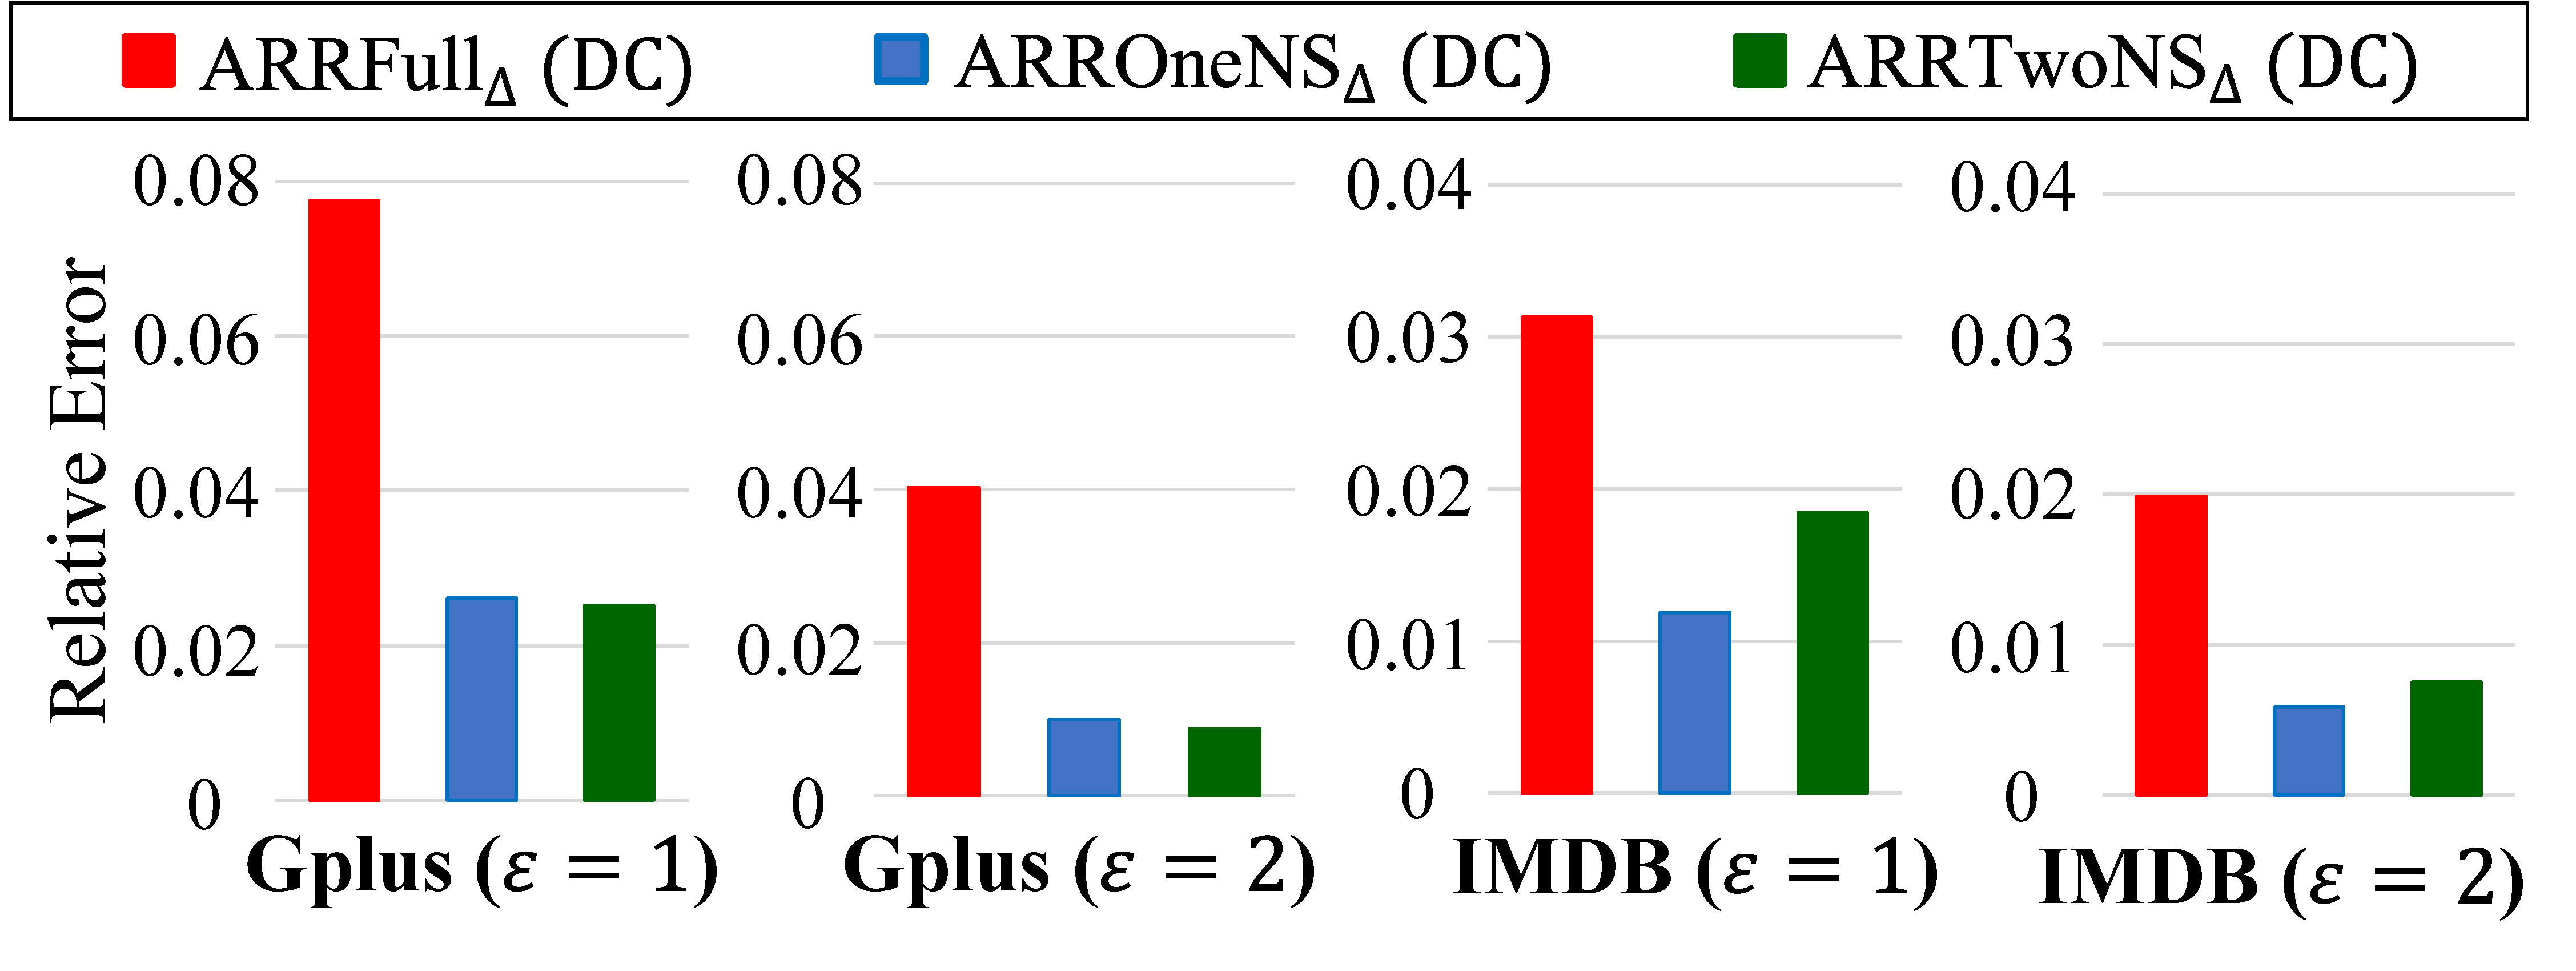
\includegraphics[width=0.96\linewidth]{fig/res2_w_Lap_abst2.pdf}
  \vspace{-6mm}
  \caption{Relative error of our three algorithms with double clipping (``DC'') when $\epsilon=1$ or $2$ and %$\mu_F=10^{-3}$ 
  $\mu^*=10^{-3}$ 
  ($n=107614$ in \GPlus{}, $n=896308$ in \IMDB{}).} 
  \label{chap2-fig:res2_w_Lap_abst}
%\end{figure}
 \vspace{1mm}
%\begin{figure}[t]
  \centering
  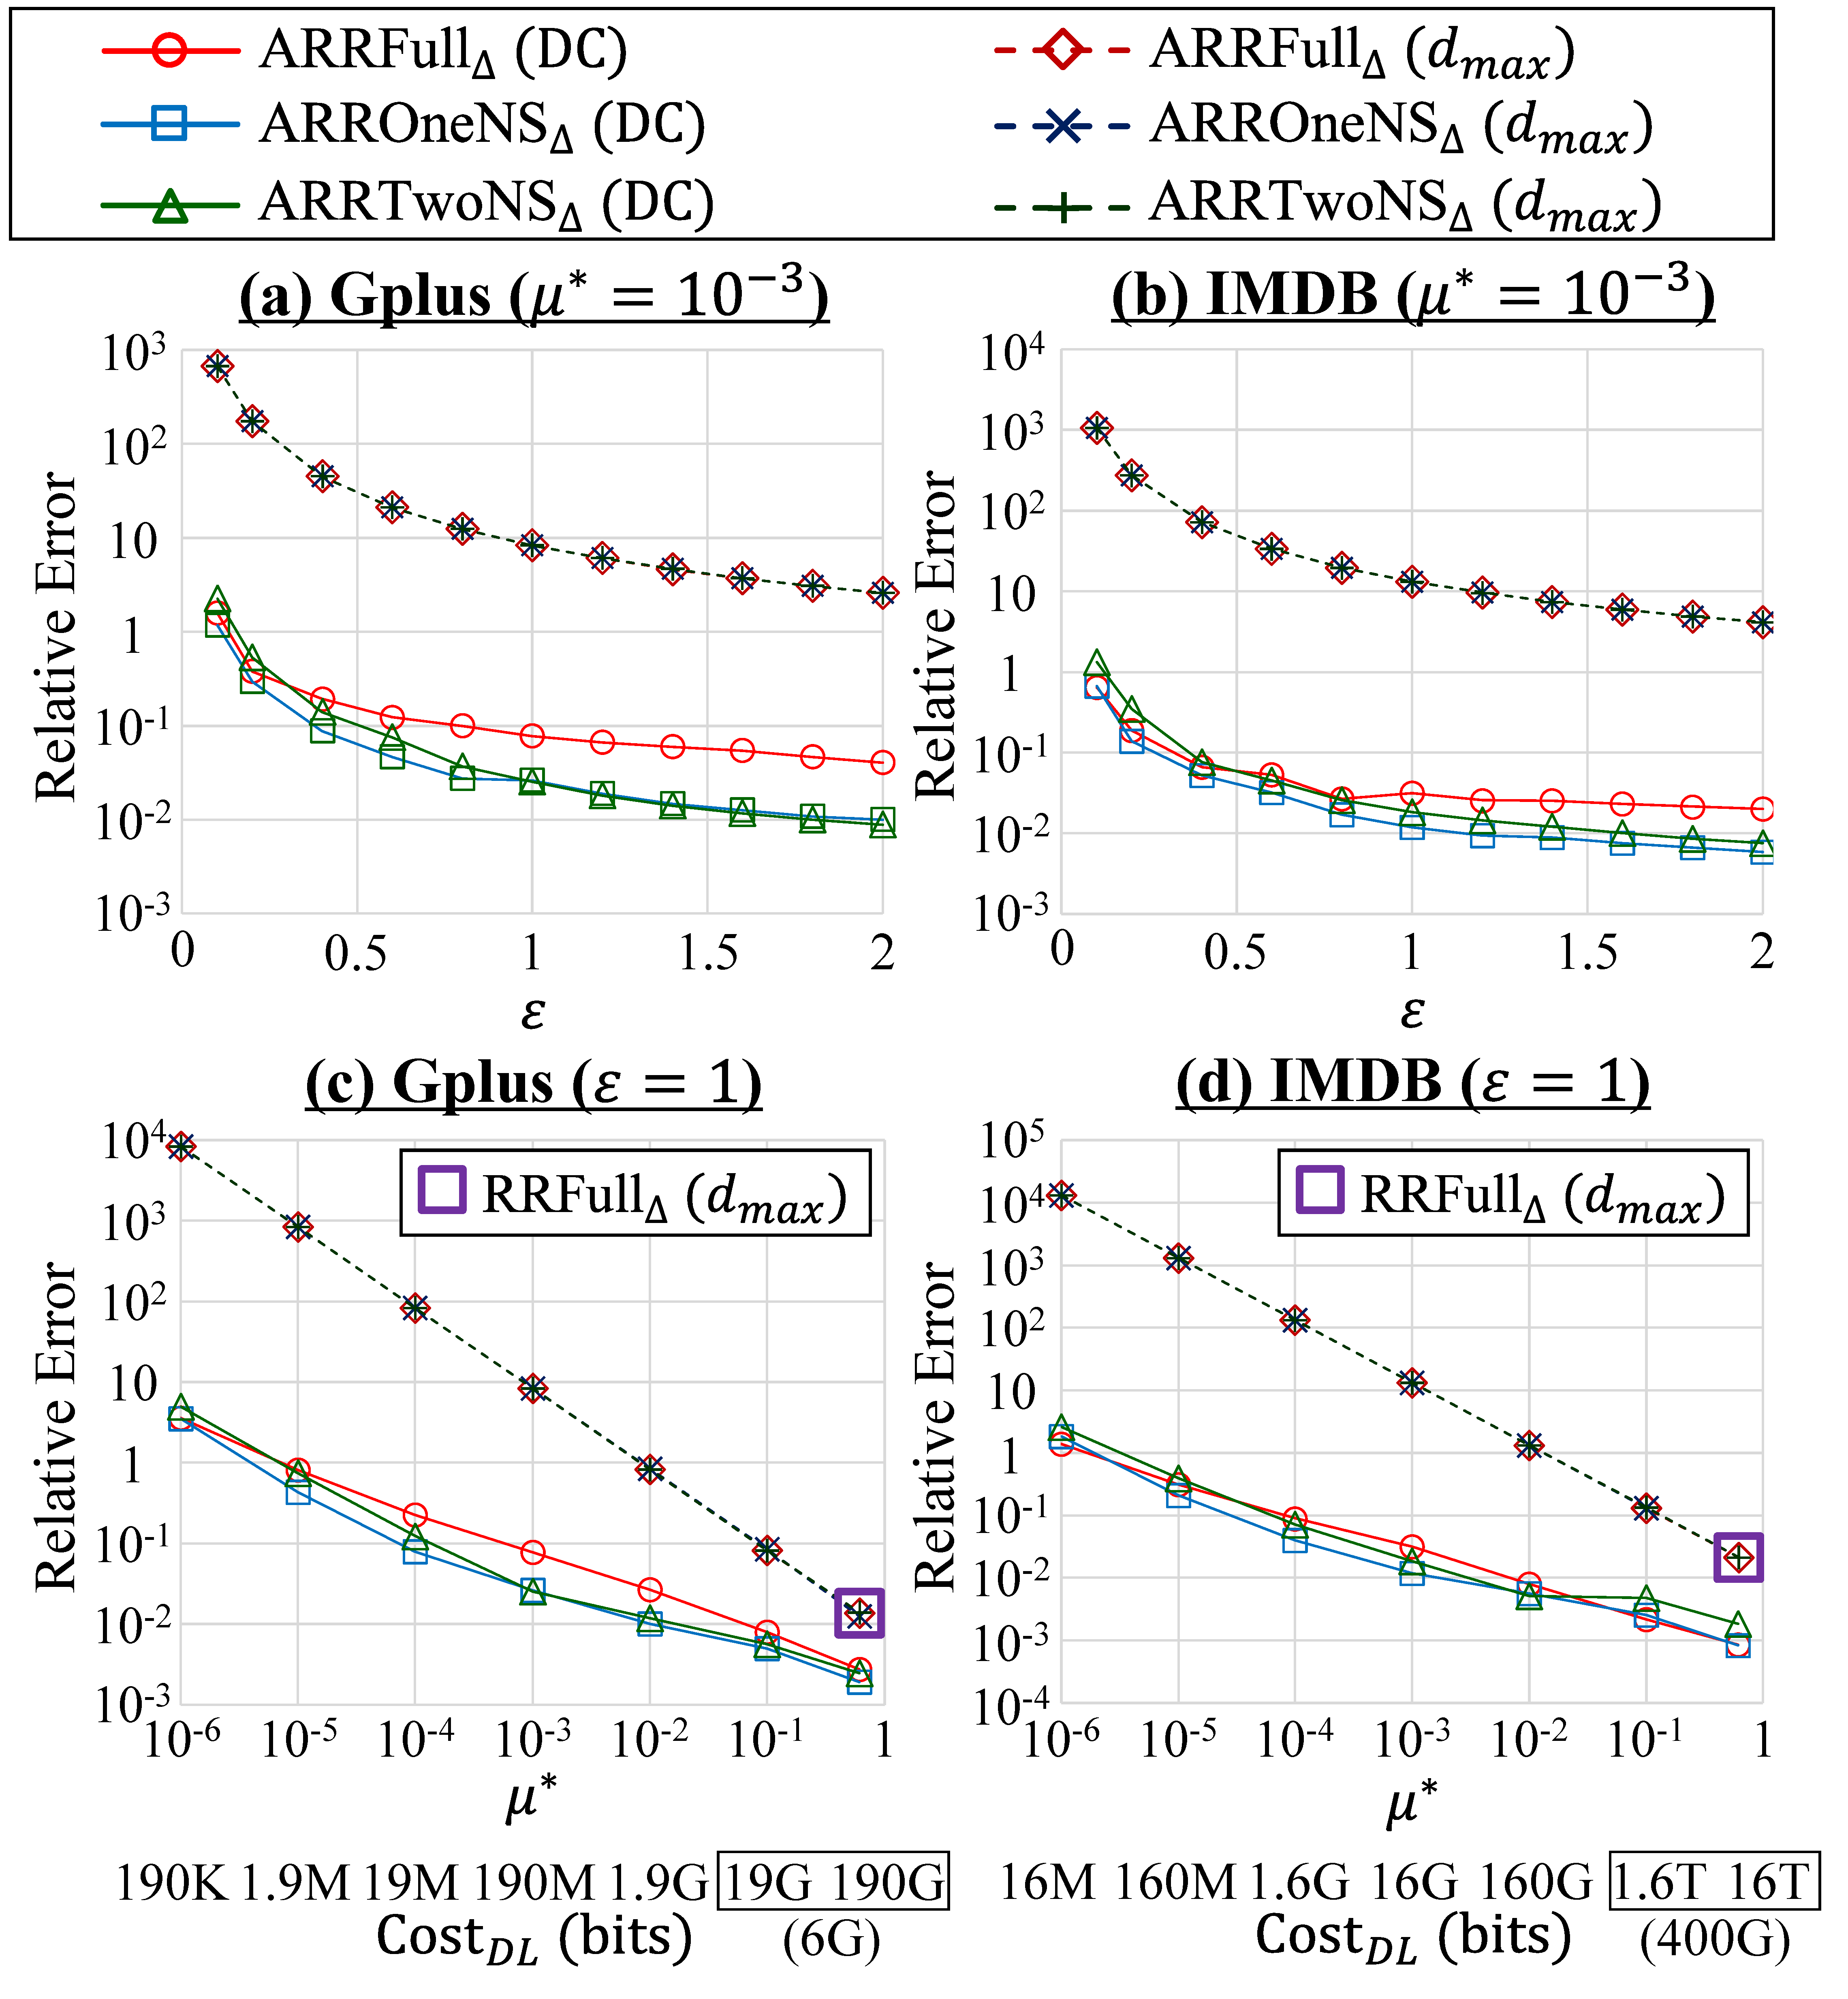
\includegraphics[width=0.99\linewidth]{fig/res2_w_Lap.pdf}
  \vspace{-5mm}
  \caption{Relative error of our three algorithms with (``DC'') or without (``$d_{max}$'') double clipping ($n=107614$ in \GPlus{}, $n=896308$ in \IMDB{}). \AlgSec{} is the 
  %two-rounds 
  algorithm in~\cite{Imola_USENIX21}. 
  $\CostDL$ is 
  %calculated by 
  an upper-bound in 
  (\ref{chap2-eq:CostDL_F}). 
  %Note that 
  When $\mu^* \geq 0.1$, 
  %(marked with squares), 
  $\CostDL$ can be $6$ Gbits and $400$ Gbits in \GPlus{} and \IMDB{}, respectively, by downloading only 0/1 for each pair of users $(v_j,v_k)$.} 
  \label{chap2-fig:res2_w_Lap}
\end{figure}

% \begin{table}[t]
% \caption{Basic notations.} 
% \centering
% \hbox to\hsize{\hfil
% \begin{tabular}{l|l|l}
% \hline
% Algorithm		&	\GPlus{} ($\epsilon=1$) &  \IMDB{}  ($\epsilon=1$)\\
% \hline
% \AlgOne{}   &   $0.078$   &   $0.031$\\
% \hline
% \end{tabular}
% \hfil}
% \label{chap2-tab:res2_w_Lap_abst}
% \end{table}

Figures~\ref{chap2-fig:res2_w_Lap_abst} and \ref{chap2-fig:res2_w_Lap} show the results. 
Figure~\ref{chap2-fig:res2_w_Lap_abst} highlights the relative error of our three algorithms with double clipping when $\epsilon=1$ or $2$ and $\mu^*=10^{-3}$. 
% Figure \ref{chap2-fig:res2_w_Lap} shows the results. 
``DC'' (resp.~``$d_{max}$'') represents algorithms with (resp.~without) double clipping. 
\AlgSec{} (marked with purple square) in Figure~\ref{chap2-fig:res2_w_Lap} (c) and (d) represents the two-rounds algorithm in~\cite{Imola_USENIX21}. 
Note that this is a special case of our \AlgOne{} without sampling ($\mu =\frac{e^{\epsilon_1}}{e^{\epsilon_1}+1} = 0.62$). 
% as described in Section~\ref{chap2-sub:algorithms_overview}. 
Figure~\ref{chap2-fig:res2_w_Lap} (c) and (d) also show the download cost $\CostDL$ calculated by 
(\ref{chap2-eq:CostDL_F}). 
Note that 
when $\mu^* \geq 0.1$ (marked with squares), 
$\CostDL$ can be $6$Gbits and $400$Gbits in \GPlus{} and \IMDB{}, respectively, by downloading only 0/1 for each pair of users $(v_j,v_k)$; $\CostDL = \frac{(n-1)(n-2)}{2}$ in this case. 
% $\CostDL$ is $400$Gbits and $6$Gbits in \GPlus{} and \IMDB{}, respectively, when user $v_i$ downloads only 0/1 for each 
% pair of users $(v_j,v_k)$ ($\CostDL = \frac{(n-1)(n-2)}{2}$ in this case). 

Figures~\ref{chap2-fig:res2_w_Lap_abst} and \ref{chap2-fig:res2_w_Lap} show that our \AlgTwo{} (DC) 
% with double clipping 
provides the best (or almost the best) performance in all cases. 
This is because \AlgTwo{} (DC) introduces the $4$-cycle trick 
% (shown in Figure~\ref{chap2-fig:four-cycle}) 
and effectively reduces the global sensitivity of the Laplacian noise by double clipping. 
% \AlgThree{} (DC) is outperformed by \AlgTwo{} (DC), 
% \AlgTwo{} (DC) outperforms \AlgThree{} (DC), 
% especially when $\epsilon$ or $\mu_F$ ($=\mu_O^2 = \mu_T^3$) is small 
% (e.g., $\epsilon=0.1$ to $0.8$, $\mu_F=10^{-6}$ to $10^{-4}$). 
% There are two reasons for this: 
% (1) \AlgThree{} cannot effectively reduce the global sensitivity by double clipping,
% (2) the Laplacian noise increases with decrease in $\epsilon$ or $\mu_F$, 
% This is because \AlgThree{} cannot effectively reduce the global sensitivity by double clipping and the Laplacian noise increases with decrease in $\epsilon$ or $\mu_F$ 
% and has a non-negligible effect on the estimation error for small $\epsilon$ or $\mu_F$, 
% (as shown in Table~\ref{chap2-tab:privacy_utility_cost} of Section~\ref{chap2-sub:clip_theoretical_analysis}). 
% The difference between \AlgTwo{} (DC) and \AlgOne{} (DC) is also small for very small $\epsilon$ or $\mu_F$ (e.g., $\epsilon=0.1$, $\mu_F=10^{-6}$) because the Laplacian noise is dominant in this case. 
% Later, we will also 
% provide a detailed investigation of the relation between the Laplacian noise and the relative error while changing $n$. 
% to answer our research question RQ1. 
Later, we will 
% also 
% provide a detailed investigation of 
investigate 
the effectiveness of the $4$-cycle trick in detail 
by not adding the Laplacian noise. 
% and 
We will also investigate 
%the relation between the Laplacian noise and the relative error 
the impact of the Laplacian noise 
while changing $n$. 

Figure~\ref{chap2-fig:res2_w_Lap} also shows that 
the relative error is almost the same between our three algorithms without double clipping (``$d_{max}$'') and that it is too large. 
% the relative error of our three algorithms without double clipping is too large and that it is almost the same between the three. 
This is because $\Lap(\frac{d_{max}}{\epsilon_2}$) is too large and dominant. 
The relative error is significantly reduced by introducing our double clipping in all cases. 
% For example, our \AlgTwo{} (DC) without sampling ($\mu_F =\frac{e^{\epsilon_1}}{e^{\epsilon_1}+1}$)
For example, when $\mu^* = 10^{-3}$, our double clipping reduces the relative error of \AlgTwo{} by two or three orders of magnitude. 
% \AlgTwo{} (DC) also reduces the expected download size by $\mu_F = \mu_O^2 = 10^{-3}$ while keeping roughly the same relative error as the algorithm in~\cite{Imola_USENIX21}, thanks to double clipping. 
The improvement is larger for smaller $\mu^*$. 

In \conference{the full version \cite{Imola_arXiv22}}\arxiv{Appendix~\ref{chap2-sec:EC_DC}}, we also evaluate the effect of edge clipping and noisy triangle clipping independently and show that each component significantly reduces the relative error. 

\smallskip
\noindent{\textbf{Communication Cost.}}~~From Figure~\ref{chap2-fig:res2_w_Lap} (c) and (d), we can explain how much our algorithms can reduce the download cost while keeping high utility, e.g., relative error $\ll 1$. 

For example, when we use the algorithm in \cite{Imola_USENIX21}, the download cost is 
$\CostDL = 400$ Gbits in \IMDB{}. 
% $\CostDL = 400$ Gbits and $6$ Gbits in \GPlus{} and \IMDB{}, respectively. 
Thus, when the download speed is $20$ Mbps 
% (which is a 
(recommended speed in YouTube \cite{YouTube_speed}), every user $v_i$ needs 6 hours to download the message $M_i$, which is far from practical. 
In contrast, our \AlgTwo{} (DC) can reduce it to 
% $100$ 
$160$ 
Mbits (8 seconds when $20$ Mbps download rate) or less 
while keeping relative error $= 0.21$, 
% (relative error $= 0.21$), 
% or $1$ Gbits (relative error $= 0.040$). 
% Consequently, every user needs only 
% 5 
% 8 
% or 50 
% seconds or less, 
which is practical and a dramatic improvement over \cite{Imola_USENIX21}. 
% Therefore, private triangle counting is now practical.

We also note that since $d_{max} \ll n$ in \IMDB{}, 
% the ARR outputs ``1'' with probability $\mu e^{-\epsilon_1}$ in most cases
% the download cost 
$\CostDL$ of our \AlgTwo{} (DC) 
can also be roughly approximated by $60$ Mbits (3 seconds) by replacing $\mu$ with $\mu e^{-\epsilon_1}$ in 
(\ref{chap2-eq:CostDL_F}). 
%(\ref{chap2-eq:CostDL_O}). 

% We also note that the upload cost is much smaller; e.g., by (\ref{chap2-eq:CostUL_proposal}), $\CostUL{} = 11$ Mbits in \IMDB{} even when $\mu=1$. 
% Thus, it is not an issue.

\smallskip
% \noindent{\textbf{Three Algorithms w/o Lap.}}~~
\noindent{\textbf{4-Cycle Trick.}}~~We 
% first evaluated 
also investigated 
% how well our two algorithms \AlgTwo{} and \AlgThree{} address the $4$-cycle issue of \AlgOne{} 
the effectiveness of our $4$-cycle trick in \AlgTwo{} and \AlgThree{} 
% (shown in Figure~\ref{chap2-fig:four-cycle}) 
in detail. 
% explained in Section~\ref{chap2-sub:algorithms_overview}. 
% the relation between the $4$-cycle issue 
To this end, we evaluated our three algorithms when we did \textit{not} add the Laplacian noise at the second round. 
% (i.e., $\epsilon_2 = \infty$). 
Note that they do not provide edge LDP, as $\epsilon_2 = \infty$. 
The purpose here is to purely investigate the effectiveness of the $4$-cycle trick 
% issue 
related to our first research question RQ1. 
% We will report experimental results of the three algorithms with the Laplacian noise later. 

\begin{figure}[t]
  \centering
  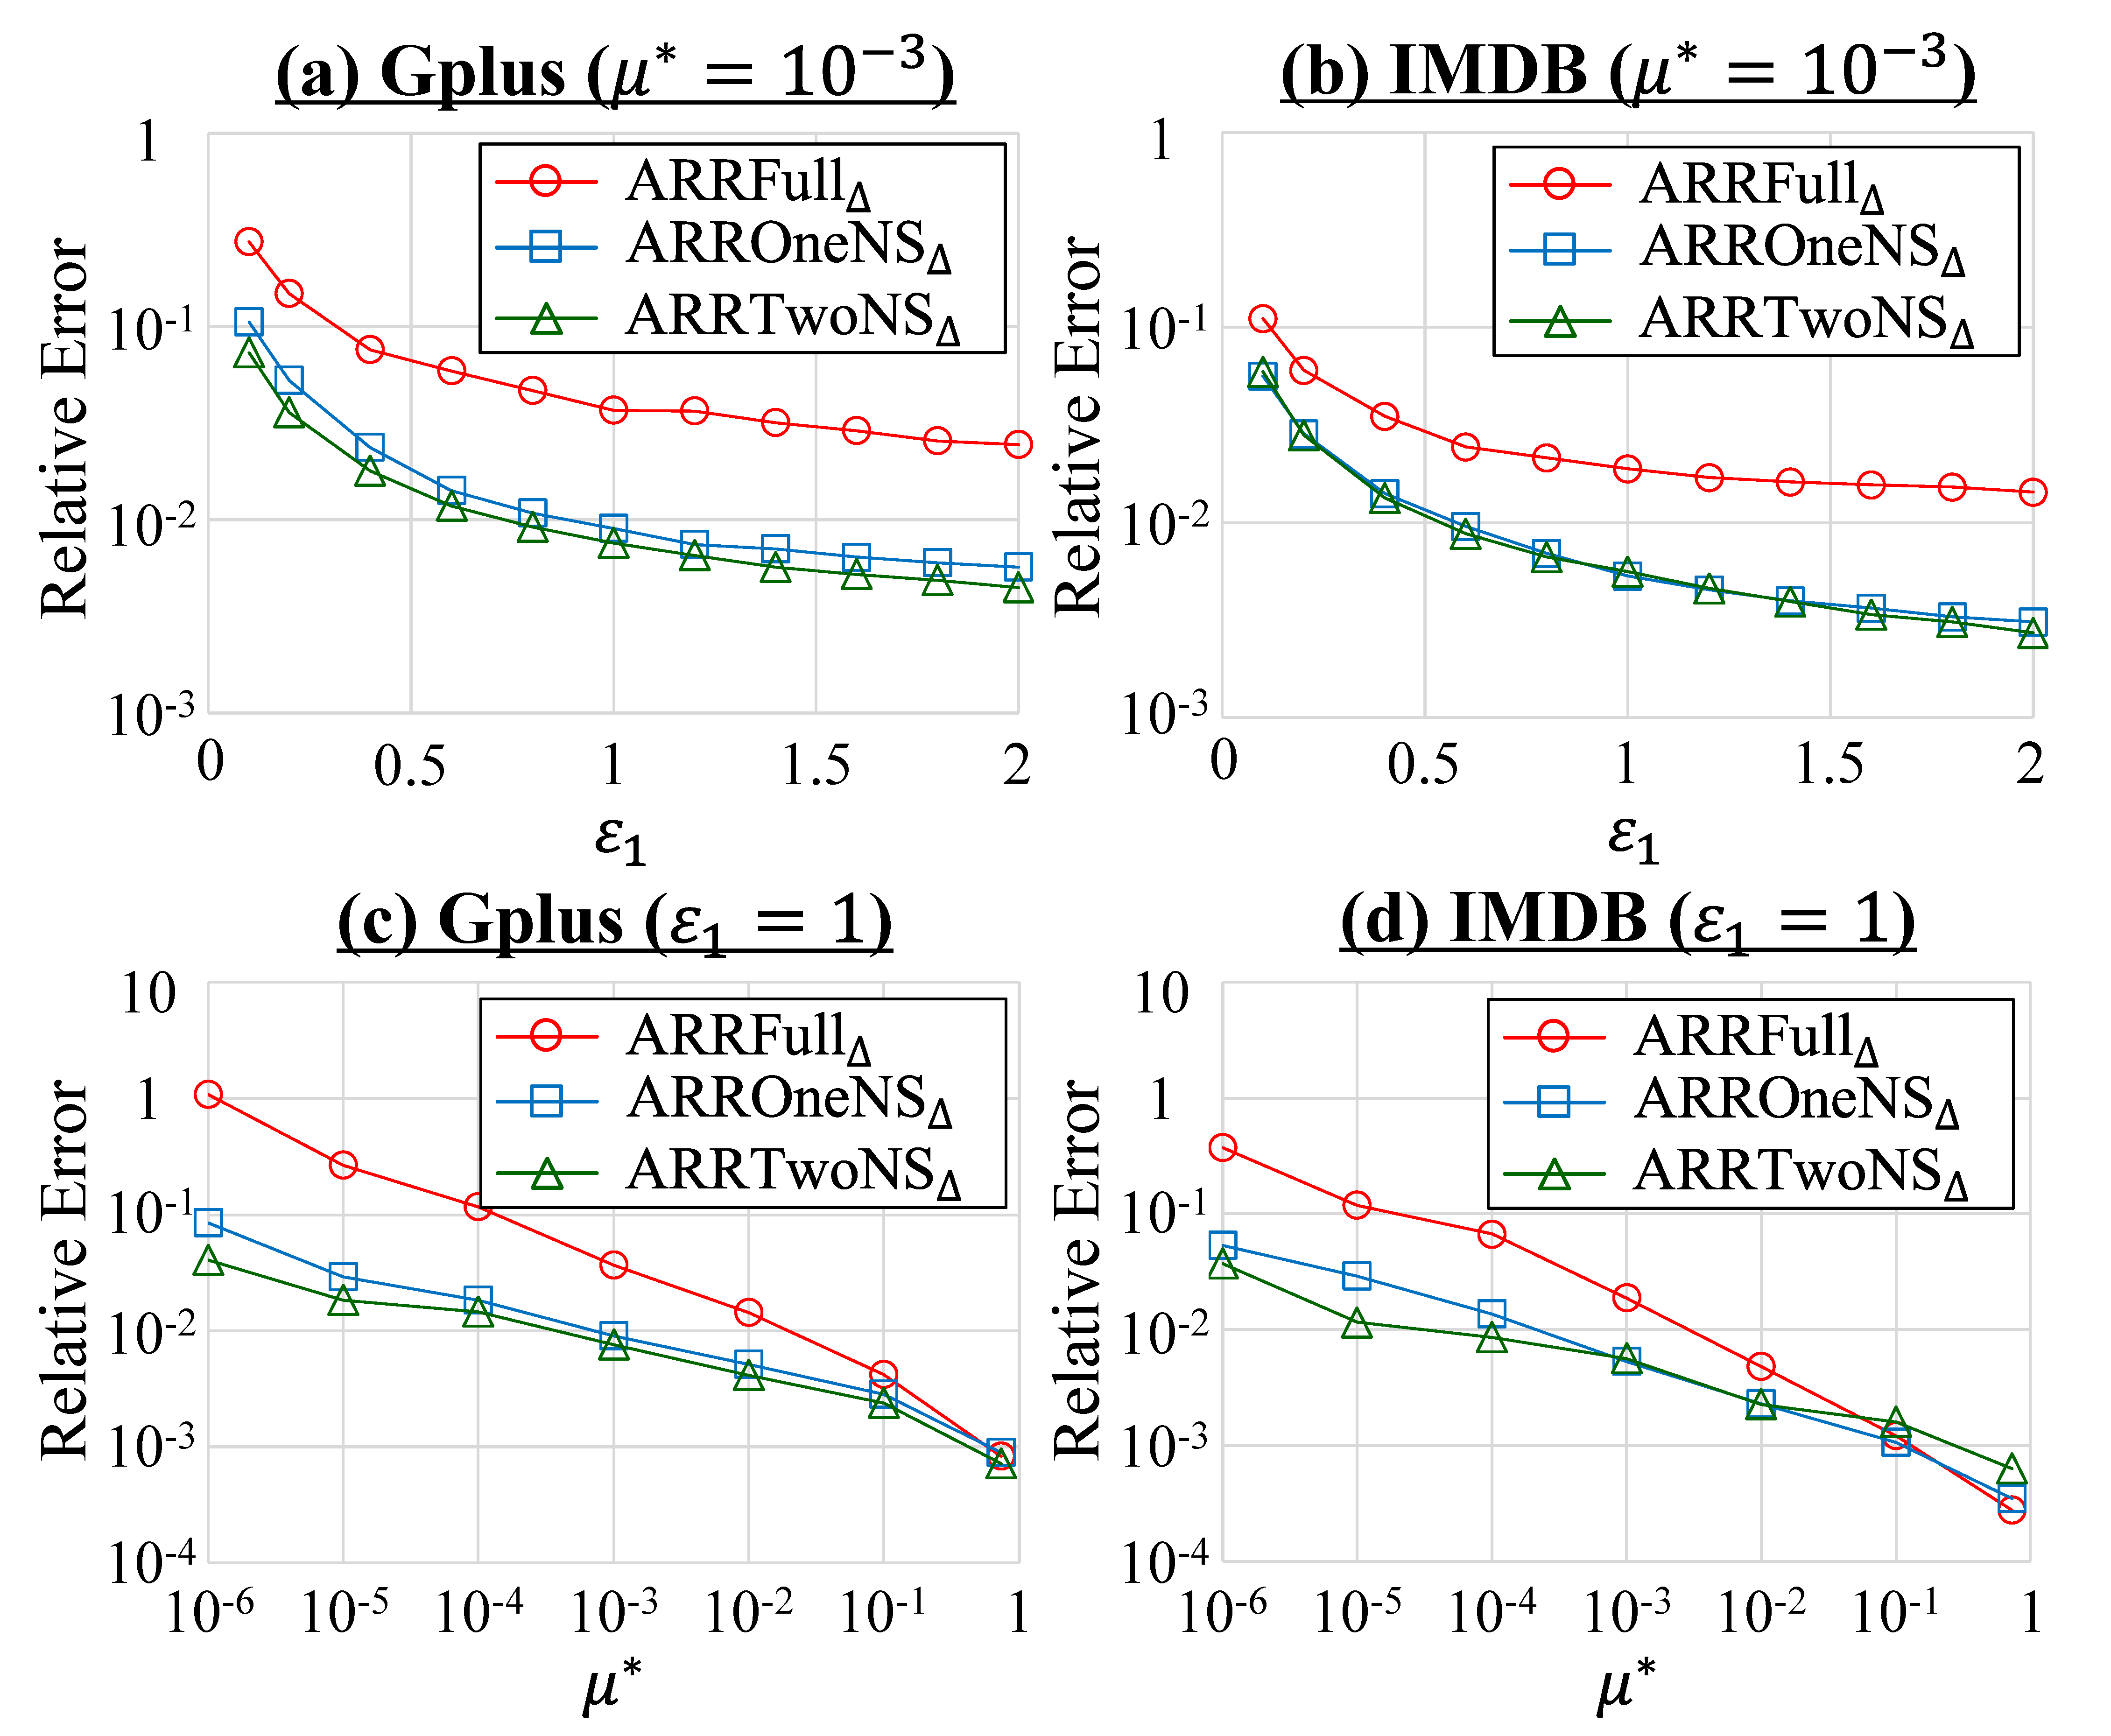
\includegraphics[width=0.99\linewidth]{fig/res1_wo_Lap.pdf}
  \vspace{-5mm}
  \caption{Relative error of our three algorithms without the Laplacian noise 
  % at the second round 
  ($n=107614$ in \GPlus{}, $n=896308$ in \IMDB{}).} 
  \label{chap2-fig:res1_wo_Lap}
\end{figure}

% We first evaluated our three triangle counting algorithms with double clipping. 
Figure~\ref{chap2-fig:res1_wo_Lap} shows the results, where 
% $\mu_F$ (resp.~$\epsilon_1$) is changed from $10^{-6}$ to $1$ (resp.~$0.1$ to $2$). 
% $\epsilon_1$ (resp.~$\mu_F$) is changed from $0.1$ to $2$ (resp.~$10^{-6}$ to $\frac{e^{\mu_F}}{e^{\mu_F} + 1}$). 
$\epsilon_1$ and 
% $\mu_F$ ($= \mu_O^2 = \mu_T^3$) 
$\mu^*$ 
are changed to various values. 
Figure~\ref{chap2-fig:res1_wo_Lap} shows that \AlgTwo{} and \AlgThree{} significantly outperform \AlgOne{} when 
% $\mu_F$ 
$\mu^*$ 
is small. 
This is because in both \AlgTwo{} and \AlgThree{}, 
% the first term in the expected $l_2$ loss 
the factors of 
% $S_3$ (\#3-stars) and $P_3$ (\#3-paths) 
$C_4$ (\#4-cycles) and $S_3$ (\#3-stars) 
in the expected $l_2$ loss 
diminish 
for small $\mu$, 
% as 
% $\mu_F$ ($= \mu_O^2 = \mu_T^3$) 
% the parameter $\mu$ in the ARR 
% goes to $0$, 
as explained in Section~\ref{chap2-sub:algorithms_theoretical_analysis}. 
In other words, \AlgTwo{} and \AlgThree{} effectively address the $4$-cycle issue. 
Figure~\ref{chap2-fig:res1_wo_Lap} also shows that \AlgThree{} slightly outperforms \AlgTwo{} when $\mu^*$ is small. 
% (e.g., $10^{-6}$ to $10^{-4}$). 
This is because 
% the first term in the expected $l_2$ loss diminishes 
% the factors of $S_3$ and $P_3$ 
the factors of $C_4$ and $S_3$ 
diminish 
more rapidly; i.e., \AlgThree{} addresses the $4$-cycle issue more aggressively. 

However, when we add the Laplacian noise, \AlgThree{} (DC) is outperformed by \AlgTwo{} (DC), as shown in Figure~\ref{chap2-fig:res2_w_Lap}. 
% \AlgTwo{} (DC) outperforms \AlgThree{} (DC), 
% especially when $\epsilon$ or $\mu_F$ ($=\mu_O^2 = \mu_T^3$) is small 
% (e.g., $\epsilon=0.1$ to $0.8$, $\mu_F=10^{-6}$ to $10^{-4}$). 
This is because \AlgThree{} cannot effectively reduce the global sensitivity by double clipping. 
In Figure~\ref{chap2-fig:res2_w_Lap}, the difference between \AlgTwo{} (DC) and \AlgOne{} (DC) is also small for very small $\epsilon$ or $\mu^*$ (e.g., $\epsilon=0.1$, $\mu^*=10^{-6}$) because the Laplacian noise is dominant in this case. 
% (as shown in Table~\ref{chap2-tab:privacy_utility_cost} of Section~\ref{chap2-sub:clip_theoretical_analysis}). 

\smallskip
\noindent{\textbf{Changing $\bm{n}$.}}~~We 
finally 
% also 
evaluated our three algorithms with double clipping while changing the number $n$ of users. 
In both \GPlus{} and \IMDB{}, we randomly selected $n$ users from all users and extracted a graph with $n$ users. 
Then we evaluated the relative error while changing $n$ to various values.

\begin{figure}[t]
  \centering
  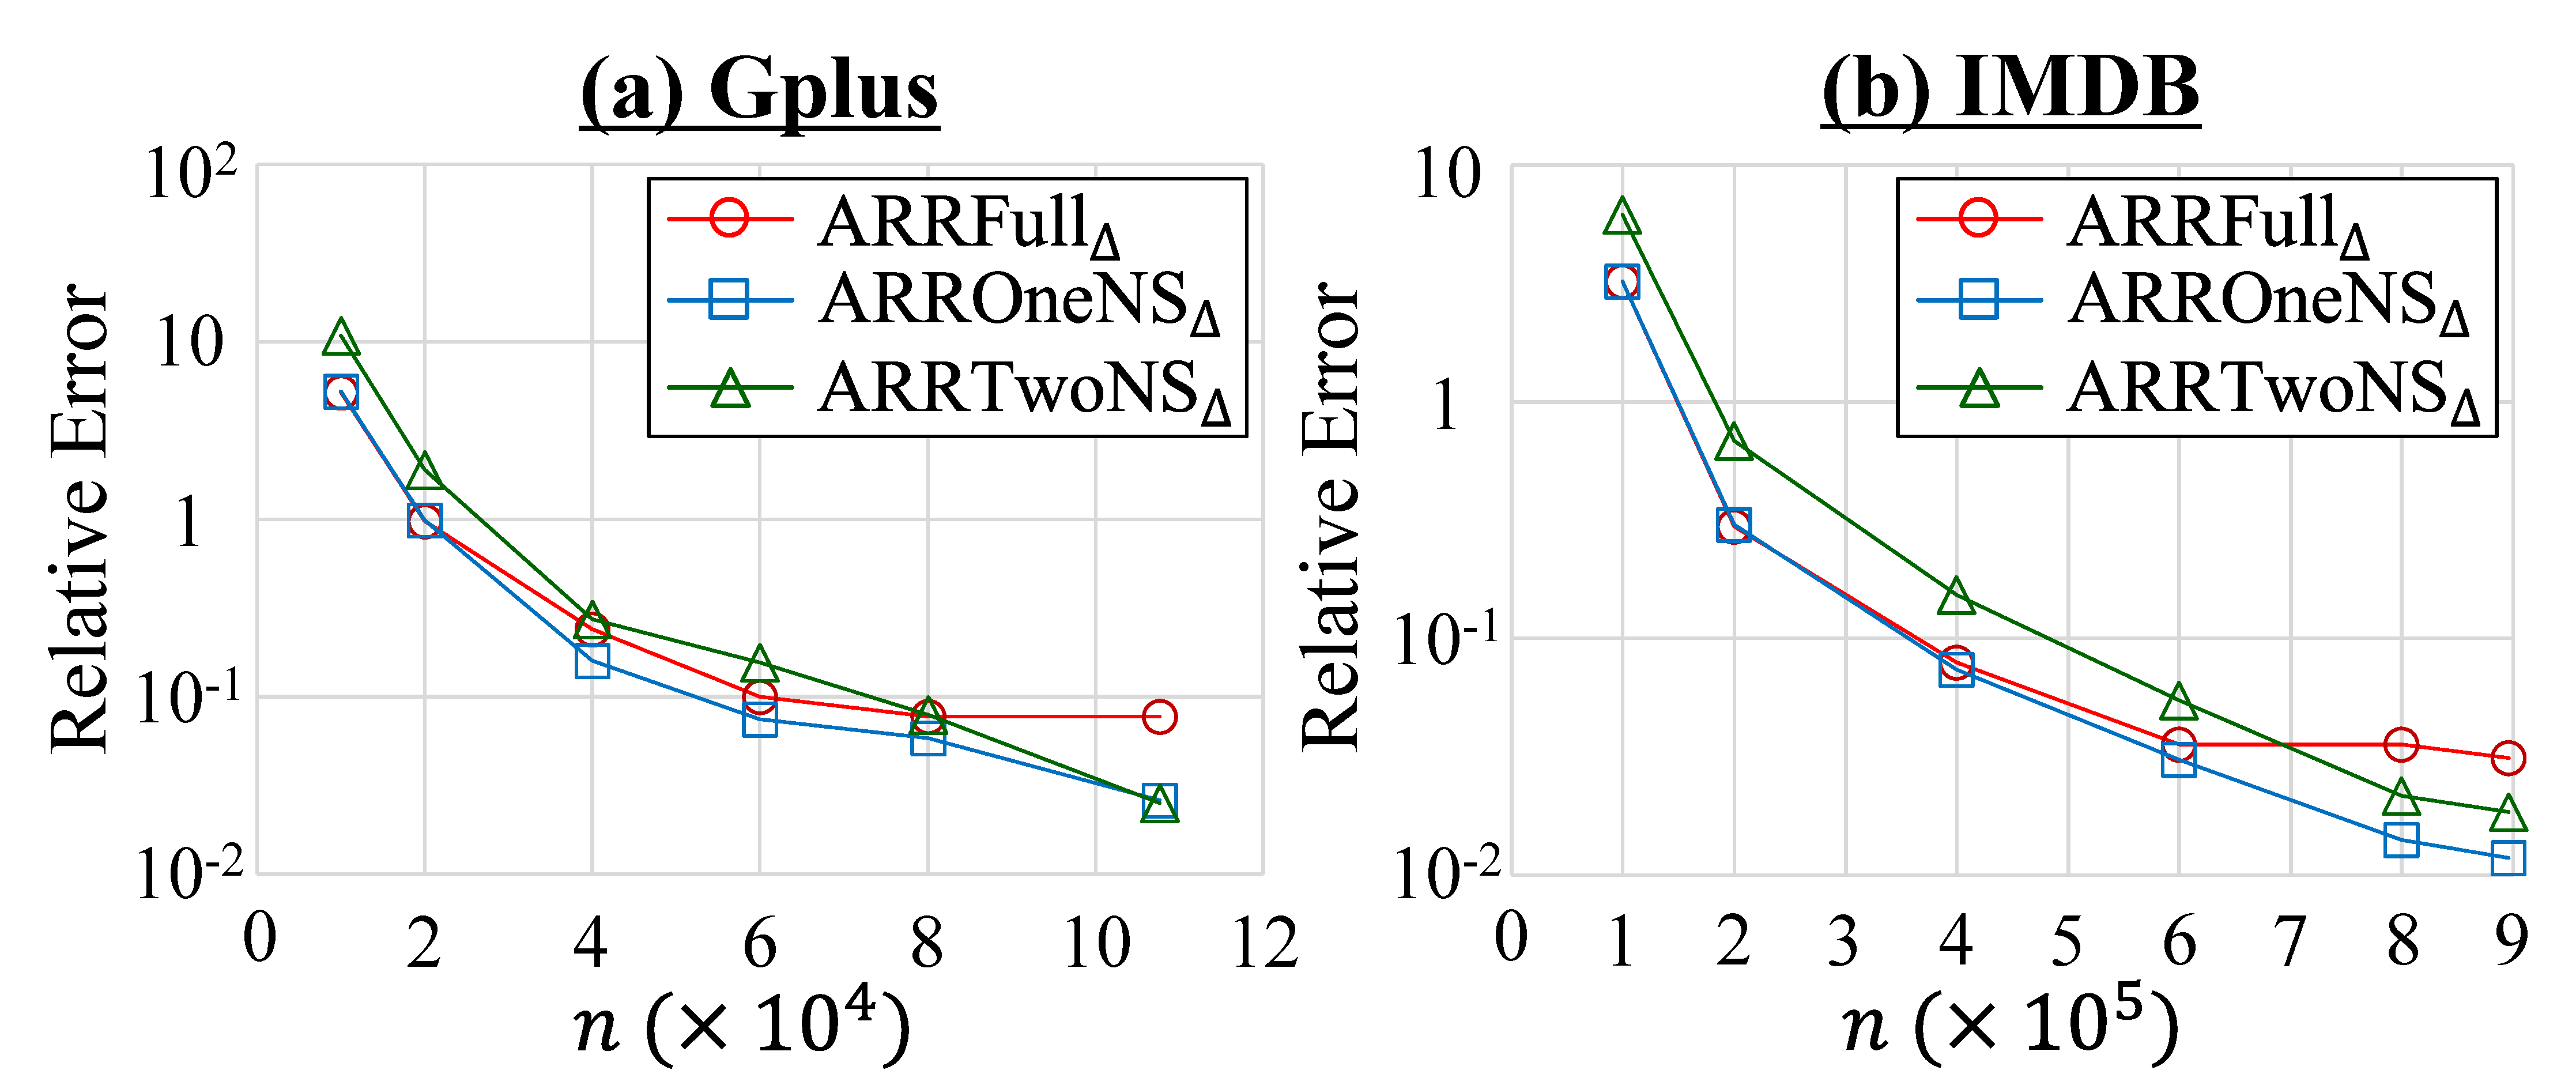
\includegraphics[width=0.99\linewidth]{fig/res3_n.pdf}
  \vspace{-4mm}
  \caption{Relative error of our three algorithms with double clipping for various values of $n$ 
  ($\epsilon=1$, $\mu^*=10^{-3}$).} 
  \label{chap2-fig:res3_n}
\end{figure}

Figure~\ref{chap2-fig:res3_n} shows the results, where $\epsilon=1$ ($\epsilon_0=0.1$, $\epsilon_1 = \epsilon_2 = 0.45$) and $\mu^* = 10^{-3}$. 
In all 
% the 
three algorithms, the relative error decreases with increase in $n$.
This is because the expected $l_2$ loss can be expressed as 
% $O(n)$ (when we regard $\epsilon$ and $\mu_F$ as constants and ignore $d_{max}$) 
$O(n d_{max}^3)$ or $O(n d_{max}^2)$ 
% (when we regard $\epsilon$ as constants) 
in these algorithms as shown in Section~\ref{chap2-sub:clip_theoretical_analysis} and the square of the true triangle count can be expressed as $\Omega(n^2)$.
In other words, when $d_{max} \ll n$, the relative error becomes smaller for larger $n$. 
% In other words, this is consistent with our theoretical results. 
Figure~\ref{chap2-fig:res3_n} also shows that for small $n$, \AlgThree{} provides the worst performance and 
\AlgTwo{} performs almost the same as \AlgOne{}. 
% the difference between \AlgTwo{} and \AlgOne{} is very small. 
For large $n$, 
% \AlgThree{} outperforms \AlgOne{} and 
\AlgOne{} performs the worst and 
\AlgTwo{} performs the best. 


To investigate the reason for this, we decomposed the estimation error into two components -- 
the first error caused by empirical estimation and the second error caused by the Laplacian noise. 
Specifically, for each algorithm, 
we evaluated the first error by calculating the relative error when we did not add the Laplacian noise ($\epsilon_1 = 0.45$). 
Then we evaluated the second error by subtracting the first error from the relative error when we used double clipping ($\epsilon_0=0.1$, $\epsilon_1 = \epsilon_2 = 0.45$). 

Figure~\ref{chap2-fig:res3_emp_Lap} shows the results for some values of $n$, where ``emp'' represents the first error by empirical estimation and ``Lap'' represents the second error by the Laplacian noise. 
We observe that the second error 
rapidly decreases with increase in $n$. 
% The difference between \AlgOne{} and \AlgTwo{} 
% This is because the expected $l_2$ loss of the Laplacian noise is $O(\sum_{i=1}^n \kappa_i^2)$, 
% which is much smaller than $O(n d_{max}^2)$, 
% as shown in Section~\ref{chap2-sub:clip_theoretical_analysis}. 
In addition, 
% Figure~\ref{chap2-fig:res3_emp_Lap} also shows that 
the first error of \AlgOne{} is much larger than those of \AlgTwo{} and \AlgThree{} when $n$ is large. 

We also examined 
% the maximum degree $d_{max}$ and 
the number $C_4$ of $4$-cycles as a function of $n$. Figure~\ref{chap2-fig:res4_4cycles} shows the results. 
We observe that $C_4$ (which is $O(n d_{max}^3)$) is quartic in $n$; e.g., $C_4$ is increased by $2^4 \approx 10$ and $6^4 \approx 10^3$ when $n$ is multiplied by $2$ and $6$, respectively. 
This is because we randomly selected $n$ users from all users and $d_{max}$ is almost proportional to $n$ (though $d_{max} \ll n$). 
% We observe that $d_{max}$ is proportional to $n$ (though $d_{max} \ll n$). 
% This is because we randomly selected $n$ users from all users. 
% Consequently, $C_4$ which can be expressed as $O(n d_{max}^3)$ is quartic in $n$; e.g., $C_4$ is increased by $2^4 \approx 10$ and $6^4 \approx 10^3$ when $n$ is multiplied by $2$ and $6$, respectively. 

\begin{figure}[t]
  \centering
  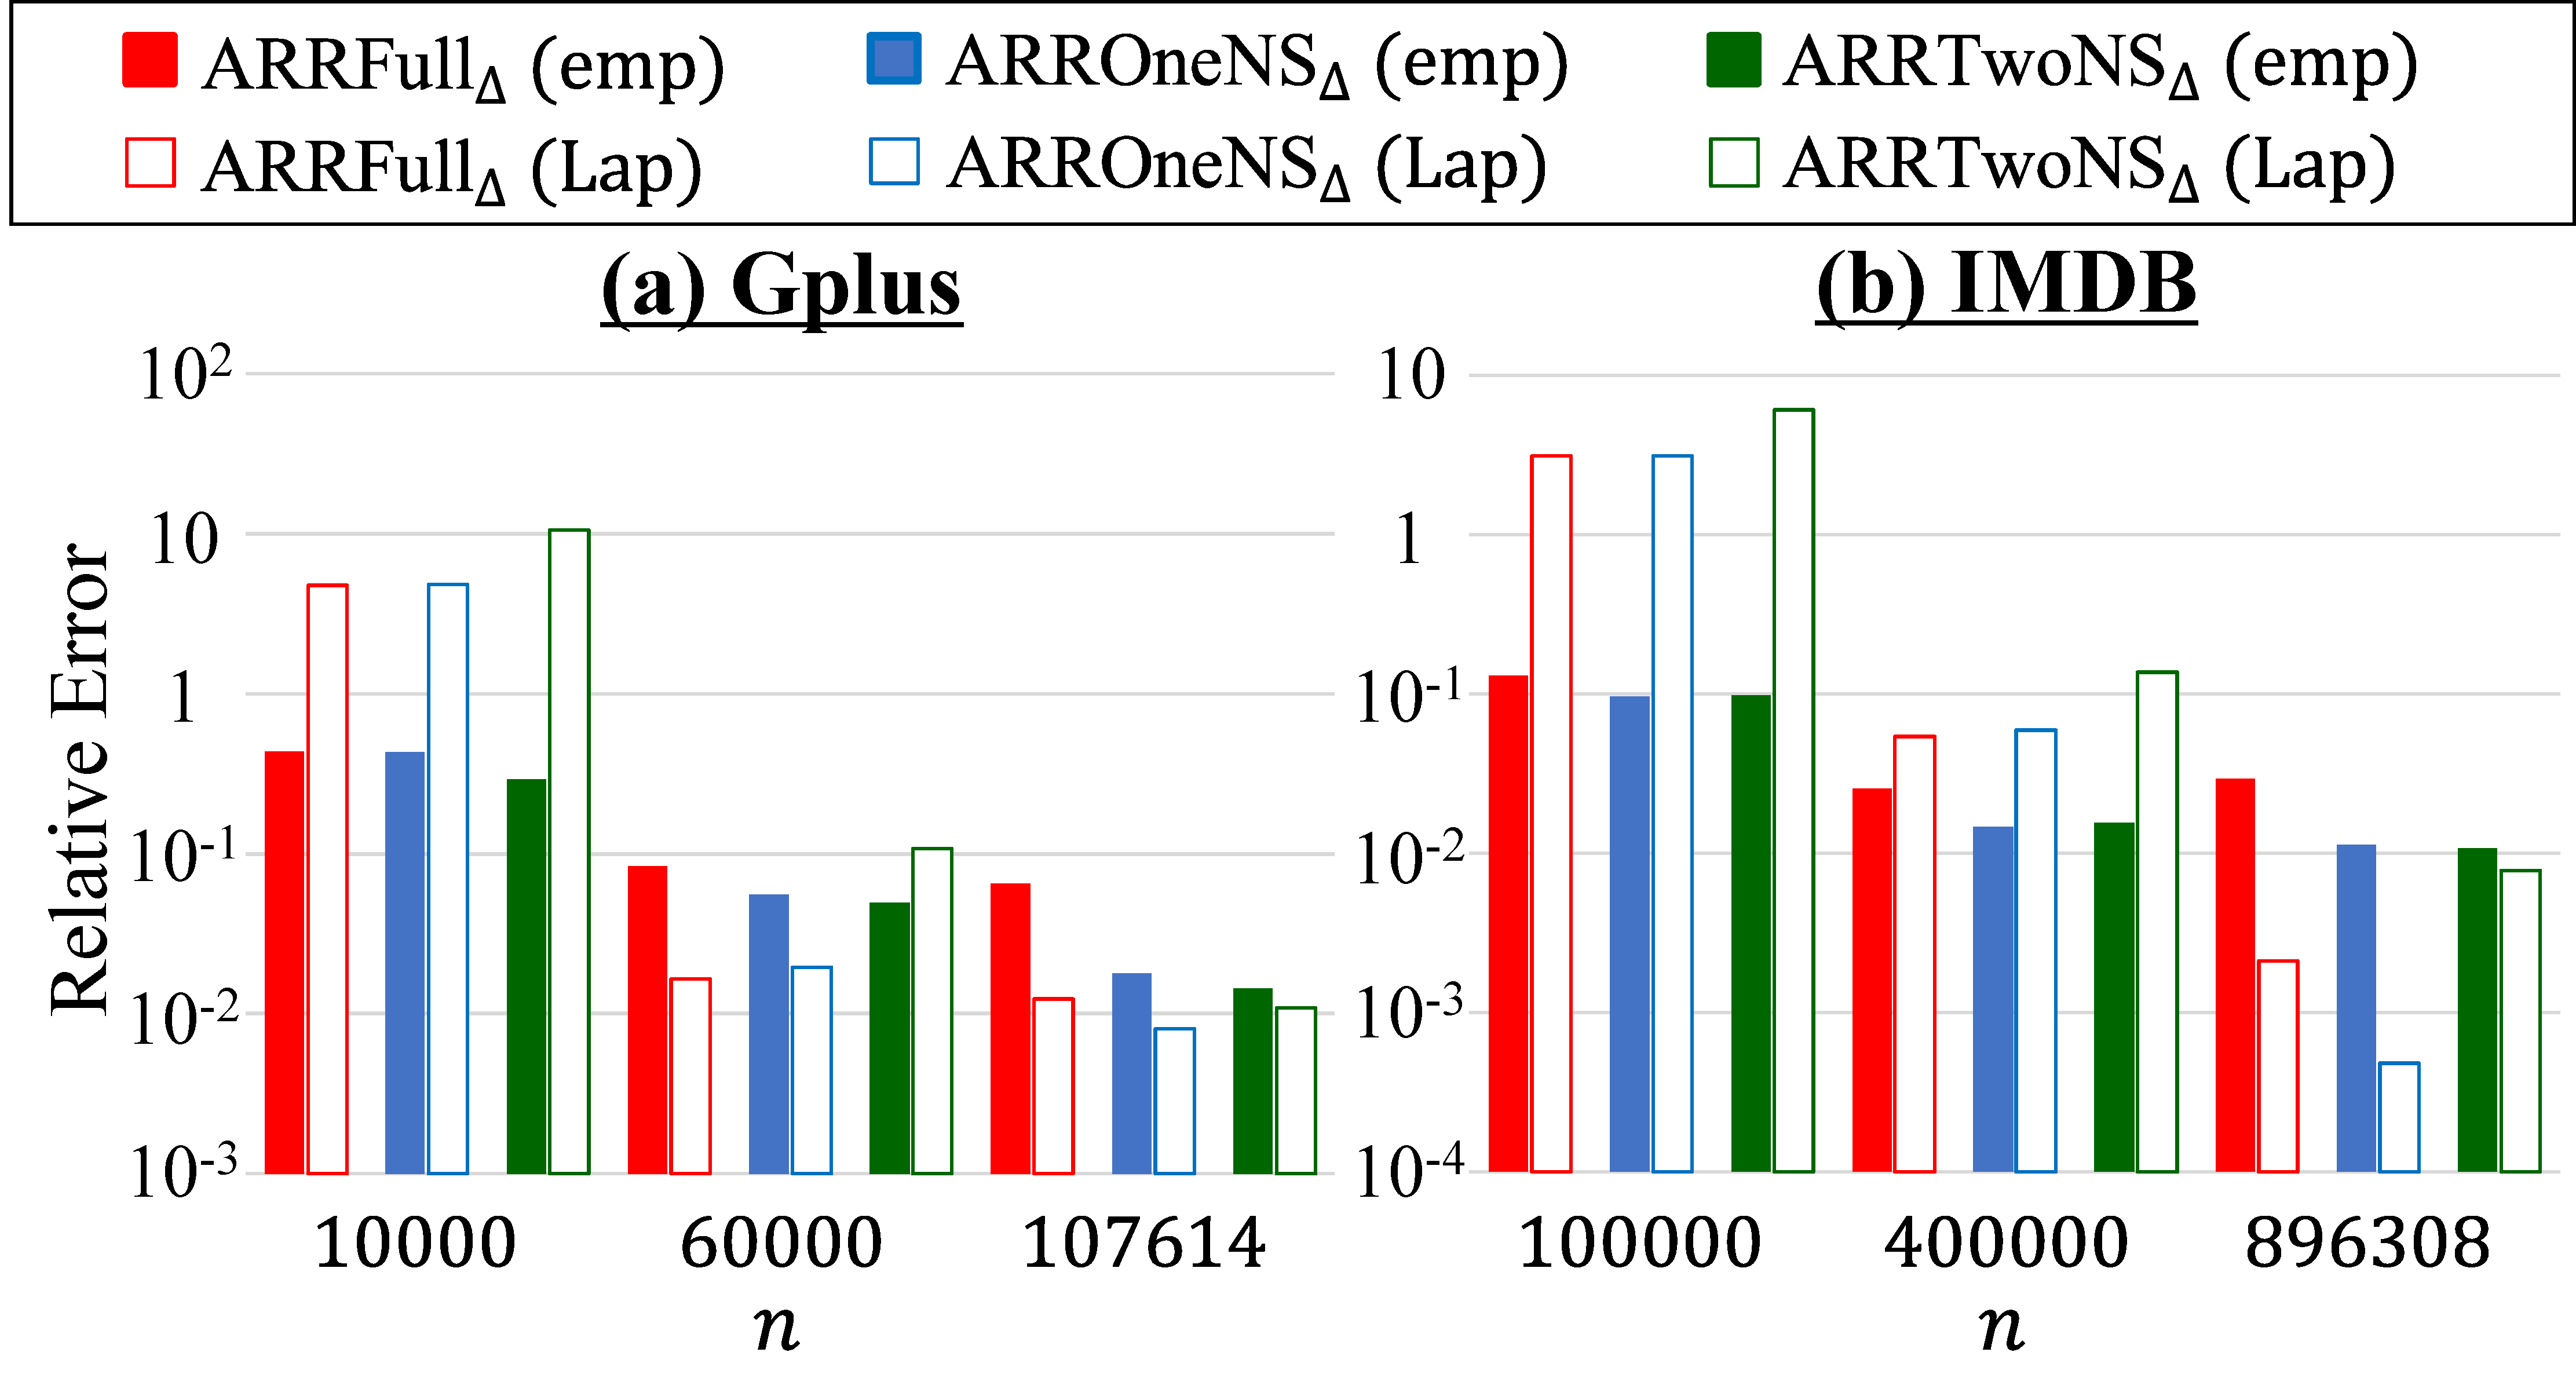
\includegraphics[width=0.99\linewidth]{fig/res3_emp_Lap.pdf}
  \vspace{-5mm}
  \caption{Relative error of empirical estimation and the Laplacian noise in our three algorithms with double clipping ($\epsilon=1$, $\mu^*=10^{-3}$).} 
  \label{chap2-fig:res3_emp_Lap}
% \end{figure}
 \vspace{1mm}
% \begin{figure}[t]
  \centering
  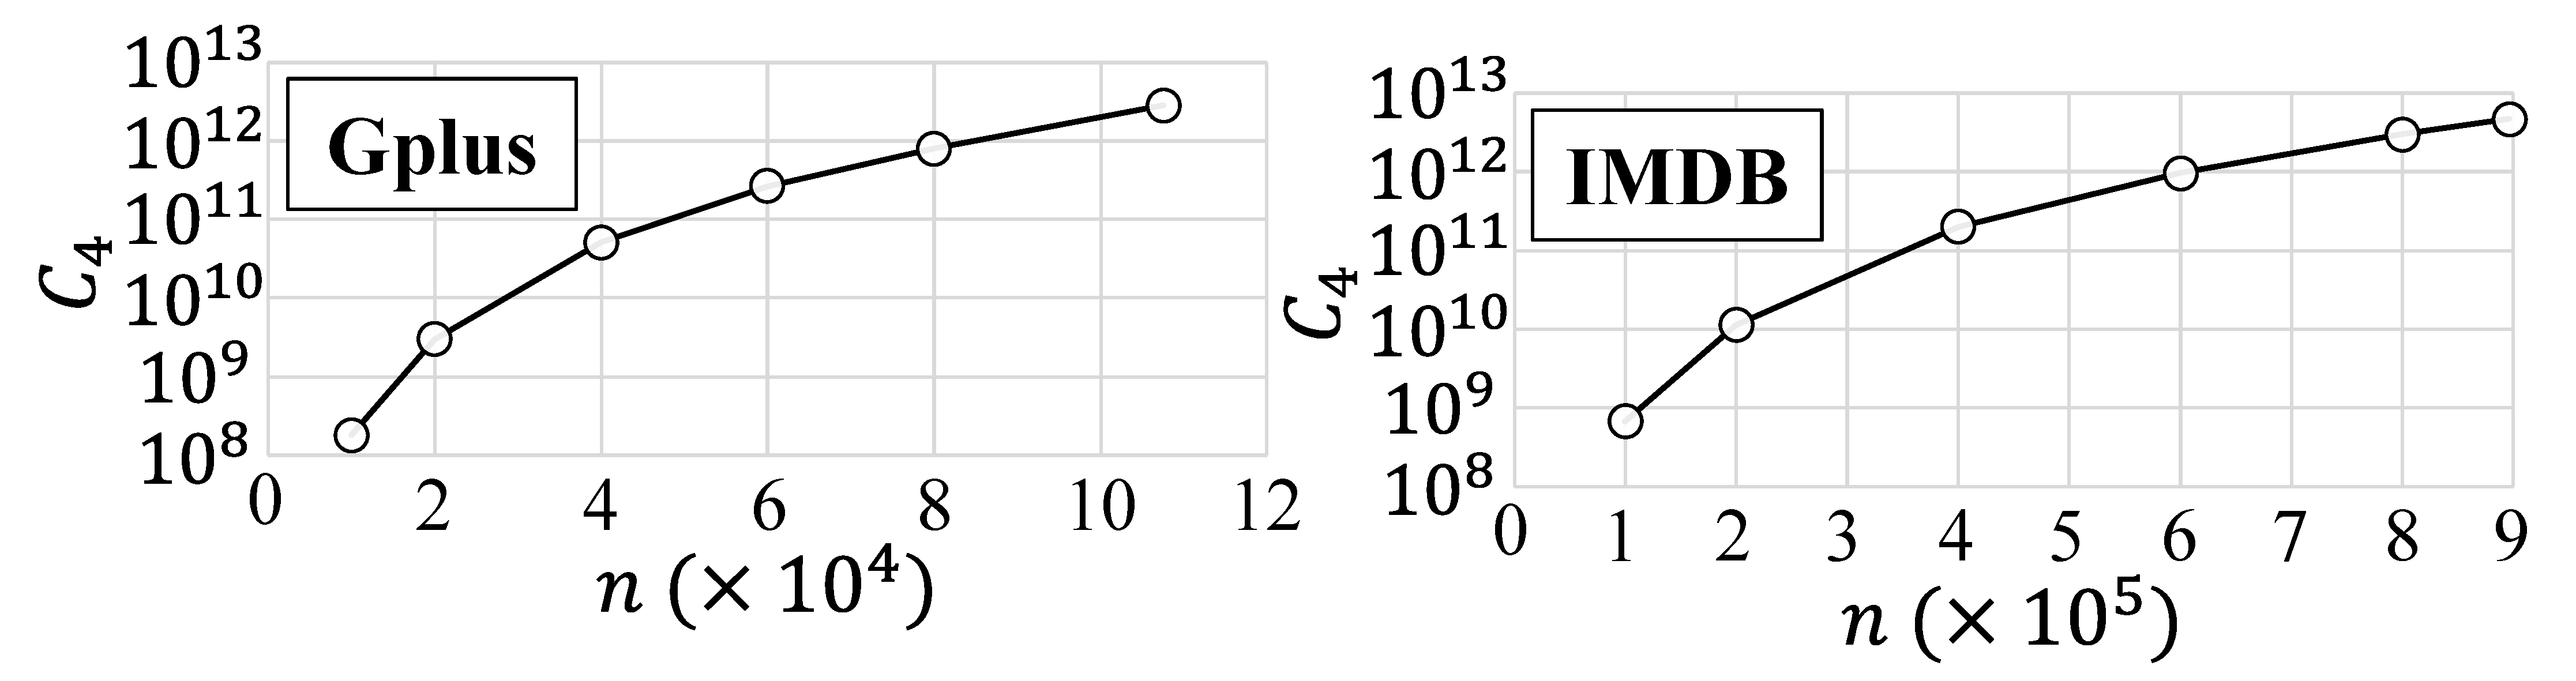
\includegraphics[width=0.99\linewidth]{fig/res4_4cycles.pdf}
  \vspace{-5mm}
%   \caption{Maximum degree $d_{max}$ and \#$4$-cycles $C_4$.} 
  \caption{\#$4$-cycles $C_4$.} 
  \label{chap2-fig:res4_4cycles}
\end{figure}

Based on Figures~\ref{chap2-fig:res3_emp_Lap} and \ref{chap2-fig:res4_4cycles}, we can explain 
% the results in 
Figure~\ref{chap2-fig:res3_n} as follows. 
As shown in Section~\ref{chap2-sub:clip_theoretical_analysis}, the $l_2$ loss of empirical estimation can be expressed as 
% $O(\frac{n d_{max}^3}{\mu_F})$, $O(\frac{n d_{max}^2}{\mu_O^2})$, and $O(\frac{n d_{max}^2}{\mu_T^3})$ 
$O(n d_{max}^3)$, $O(n d_{max}^2)$, and $O(n d_{max}^2)$ 
in \AlgOne{}, \AlgTwo{}, and \AlgThree{}, respectively. 
% when 
% we regard $\epsilon$ as a constant.
% $\mu_F$ ($= \mu_O^2 = \mu_T^3$) 
% $\mu^*$ is small.  
The large $l_2$ loss of \AlgOne{} is caused by a large value of $C_4$. 
% as shown in Figure~\ref{chap2-fig:res4_4cycles}. 
% the $4$-cycle issue. 
% When 
% $\mu_F$ is small, 
% $n$ is small, 
% the Laplacian noise has a non-negligible impact on the estimation error. 
% as explained in Section~\ref{chap2-sub:clip_theoretical_analysis}. 
% However, 
The expected $l_2$ loss of the Laplacian noise is 
$O(\sum_{i=1}^n \kappa_i^2)$, 
% $O(\sum_{i=1}^n \lambda_i^2 \td_i^2)$, 
which is much smaller than $O(n d_{max}^2)$. 
Thus, 
% when $n$ is large, 
as $n$ increases, 
% when $d_{max}$ is proportional to $n$, 
% as in Figure~\ref{chap2-fig:res4_4cycles}, 
the Laplacian noise becomes relatively very small, 
% rapidly decreases with increase in $n$ 
as shown in Figure~\ref{chap2-fig:res3_emp_Lap}. 
Consequently, \AlgTwo{} provides the best performance for large $n$ because it addresses the $4$-cycle issue 
and effectively reduces the global sensitivity. 
This explains the results in Figure~\ref{chap2-fig:res3_n}. 
It is also interesting that when $n \approx 10^5$, \AlgOne{} performs the worst in \GPlus{} and almost the same as \AlgTwo{} in \IMDB{} (see Figure~\ref{chap2-fig:res3_n}). 
This is because \GPlus{} is more dense than \IMDB{} 
% (as described in Section~\ref{chap2-sub:setup}) 
and $C_4$ is much larger in \GPlus{} when $n \approx 10^5$, as in Figure~\ref{chap2-fig:res4_4cycles}.

In other words, Figures~\ref{chap2-fig:res3_n}, \ref{chap2-fig:res3_emp_Lap}, and \ref{chap2-fig:res4_4cycles} are consistent with our theoretical results in Section~\ref{chap2-sub:clip_theoretical_analysis}. 
From these results, we conclude that \AlgTwo{} is effective especially for 
a large graph (e.g., $n \approx 10^6$) or dense graph (e.g., \GPlus{}) where the number $C_4$ of $4$-cycles is large. 
% a graph that has a large number of $4$-cycles. 
% In Appendix~\ref{chap2-sec:BAmodel}, we also show similar results using the Barab\'{a}si-Albert graph model.



% \smallskip
% \noindent{\textbf{Communication Cost.}}~~TBD.

\smallskip
\noindent{\textbf{Summary.}}~~In summary, our answers to our three research questions RQ1-3 
% at the beginning of Section~\ref{chap2-sec:experiments} 
are as follows. 
% \begin{itemize}
%     \item Our 
% \end{itemize}
% First, 
[RQ1]: Our \AlgTwo{} achieves almost the smallest estimation error in all cases and outperforms the other two, especially for a large graph or dense graph where $C_4$ is large. 
[RQ2]: Our double clipping reduces the estimation error by two or three orders of magnitude. 
[RQ3]: Our entire algorithm (\AlgTwo{} with double clipping) dramatically reduces the communication cost, 
e.g., 
% from $400$ Gbits to $160$ Mbits or less (relative error $=0.21$) in \IMDB{}.
% When the DL speed is $20$ Mbps \cite{YouTube_speed}, the DL time is reduced from $6$ hours to $5$ seconds. 
from $6$ hours to $8$ seconds or less (relative error $=0.21$) in \IMDB{} at a $20$ Mbps download rate \cite{YouTube_speed}. 

Thus, triangle counting under edge LDP is now 
much more 
practical. 
In Appendix~\ref{chap2-sec:cluster}, we show that the clustering coefficient can also be accurately estimated using our algorithms.


\section{Conclusions}
\label{sec:conclusions}
% In this paper, we proposed
% locally private
We proposed
triangle counting algorithms under edge LDP with a small estimation error and small communication cost.
We showed that
% the estimation error can be significantly reduced by our 4-cycle trick and double clipping, and that
our entire algorithms with the 4-cycle trick and double clipping
% can 
dramatically reduce the download cost
% when compared with
of
\cite{Imola_USENIX21},
% (e.g., from $400$ Gbits to $100$ Mbits).
e.g., from 6 hours to 8 seconds or less. 
% when $20$ Mbps).
% In \cite{Imola_USENIX21},

% In this paper,
We assumed that each user $v_i$ honestly inputs her neighbor list $\bma_i$, as in most previous work on LDP.
However, recent studies \cite{Cao_USENIX21,Cheu_SP21} show that the estimate in LDP can be skewed by data poisoning attacks.
% with a number of malicious accounts.
As future work, we would like to analyze the impact of data poisoning on our algorithms and develop defenses (e.g., detection) against it.


% %-------------------------------------------------------------------------------
\section*{Acknowledgments}
Kamalika Chaudhuri and Jacob Imola would like to thank ONR under N00014-20-1-2334 and UC Lab Fees under LFR 18-548554  for research support.
Takao Murakami was supported in part by JSPS KAKENHI JP19H04113.



\graphicspath{{./chapters/chapter3/}}

\chapter{Differentially Private Triangle and 4-Cycle Counting in the Shuffle Model}\label{chap:3}

\newcommand{\MSE}{\operatorname{\textsf{MSE}}}

% \def\AlgWS{\textsf{WShuffle}$_{i,j}$}
\def\AlgWS{\textsf{WS}}
\def\AlgWSLE{\textsf{WSLE}}
\def\AlgWSTri{\textsf{WShuffle}$_{\triangle}$}
% \def\AlgWSTri{\textsf{WSLE}$_{\triangle}$}
\def\AlgWSTriVR{\textsf{WShuffle}$_{\triangle}^*$}
% \def\AlgWSTriVR{\textsf{WSLE}$_{\triangle}^*$}

\def\AlgWLTri{\textsf{WLocal}$_{\triangle}$}
\def\AlgARRTri{\textsf{ARR}$_{\triangle}$}
\def\AlgRRTri{\textsf{RR}$_{\triangle}$}
\def\AlgTwoRL{\textsf{2R-Large}$_{\triangle}$}
\def\AlgTwoRS{\textsf{2R-Small}$_{\triangle}$}

\def\AlgWSCyc{\textsf{WShuffle}$_{\square}$}
\def\AlgWLCyc{\textsf{WLocal}$_{\square}$}


\section{Introduction}
\label{chap3-sec:intro}
Graph statistics is useful for finding meaningful connection patterns in network data, and 
% counting subgraphs (e.g., triangles, $k$-stars, cycles, cliques) 
subgraph counting is known as a fundamental task in graph analysis. 
For example, a triangle is a cycle of size three, 
% consists of three nodes with three edges, 
and a $k$-star consists of a central node connected to $k$ other nodes.  
These subgraphs 
% important because they 
can be used to calculate 
a 
% (global) 
clustering coefficient ($=\frac{3 \times \text{\#triangles}}{\text{\#2-stars}}$). 
In a social graph, the clustering coefficient measures 
the tendency of nodes (users) to form a cluster with each other. 
% the degree to which nodes (users) tend to cluster together 
It also represents the average probability that a friend's friend is also a friend \cite{Newman_PRL09}. 
% two friends of a user will also be a friend 
Therefore, the clustering coefficient is useful for analyzing the effectiveness of friend suggestions. 
% For another example, a 4-cycle is a cycle composed of four nodes 
Another example of the subgraph is a 4-cycle, 
% which is a cycle composed of four nodes. 
a cycle of size four. 
The 4-cycle count is useful for measuring the clustering ability in bipartite graphs (e.g., 
% sexual contact networks \cite{Lind_PRE05}) 
online dating networks, mentor-student networks \cite{Kutty_WWW14}) 
where a triangle never appears \cite{Lind_PRE05,Robins_CMOT04,Sanei-Mehri_CIKM19}. 
Figure~\ref{chap3-fig:subgraphs} shows examples of triangles, 2-stars, and 4-cycles. 
% 
% Although subgraph counts are important for analyzing the connection patterns or clustering tendency, they can leak sensitive edges (friendships). 
Although these subgraphs are important for analyzing the connection patterns or clustering tendencies, their exact numbers can leak sensitive edges (friendships) \cite{Imola_USENIX21}. 
%include sensitive data such as sensitive friendships. 
% For example, in Figure~XX, the triangle count 

\begin{figure}[t]
  \centering
  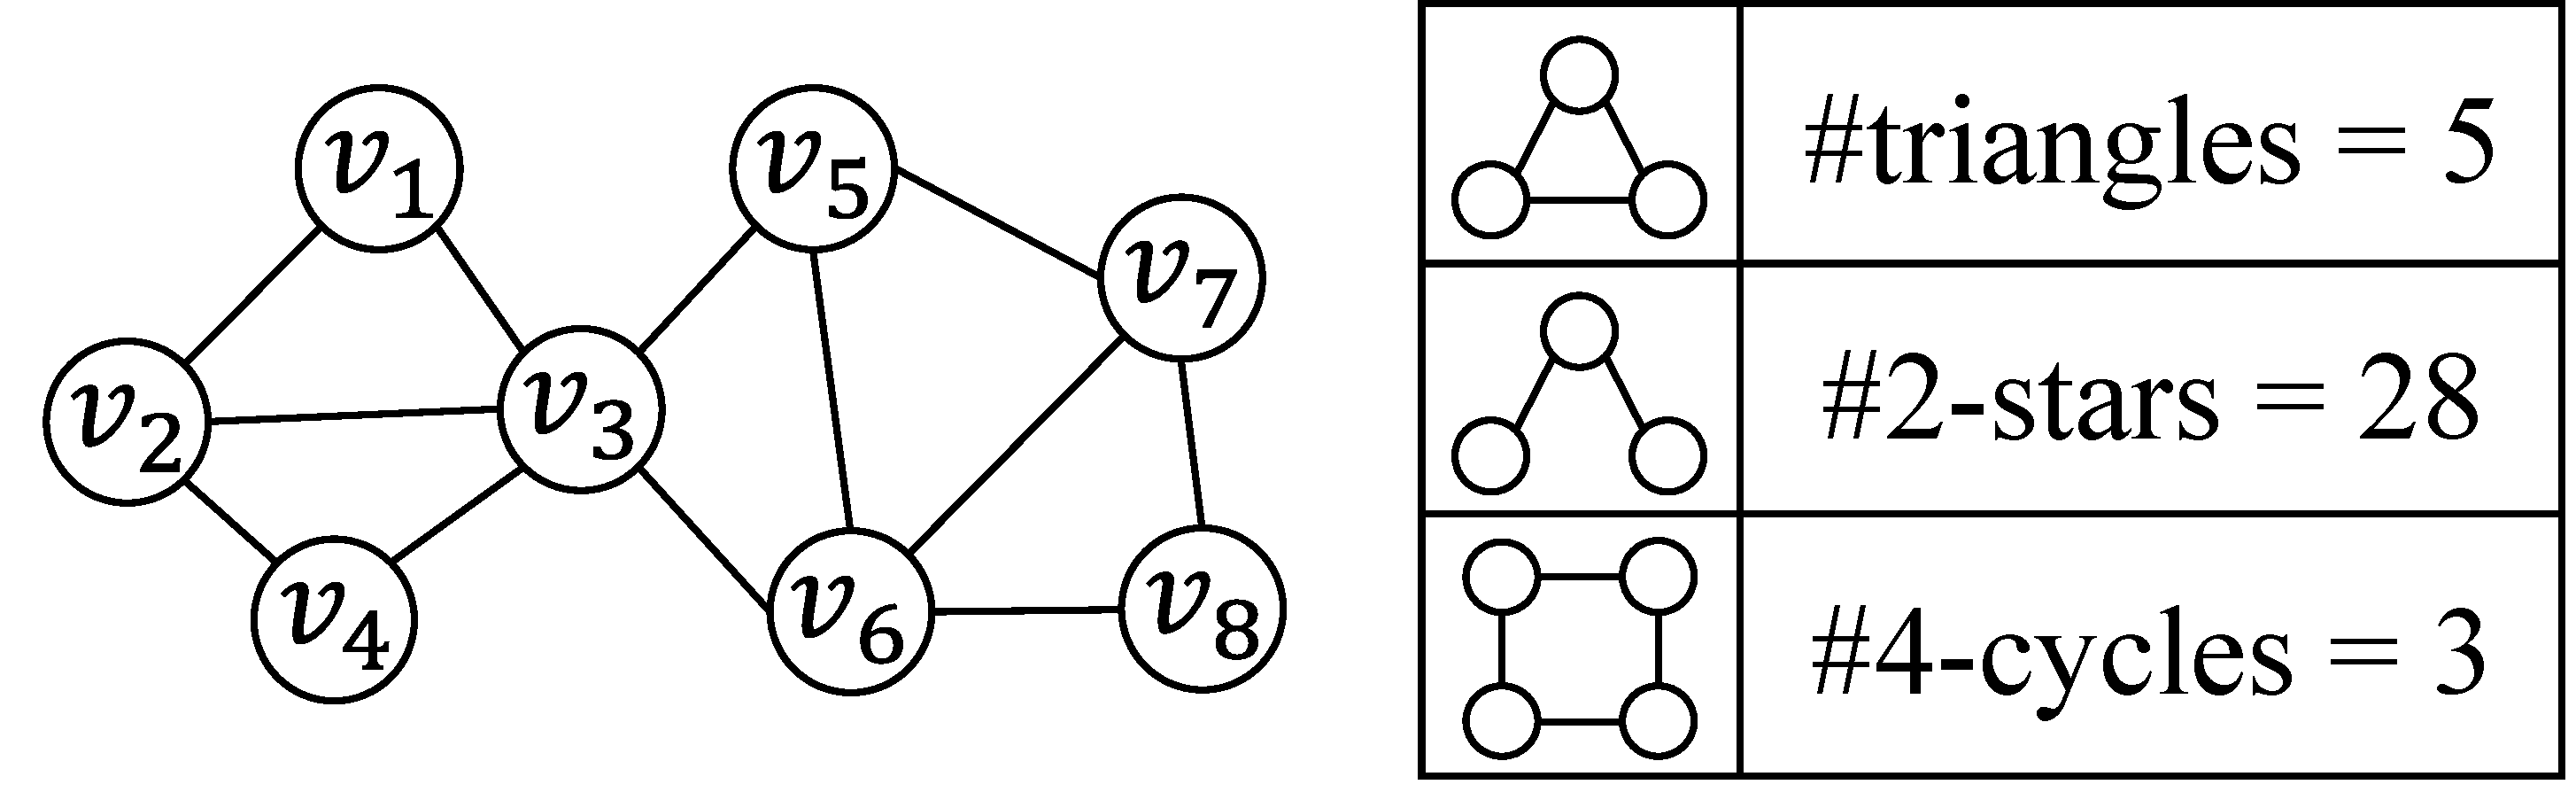
\includegraphics[width=0.65\linewidth]{fig/subgraphs.pdf}
  
  \caption[Examples of subgraph counts.]{Examples of subgraph counts.
  }
  \label{chap3-fig:subgraphs}
\end{figure}

DP (Differential Privacy) \cite{Dwork_ICALP06,DP} -- the gold standard of privacy notions -- has been widely used to strongly protect edges in graph data \cite{Day_SIGMOD16,Ding_TKDE21,Hay_ICDM09,Imola_USENIX21,Imola_USENIX22,Karwa_PVLDB11,Kasiviswanathan_TCC13,qin2017generating,Sun_CCS19,Ye_ICDE20,Ye_TKDE21}. 
% DP strongly protects user privacy when a parameter (privacy budget) $\epsilon$ is small and is known as the gold standard of privacy notions. 
% against adversaries with any background knowledge. 
In particular, recent studies 
\cite{Imola_USENIX21,Imola_USENIX22,qin2017generating,Ye_ICDE20,Ye_TKDE21} 
% \cite{Imola_USENIX21,Imola_USENIX22,Ye_ICDE20,Ye_TKDE21} 
have applied LDP (Local DP) \cite{Kasiviswanathan_FOCS08} to 
graph data. 
% subgraph counting. 
% where each user has 
%subgraph counting. 
In the graph LDP model, each user obfuscates her neighbor list (friends list) by herself and sends the obfuscated neighbor list to a data collector. 
Then, the data collector estimates graph statistics, such as subgraph counts. 
Compared to central DP where a central server has personal data of all users (i.e., the entire graph), LDP does not have a risk that all personal data are leaked from the server by 
% illegal access 
cyberattacks 
\cite{Henriquez_breach2021} or insider attacks \cite{Kohen_insider_threats}. 
Moreover, LDP can be applied to decentralized social networks \cite{Paul_CN14,Salve_CSR18} (e.g., diaspora* \cite{Diaspora}, Mastodon \cite{Mastodon}) where no server can access the entire graph; e.g., 
the entire graph is distributed across many servers, or no server has any original edges. 
It is reported in \cite{Imola_USENIX21} that $k$-star counts can be accurately estimated in this model. 

However, it is much more challenging to accurately count more complicated subgraphs such as triangles and 4-cycles under LDP. 
The root cause of this is its local property -- a user cannot see edges between others. 
% For example, user $v_3$ knows that there are ten $2$-stars of which she is a center. 
% However, $v_3$ cannot count triangles or 4-cycles including $v_3$, as she cannot see edges between others, e.g., $(v_1,v_2)$ and $(v_2,v_4)$. 
For example, user $v_1$ cannot count triangles or 4-cycles including $v_1$, as she cannot see edges between others, e.g., $(v_2,v_3)$, $(v_2,v_4)$, and $(v_3,v_4)$. 
Therefore, the existing algorithms \cite{Imola_USENIX21,Imola_USENIX22,Ye_ICDE20,Ye_TKDE21} 
obfuscate 
each bit of the neighbor list 
% each user's edges 
rather than the subgraph count by 
% apply 
% Warner's 
the RR (Randomized Response) \cite{Warner_JASA65}, which randomly flips 0/1. 
% with some probability, 
% to each bit of the neighbor list. 
As a result, their algorithms suffer from extremely large estimation errors because it makes all edges noisy. 
% any triangle or 4-cycle. 
% To address this issue, 
Some studies \cite{Imola_USENIX21,Imola_USENIX22} 
significantly improve the accuracy by introducing 
% introduce 
an additional round of interaction between users and the data collector. 
% Their algorithms publish the noisy graph at the first round to enable each user to count her triangles such that only one edge is noisy at the second round. 
% In their algorithms, the data collector publishes the noisy graph at the first round. 
% Specifically, they propose triangle algorithms that publish the noisy graph at the first round 
% so that each user can count her triangles at the second round. 
% Then, at the second round, each user can count her triangles such that only one edge is noisy. 
% because she knows two edges connected to her. 
% Therefore, the accuracy is significantly improved. 
% Thus, the two-rounds algorithms significantly reduce the estimation error. 
However, multi-round interaction may be impractical in many applications, as it requires a lot of user effort and synchronization; 
in  \cite{Imola_USENIX21,Imola_USENIX22}, every user must respond twice, and the data collector must wait for responses from all users 
in each round. 
% to publish the noisy graph. 

In this work, we focus on a \textbf{one-round} of interaction between users and the data collector and propose accurate subgraph counting algorithms by introducing a recently studied privacy model: the \textit{shuffle model} \cite{Erlingsson_SODA19,Feldman_FOCS21}. 
% The shuffle model introduces an intermediate server called the shuffler. 
In the shuffle model, each user sends her (encrypted) obfuscated data to an intermediate server called the shuffler. 
Then, the shuffler randomly shuffles the obfuscated data of all users and sends the shuffled data to the data collector (who decrypts them). 
% It has been proven that 
The shuffling amplifies DP guarantees of the obfuscated data under the assumption that the shuffler and the data collector do not collude with each other. 
Specifically, it is known that DP strongly protects user privacy when a parameter (a.k.a. privacy budget) $\epsilon$ is small, e.g., $\epsilon \leq 1$ \cite{DP_Li}. 
The shuffling significantly reduces $\epsilon$ and therefore significantly improves utility at the same value of $\epsilon$. 
To date, the shuffle model has been successfully applied to tabular data \cite{Meehan_ICLR22,Wang_PVLDB20} and 
% image data 
gradients \cite{Girgis_AISTATS21,Liu_AAAI21} in federated learning. 
We 
%make the first attempt (to our knowledge) to apply the shuffle model to subgraph counting. 
apply the shuffle model to graph data to accurately count subgraphs within one round. 
%one-round subgraph counting to provide a small estimation error. 

% However, it is very challenging to apply the shuffle model to subgraph counting because 
The main challenge in subgraph counting in the shuffle model is that each user's neighbor list is \textit{high-dimensional data}, i.e., $n$-dim binary string where $n$ is the number of users. 
% we cannot use the entire neighbor list as input data. 
Consequently, applying the RR to each bit of the neighbor list, as in the existing work \cite{Imola_USENIX21,Imola_USENIX22,Ye_ICDE20,Ye_TKDE21}, results in an extremely large privacy budget $\epsilon$ even after applying the shuffling (see Section~\ref{chap3-sub:technical} for more details). 

We address this issue by introducing a new, basic technique called \textit{wedge shuffling}. 
In graphs, a wedge between $v_i$ and $v_j$ is defined by a 2-hop path with endpoints $v_i$ and $v_j$. 
% Our wedge shuffle technique obfuscates a wedge (2-hop path) between a specific user-pair. 
% rather than the entire neighbor list. 
For example, in Figure~\ref{chap3-fig:subgraphs}, 
there are two wedges between $v_2$ and $v_3$: $v_2$-$v_1$-$v_3$ and $v_2$-$v_4$-$v_3$. 
In other words, users $v_1$ and $v_4$ have a wedge between $v_2$ and $v_3$, whereas $v_5, \ldots, v_8$ do not. 
Each user obfuscates such wedge information by the RR, and the shuffler randomly shuffles them. 
Because the wedge information (i.e., whether there is a wedge between a specific user-pair) 
is \textit{one-dimensional binary data}, it can be sent with small noise and small $\epsilon$. 
In addition, the wedge is the main component of several subgraphs, such as triangles, 4-cycles, and 3-hop paths \cite{Sun_CCS19}. 
Since the wedge has little noise, we can accurately count these subgraphs based on wedge shuffling. 

We apply wedge shuffling to triangle and 4-cycle counting tasks with several additional techniques. 
For triangles, we first 
%consider a problem of counting 
propose an algorithm that counts triangles involving the user-pair at the endpoints of the wedges by locally sending an edge between the user-pair to the data collector. 
% along with shuffled wedges. 
% to count triangles including the user-pair. 
Then we propose an algorithm to count triangles in the entire graph by sampling disjoint user-pairs, which share no common users (i.e., 
no user falls in two pairs). 
We also propose a technique to reduce the variance of the estimate by ignoring sparse user-pairs, where either of the two users has a very small degree. 
For 4-cycles, we propose an algorithm to calculate an unbiased estimate of the 4-cycle count from that of the wedge count via bias correction. 

% We propose triangle and 4-cycle counting algorithms based on our wedge shuffle technique and show upper bounds on the estimation error for our algorithms. 
We provide upper bounds on the estimation error for our triangle and 4-cycles counting algorithms. 
Through comprehensive evaluation, we show that 
% it is possible to accurately estimate 
our algorithms 
accurately estimate these subgraph counts within one round under the shuffle model. 
% to triangles and 4-cycles. 
% with some additional techniques. 
% Our experimental results show that 

% \begin{itemize}
%     \item shuffle model for graphs?
%     \item define graph shuffle model
%     \item problem: high dim data
%     \item counting triangles/4-cycles
%     \item our approach: dim reduction by wedges
% \end{itemize}


\smallskip
\noindent{\textbf{Our Contributions.}}~~Our contributions are as follows: 
\begin{itemize}
    \item We propose a wedge shuffle technique to enable privacy amplification 
    %in subgraph counting. 
    of graph data. 
    To our knowledge, we are the first to shuffle graph data (see Section~\ref{chap3-sec:related} for more details). 
    %apply the shuffle model to graph data. 
    \item We propose one-round triangle and 4-cycle counting algorithms 
    %with theoretical performance guarantees 
    based on our wedge shuffle technique. 
    %apply wedge shuffling to triangles and 4-cycles. 
    For triangles, we propose three additional techniques: sending local edges, sampling disjoint user-pairs, and variance reduction by ignoring sparse user-pairs. 
    For 4-cycles, we propose a bias correction technique. 
    We show upper bounds on the estimation error for each algorithm. 
    \item We evaluate our algorithms using two real graph datasets. 
    Our experimental results show that our one-round shuffle algorithms 
    significantly outperform one-round local algorithms in terms of accuracy 
    %dramatically the estimation error of the one-round local algorithms 
    and achieve a small estimation error (relative error $\ll 1$) with a reasonable privacy budget, e.g., smaller than $1$ in edge DP. 
\end{itemize}
In \conference{the full version of this paper \cite{Imola_CCSFull22}}\arxiv{Appendix~\ref{chap3-sec:cluster}}, we show that our triangle algorithm is also useful for accurately estimating the clustering coefficient within one round. 
% we can also accurately estimate the clustering coefficient within one round by using our triangle algorithm. 
We can use our algorithms to analyze the clustering tendency or the effectiveness of friend suggestions in decentralized social networks by introducing a shuffler. 
We implemented our algorithms in C/C++. 
Our code is available on GitHub \cite{SubgraphShuffle}. 
The proofs of all statements in the main body are given in \conference{\cite{Imola_CCSFull22}}\arxiv{Appendices~\ref{chap3-sec:triangle_proof} and \ref{chap3-sec:4cycle_proof}}. 

\section{Related Work}
\label{sec:related}
% \smallskip
\noindent{\textbf{Non-private Subgraph Counting.}}~~Subgraph counting has been extensively studied in a non-private setting (see \cite{Ribeiro_CS21} for a recent survey). 
% Differentially priate graph analysis has been widely studied in the literature. 
% In particular, triangle counting is considered one of the most basic task 
Examples of subgraphs include triangles \cite{Bera_PODS20,Eden_FOCS15,Kolountzakis_IM12,Wu_TKDE16},  4-cycles \cite{Bera_STACS17,Kallaugher_PODS19,Manjunath_ESA11,McGregor_PODS20}, $k$-stars \cite{Aliakbarpour_Alg18,Gonen_DM11}, and 
$k$-hop paths \cite{Bjorklund_ICALP19,Kartun-Giles_TWC18}. 

Here, the main challenge is to reduce the computational time of counting these subgraphs in large-scale graph data. 
One of the simplest approaches is edge sampling \cite{Bera_PODS20,Eden_FOCS15,Wu_TKDE16}, which randomly 
% and independently 
samples edges in a graph. 
Edge sampling outperforms other sampling methods 
% approaches 
(e.g., node sampling, triangle sampling) \cite{Wu_TKDE16} and is also adopted in \cite{Imola_USENIX22} 
% to improve communication efficiency in 
for private triangle counting. 

Although our triangle algorithm also samples user-pairs, ours is different from edge sampling in two ways. 
First, our algorithm does not sample an edge but samples a pair of users who may or may not be a friend. 
% have an edge between them. 
Second, our algorithm samples user-pairs that share no common users to avoid the increase of the privacy budget $\epsilon$ as well as to reduce the time complexity 
(see Section~\ref{sec:triangle} for details). 

\smallskip
\noindent{\textbf{Private Subgraph Counting.}}~~Differentially private subgraph counting has been widely studied, and the previous work assumes either the central \cite{Ding_TKDE21,Karwa_PVLDB11,Kasiviswanathan_TCC13} or local \cite{Imola_USENIX21,Imola_USENIX22,Sun_CCS19,Ye_ICDE20,Ye_TKDE21} models. 
The central model assumes a centralized social network and has a data breach issue, as explained in Section~\ref{sec:intro}. 

Subgraph counting in the local model has recently attracted attention. 
Sun \textit{et al.} \cite{Sun_CCS19} propose subgraph counting algorithms 
% under the assumption 
assuming 
that each user knows all friends' friends. 
However, this assumption does not hold in many social networks; e.g., Facebook users can change their settings so that anyone cannot see their friend lists. 
Therefore, we make a minimal assumption -- each user knows only her friends. 

% Some studies \cite{Imola_USENIX21,Imola_USENIX22,Ye_ICDE20,Ye_TKDE21} focus on this setting. 

In this setting, recent studies propose triangle \cite{Imola_USENIX21,Imola_USENIX22,Ye_ICDE20,Ye_TKDE21} and $k$-star \cite{Imola_USENIX21} counting algorithms. 
% As described in Section~\ref{sec:intro}, 
For $k$-stars, Imola \textit{et al.} \cite{Imola_USENIX21} propose a one-round algorithm that is order optimal and show that it provides a very small estimation error. 
% Triangles are much more challenging than $k$-stars. 
% Ye \textit{et al.} \cite{Ye_ICDE20} propose a one-round algorithm that applies the RR to each bit of the neighbor list and then counts the number of triangles in the noisy graph. 
% They also propose an algorithm to reduce the bias in the estimate \cite{Ye_TKDE21} (though there is no proof that the estimate is unbiased). 
% Imola \textit{et al.} \cite{Imola_USENIX21} 
For triangles, they
propose a one-round algorithm that applies the RR to 
% bits for smaller user IDs in 
each bit of the neighbor list 
and then calculates an unbiased estimate of triangles from the noisy graph. 
We call this algorithm \AlgRRTri{}. 
Imola \textit{et al.} \cite{Imola_USENIX22} show that \AlgRRTri{} provides a much smaller estimation error than the one-round triangle algorithms in \cite{Ye_ICDE20,Ye_TKDE21}. 
In \cite{Imola_USENIX22}, they also reduce the time complexity of \AlgRRTri{} 
% from $O(n^3)$ to $O(n^2)$ 
by using the ARR (Asymmetric RR), which samples each 1 (edge) after applying the RR. 
We call this algorithm \AlgARRTri{}. 
In this paper, we use \AlgRRTri{} and \AlgARRTri{} as baselines in triangle counting. 
% compare our triangle algorithms with \AlgRRTri{} and \AlgARRTri{} in our theoretical analysis and with \AlgARRTri{} in our experiments (we cannot apply \AlgRRTri{} to large-scale graphs, as it is too inefficient; see ). 
For 4-cycles, there is no existing algorithm under LDP, to our knowledge. 
Thus, we compare our shuffle algorithm with its local version, which does not shuffle the obfuscated data. 

For triangles, Imola \textit{et al.} also propose a two-round local algorithm in \cite{Imola_USENIX21} and significantly reduce its download cost in \cite{Imola_USENIX22}. 
Although we focus on one-round algorithms, 
% as described in Section~\ref{sec:intro}. 
we show in 
% Section~\ref{sec:experiments} 
\conference{the full version \cite{Imola_CCSFull22}}\arxiv{Appendix~\ref{sec:two-round}} 
that our one-round algorithm is comparable to the two-round algorithm in \cite{Imola_USENIX22}, which requires a lot of user effort and synchronization, in terms of accuracy. 

% In this paper, we compare our triangle algorithms with \AlgRRTri{} and \AlgARRTri{} in our theoretical analysis and with \AlgARRTri{} in our experiments (we cannot apply \AlgRRTri{} to large-scale graphs, as it is too inefficient; see ). 

% one-round local triangle counting \cite{Imola_USENIX21,Imola_USENIX22,Ye_ICDE20,Ye_TKDE21}, \AlgARRTri{} \cite{Imola_USENIX22}, \AlgRRTri{} \cite{Imola_USENIX21}. Explain  and \AlgARRTri{} in detail because they are compared with our algorithms.

\smallskip
\noindent{\textbf{Shuffle Model.}}~~The privacy amplification by shuffling has been recently studied in \cite{Balle_CRYPTO19,Cheu_EUROCRYPT19,Erlingsson_SODA19,Feldman_FOCS21}. 
Among them, the privacy amplification bound by Feldman \textit{et al.} \cite{Feldman_FOCS21} is the state-of-the-art -- it provides a smaller $\epsilon$ than other bounds, such as \cite{Balle_CRYPTO19,Cheu_EUROCRYPT19,Erlingsson_SODA19}. 
%and is more general than the bound in \cite{Cheu_EUROCRYPT19} that is specific to binary RR. 
Girgis \textit{et al.} \cite{Girgis_CCS21} 
consider multiple interactions between users and the data collector and 
show a better bound than the bound in \cite{Feldman_FOCS21} when used with composition. 
However, the bound in \cite{Feldman_FOCS21} outperforms the bound in \cite{Girgis_CCS21} when used without composition. 
% (which is the case with this work that considers a single interaction). 
Because our work focuses on a single interaction and does not use the composition, 
% Therefore, 
we use the bound in \cite{Feldman_FOCS21}. 

The shuffle model has been applied to tabular data \cite{Meehan_ICLR22,Wang_PVLDB20} and gradients \cite{Girgis_AISTATS21,Liu_AAAI21} in federated learning. 
Meehan \textit{et al.} \cite{Meehan_ICLR22} construct a graph from public auxiliary information and determine a permutation of obfuscated data using the graph to reduce re-identification risks. 
Liew \textit{et al.} \cite{Liew_SIGMOD22} propose network shuffling, which shuffles obfuscated data via random walks on a graph. 
%, where users exchange their obfuscated data 
%each user relays her obfuscated data to her neighbor
Note that both \cite{Meehan_ICLR22} and \cite{Liew_SIGMOD22} use graph data to shuffle another type of data. 
% neither \cite{Meehan_ICLR22} or \cite{Liew_SIGMOD22} shuffles graph data itself (they shuffle another data using graph data). 
To our knowledge, our work is the first to shuffle graph data itself. 

\section{Preliminaries}
\label{chap3-sec:preliminaries}
In this section, we describe some preliminaries for our work. 
Section~\ref{chap3-sub:notations} defines the basic notation used in this paper. 
% Sections~\ref{chap3-sub:privacy} and \ref{chap3-sub:utility} explain privacy notions and utility metrics, respectively. 
Sections~\ref{chap3-sub:privacy} and \ref{chap3-sub:shuffle} introduce DP on graphs and the shuffle model, respectively. 
Section~\ref{chap3-sub:utility} explains utility metrics. 

\subsection{Notation}
\label{chap3-sub:notations}
Let $\reals$, $\nnreals$, $\nats$, and $\nnints$ be the sets of real numbers, non-negative real numbers, natural numbers, and non-negative integers, respectively. 
% For $z\in\reals$, let $[z]$ be the set of natural numbers that do not exceed $z$. 
For $a\in\nats$, let $[a]$ be the set of natural numbers that do not exceed $a$, i.e., $[a] = \{1, 2, \ldots, a\}$. 
% Let $I_{-(i,j)} = [n]\setminus\{i,j\}$. 

We consider an undirected social graph $G=(V,E)$, where $V$ represents a set of nodes (users) and $E \subseteq V \times V$ represents a set of edges (friendships). 
Let $n\in\nats$ be the number of nodes in $V$, and $v_i \in V$ be the $i$-th node, i.e., $V=\{v_1,\ldots,v_n\}$. 
Let $I_{-(i,j)}$ be the set of indices of users other than $v_i$ and $v_j$, i.e., $I_{-(i,j)} = [n]\setminus\{i,j\}$. 
Let 
$d_i \in \nnints$ be a degree of $v_i$, 
$d_{avg} \in \nnreals$ be the average degree of $G$, and $d_{max} \in \nats$ be the maximum degree of $G$. 
In most real graphs, $d_{avg} \ll d_{max} \ll n$ holds. 
We denote a set of graphs with $n$ nodes by $\calG$. 
Let $f^\triangle: \calG \rightarrow \nnints$ and $f^\square: \calG \rightarrow \nnints$ be triangle and 4-cycle count functions, respectively. 
% Let $f^\triangle: \calG \rightarrow \nnints$ be a triangle count query. 
The triangle count function takes $G \in \calG$ as input and outputs the number $f^\triangle(G)$ of triangles in $G$, 
whereas the 4-cycle count function takes $G$ as input and outputs the number $f^\square(G)$ of 4-cycles. 
% Let $\hf^\triangle: \calG \rightarrow \reals$ be a triangle count estimator, which takes $G$ as input and outputs the estimate $\hf^\triangle(G)$ of triangles. 

Let $\bmA=(a_{i,j}) \in \{0,1\}^{n \times n}$ be 
%a symmetric 
an adjacency matrix corresponding to $G$. 
% $a_{i,j} = 1$ if and only if $(v_i,v_j) \in E$. 
If $(v_i,v_j) \in E$, then $a_{i,j} = 1$; otherwise, $a_{i,j} = 0$. 
We call $a_{i,j}$ an \textit{edge indicator}. 
Let $\bma_i \in \{0,1\}^n$ be a neighbor list of user $v_i$, i.e., the $i$-th row of $\bmA$. 
\arxiv{Table~\ref{chap3-tab:notations} shows the basic notation in this paper.} 
% We summarize the basic notation in Table~\ref{chap3-tab:notations} of Appendix~\ref{chap3-sec:notation_table}.

\arxiv{\begin{table}[t]
\caption[Basic notation in this paper.]{Basic notation in this paper.}

\centering
\hbox to\hsize{\hfil
\begin{tabular}{l|l}
\hline
Symbol		&	Description\\
\hline
% $I_{-(i,j)}$    &   Set of user indices other than $i$ and $j$ ($[n]\setminus\{i,j\}$).\\
$G=(V,E)$   &	    Undirected social graph.\\
$n$         &	    Number of nodes (users).\\
$v_i$       &       $i$-th user in $V$, i.e., $V=\{v_1,\ldots,v_n\}$.\\
% $I_{-(i,j)}$    &   Set of user indices other than $i$ and $j$ ($[n]\setminus\{i,j\}$).\\
$I_{-(i,j)}$    &   $=[n]\setminus\{i,j\}$.\\
$d_i$   &       Degree of $v_i$.\\
$d_{avg}$   &       Average degree in $G$.\\
$d_{max}$   &       Maximum degree in $G$.\\
$\calG$     &       Set of possible graphs with $n$ nodes.\\
$f^\triangle(G)$   &  Triangle count in graph $G$.\\
$f^\square(G)$   &  4-cycle count in graph $G$.\\
% $\hf^\triangle(G)$   &  Estimate of the triangle count in graph $G$.\\
$\bmA=(a_{i,j})$	    &		Adjacency matrix.\\
% $a_{i,j}$	&		Edge indicator between $v_i$ and $v_j$.\\
$\bma_i$	&		Neighbor list of $v_i$, i.e., the $i$-th row of $\bmA$.\\
% $\calR_i$     &       Local randomizer of $v_i$.\\
\hline
\end{tabular}
\hfil}
\label{chap3-tab:notations}
\end{table}}

% \subsection{Privacy Notions}
\subsection{Differential Privacy}
\label{chap3-sub:privacy}
% \smallskip
% \noindent{\textbf{$(\epsilon,\delta)$-DP.}}~~
\noindent{\textbf{DP and LDP.}}~~We use differential privacy, and more specifically $(\epsilon,\delta)$-DP \cite{DP}, as a privacy metric: 

\begin{definition} [$(\epsilon,\delta)$-DP \cite{DP}] \label{chap3-def:DP} 
Let $n \in \nats$ be the number of users. 
Let $\epsilon \in \nnreals$ and $\delta \in [0,1]$. 
Let $\calX$ be the set of input data for each user. 
%Let 
%$\calM: \calX^n \rightarrow \calS$ 
% $\calM$ 
%be a randomized algorithm. 
A randomized algorithm $\calM$ with domain $\calX^n$ 
provides \emph{$(\epsilon,\delta)$-DP} if for any neighboring databases $D,D' \in \calX^n$ that differ in a single user's data and any 
%$s \in \calS$, 
$S \subseteq \mathrm{Range}(\calM)$, 
\begin{align*}
\Pr[\calM(D) \in S] \leq e^\epsilon \Pr[\calM(D') \in S] + \delta.
%\label{chap3-eq:DP}
\end{align*}
% We say $\calM$ provides \emph{$\epsilon$-DP} if it provides \emph{$(\epsilon,0)$-DP}.
\end{definition}
$(\epsilon,\delta)$-DP guarantees that two neighboring datasets $D$ and $D'$ are almost equally likely when $\epsilon$ and $\delta$ are close to $0$. 
The parameter $\epsilon$ is called the privacy budget. 
It is well known that $\epsilon \leq 1$ is acceptable and $\epsilon \geq 5$ is unsuitable in many practical scenarios \cite{DP_Li}. 
In addition, the parameter $\delta$ needs to be much smaller than $\frac{1}{n}$ \cite{Barber_arXiv14,DP}. 

% Note that $(\epsilon,\delta)$-LDP (Local DP) is a special case of $(\epsilon,\delta)$-DP in Definition~\ref{chap3-def:DP} where $n=1$. 
% Note that $(\epsilon,\delta)$-DP in Definition~\ref{chap3-def:DP} covers the local model where each user obfuscates her personal data by herself. 
% Specifically, we can apply $(\epsilon,\delta)$-DP to the local model by setting $n=1$. 
% In this case, a randomized algorithm $\calM$ is called a \textit{local randomizer}. 
LDP \cite{Kasiviswanathan_FOCS08} is a special case of DP where $n=1$. 
In this case, a randomized algorithm is called a \textit{local randomizer}. 
We denote the local randomizer by $\calR$ to distinguish it from the randomized algorithm $\calM$ in the central model. 
Formally, LDP is defined as follows: 
\begin{definition} [$\epsilon$-LDP \cite{Kasiviswanathan_FOCS08}] \label{chap3-def:LDP} 
Let $\epsilon \in \nnreals$. 
Let $\calX$ be the set of input data for each user. 
A local randomizer $\calR$ with domain $\calX$ 
provides \emph{$\epsilon$-LDP} if for any $x,x' \in \calX$ and any $S \subseteq \mathrm{Range}(\calR)$, 
\begin{align}
\Pr[\calR(x) \in S] \leq e^\epsilon \Pr[\calR(x') \in S].
\label{chap3-eq:LDP}
\end{align}
\end{definition}

% \begin{table}[t]
% \caption{Basic notations in this paper.}
% 
% \centering
% \hbox to\hsize{\hfil
% \begin{tabular}{l|l}
% \hline
% Symbol		&	Description\\
% \hline
% % $I_{-(i,j)}$    &   Set of user indices other than $i$ and $j$ ($[n]\setminus\{i,j\}$).\\
% $G=(V,E)$   &	    Undirected social graph.\\
% $n$         &	    Number of nodes (users).\\
% $v_i$       &       $i$-th user in $V$, i.e., $V=\{v_1,\ldots,v_n\}$.\\
% % $I_{-(i,j)}$    &   Set of user indices other than $i$ and $j$ ($[n]\setminus\{i,j\}$).\\
% $I_{-(i,j)}$    &   $=[n]\setminus\{i,j\}$.\\
% $d_{avg}$   &       Average degree in $G$.\\
% $d_{max}$   &       Maximum degree in $G$.\\
% $\calG$     &       Set of possible graphs with $n$ nodes.\\
% $f^\triangle(G)$   &  Triangle count in graph $G$.\\
% $f^\square(G)$   &  4-cycle count in graph $G$.\\
% % $\hf^\triangle(G)$   &  Estimate of the triangle count in graph $G$.\\
% $\bmA=(a_{i,j})$	    &		Adjacency matrix.\\
% % $a_{i,j}$	&		Edge indicator between $v_i$ and $v_j$.\\
% $\bma_i$	&		Neighbor list of $v_i$, i.e., the $i$-th row of $\bmA$.\\
% % $\calR_i$     &       Local randomizer of $v_i$.\\
% \hline
% \end{tabular}
% \hfil}
% \label{chap3-tab:notations}
% \end{table}

\smallskip
\noindent{\textbf{Randomized Response.}}~~We use Warner's RR (Randomized Response) \cite{Warner_JASA65} to provide 
% $\epsilon$-
LDP. 
% in the local model. 
Given $\epsilon \in \nnreals$, Warner's RR $\calR_{\epsilon}^W: \{0,1\} \rightarrow \{0,1\}$ maps $x \in \{0,1\}$ to $y \in \{0,1\}$ with the probability: 
\begin{align*}
    \Pr[\calR_{\epsilon}^W(x) = y] = 
    \begin{cases}
    \frac{e^\epsilon}{e^\epsilon + 1}   &   \text{(if $x=y$)} \\
    \frac{1}{e^\epsilon + 1}   &   \text{(otherwise)}.
    \end{cases}
\end{align*}
$\calR_{\epsilon}^W$ 
% $\epsilon$-RR 
provides $\epsilon$-LDP in Definition~\ref{chap3-def:LDP}, where $\calX = \{0,1\}$. 
We refer to Warner's RR $\calR_{\epsilon}^W$ with parameter $\epsilon$ as \textit{$\epsilon$-RR}. 
% $\epsilon$-DP in Definition~\ref{chap3-def:DP}, where $\calX = \{0,1\}$ and $n=1$. 
% We call $\calR_{\epsilon}^W$ the $\epsilon$-RR.

% \commentTM{Below, we could include the following:
% \begin{itemize}
% \item Motivation of introducing $(\epsilon, \delta)$-element DP, e.g., to be consistent with existing edge LDP \cite{qin2017generating} that considers the difference of one element.
% \item $(\epsilon, \delta)$-element DP $\rightarrow$ $(2\epsilon, 2\delta)$-edge DP.
% \end{itemize}}

\smallskip
\noindent{\textbf{DP on Graphs.}}~~For graphs, we can consider two types of DP: 
% When we apply DP to graphs, we can consider two types of definitions: 
\textit{edge DP} and \textit{node DP} \cite{Hay_ICDM09,Raskhodnikova_Encyclopedia16}. 
Edge DP hides the existence of one edge, whereas node DP hides the existence of one node along with its adjacent edges. 
% Node DP is much harder to attain
In this paper, we focus on edge DP because existing one-round local triangle counting algorithms \cite{Imola_USENIX21,Imola_USENIX22,Ye_ICDE20,Ye_TKDE21} use edge DP. 
%one-round local triangle (or 4-cycle) counting requires too large $\epsilon$ even in edge DP, as shown in our experiments. 
In other words, we are interested in 
% how much $\epsilon$ in edge DP is reduced (or 
how much the estimation error is reduced at the same value of $\epsilon$ in edge DP by shuffling. 
% We also provide a new lower bound on the estimation error to illustrate the limitations of edge DP in the local model. 
Although node DP is much stronger than edge DP, it is much harder to attain and often results in a much larger $\epsilon$ \cite{Chen_SIGMOD13,Sajadmanesh_arXiv22}. 
Thus, we leave an algorithm for shuffle node DP with small $\epsilon$ (e.g., $\epsilon \leq 1$) for future work. 
Another interesting avenue of future work is establishing a lower bound on the estimation error for node DP. 
%on the estimation error to illustrate the limitations of shuffle node DP. 
% an interesting avenue of future work would be an algorithm for shuffle node DP with small $\epsilon$ (e.g., $\epsilon \leq 1$) or a lower bound on the estimation error to illustrate the limitations of shuffle node DP.

Edge DP assumes that anyone (except for user $v_i$) can be an adversary who infers edges of user $v_i$ and that the adversary can obtain all edges except for edges of $v_i$ as background knowledge. 
% When we apply edge DP to the shuffle model, we note 
Note that the central and local models have different definitions of neighboring data in edge DP. 
Specifically, edge DP in the central model \cite{Raskhodnikova_Encyclopedia16} considers two graphs that differ in one edge. 
In contrast, edge LDP 
% (Local DP) 
\cite{qin2017generating} considers two neighbor lists that differ in one bit: 
%element (bit). 

\begin{definition} [$(\epsilon,\delta)$-edge DP \cite{Raskhodnikova_Encyclopedia16}] \label{chap3-def:edge_DP} 
Let $n \in \nats$, $\epsilon \in \nnreals$, and $\delta \in [0,1]$. 
A randomized algorithm $\calM$ with domain $\calG$ provides \emph{$(\epsilon, \delta)$-edge DP} 
if for any two neighboring graphs $G, G' \in \calG$ that differ in \textbf{one edge} and any $S \subseteq \mathrm{Range}(\calM)$, 
\begin{align*}
\Pr[\calM(G) \in S] \leq e^\epsilon \Pr[\calM(G') \in S] + \delta.
%\label{chap3-eq:edge_DP}
\end{align*}
% We say $\calM$ provides \emph{$\epsilon$-edge DP} if it provides \emph{$(\epsilon,0)$-edge DP}.
\end{definition}

\begin{definition} [$\epsilon$-edge LDP~\cite{qin2017generating}] \label{chap3-def:edge_LDP} 
Let $\epsilon \in \nnreals$. 
A local randomizer $\calR$ with domain $\{0,1\}$ provides \emph{$\epsilon$-edge LDP} if for any two neighbor lists $\bma_i, \bma'_i \in \{0,1\}^n$ that differ in \textbf{one bit} and any $S \subseteq \mathrm{Range}(\calR)$, 
\begin{align*}
\Pr[\calR(\bma_i) \in S] \leq e^\epsilon \Pr[\calR(\bma'_i) \in S].
%\label{chap3-eq:edge_LDP}
\end{align*}
\end{definition}

% To deal with these differences, 
As with edge LDP,  
we define \textit{element DP}, which considers two adjacency matrices that differ in one bit, in the central model:

\begin{definition} [$(\epsilon,\delta)$-element DP] \label{chap3-def:element_DP} 
Let $n \in \nats$, $\epsilon \in \nnreals$, and $\delta \in [0,1]$. 
A randomized algorithm $\calM$ with domain $\calG$ provides \emph{$(\epsilon, \delta)$-element DP} 
if for any two neighboring graphs $G, G' \in \calG$ that differ in \textbf{one bit} in the corresponding adjacency matrices $\bmA, \bmA' \in \{0,1\}^{n \times n}$
and any $S \subseteq \mathrm{Range}(\calM)$, 
\begin{align*}
\Pr[\calM(G) \in S] \leq e^\epsilon \Pr[\calM(G') \in S] + \delta.
%\label{chap3-eq:element_DP}
\end{align*}
% We say $\calM$ provides \emph{$\epsilon$-element DP} if it provides \emph{$(\epsilon,0)$-element DP}.
\end{definition}

% Element DP considers two graphs that differ in one element, as with edge LDP. 
% In contrast, edge DP \cite{Raskhodnikova_Encyclopedia16} considers two graphs that differ in one edge: 

% \begin{definition} [$(\epsilon,\delta)$-edge DP \cite{Raskhodnikova_Encyclopedia16}] \label{chap3-def:edge_DP} 
% Let $n \in \nats$, $\epsilon \in \nnreals$, and $\delta \in [0,1]$. 
% A randomized algorithm $\calM$ with domain $\calG$ provides \emph{$(\epsilon, \delta)$-edge DP} 
% if for any two neighboring graphs $G, G' \in \calG$ that differ in \textbf{one edge} and any $S \subseteq \mathrm{Range}(\calM)$, 
% \begin{align}
% \Pr[\calM(G) \in S] \leq e^\epsilon \Pr[\calM(G') \in S] + \delta.
% \label{chap3-eq:edge_DP}
% \end{align}
% % We say $\calM$ provides \emph{$\epsilon$-edge DP} if it provides \emph{$(\epsilon,0)$-edge DP}.
% \end{definition}

Although element DP and edge DP have different definitions of neighboring data, they are closely related to each other:

\begin{proposition}\label{chap3-prop:element_edge_DP}
If a randomized algorithm $\calM$ provides $(\epsilon, \delta)$-element DP, it also provides $(2\epsilon, 2\delta)$-edge DP. 
\end{proposition}
\begin{proof}
Adding or removing one edge affects two bits in an adjacency matrix. 
Thus, by group privacy \cite{DP}, any 
% randomized 
$(\epsilon, \delta)$-element DP 
algorithm $\calM$ 
% providing $(\epsilon, \delta)$-element DP 
provides $(2\epsilon, 2\delta)$-edge DP. 
\end{proof}
Similarly, if 
% each user applies a local randomizer $\calR$ providing 
a randomized algorithm $\calM$ in the central model 
%consists of $n$ local randomizers $\calR$
applies a local randomizer $\calR$ providing $\epsilon$-edge LDP to each neighbor list $\bma_i$ ($1 \leq i \leq n$), it provides $2\epsilon$-edge DP \cite{Imola_USENIX21}. 

In this work, we use the shuffling technique to provide $(\epsilon, \delta)$-element DP and then Proposition~\ref{chap3-prop:element_edge_DP} to provide $(2\epsilon, 2\delta)$-edge DP. 
We also compare our shuffle algorithms providing $(\epsilon, \delta)$-element DP and $(2\epsilon, 2\delta)$-edge DP with local algorithms providing $\epsilon$-edge LDP and $2\epsilon$-edge DP to see how much the estimation error is reduced by introducing the shuffle model and a very small $\delta$ ($\ll \frac{1}{n}$). 

% \subsection{Shuffle Privacy Model}
\subsection{Shuffle Model}
\label{chap3-sub:shuffle}
We consider the following shuffle model. 
% for graphs. 
% Each user $v_i \in V$ obfuscates input data calculated from her neighbor list $\bma_i$ 
Each user $v_i \in V$ obfuscates her personal data 
using a local randomizer $\calR$ providing $\epsilon_L$-LDP for $\epsilon_L \in \nnreals$. 
Note that $\calR$ is common to all users. 
User $v_i$ encrypts the obfuscated data and sends it to a shuffler. 
Then, the shuffler randomly shuffles the encrypted data and sends the results to a data collector. 
Finally, the data collector decrypts them. 
The common assumption in the shuffle model is that the shuffler and the data collector do not collude with each other. 
Under this assumption, the shuffler cannot access the obfuscated data, and the data collector cannot link the obfuscated data to the users. 
Hereinafter, we omit the encryption/decryption process because it is clear from the context. 
%irrelevant to our techniques. 
% Then, the shuffler does not know the obfuscated data, and the data collector does not know which obfuscated data corresponds to which user. 

% We use the following privacy amplification result provided by Feldman \textit{et al.} \cite{Feldman_FOCS21}:
We use the privacy amplification result by Feldman \textit{et al.} \cite{Feldman_FOCS21}:
\begin{theorem} [Privacy amplification by shuffling \cite{Feldman_FOCS21}] \label{chap3-thm:shuffle}
Let $n \in \nats$ and $\epsilon_L \in \nnreals$. 
Let $\calX$ be the set of input data for each user. 
Let $x_i \in \calX$ be input data of the $i$-th user, and 
% Let 
$x_{1:n} = (x_1, \cdots, x_n) \in \calX^n$. 
Let $\calR: \calX \rightarrow \calY$ be a local randomizer providing $\epsilon_L$-LDP. 
Let $\calM_S: \calX^n \rightarrow \calY^n$ be an algorithm that given a dataset $x_{1:n}$, computes $y_i = \calR(x_i)$ for $i \in [n]$, samples a uniform random permutation $\pi$ over $[n]$, and outputs $y_{\pi(1)}, \ldots, y_{\pi(n)}$. 
Then for any $\delta \in [0,1]$ such that $\epsilon_L \leq \log (\frac{n}{16 \log (2/\delta)})$, $\calM_S$ provides $(\epsilon, \delta)$-DP, where
\begin{align}
\epsilon = f(n, \epsilon_L, \delta)
\label{chap3-eq:shuffle_epsilon_f}
\end{align}
and 
\begin{align}
f(n, \epsilon_L, \delta) = \log \left( 1 + \frac{e^{\epsilon_L}-1}{e^{\epsilon_L}+1} \left( \frac{8\sqrt{e^{\epsilon_L} \log(4/\delta)}}{\sqrt{n}} + \frac{8 e^{\epsilon_L}}{n} \right) \right).
\label{chap3-eq:shuffle_epsilon}
\end{align}
\end{theorem}
% \begin{figure}[t]
%   \centering
%   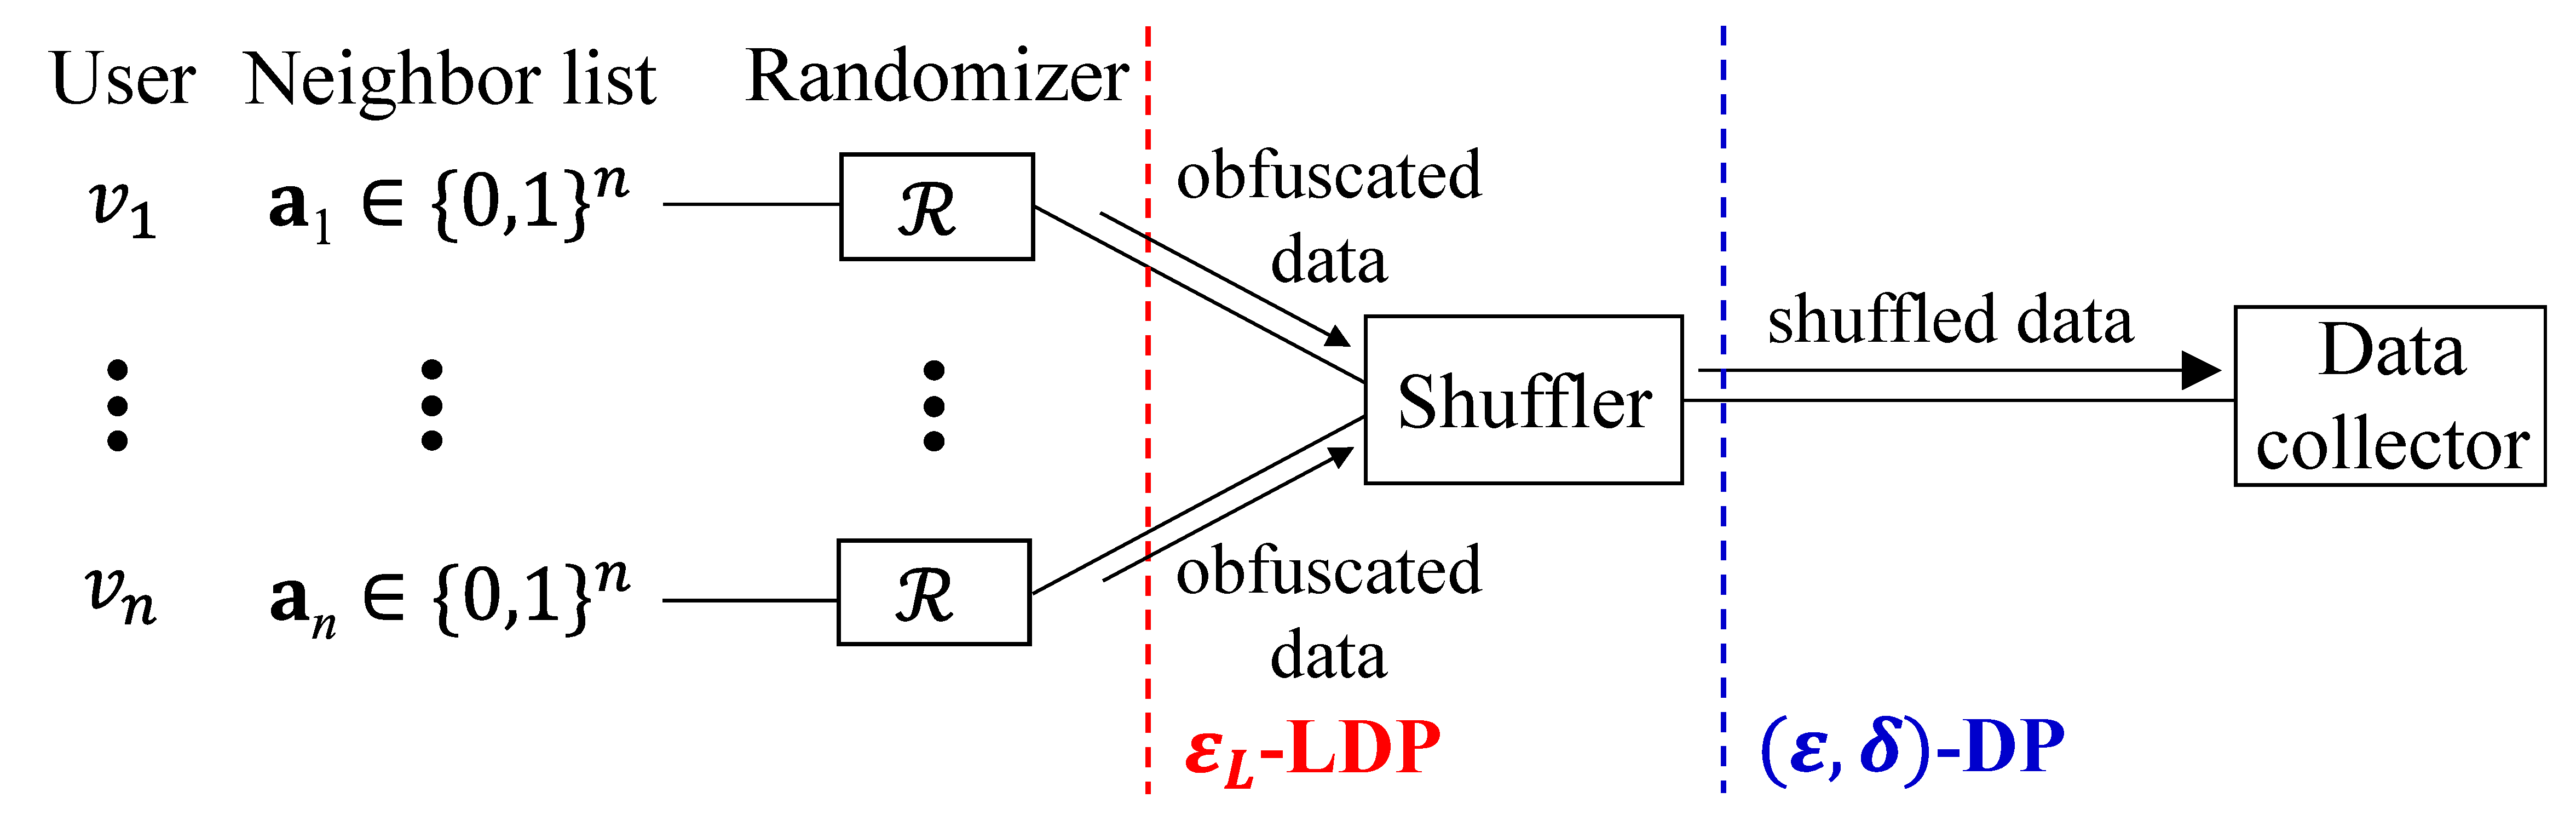
\includegraphics[width=0.99\linewidth]{fig/shuffle.pdf}
%   
%   \caption{Shuffle model. 
%   User $v_i$ obfuscates input data $x_i$ 
%   % calculated from her neighbor list $\bma_i$ 
%   and sends the obfuscated data $y_i$ to the shuffler. 
%   The shuffler sends shuffled data $y_{\pi(1)}, \ldots, y_{\pi(n)}$ to the data collector.
%   }
%   \label{chap3-fig:shuffle_model}
% \end{figure}
% Figure~\ref{chap3-fig:shuffle_model} shows the shuffle model assumed in this paper. 
Thanks to the shuffling, the shuffled data $y_{\pi(1)}, \ldots, y_{\pi(n)}$ available to the data collector provides $(\epsilon, \delta)$-DP, where $\epsilon \ll \epsilon_L$. 

Feldman \textit{et al.} \cite{Feldman_FOCS21} also propose an efficient method to numerically compute a tighter upper bound than the closed-form upper bound in Theorem~\ref{chap3-thm:shuffle}. 
We use both the closed-form and numerical upper bounds in our experiments. 
Specifically, we use the numerical upper bounds in Section~\ref{chap3-sec:experiments} and compare the numerical bound with the closed-form bound in 
\conference{the full version \cite{Imola_CCSFull22}}\arxiv{Appendix~\ref{chap3-sec:numerical_closed}}. 

Assume that $\epsilon$ and $\delta$ in (\ref{chap3-eq:shuffle_epsilon}) are constants. 
Then, by solving for $\epsilon_L$ and changing to big $O$ notation, we obtain  $\epsilon_L = \log(n) + O(1)$. 
This is consistent with the upper bound $\epsilon = O(e^{\epsilon_L / 2} / \sqrt{n})$ in \cite{Feldman_FOCS21}, from which we obtain $\epsilon_L = \log(n) + O(1)$. 
% By (\ref{chap3-eq:shuffle_epsilon}), when we treat $\epsilon$ and $\delta$ as constants, $\epsilon_L$ can be expressed as 
% $\epsilon_L = \log(n) + O(1)$. 
% Similarly, the privacy amplification bounds in \cite{Balle_CRYPTO19,Cheu_EUROCRYPT19} can also be expressed as $\epsilon_L = \Theta(\log(n))$. 
Similarly, the privacy amplification bound in \cite{Cheu_EUROCRYPT19} can also be expressed as $\epsilon_L = \log(n) + O(1)$. 
% This is smaller than other bounds, such as \cite{Balle_CRYPTO19,Erlingsson_SODA19}. 
We use the bound in \cite{Feldman_FOCS21} because it is the state-of-the-art, as described in Section~\ref{chap3-sec:related}. 
% -- it provides smaller $\epsilon$ than other bounds, such as \cite{Balle_CRYPTO19,Cheu_EUROCRYPT19,Erlingsson_SODA19}. 
%and is more general than the bound in \cite{Cheu_EUROCRYPT19} that is specific to binary RR. 
% The bound in \cite{Feldman_FOCS21} also outperforms the bound in \cite{Girgis_CCS21} when it is used without composition, which is the case with this work. 

% Note that the privacy amplification result in \cite{Feldman_FOCS21} assumes that the data elements are shuffled \textit{before} applying the local randomizers, i.e., shuffle-then-randomize. 
% However, 
% shuffling outputs of the same local randomizers (randomize-then-shuffle) 
% is equivalent to first shuffling input data and then applying the local randomizers (shuffle-then-randomize) as described in \cite{Erlingsson_SODA19}. 
% Thus, if all users adopt the same local randomizer, the result in \cite{Feldman_FOCS21} can be applied to the randomize-then-shuffle model, which gives Theorem~\ref{chap3-thm:shuffle}. 

\subsection{Utility Metrics}
\label{chap3-sub:utility}
% Following the existing work, 
We use 
the MSE (Mean Squared Error) 
% the expectation of the $l_2$ loss \cite{Kairouz_ICML16,Murakami_USENIX19,Wang_USENIX17} 
in our theoretical analysis and the relative error 
% \cite{Bindschaedler_SP16,Chen_CCS12,Xiao_SIGMOD11} 
in our experiments. 
The MSE is the expectation of the squared error 
% The $l_2$ loss is a squared error 
between a true value and its estimate. 
Let $f: \calG \rightarrow \nnints$ be a subgraph count function that can be instantiated by $f^\triangle$ or $f^\square$. 
Let $\hf: \calG \rightarrow \reals$ be the corresponding estimator. 
Let 
$\MSE: \reals \rightarrow \nnreals$ be the MSE function, which maps the estimate $\hf(G)$ to the MSE. 
% $l_2^2: \nnints \times \reals \rightarrow \nnreals$ be the expected $l_2$ loss function, which maps the true count $f(G)$ and the estimate $\hf(G)$ to the expected $l_2$ loss. 
Then the MSE can be expressed as $\MSE(\hf(G)) = \E[(f(G) - \hf(G))^2]$, 
% Then it can be expressed as $l_2^2(f(G), \hf(G)) = \E[(f(G) - \hf(G))^2]$, 
where the expectation is taken over the randomness in the estimator $\hf$. 
By the bias-variance decomposition \cite{mlpp}, 
the MSE can be expressed as a summation of the squared bias $(\E[\hf(G)] - f(G))^2$ and the variance $\V[\hf(G)] = \E[(\hf(G) - \E[\hf(G)])]^2$. 
Thus, for an unbiased estimator $\hf$ satisfying $\E[\hf(G)] = f(G)$, the MSE is equal to the variance, i.e., $\MSE(\hf(G)) = \V[\hf(G)]$. 

Although the MSE is suitable for theoretical analysis, it tends to be large when the number $n$ of users is large. 
This is because the true triangle and 4-cycle counts are very large when $n$ is large -- $f^\triangle(G) = O(n d_{max}^2)$ and $f^\square(G) = O(n d_{max}^3)$. 
Therefore, we use the relative error in our experiments. 
The relative error is an absolute error divided by the true value and is given by $\frac{|f^\triangle(G) - \hf^\triangle(G)|}{\min\{f^\triangle(G), \eta\}}$, where $\eta \in \nnreals$ is a small positive value. 
Following the convention \cite{Bindschaedler_SP16,Chen_CCS12,Xiao_SIGMOD11}, we set $\eta = \frac{n}{1000}$. 

When the relative error is well below $1$, the estimate is accurate. 
Note that the absolute error smaller than $1$ would be impossible under DP with meaningful $\epsilon$ (e.g., $\epsilon \leq 1$), as we consider counting queries. 
However, the relative error ($=$ absolute error / true count) much smaller than $1$ is possible under DP with meaningful $\epsilon$. 

\section{Shuffle Model for Graphs}
\label{sec:shuffle}
In this work, we apply the shuffle model to graph data to accurately estimate subgraph counts, such as triangles and 4-cycles. 
Section~\ref{sub:technical} explains our technical motivation. 
% the motivation of our approach. 
In particular, we explain why it is challenging to apply the shuffle model to graph data. 
Section~\ref{sub:wedge_shuffle} proposes a wedge shuffle technique to overcome the technical challenge. 

% \subsection{Technical Challenges}
\subsection{Our Technical Motivation}
\label{sub:technical}

\begin{figure}[t]
  \centering
  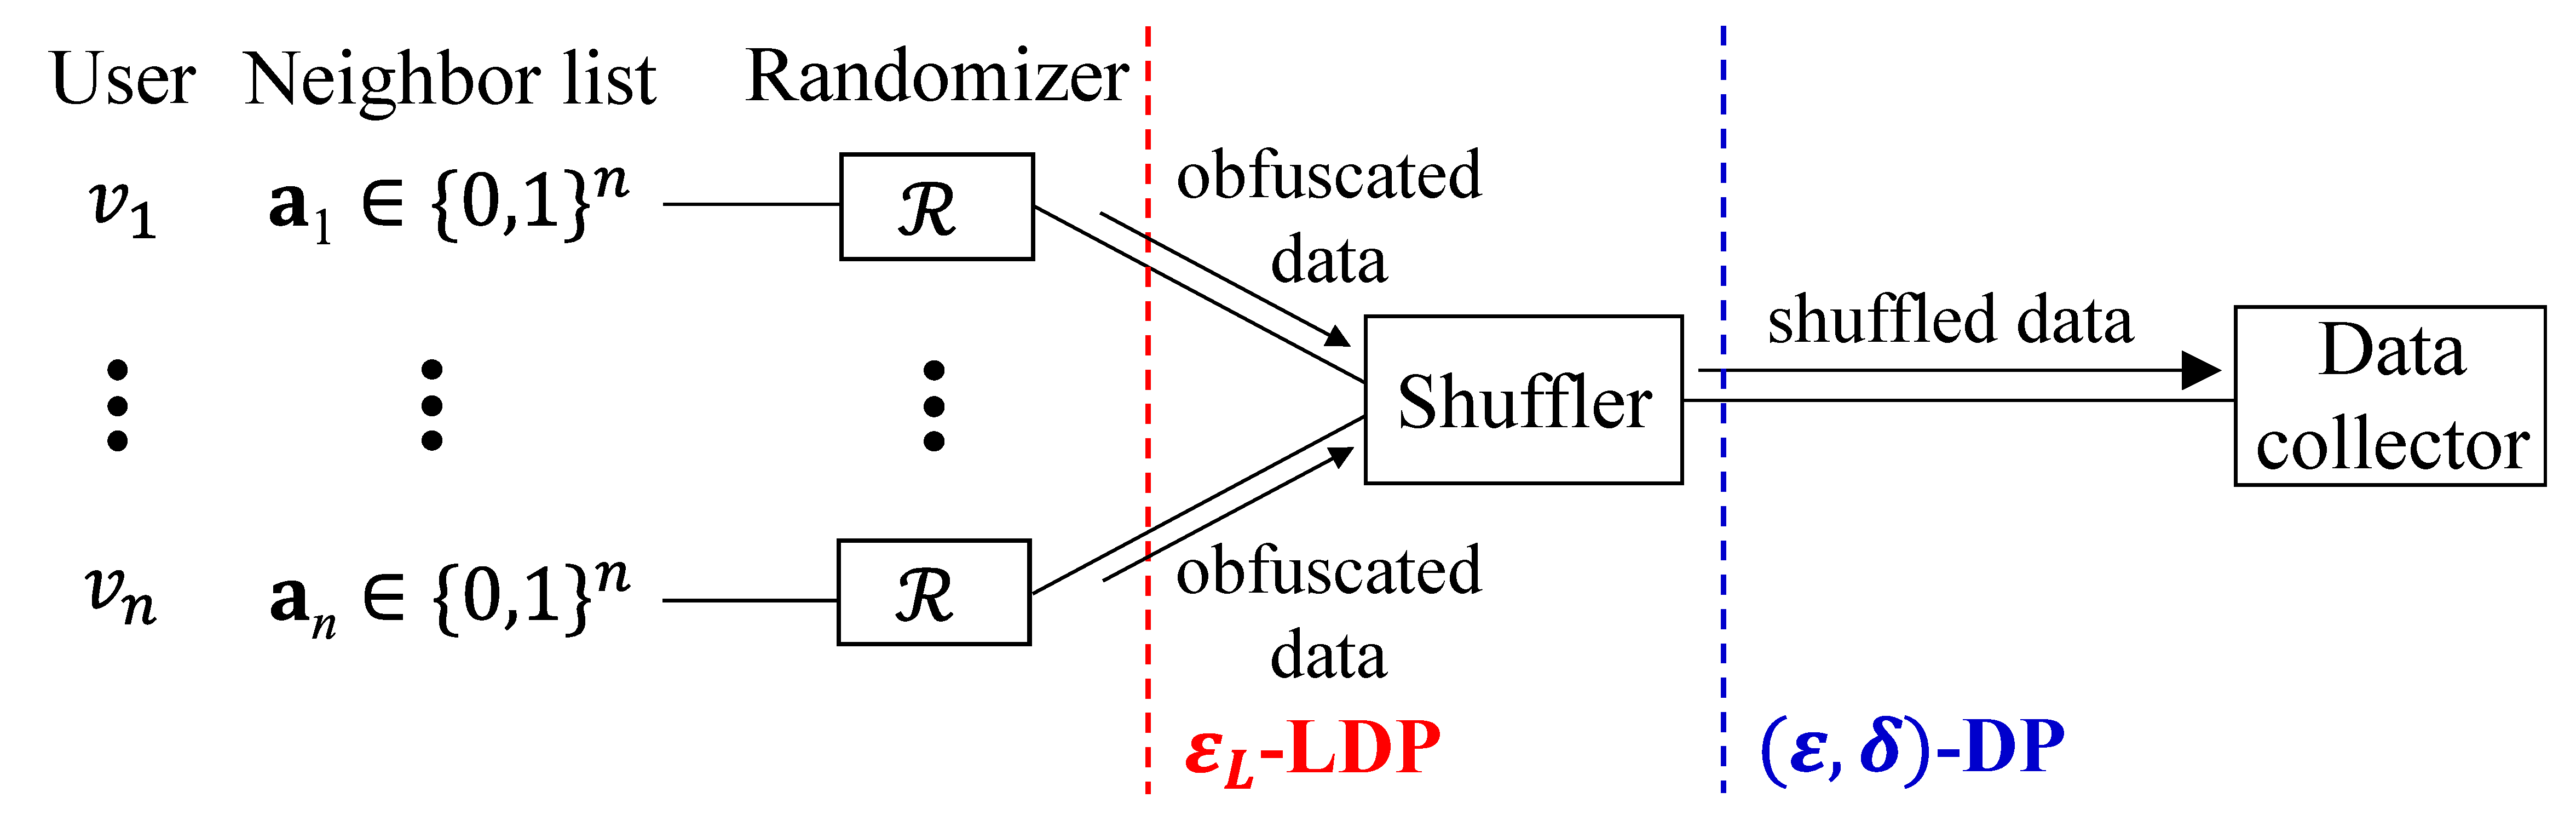
\includegraphics[width=0.99\linewidth]{fig/shuffle.pdf}
  \vspace{-2mm}
  \caption{Shuffle model for graphs. 
  %User $v_i$ calculates input data from her neighbor list $\bma_i$ and obfuscates the input data. 
  %The shuffler randomly shuffles the obfuscated data. 
  }
  \label{fig:shuffle_model}
\end{figure}

% the privacy-utility trade-off can be significantly improved 
% The privacy budget $\epsilon$ (hence the estimation error at the same value of $\epsilon$) can be dramatically reduced by introducing the shuffler. 
The shuffle model has been introduced to dramatically reduce the privacy budget $\epsilon$ (hence the estimation error at the same $\epsilon$) in tabular data \cite{Meehan_ICLR22,Wang_PVLDB20} or 
% image data 
gradients 
\cite{Girgis_AISTATS21,Liu_AAAI21}. 
However, it is very challenging to apply the shuffle model to graph data, 
% analysis, 
as explained below. 

Figure~\ref{fig:shuffle_model} shows the shuffle model for graph data, where each user $v_i$ has her neighbor list $\bma_i \in \{0,1\}^n$. 
% The main reason for this 
The main challenge here 
% in the graph shuffle model 
is that 
% because 
the shuffle model uses a \textit{standard} definition of LDP for the local randomizer and that a neighbor list is \textit{high-dimensional data}, i.e., $n$-dim binary string. 
Specifically, LDP in Definition~\ref{def:LDP} requires any pair of inputs $x$ and $x'$ to be indistinguishable; i.e., 
the inequality (\ref{eq:LDP}) must hold for all pairs of possible inputs. 
Thus, if we use the entire neighbor list 
% (i.e., $n$-dim binary string) 
as input data (i.e., $\bma_i = x_i$ in Theorem~\ref{thm:shuffle}), 
% the standard LDP definition destroys 
either privacy or utility is destroyed for large $n$. 

To illustrate this, consider the following example. 
Assume that $n=10^5$ and $\delta=10^{-8}$. 
Each user $v_i$ applies 
% Warner's RR 
$\epsilon_0$-RR 
with $\epsilon_0=1$ to each bit of her neighbor list $\bma_i$. 
This mechanism is called the randomized neighbor list \cite{Qin_CCS17} and provides $\epsilon_0$-edge LDP. 
% which considers two neighbor lists that differ in one bit. 
However, the privacy budget $\epsilon_L$ in the standard LDP (Definition~\ref{def:LDP}) 
is extremely large -- by group privacy \cite{DP}, $\epsilon_L = n \epsilon_0 = 10^5$. 
Because 
$\epsilon_L$ 
% $n\epsilon$ 
is much larger than $\log (\frac{n}{16 \log (2/\delta)}) = 8.09$, we cannot use the privacy amplification result in Theorem~\ref{thm:shuffle}. 
This is evident from the fact that the shuffled data $y_{\pi(1)}, \ldots, y_{\pi(n)}$ are easily re-identified when $n$ is large. 
If we use 
% Warner's RR 
$\epsilon_0$-RR 
with $\epsilon_0 = \frac{1}{n}$, we can use the amplification result (as $\epsilon_L = n \epsilon_0 = 1$). 
However, it makes obfuscated data almost a random string and destroys the utility because $\epsilon_0$ is too small. 

In this work, we address this issue by introducing a basic technique, which we call \textit{wedge shuffling}. 

\subsection{Our Approach: Wedge Shuffling}
\label{sub:wedge_shuffle}

% To accurately count subgraphs such as triangles and 4-cycles, we propose a basic technique, which we call \textit{wedge shuffling}. 

% \smallskip
% \noindent{\textbf{Overview.}}~~
Figure ~\ref{fig:wedge_shuffle} shows the overview of our wedge shuffle technique. 
% First, we propose a basic technique, which we call wedge shuffling, to enable privacy amplification of graph data by shuffling. 
This technique calculates the number of wedges (2-hop paths) between 
% a specific user-pair $(v_i, v_j)$. 
a specific pair of users $v_i$ and $v_j$. 
%from user $v_i$ to $v_j$. 

Algorithm~\ref{alg:WShuffle} shows our wedge shuffle algorithm, which we call \AlgWS{}. 
% Specifically, 
% we consider the problem of counting triangles including a specific user-pair $(v_i, v_j)$ 
% and propose a wedge shuffle algorithm to accurately count them. 
Given users $v_i$ and $v_j$, 
% our wedge shuffle algorithm calculates 
each of the remaining users $v_k$ ($k \ne i, j$) 
% \in [n]\setminus\{i,j\}$) 
calculates a \textit{wedge indicator} $w_{i-k-j} = a_{k,i} a_{k,j}$, 
%\in \{0,1\}$, 
which 
takes $1$ if 
%and only if 
a wedge $v_i$-$v_k$-$v_j$ exists and $0$ otherwise (line 2). 
Then, $v_k$ obfuscates $w_{i-k-j}$ using $\epsilon_L$-RR and sends it to the shuffler (line 3). 
The shuffler randomly shuffles the noisy wedges using a random permutation $\pi$ over 
% $[n-2]$ 
% $[n]\setminus\{i,j\}$ 
$I_{-(i,j)}$ ($=[n]\setminus\{i,j\}$) 
to provide $(\epsilon, \delta)$-DP with $\epsilon \ll \epsilon_L$ (line 5). 
Finally, the shuffler sends the shuffled wedges to the data collector (line 6). 
The only information available to the data collector is  the number of wedges from $v_i$ to $v_j$, i.e., 
% the number of 
common friends of $v_i$ and $v_j$. 

Our wedge shuffling has two main features. 
First, 
% Because 
the wedge indicator $w_{i-k-j}$ is \textit{one-dimensional binary data}. 
Therefore, it can be sent with small noise and small $\epsilon$, unlike the $n$-dimensional neighbor list. 
For example, when $n=10^5$, $\delta=10^{-8}$, and $\epsilon=1$, the value of $\epsilon_L$ in (\ref{eq:shuffle_epsilon_f}) and (\ref{eq:shuffle_epsilon}) is $\epsilon_L = 5.44$. In this case, $\epsilon_L$-RR rarely flips $w_{i-k-j}$ -- the flip probability is $0.0043$. 
In other words, the shuffled wedges are almost free of noise. 

\begin{figure}[t]
  \centering
  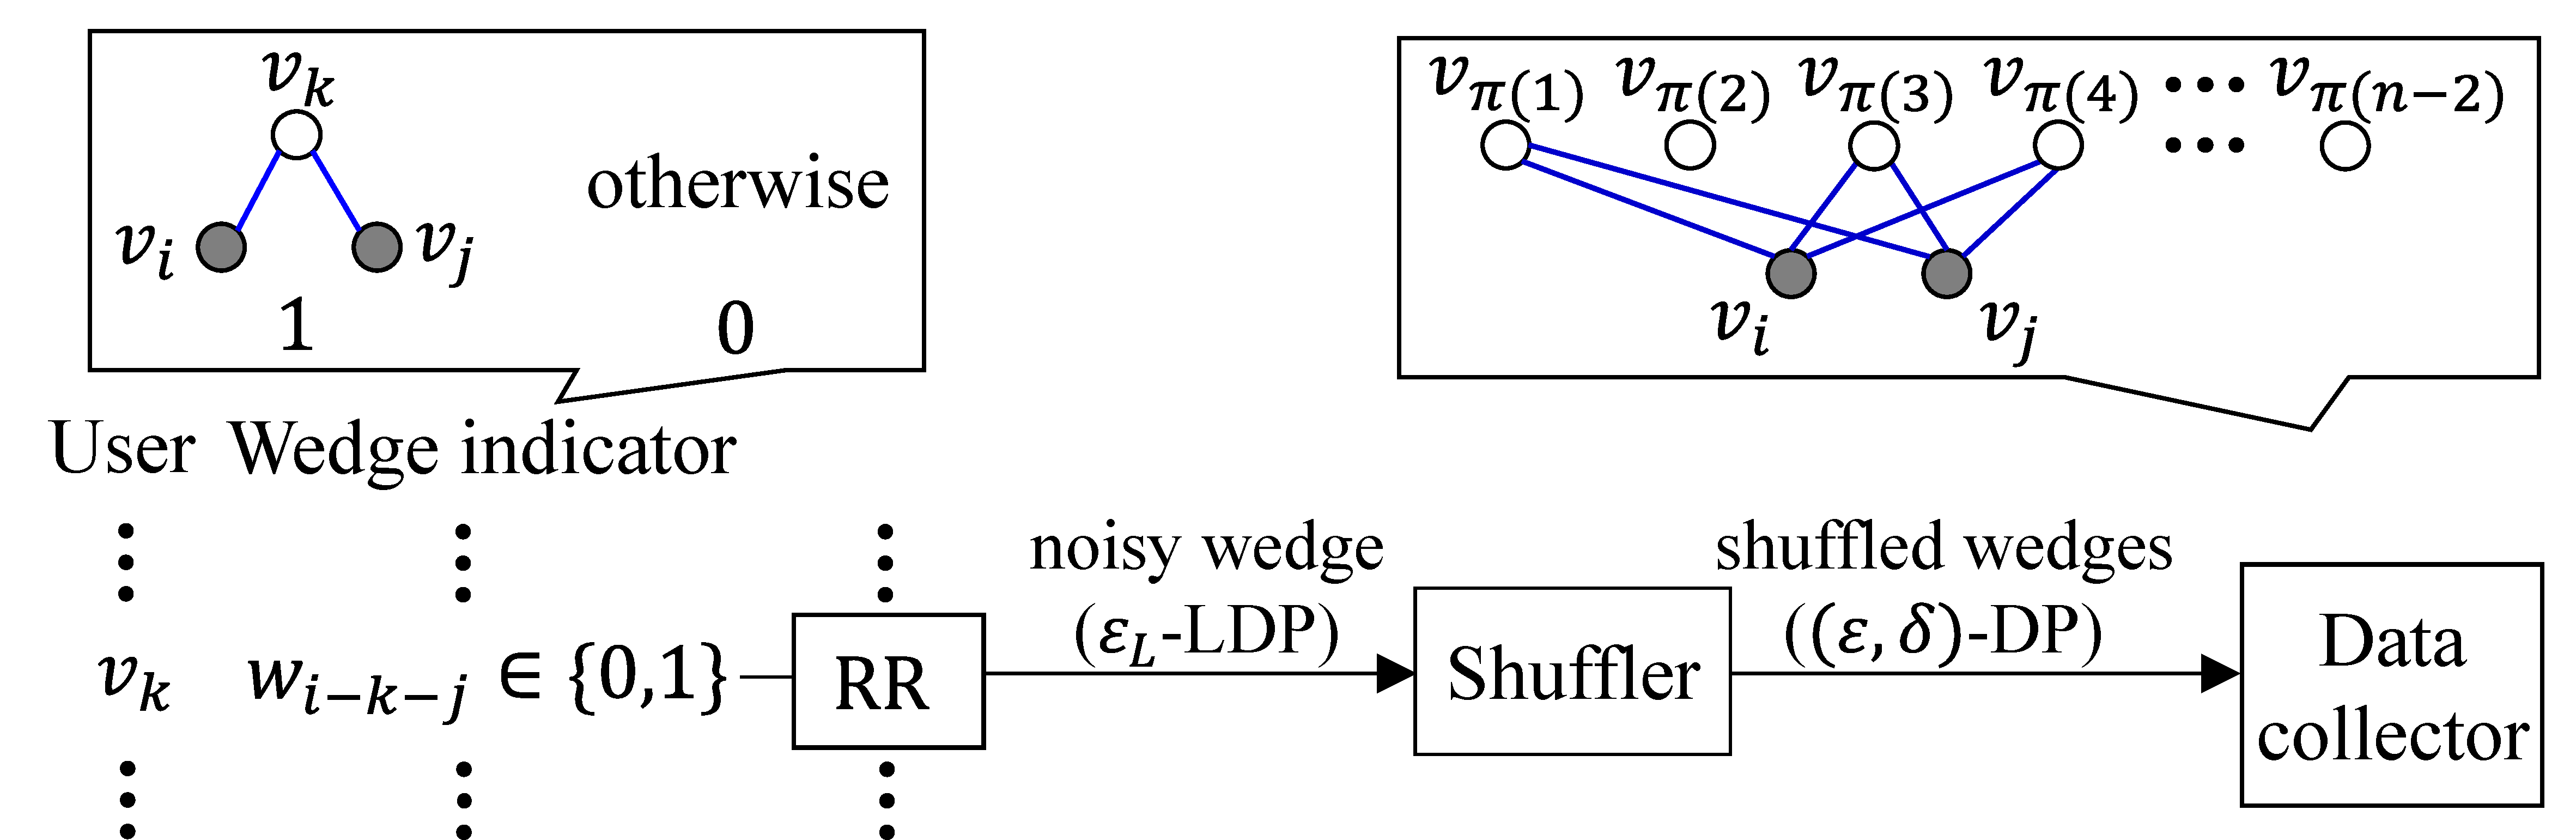
\includegraphics[width=0.99\linewidth]{fig/wedge_shuffle.pdf}
  \vspace{-2mm}
  \caption{Overview of wedge shuffling with inputs $v_i$ and $v_j$. 
  %(marked with gray).
  }
  \label{fig:wedge_shuffle}
\end{figure}

\setlength{\algomargin}{5mm}
\begin{algorithm}[t]
  \SetAlgoLined
  \KwData{Adjacency matrix $\bmA \in \{0,1\}^{n \times n}$, $\epsilon_L \in \nnreals$, user-pair $(v_i,v_j)$.}
  \KwResult{Shuffled wedges $\{y_{\pi(k)} | k \in I_{-(i,j)}\}$.}
%   \tcc{Set-up}
%   $I_{-(i,j)} \leftarrow [n]\setminus\{i,j\}$\;
%   $\epsilon_L \leftarrow \texttt{LocalPrivacyBudget}(n,\epsilon,\delta)$\;
%   \tcc{Users}
  \ForEach{$k \in I_{-(i,j)}$}{
    [$v_k$] $w_{i-k-j} \leftarrow a_{k,i} a_{k,j}$\;
    [$v_k$] $y_k \leftarrow \calR_{\epsilon_L}^W(x)(w_{i-k-j})$; Send $y_k$ to the shuffler\;
  }
%   \tcc{Shuffler}
  [s] Sample a random permutation $\pi$ over $I_{-(i,j)}$\;
  [s] Send $\{y_{\pi(k)} | k \in I_{-(i,j)}\}$ to the data collector\;
%   \tcc{Data collector}
  [d] \KwRet{$\{y_{\pi(k)} | k \in I_{-(i,j)}\}$}
  \caption{Our wedge shuffle algorithm \AlgWS{}. 
  [$v_k$], [s], and [d] represent that the process is run by user $v_i$, the shuffler, and the data collector, respectively. 
  }\label{alg:WShuffle}
\end{algorithm}

Second, the wedge is the main component of many subgraphs such as triangles, 
$k$-triangles \cite{Karwa_PVLDB11}, 
3-hop paths \cite{Sun_CCS19}, 
and 4-cycles. 
For example, a triangle consists of one wedge and one edge, e.g., $v_i-v_{\pi(3)}-v_j$ and $(v_i, v_j)$ in Figure ~\ref{fig:wedge_shuffle}. 
More generally, a $k$-triangle consists of $k$ triangles sharing one edge. 
Thus, it can be decomposed into $k$ wedges and one edge. 
% Similarly, a 
A 3-hop path consists of one wedge and one edge. 
A 4-cycle consists of two wedges, e.g., $v_i-v_{\pi(1)}-v_j$ and $v_i-v_{\pi(3)}-v_j$ in Figure ~\ref{fig:wedge_shuffle}. 
Because the shuffled wedges have little noise, we can accurately count these subgraphs based on wedge shuffling, compared to local algorithms in which all edges are noisy. 
% The other components can be sent from users to the data collector directly (or through the shuffler without shuffling) after adding LDP noise, e.g., by Warner's RR. 
% For example, if the data collector has a noisy edge between $v_i$ and $v_j$, it can count triangles including $(v_i, v_j)$. 
% Similarly, the data collector can count $k$-triangles that consist of $k$ triangles sharing $(v_i, v_j)$. 
% % Because the shuffled wedges have little noise, our wedge shuffling can significantly reduce the DP noise when compared to local algorithms. 
% Moreover, the data collector can count 4-cycles including $v_i$ and $v_j$ (e.g., $v_i-v_{\pi(1)}-v_j-v_{\pi(3)}-v_i$ in Figure ~\ref{fig:wedge_shuffle}) based only on the shuffled wedges. 
% Because the shuffled wedges have little noise, we can accurately count these subgraphs by sampling user-pairs and shuffling wedges. 

In this work, we focus on triangles and 4-cycles and 
present algorithms with upper bounds on the estimation error based on our wedge shuffle technique. 
% use our wedge shuffle technique for accurately counting them. 

% \smallskip
% \noindent{\textbf{Algorithm.}}~~Algorithm~\ref{alg:WShuffle} shows 

% \subsection{Algorithm}
% \label{sub:4cycle_algorithm}
% TBD

% \subsection{Theoretical Analysis}
% \label{sub:4cycle_theoretical}
% TBD

%!TEX root=main.tex
% \section{Differentially Private Triangle Counting under the Shuffle Model}
% \section{Triangle Counting}
\section{Triangle Counting Based on Wedge Shuffling}
\label{sec:triangle}
% The existing one-round local triangle algorithms \cite{Imola_USENIX21,Imola_USENIX22,Ye_ICDE20,Ye_TKDE21} suffer from an extremely large estimation error; e.g., when $\epsilon=1$ in edge DP, the relative error is much larger than $1$ in our experiments.
% To address this issue, we propose a differentially private one-round triangle counting algorithm based on wedge shuffling.
Based on our wedge shuffle technique, we first propose a
% differentially private
one-round triangle counting algorithm.
% in the shuffle model.
%
% Section~\ref{sub:challenges} explains technical challenges in our work.
% In particular, we explain why it is challenging to apply the shuffle model to graph data.
Section~\ref{sub:triangle_overview} describes the overview of our algorithms.
Section~\ref{sub:wedge} proposes an algorithm for counting triangles involving a specific user-pair
% proposes a wedge shuffle technique
as a building block of our triangle counting algorithm.
Section~\ref{sub:triangle} proposes
our triangle counting algorithm.
%an algorithm for counting triangles in the entire graph.
% a one-round triangle counting algorithm based on the wedge shuffling.
Section~\ref{sub:var_red} proposes a technique to significantly reduce the variance in our triangle counting algorithm. 
% by ignoring sparse user-pairs.
Section~\ref{sub:summary} summarizes the performance guarantees of our triangle algorithms. 
% The proofs of all statements in this section are given in Appendix~\ref{sec:triangle_proof}.

% \subsection{Technical Challenges}
% \label{sub:challenges}
% The limitation of the one-round local triangle algorithms is an extremely large estimation error.
% This limitation comes from the fact that all three edges are noisy in any noisy edge the data collector can see, as described in Section~\ref{sec:intro}.

% \subsection{Algorithm Overview}
\subsection{Overview}
\label{sub:triangle_overview}
Our wedge shuffle technique tells the data collector the number of common friends of $v_i$ and $v_j$.
However, this information is not sufficient to count triangles in the entire graph.
% the data collector still cannot count triangles, because she does not know whether $v_i$ and $v_j$ are friends.
% To accurately count triangles based on wedge shuffling,
% under the shuffle model,
Therefore, we introduce
% four
three additional techniques:
% strategies:
% \textit{(i) shuffling wedges},
\textit{(i) sending local edges},
% \textit{wedge shuffling},
% \textit{edge sampling without replacement}.
% \textit{sampling independent edges},
% \textit{sampling independent pairs of nodes}.
\textit{(ii) sampling disjoint user-pairs},
% \textit{independent edge sampling},
and
\textit{(iii) variance reduction by ignoring sparse user-pairs}.
% Our wedge shuffle algorithm uses the first and second strategies, whereas our one-round triangle counting algorithm uses the third and fourth strategies.
% Figures~\ref{fig:local_edges} and \ref{fig:triangle_count} show the overview of our wedge shuffle and triangle counting algorithms, respectively.
% the first two strategies and the third strategy, respectively.
Below, we briefly explain each technique.

\begin{figure}[t]
  \centering
  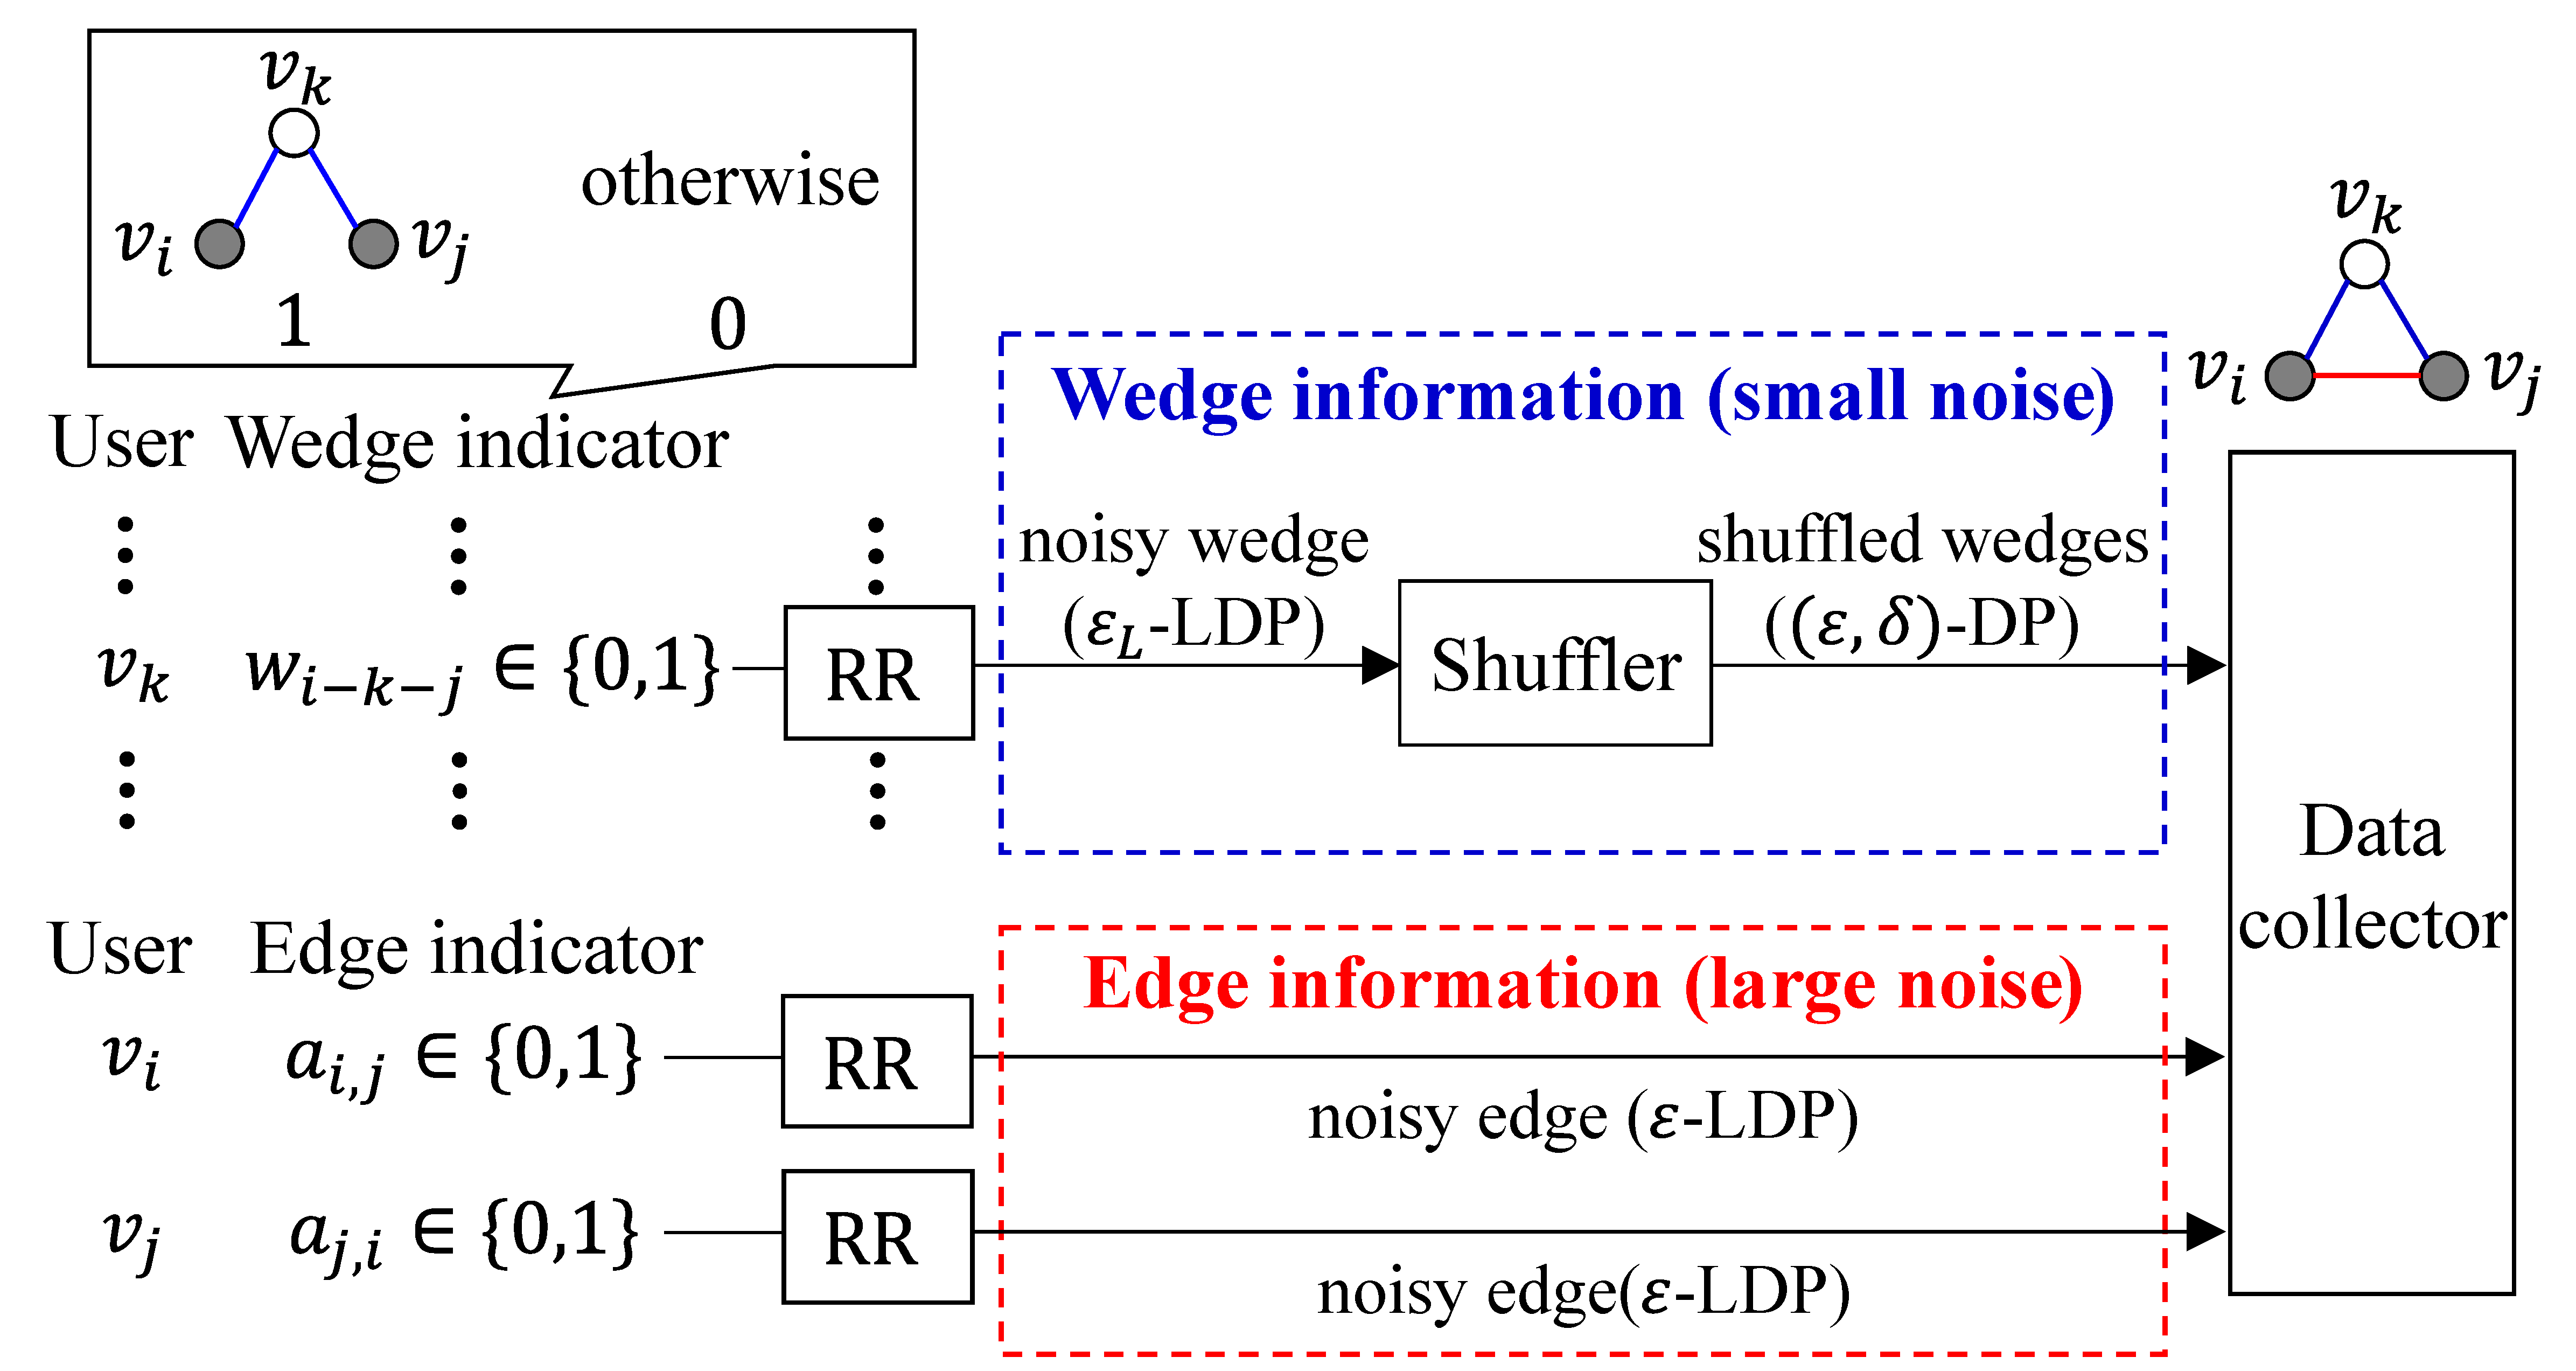
\includegraphics[width=0.99\linewidth]{fig/local_edges.pdf}
  \vspace{-2mm}
  \caption{Overview of our \AlgWSLE{} (Wedge Shuffling with Local Edges) algorithm with inputs $v_i$ and $v_j$.
  %our wedge shuffle algorithm with inputs $v_i$ and $v_j$.
  %(marked with gray).
  }
  \label{fig:local_edges}
% \end{figure}
\vspace{2mm}
% \begin{figure}[t]
  \centering
  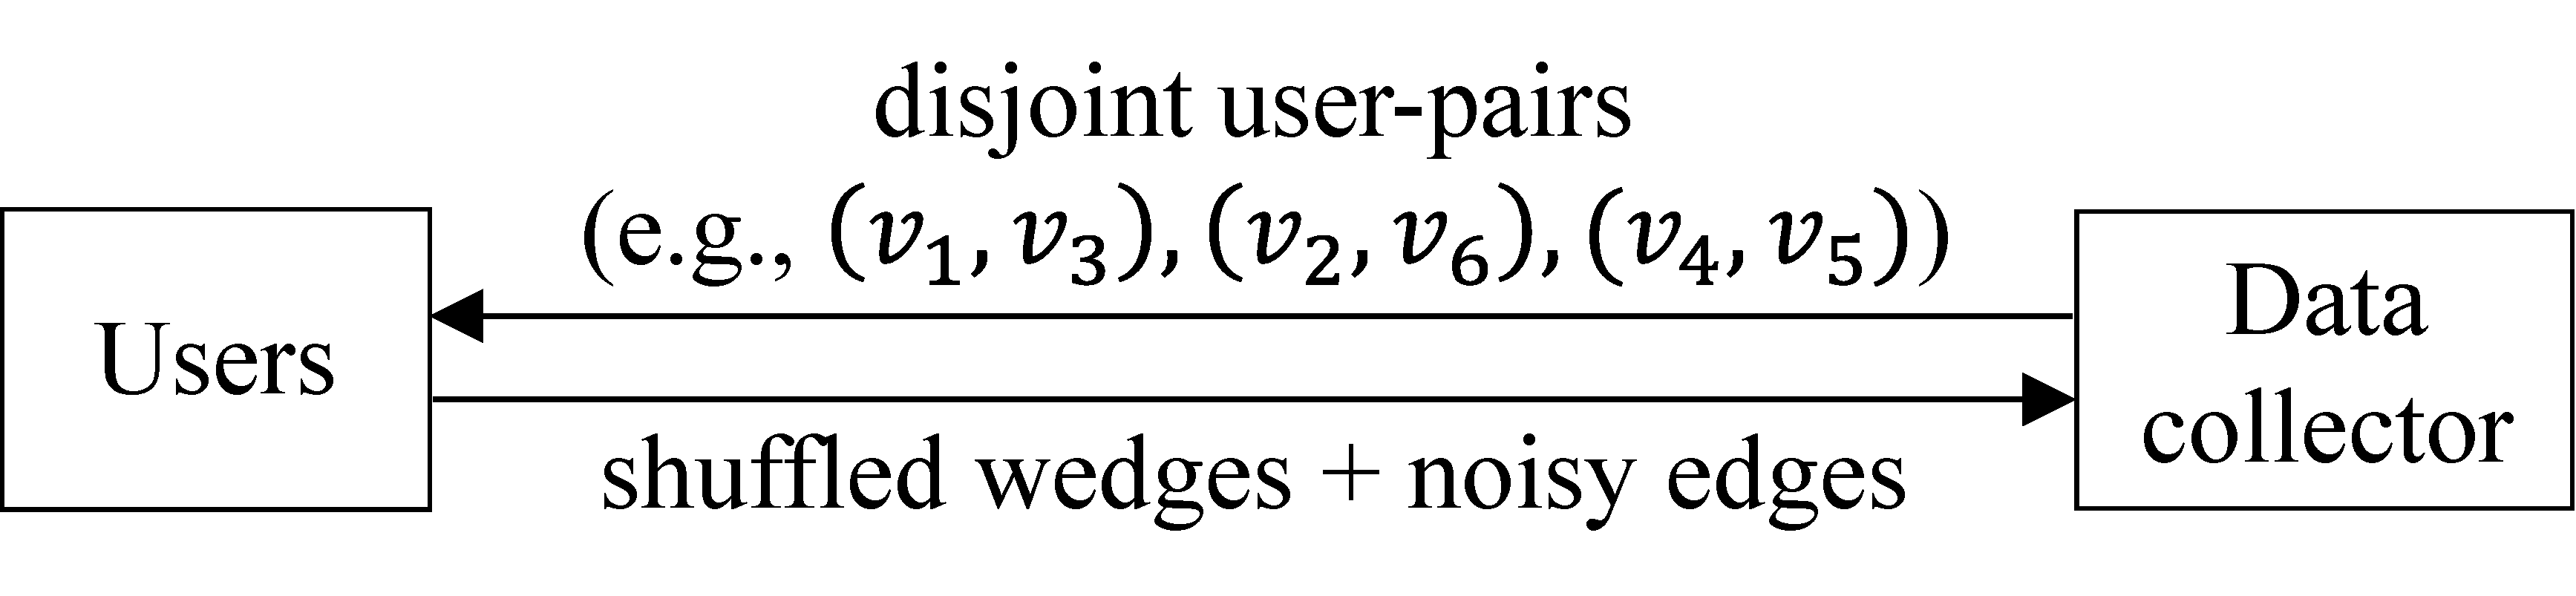
\includegraphics[width=0.7\linewidth]{fig/sampling_pairs2.pdf}
  \vspace{-2mm}
  \caption{Overview of our triangle counting algorithm.
  We use our
  %wedge shuffle
  \AlgWSLE{}
  algorithm with each user-pair.
  %Independent pairs of nodes do share common nodes, e.g., $(v_1, v_3)$, $(v_2, v_6)$, $(v_4, v_5)$.
  }
  \label{fig:triangle_count}
\end{figure}

\smallskip
\noindent{\textbf{Sending Local Edges.}}~~First, we consider the problem of counting triangles involving a specific user-pair $(v_i, v_j)$ and propose an algorithm to send
% The shuffled wedge indicators tell us the number of common friends of $v_i$ and $v_j$.
% However, the data collector still cannot count triangles, because she does not know whether $v_i$ and $v_j$ are friends.
% Thus, our wedge shuffle algorithm sends
\textit{local edges} between $v_i$ and $v_j$, along with shuffled wedges, to the data collector.
We call this the \AlgWSLE{} (Wedge Shuffling with Local Edges) algorithm.
%algorithm \AlgWSLE{} (Wedge Shuffle Edge Local).
% the \textit{wedge shuffling with local edges} algorithm and abbreviate it to \AlgWSLE{}.

Figure~\ref{fig:local_edges} shows the overview of \AlgWSLE{}.
In this algorithm, users $v_i$ and $v_j$ obfuscate edge indicators $a_{i,j}$ and $a_{j,i}$, respectively, using $\epsilon$-RR and send them to the data collector directly (or through the shuffler without shuffling).
%\footnote{It is also possible to send the noisy edge indicators from users $v_i$ and $v_j$ to the data collector through the shuffler. In this case, the shuffler does not shuffle these data.}.
Then, the data collector calculates an unbiased estimate of the triangle count
% from the noisy data.
from the shuffled wedges and the noisy edges.
Because $\epsilon$ is small, a large amount of noise is added to the edge indicators.
However, \textit{only one edge} is noisy (the other two have little noise) in any triangle the data collector sees.
This brings us an advantage over the one-round local algorithms in which all three edges are noisy.

\smallskip
\noindent{\textbf{Sampling Disjoint User-Pairs.}}~~Next, we consider the problem of counting triangles in the entire graph $G$.
A naive solution to this problem is to use our
%wedge shuffling
\AlgWSLE{} algorithm
with all $\binom{n}{2}$ user-pairs as input.
However, it results in very large $\epsilon$ and $\delta$ because it uses each element of the adjacency matrix $\bmA$ many times.
To address this issue,
% To accurately count them under DP,
we propose a triangle counting algorithm that samples
% independent edges (a.k.a. matching), which have no nodes in common.
disjoint user-pairs, ensuring that no user falls in two pairs. 
% which share no common users.
% and then uses the wedge shuffling algorithm for each sampled edge.

Figure~\ref{fig:triangle_count} shows the overview of our triangle algorithm.
The data collector sends the sampled user-pairs to users.
Then, users apply
%our wedge shuffling algorithm
\AlgWSLE{}
with each user-pair
% as input
and send the results to the data collector.
Finally, the data collector calculates an unbiased estimate of the triangle count from the results.
% This can be viewed as edge sampling \cite{Bera_KDD20,Eden_FOCS15,Wu_TKDE16} in triangle counting.
% Edge sampling is known as an efficient sampling method that outperforms other sampling methods such as node sampling and triangle sampling \cite{Wu_TKDE16}.
% Our triangle counting algorithm is also efficient and
% In fact,
Because our triangle algorithm uses each element of
% the adjacency matrix
$\bmA$ \textit{at most once}, it provides $(\epsilon,\delta)$-element DP hence $(2\epsilon,2\delta)$-edge DP.
In addition, our triangle algorithm reduces the time complexity from $O(n^3)$ to $O(n^2)$ by sampling user-pairs rather than using all user-pairs.
% In addition, our wedge shuffle algorithm with a user-pair $(v_i,v_j)$ provides $(\epsilon,\delta)$-DP for each row in the $i$-th and $j$-th columns of the adjacency matrix $\bmA$, and our triangle algorithm samples independent user-pairs.
% Thus, our algorithm provides $(\epsilon,\delta)$-element DP hence $(2\epsilon,2\delta)$-edge DP.

We prove that the MSE of our triangle counting algorithm is
% $O(n^3 d_{max}^2)$.
$O(n^3)$ when we ignore the factor of $d_{max}$.
% when we regard $\epsilon$ and $\delta$ as constants.
When we do not shuffle wedges, the
% expected
MSE is
% $O(n^5)$.
$O(n^4)$.
% This is much smaller than the existing one-round local algorithm with the same time complexity, whose $l_2$ loss is $O(n^5)$, as shown in Section~\ref{sub:upper}.
In addition, the MSE of the existing one-round local algorithm \cite{Imola_USENIX22} with the same time complexity is $O(n^6)$, as proved in
\conference{the full version \cite{Imola_CCSFull22}}\arxiv{
Appendix~\ref{sec:upper}}.
% Section~\ref{sub:upper}.
% Thus, our algorithm has a much smaller estimation error than the local algorithm.
Thus, our
% wedge shuffling
algorithm
provides a dramatic improvement over the local algorithms.

\smallskip
\noindent{\textbf{Variance Reduction.}}~~Although our
% wedge shuffling
algorithm
dramatically
% reduces
improves
the MSE, the factor of $n^3$ may still be large.
Therefore, we propose a variance reduction technique that ignores sparse user-pairs, where either of the two users has a very small degree.
Our basic idea is that the number of triangles involving such a user-pair is very small
% such user-pairs have a very small number of triangles
and can be approximated by $0$.
By ignoring the sparse user-pairs, we can significantly reduce the variance at the cost of introducing a small bias.
We prove that our variance reduction technique reduces the MSE from $O(n^3)$ to $O(n^\gamma)$ where $\gamma\in[2,3)$ and makes one-round triangle counting more accurate.
%accurate one-round triangle counting possible.
% This enables us to accurately count triangles within one round.


% \subsection{Triangle Counting Including a Specific User-Pair}
% \label{sub:triangle_edge}
% \subsection{Wedge Shuffling with Local Edges}
\subsection{WSLE (Wedge Shuffling with Local Edges)}
% \subsection{Sending Local Edges}
\label{sub:wedge}
% Each user $v_k$ ($k \ne i, j$) calculates wedge information $w_{i-k-j} \in \{0,1\}$ that takes $1$ if there is a two-hop path $v_i-v_k-v_j$ and 0 otherwise.
% Then $v_k$ obfuscates $w_{i-k-j}$ using $\epsilon_L$-RR and sends the noisy wedge to the shuffler.
% The shuffler randomly shuffles the noisy wedges to provide $(\epsilon, \delta)$-DP with $\epsilon \ll \epsilon_L$ and sends them to the data collector.
% In addition, users $v_i$ and $v_j$ obfuscate edge information $a_{i,j}$ and $a_{j,i}$, respectively, using $\epsilon$-RR and directly send them to the data collector.

% \smallskip
\noindent{\textbf{Algorithm.}}~~We first
%Consider the problem of counting triangles including a specific user-pair $(v_i,v_j)$.
% To solve this problem, we
propose
% a wedge shuffle algorithm,
the \AlgWSLE{} algorithm
as a building block of our triangle counting algorithm.
\AlgWSLE{} counts
% which estimates the number of
triangles involving a specific user-pair $(v_i,v_j)$.
% We denote this algorithm by \AlgWSLE{}.

Algorithm~\ref{alg:WSLE} shows \AlgWSLE{}.
% This algorithm estimates the number of triangles including a specific user-pair $(v_i,v_j)$.
Let $f_{i,j}^\triangle: \calG \rightarrow \nnints$ be a function that takes $G \in \calG$ as input and outputs the number $f_{i,j}^\triangle(G)$ of triangles involving $(v_i,v_j)$ in $G$.
Let $\hf_{i,j}^\triangle(G) \in \reals$ be an estimate of $f_{i,j}^\triangle(G)$.
% Let $I_{-(i,j)}$ be the set of indices of users other than $v_i$ and $v_j$, i.e., $I_{-(i,j)} = [n]\setminus\{i,j\}$.

\setlength{\algomargin}{5mm}
\begin{algorithm}[t]
  \SetAlgoLined
  \KwData{Adjacency matrix $\bmA \in \{0,1\}^{n \times n}$,
    %Neighbor lists $\bma_1, \ldots, \bma_n \in \{0,1\}^n$,
    %$\epsilon_L \in \nnreals$, $\delta \in [0,1]$, $\epsilon = f(n-2, \epsilon_L, \delta)$,
    $\epsilon \in \nnreals$, $\delta \in [0,1]$,
    user-pair $(v_i,v_j)$.
  }
  \KwResult{Estimate $\hf_{i,j}^\triangle(G)$ of the number $f_{i,j}^\triangle(G)$ of triangles involving $(v_i,v_j)$.}
  %of the count of triangles including $(v_i,v_j)$.}
%   $I_{-(i,j)} \leftarrow [n]\setminus\{i,j\}$\;
%   $q_L \leftarrow \frac{1}{e^{\epsilon_L}+1}$; $q \leftarrow
  %   \frac{1}{e^\epsilon+1}$\;
  $\epsilon_L \leftarrow \texttt{LocalPrivacyBudget}(n,\epsilon,\delta)$\;
%   $\{y_{\pi(k)} | k \in I_{-(i,j)}\} \leftarrow$ \AlgWS{}$(\bmA, \epsilon, \delta, (v_{\sigma(i)}, v_{\sigma(i+1)}))$\;
  \tcc{Wedge shuffling}
  $\{y_{\pi(k)} | k \in I_{-(i,j)}\} \leftarrow$ \AlgWS{}$(\bmA, \epsilon_L, (v_i, v_j))$\;
  \tcc{Send local edges}
%   \For{$i=1$ \KwTo $n$}{
%   \ForEach{$k \in I_{-(i,j)}$}{
%     [$v_k$] $w_{i-k-j} \leftarrow a_{k,i} a_{k,j}$\;
%     [$v_k$] $y_k \leftarrow \calR_{\epsilon_L}^W(x)(w_{i-k-j})$\;
%     [$v_k$] Send $y_k$ to the shuffler\;
%   }
  [$v_i$] $z_i \leftarrow \calR_{\epsilon}^W(x)(a_{i,j})$; Send $z_i$ to the data collector\;
  [$v_j$] $z_j \leftarrow \calR_{\epsilon}^W(x)(a_{j,i})$; Send $z_j$ to the data collector\;
%   \tcc{Shuffler}
%   [s] Sample a random permutation $\pi$ over $I_{-(i,j)}$\;
%   [s] Send $\{y_{\pi(k)} | k \in I_{-(i,j)}\}$ to the data collector\;
  \tcc{Calculate an unbiased estimate}
  [d] $q_L \leftarrow \frac{1}{e^{\epsilon_L}+1}$; $q \leftarrow
  \frac{1}{e^\epsilon+1}$\;
  [d] $\hf_{i,j}^\triangle(G) \leftarrow \frac{(z_i+z_j-2q)\sum_{k \in
  I_{-(i,j)}} (y_{k} - q_L)}{2(1-2q)(1-2q_L)}$\;
  [d] \KwRet{$\hf_{i,j}^\triangle(G)$}
  \caption{\AlgWSLE{}
  %Our wedge shuffle algorithm
  (Wedge Shuffling with Local Edges).
  \AlgWS{} is shown in Algorithm~\ref{alg:WShuffle}.
  %[$v_i$], [s], and [d] represent that the process is run by user $v_i$, the shuffler, and the data collector, respectively.
  % Lines 1 and 2 are run by all parties.
  }\label{alg:WSLE}
\end{algorithm}

% Given $\epsilon$ and $\delta$,
We first call the function \texttt{LocalPrivacyBudget}, which calculates a local privacy budget $\epsilon_L$ from $n$, $\epsilon$, and $\delta$ (line 1).
Specifically, this function calculates $\epsilon_L$
such that $\epsilon$ is a closed-form upper bound (i.e., $\epsilon = f(n-2, \epsilon_L, \delta)$ in (\ref{eq:shuffle_epsilon_f})) or numerical upper bound in the shuffle model with $n-2$ users.
% \cite{Feldman_FOCS21}.
Given $\epsilon_L$, we can easily calculate the closed-form or numerical upper bound $\epsilon$ by (\ref{eq:shuffle_epsilon}) and the open source code in \cite{Feldman_FOCS21}\footnote{\url{https://github.com/apple/ml-shuffling-amplification}.}, respectively.
Thus, we can also easily calculate $\epsilon_L$ from $\epsilon$ by calculating a lookup table for pairs $(\epsilon, \epsilon_L)$ in advance.

Then, we run our wedge shuffle algorithm \AlgWS{} in Algorithm~\ref{alg:WShuffle} (line 2); i.e., each user $v_k \in I_{-(i,j)}$ sends her obfuscated wedge indicator
% obfuscates $w_{i-k-j}$ using $\epsilon_L$-RR $\calR_{\epsilon_L}^W$ and sends the result
$y_k = \calR_{\epsilon_L}^W(w_{i-k-j})$ to the shuffler, and the shuffler sends
shuffled wedge indicators $\{y_{\pi(k)} | k \in I_{-(i,j)}\}$ to the data collector.
%calculates a wedge indicator $w_{i-k-j} \in \{0,1\}$ from her neighbor list $\bma_k$ as follows: $w_{i-k-j} = a_{k,i} a_{k,j}$.
%User $v_k$
% (lines 4-6).
Meanwhile, user $v_i$ obfuscates her edge indicator $a_{i,j}$ using $\epsilon$-RR $\calR_{\epsilon}^W$ and sends the result $z_i = \calR_{\epsilon}^W(a_{i,j})$ to the data collector
% \footnotemark[1]
(line 3).
Similarly, $v_j$ sends $z_j = \calR_{\epsilon}^W(a_{j,i})$ to the data collector (line 4).

% The shuffler samples a uniform random permutation $\pi$ over $I_{-(i,j)}$ and shuffles the wedge indicators based on $\pi$.
% Then, the shuffler sends the shuffled wedge indicators $\{y_{\pi(k)} | k \in I_{-(i,j)}\}$ to the data collector (lines 12-13).

% After receiving $\{y_{\pi(k)} | k \in I_{-(i,j)}\}$, $z_i$, and $z_j$,
Finally, the data collector estimates $f_{i,j}^\triangle(G)$ from $\{y_{\pi(k)} | k \in I_{-(i,j)}\}$, $z_i$, and $z_j$.
% Specifically, let $\hf_{i,j}^\triangle(G) \in \reals$ be an estimate of $f_{i,j}^\triangle(G)$.
Specifically, the data collector calculates the estimate $\hf_{i,j}^\triangle(G)$ as follows:
\begin{align}
    \textstyle{\hf_{i,j}^\triangle(G) = \frac{(z_i+z_j-2q)\sum_{k \in I_{-(i,j)}} (y_{k} -
    q_L)}{2(1-2q)(1-2q_L)},}
    \label{eq:hfij_triangle}
\end{align}
where $q_L = \frac{1}{e^{\epsilon_L}+1}$ and $q = \frac{1}{e^\epsilon+1}$ (lines 5-6).
Note that this estimate involves simply summing over the set $\{y_{\pi(k)}\}$ and does not require knowing the value of $\pi$. This is
consistent with the shuffle model.
As we prove later, $\hf_{i,j}^\triangle(G)$ in (\ref{eq:hfij_triangle}) is an unbiased estimate of $f_{i,j}^\triangle(G)$.

\smallskip
\noindent{\textbf{Theoretical Properties.}}~~Below, we show some theoretical properties of \AlgWSLE{}.
% First, we prove that \AlgWSLE{} provides DP:
% \begin{theorem}
% \label{thm:DP_I}
% \AlgWSLE{} provides $(\epsilon, \delta)$-element DP and $(2\epsilon, 2\delta)$-edge DP.
% \end{theorem}
% Intuitively, Theorem~\ref{thm:DP_I} comes from the fact that \AlgWSLE{} uses only the $i$-th and $j$-th columns of the adjacency matrix $\bmA$ and protects each element with $(\epsilon,\delta)$-DP.
% See Appendix~\ref{sec:triangle_proof} for details.
%
% Next,
First, we prove that
the estimate $\hf_{i,j}^\triangle(G)$
% of \AlgWSLE{}
is unbiased:
\begin{theorem}
\label{thm:unbiased_I}
  For any indices $i,j \in [n]$, the estimate produced by
  $\AlgWSLE{}$ satisfies $\E[\hf_{i,j}^\triangle(G)] = f_{i,j}^\triangle(G)$.
% \AlgWSLE{} provides an unbiased estimate, i.e.,
% \begin{align*}
% \E[\hf_{i,j}^\triangle(G)] = f_{i,j}^\triangle(G).
% \end{align*}
\end{theorem}

% Finally,
Next,
we show the MSE ($=$ variance). 
% of \AlgWSLE{}.
% $\hf_{i,j}^\triangle(G)$.
Recall that in the shuffle model, $\epsilon_L = \log n + O(1)$ when $\epsilon$ and $\delta$ are constants.
%see Section~\ref{sub:shuffle}
We show
% the expected $l_2$ losses for a general case and the case where $\epsilon_L = \Theta(\log n)$:
the MSE for a general case and for the shuffle model:
\begin{theorem}
\label{thm:l2-loss_I}
  For any indices $i,j \in [n]$, the estimate produced by
  \AlgWSLE{} provides the following utility guarantee:
% In \AlgWSLE{},
\begin{align}
& \MSE(\hf_{i,j}^\triangle(G)) = \V[\hf_{i,j}^\triangle(G)] \nonumber\\
  & \leq \frac{n q_L + q(1-2q_L)^2 d_{max}^2}{(1-2q)^2(1-2q_L)^2} \triangleq
  err_{\AlgWSLE}(n,d_{max},q,q_L).
\label{eq:l2_I_general}
\end{align}
  When $\epsilon$ and $\delta$ are constants and $\epsilon_L = \log n + O(1)$, we
  have
\begin{align}
  & err_{\AlgWSLE{}}(n,d_{max}, q, q_L) = O(d_{max}^2).
\label{eq:l2_I_shuffle}
\end{align}
\end{theorem}
The equation (\ref{eq:l2_I_shuffle}) follows from (\ref{eq:l2_I_general}) because $q_L = \frac{1}{e^{\epsilon_L}+1} = \frac{1}{n e^{O(1)} + 1}$. 
% Theorem~\ref{thm:l2-loss_I} states that
Because \AlgWSLE{} is a building block for our triangle counting algorithms, we
introduce the notation $err_{\AlgWSLE{}}(n,d_{max}, q, q_L)$ for our upper bound
in~\eqref{eq:l2_I_general}. Observing
\eqref{eq:l2_I_general}, if we do not use the shuffling technique (i.e.,
$\epsilon_L = \epsilon$), then $err_{\AlgWSLE{}}(n,d_{max}, q, q_L) = O(n + d_{max}^2)$ when we
treat $\epsilon$ and $\delta$ as constants.
In contrast, in the shuffle model where we have $\epsilon_L = \log n + O(1)$,
then $err_{\AlgWSLE{}}(n,d_{max}, q, q_L) = O(d_{max}^2)$.
This means that wedge shuffling reduces the MSE from $O(n + d_{max}^2)$ to $O(d_{max}^2)$, which is significant when $d_{max} \ll n$.

% \subsection{Triangle Counting Based on Wedge Shuffle}
% \subsection{Wedge Shuffle-Based Triangle Counting}
% \subsection{WSLE-Based Triangle Counting}
\subsection{Triangle Counting}
% \subsection{Sampling Independent User-Pairs}
\label{sub:triangle}
\noindent{\textbf{Algorithm.}}~~Based on
%Now, we turn our attention to the problem of counting triangles in the entire graph $G$ and propose a triangle counting algorithm
% Our wedge shuffle algorithm \AlgWSLE{} estimates the number of triangles including a specific user-pair $(v_i,v_j)$.
% Based on
% this,
\AlgWSLE{},
we propose an algorithm that counts triangles in the entire graph $G$.
We denote this algorithm by \AlgWSTri{}, as it applies wedge shuffling to triangle counting.

Algorithm~\ref{alg:wshuffle_triangle} shows \AlgWSTri{}.
First, the data collector samples disjoint user-pairs, 
ensuring that no user falls in two pairs. 
% which share no common users.
Specifically, it calls the function \texttt{RandomPermutation}, which samples a uniform random permutation $\sigma$ over $[n]$ (line 1).
Then, it samples disjoint user-pairs as
$(v_{\sigma(1)}, v_{\sigma(2)}), (v_{\sigma(3)}, v_{\sigma(4)}), \ldots, (v_{\sigma(2t-1)}, \allowbreak v_{\sigma(2t)})$, where $t \in [\lfloor \frac{n}{2} \rfloor]$.
The parameter $t$ represents the number of user-pairs and controls the trade-off between the MSE and the time complexity;
when $t = \lfloor \frac{n}{2} \rfloor$, the MSE is minimized and the time complexity is maximized.
The data collector sends the sampled user-pairs to users (line 2).

\setlength{\algomargin}{5mm}
\begin{algorithm}[t]
  \SetAlgoLined
  \KwData{Adjacency matrix $\bmA \in \{0,1\}^{n \times n}$, $\epsilon \in \nnreals$, $\delta \in [0,1]$, $t \in [\lfloor \frac{n}{2} \rfloor]$.
  }
  \KwResult{Estimate $\hf^\triangle(G)$ of $f^\triangle(G)$.}
%   \tcc{Data collector}
  \tcc{Sample disjoint user-pairs}
  [d] $\sigma \leftarrow$\texttt{RandomPermutation}$(n)$\;
  [d] Send $(v_{\sigma(1)}, v_{\sigma(2)}), \ldots, (v_{\sigma(2t-1)}, v_{\sigma(2t)})$ to users\;
%  \ForEach{$i \in \{1, 3, \ldots, 2t-1\}$}{
%    [$d$] Send $(\sigma(i), \sigma(i+1))$ to users\;
%  }
%   \tcc{Users, shuffler, and data collector}
%   \tcc{Wedge shuffling with local edges}
  \ForEach{$i \in \{1, 3, \ldots, 2t-1\}$}{
    $\hf_{\sigma(i), \sigma(i+1)}^\triangle(G) \leftarrow$ \AlgWSLE{}$(\bmA, \epsilon, \delta, (v_{\sigma(i)}, v_{\sigma(i+1)}))$\;
  }
%   \tcc{Data collector}
  \tcc{Calculate an unbiased estimate}
  [d] $\hf^\triangle(G) \leftarrow \frac{n(n-1)}{6t} \sum_{i=1, 3, \ldots, 2t-1} \hf_{\sigma(i),\sigma(i+1)}^\triangle(G)$\;
  [d] \KwRet{$\hf^\triangle(G)$}
  \caption{Our triangle counting algorithm \AlgWSTri{}.
  %Our wedge shuffle-based triangle counting algorithm \AlgWSTri{}.
  %[d] represents that the process is run by the data collector.
  \AlgWSLE{} is shown in Algorithm~\ref{alg:WSLE}.
  }\label{alg:wshuffle_triangle}
\end{algorithm}

Then, we run our wedge algorithm \AlgWSLE{} in Algorithm~\ref{alg:WSLE} with each sampled user-pair as input (lines 3-5).
Finally, the data collector estimates the triangle count $f^\triangle(G)$ as follows:
\begin{align}
    \textstyle{\hf^\triangle(G) = \frac{n(n-1)}{6t} \sum_{i=1, 3, \ldots, 2t-1} \hf_{\sigma(i),\sigma(i+1)}^\triangle(G)}
   \label{eq:hf_triangle_II}
\end{align}
(line 6). 
Note that a single triangle is never counted by more than one user-pair, as the user-pairs never overlap. 
Later, we prove that $\hf^\triangle(G)$ in (\ref{eq:hf_triangle_II}) is unbiased.

\smallskip
\noindent{\textbf{Theoretical Properties.}}~~We prove that
% our triangle counting algorithm
\AlgWSTri{} provides DP:
% Below, we show the privacy and utility of \AlgWSTri{}.
% We first prove that \AlgWSTri{} provides DP:
\begin{theorem}
\label{thm:DP_II}
\AlgWSTri{} provides $(\epsilon, \delta)$-element DP and $(2\epsilon, 2\delta)$-edge DP.
\end{theorem}
Theorem~\ref{thm:DP_II} comes from the fact that
\AlgWSLE{} with a user-pair $(v_i,v_j)$ provides $(\epsilon,\delta)$-DP for each element in the $i$-th and $j$-th columns of the adjacency matrix $\bmA$ and that \AlgWSTri{} samples disjoint user-pairs, i.e., it uses each element of $\bmA$ at most once.
% and protect each element with $(\epsilon,\delta)$-DP.

Note that running \AlgWSLE{} with all $\binom{n}{2}$ user-pairs 
% requires a very large privacy budget --
% By composition,
% it 
provides $((n-2) \epsilon, (n-2) \delta)$-DP, as it uses each element of $\bmA$ at most $n-2$ times.
The privacy budget is very large, even using the advanced composition \cite{DP,Kairouz_ICML15}.
We avoid this issue by sampling user-pairs that share no common users.

We also prove that
% the estimate of \AlgWSTri{} is unbiased:
\AlgWSTri{} provides an unbiased estimate:
% Next, we show the utility of \AlgWSTri{}:
\begin{theorem}
\label{thm:unbiased_II}
The estimate produced by \AlgWSTri{} satisfies $\allowbreak \E[\hf^\triangle(G)] = f^\triangle(G)$.
% \AlgWSTri{} provides an unbiased estimate, i.e.,
% \begin{align*}
% \E[\hf^\triangle(G)] = f^\triangle(G).
% \end{align*}
\end{theorem}

Next, we analyze the MSE ($=$ variance) of \AlgWSTri{}.
This analysis is 
% complicated 
non-trivial 
because \AlgWSTri{} samples each user-pair \textit{without replacement}.
In this case, the sampled user-pairs are not independent.
However, we can prove that
$t$ estimates in (\ref{eq:hf_triangle_II}) are negatively correlated with each other (\conference{see the full version \cite{Imola_CCSFull22} for details}\arxiv{Lemma~\ref{lem:sampling_replacement_var} in Appendix~\ref{sub:l2-loss_II_proof}}).
%the covariance of two estimates $\hf_{\sigma(i),\sigma(i+1)}^\triangle(G)$ and $\hf_{\sigma(j),\sigma(j+1)}^\triangle(G)$ in (\ref{eq:hf_triangle_II})
Thus, the variance of the sum of $t$ estimates
%$\sum_{i=1, 3, \ldots, 2t-1} \hf_{\sigma(i),\sigma(i+1)}^\triangle(G)$
in (\ref{eq:hf_triangle_II}) is upper bounded by the sum of their variances, each of which is given by Theorem~\ref{thm:l2-loss_I}.
This brings us to the following result:

\begin{theorem}
\label{thm:l2-loss_II}
The estimate produced by \AlgWSTri{} provides the following utility guarantee:
\begin{align}
& \MSE(\hf^\triangle(G)) = \V[\hf^\triangle(G)] \nonumber\\
  &\leq
  \frac{n^4}{36t}err_{\AlgWSLE{}}(n,d_{max},q,q_L) +
  \frac{n^3}{36t}d_{max}^3, \label{eq:thm:l2_II}
\end{align}
where $err_{\AlgWSLE{}}(n,d_{max},q,q_L)$ is given by (\ref{eq:l2_I_general}).
  When $\epsilon$ and $\delta$ are constants,  $\epsilon_L = \log(n) + O(1)$, and
  $t = \lfloor\frac{n}{2}\rfloor$, we have
\begin{align}
\MSE(\hf^\triangle(G))
  &\leq
  O(n^3d_{max}^2). \label{eq:thm:l2_II_simp}
\end{align}
\end{theorem}
% Theorem~\ref{thm:unbiased_II} states that the estimate of \AlgWSTri{} is unbiased.

The inequality (\ref{eq:thm:l2_II_simp}) follows from (\ref{eq:l2_I_shuffle}) and (\ref{eq:thm:l2_II}). 
The first and second terms in~(\ref{eq:thm:l2_II}) are caused by
% the randomness in
Warner's RR
% for local edges
and the sampling of disjoint user-pairs, respectively.
In other words, the MSE of \AlgWSTri{} can be decomposed into two factors: the RR
% for local edges
and user-pair sampling.

For example, assume that $t = \lfloor \frac{n}{2} \rfloor$.
When we do not shuffle wedges (i.e., $\epsilon_L = \epsilon$), then
$err_{\AlgWSLE{}}(n,d_{max},q,q_L) = O(n + d_{max}^2)$, and
MSE in (\ref{eq:thm:l2_II}) is $O(n^4 + n^3 d_{max}^2)$.
When we shuffle wedges, the MSE is $O(n^3 d_{max}^2)$.
Thus, when we ignore the factor of $d_{max}$, our wedge shuffle technique reduces the MSE from $O(n^4)$ to $O(n^3)$ in triangle counting.
The factor of $n^3$ is caused by the RR for local edges.
This is intuitive because a large amount of noise is added to the local edges.

Finally, we analyze the time complexity of \AlgWSTri{}.
The time complexity of running \AlgWSLE{} with all $\binom{n}{2}$ user-pairs is $O(n^3)$, as there are $O(n^2)$ user-pairs in total and \AlgWSLE{} requires the time complexity of $O(n)$.
In contrast, the time complexity of \AlgWSTri{} with $t = \lfloor \frac{n}{2} \rfloor$ is $O(n^2)$ because it samples $O(n)$ user-pairs.
Thus, \AlgWSTri{} reduces the time complexity from $O(n^3)$ to $O(n^2)$ by user-pair sampling.
We can further reduce the time complexity at the cost of increasing the MSE by setting $t$ small,
% the number $t$ of sampled user-pairs small,
i.e., $t \ll \lfloor \frac{n}{2} \rfloor$.
% However, it comes at the cost of increasing the $l_2$ loss.

% \subsection{Variance Reduction Based on Ignoring Sparse User-Pairs}
\subsection{Variance Reduction}
\label{sub:var_red}
\noindent{\textbf{Algorithm.}}~~\AlgWSTri{}
% Our triangle counting algorithm \AlgWSTri{}
achieves the MSE of $O(n^3)$ when we ignore the factor of $d_{max}$.
% However, the factor of $n^3$ is still large because the square of the true count $f^\triangle(G)$ is $O(n^2)$.
% To provide a small relative error, we want to reduce the $l_2$ loss of \AlgWSTri{} from $O(n^3)$ to at most $O(n^2)$.
% To this end,
To provide a smaller estimation error,
we propose a variance reduction technique that ignores sparse user-pairs.
We denote our triangle counting algorithm with the variance reduction technique by \AlgWSTriVR{}.

% Let $d_{i,j} = \min\{d_i, d_j\}$ be the minimum degree of users $v_i$ and $v_j$.
As explained in Section~\ref{sub:triangle}, the factor of $n^3$ is caused by the RR for local edges.
However, most user-pairs $v_i$ and $v_j$ have a very small minimum degree
% $d_{i,j} \ll d_{max}$,
$\min\{d_i, d_j\} \ll d_{max}$,
and there is no edge $(v_i, v_j)$ between them in almost all cases.
In addition, even if there is an edge $(v_i, v_j)$, the number of triangles involving the sparse user-pair is very small
% (at most $d_{i,j}-1$)
(at most $\min\{d_i, d_j\}$)
and can be approximated by $0$.
% Thus,
% we can approximate the number of triangles including the sparse user-pair by $0$.
By ignoring such sparse user-pairs, we can dramatically reduce the variance of the RR for local edges at the cost of a small bias.
This is an intuition behind our variance reduction technique.

% Specifically, we consider the following improvement of \AlgWSTri{}.
% Let $d_{i,j} = \min\{d_i, d_j\}$ be the minimum degree of users $v_i$ and $v_j$.
% Below, we assume that the data collector knows each user $v_i$'s degree $d_i$ for ease of explanation.
% Note that $d_i$ can leak the information about edges of $v_i$.
% Thus, we explain how to privately estimate $d_i$ with edge DP within one-round at the end of Section~\ref{sub:var_red}.
Algorithm~\ref{alg:wshuffle_triangle_vr} shows \AlgWSTriVR{}.
This algorithm detects sparse user-pairs based on the degree information.
However, user $v_i$'s degree $d_i$ can leak the information about edges of $v_i$.
Thus, \AlgWSTriVR{} calculates a differentially private estimate of $d_i$ within one round.

\setlength{\algomargin}{5mm}
\begin{algorithm}[t]
  \SetAlgoLined
  \KwData{Adjacency matrix $\bmA \in \{0,1\}^{n \times n}$, $\epsilon_1, \epsilon_2 \in \nnreals$, $\delta \in [0,1]$, $t \in [\lfloor \frac{n}{2} \rfloor]$, $c \in \nnreals$.
  }
  \KwResult{Estimate $\hf^\triangle(G)$ of $f^\triangle(G)$.}
%   \tcc{Data collector}
  \tcc{Sample disjoint user-pairs}
  [d] $\sigma \leftarrow$\texttt{RandomPermutation}$(n)$\;
  [d] Send $(v_{\sigma(1)}, v_{\sigma(2)}), \ldots, (v_{\sigma(2t-1)}, v_{\sigma(2t)})$ to users\;
%   \tcc{Users, shuffler, and data collector}
%   \tcc{Wedge shuffling with local edges}
  \ForEach{$i \in \{1, 3, \ldots, 2t-1\}$}{
    $\hf_{\sigma(i), \sigma(i+1)}^\triangle(G) \leftarrow$ \AlgWSLE{}$(\bmA, \epsilon_2, \delta, (v_{\sigma(i)}, v_{\sigma(i+1)}))$\;
  }
%   \tcc{Users}
  \tcc{Send noisy degrees}
  \For{$i=1$ \KwTo $n$}{
    [$v_i$] $\td_i \leftarrow d_i + \Lap(\frac{1}{\epsilon_1})$; Send $\td_i$ to the data collector\;
  }
%   \tcc{Data collector}
  \tcc{Calculate a variance-reduced estimate}
%   [d] $d_{th} \leftarrow \frac{c}{n} \sum_{i=1}^n \td_i$\;
  [d] $\td_{avg} \leftarrow \frac{1}{n} \sum_{i=1}^n \td_i$; $d_{th} \leftarrow c \td_{avg}$\;
  [d] $D \leftarrow \{i | i = 1, 3, \ldots, 2t-1,
  \min\{\td_{\sigma(i)}, \td_{\sigma(i+1)}\} > d_{th}\}$\;
  [d] $\hf^\triangle(G) \leftarrow \frac{n(n-1)}{6t} \sum_{i \in D} \hf_{\sigma(i),\sigma(i+1)}^\triangle(G)$\;
  [d] \KwRet{$\hf^\triangle(G)$}
  \caption{Our triangle counting algorithm with variance reduction \AlgWSTriVR{}.
  %[$v_i$] and [d] represent that the process is run by user $v_i$ and the data collector, respectively.
  \AlgWSLE{} is shown in Algorithm~\ref{alg:WSLE}.
  }\label{alg:wshuffle_triangle_vr}
\end{algorithm}

Specifically, \AlgWSTriVR{} uses two privacy budgets: $\epsilon_1, \epsilon_2 \in \nnreals$.
The first budget $\epsilon_1$ is for privately estimating $d_i$, whereas the second budget $\epsilon_2$ is for
\AlgWSLE{}.
% wedge shuffling.
Lines 1 to 5 in Algorithm~\ref{alg:wshuffle_triangle_vr} are the same as those in Algorithm~\ref{alg:wshuffle_triangle}, except that Algorithm~\ref{alg:wshuffle_triangle_vr} uses $\epsilon_2$
% rather than $\epsilon$.
to provide $(\epsilon_2, \delta)$-element DP.
After these processes, each user $v_i$ adds the Laplacian noise $\Lap(\frac{1}{\epsilon_1})$ with mean $0$ and scale $\frac{1}{\epsilon_1}$ to her degree $d_i$ and sends the noisy degree $\td_i$ ($= d_i + \Lap(\frac{1}{\epsilon_1})$) to the data collector (lines 6-8).
% Since adding or removing one element changes $d_i$ by at most $1$
Because the sensitivity \cite{DP} of $d_i$ (the maximum distance of $d_i$ between two neighbor lists that differ in one bit) is $1$, adding $\Lap(\frac{1}{\epsilon_1})$ to $d_i$ provides $\epsilon_1$-element DP.

Then, the data collector estimates the average degree $d_{avg}$ as $\td_{avg} = \frac{1}{n}\sum_{i=1}^n \td_i$ and sets a threshold $d_{th}$ of the minimum degree to $d_{th} = c \td_{avg}$, where $c \in \nnreals$ is a small positive number, e.g.,
% $c=1$ or $2$
$c \in [1,10]$ (line 9).
% (line 10).
%$c \in \nnints$ times the private estimate $\frac{1}{n} \sum_{i=1}^n \td_i$ of $d_{avg}$ (line 10).
Finally, the data collector estimates $f^\triangle(G)$ as
%follows:
\begin{align}
    \textstyle{\hf^\triangle(G) = \frac{n(n-1)}{6t} \sum_{i \in D} \hf_{\sigma(i),\sigma(i+1)}^\triangle(G),}
   \label{eq:hf_triangle_II_ast}
\end{align}
where
\begin{align*}
D = \{i | i = 1, 3, \ldots, 2t-1,
  \min\{\td_{\sigma(i)}, \td_{\sigma(i+1)}\} > d_{th}\}
\end{align*}
(lines 10-11).
The difference between (\ref{eq:hf_triangle_II}) and (\ref{eq:hf_triangle_II_ast}) is that (\ref{eq:hf_triangle_II_ast}) ignores sparse user-pairs $v_{\sigma(i)}$ and $v_{\sigma(i+1)}$ such that $\min\{\td_{\sigma(i)}, \td_{\sigma(i+1)}\} \leq d_{th}$.
% Because
Since
$d_{avg} \ll d_{max}$ in practice,
% $\min\{\td_{\sigma(i)}, \td_{\sigma(i+1)}\} \ll d_{max}$
$d_{th} \ll d_{max}$
holds for small $c$.

The parameter $c$ controls the trade-off between the bias and variance of the estimate $\hf^\triangle(G)$.
The larger $c$ is, the more user-pairs are ignored.
Thus, as $c$ increases, the bias is increased, and the variance is reduced.
% Although the optimization of $c$ is challenging and is left for future work,
In practice,
%$c=1$ or $2$
%$c \in [1,10]$
a small $c$ not less than $1$ 
%(e.g., $c \in [1,10]$)
results in a small MSE % for the following reasons.
% First, the bias is small in this case because $c d_{avg} \ll d_{max}$.
% Second,
% Note that
because most real graphs are scale-free networks that have a power-law degree distribution \cite{NetworkScience}.
% where
In the scale-free networks, most users' degrees are smaller than the average degree $d_{avg}$.
For example, in the BA (Barab\'{a}si-Albert) graph model \cite{NetworkScience,Hagberg_SciPy08},
most users' degrees are $\frac{d_{avg}}{2}$.
% with parameter (number of edges per node) $m$, the average degree is $d_{avg} = 2m$ and most users' degrees are $m$.
Thus, if we set
% $c \geq 1$,
%$c=1$ or $2$,
% (e.g., $c=1$ or $2$),
$c \in [1,10]$, for example,
then most user-pairs are ignored (i.e., $|D| \ll t$), which leads to a significant reduction of the variance at the cost of a small bias.
% In our experiments, we set $c=1$.

Recall that the parameter $t$ in \AlgWSTriVR{} controls the trade-off between the MSE and the time complexity. 
Although \AlgWSTriVR{} always samples $t$ disjoint user-pairs, we can modify \AlgWSTriVR{} so that it stops sampling user-pairs right after the estimate $\hf^\triangle(G)$ in (\ref{eq:hf_triangle_II_ast}) is converged. 
We can also sample dense user-pairs $(v_i, v_j)$ with large noisy degrees $\td_i$ and $\td_j$ at the beginning (e.g., by sorting users in descending order of noisy degrees) to improve the MSE for small $t$. 
Evaluating such improved algorithms is left for future work. 

\smallskip
\noindent{\textbf{Theoretical Properties.}}~~As with \AlgWSTri{},
\AlgWSTriVR{} provides the following privacy guarantee:
%\AlgWSTriVR{} also provides DP:

\begin{theorem}
\label{thm:DP_II_ast}
\AlgWSTriVR{} provides $(\epsilon_1 + \epsilon_2, \delta)$-element DP and $(2(\epsilon_1 + \epsilon_2), 2\delta)$-edge DP.
\end{theorem}

Next, we analyze the bias of \AlgWSTriVR{}. Here, we assume most users have a small degree 
using parameters $\lambda \in \nnreals$ and $\alpha \in [0,1)$: 
% Under this assumption, we can show that the set $D$ truly consists of vertex
% pairs such that $d_{i} \geq d_{th}$, and that the noisy estimates $\hd_i$ do not
% result in a ``noisy'' $D$ where $d_i \geq d_{th}$ is often not true. We can then control the bias
% by observing that vertices with high degree are not excluded from $D$.
% As explained above, we use the ideas
% that there are not many edges involving users with degree less than $d_{th}$, and
% that ignoring estimates in which one user has such a low degree will only
% discard up to $d_{th}$ triangles.
% For this theorem and the next,
% let
% $\overline{d}_{th} = cd_{avg} + \frac{7(c+1)\log n}{\epsilon_1}$ and
% $\underline{d}_{th} = cd_{avg} - \frac{7(c+1)\log n}{\epsilon_1}$.
% The $\log n$ terms arise due to
% adding the Laplacian noise to obtain
% the private degrees $\td_{i}$, and they are much smaller than $c d_{avg}$ in
% most applications.

\begin{theorem}
\label{thm:bias_II_ast}
  Suppose that in $G$, there exist $\lambda \in \nnreals$ and $\alpha \in [0,1)$
  such that at most $n^\alpha$ users have a degree larger than
  $\lambda d_{avg}$. Suppose \AlgWSTriVR{} is run with $c \geq \lambda$.
  Then, the estimator produced by
  \AlgWSTriVR{} provides the following bias guarantee:
\begin{align}
    Bias[\hf^\triangle(G)]
    = |\E[\hf^\triangle(G)] - f^\triangle(G)|
    \leq
    \frac{n c^2 d_{avg}^2}{3} +
    %\frac{1}{3}n(c d_{avg})^2 +
    \frac{4 n^\alpha}{3 \epsilon_1^2}.
    %\frac{1}{3} n^\alpha \left(\frac{2}{\epsilon_1}\right)^2.
    \label{eq:thm:bias_II_ast}
\end{align}
\end{theorem}
% The bias in (\ref{eq:thm:bias_II_ast}) depends on $\lambda$ $\alpha$
The values of $\lambda$ and $\alpha$ depend on the original graph $G$.
In the scale-free networks, $\alpha$ is small for a moderate value of $\lambda$.
For example, in the BA graph with $n=107614$ and $d_{avg}=200$ used in \conference{the full version \cite{Imola_CCSFull22}}\arxiv{Appendix~\ref{sec:BA-graph}}, $\alpha = 0.5$, $0.6$, $0.8$, and $0.9$ when $\lambda = 10.1$, $5.4$, $1.6$, and $0.9$, respectively.
When $c$ and $\epsilon_1$ are constants,
% Since $\alpha \in [0,1]$,
% In Theorem~\ref{thm:bias_II_ast}, the $\log n$ term arises due to the Laplacian noise $\Lap(\frac{1}{\epsilon_1})$ to obtain
% the private degree $\td_{i}$.
% Note that $\log n$ is much smaller than $d_{avg}$ in most graph data, e.g., $(\log n, d_{avg}) = (11.6, \allowbreak 227.4)$ or $(13.7, 127.3)$ in our experiments.
% applications.
% Thus, when $c$ is small (e.g., $c=1$ or $2$),
the bias can be expressed as $O(n d_{avg}^2)$.
% by regarding the parameter $c$ as a constant.
% by ignoring the factor of
% $d_{avg}$ ($\ll d_{max}$).

Finally, we show the variance of \AlgWSTriVR{}. 
This result assumes that $c$ is bigger $(= \frac{(1-\alpha) \log n}{\epsilon_1 d_{avg}})$ than $\lambda$. 
%This is necessary 
We assume this 
because otherwise, many sparse users (with $d_i \leq \lambda d_{avg}$) have a noisy degree $\td_i \geq c \td_{avg}$, causing the set $D$ to
be noisy. In practice, the gap between $c$ and $\lambda$ is small because 
$\log n$ is much smaller than $d_{avg}$. 
% Our theorem will use the value

% $K$, the number of nodes in $G$ with degree greater than
% $\underline{d}_{th}$. In practice, this quantity is much less than $O(n)$

\begin{theorem}
\label{thm:var_II_ast}
  Suppose that in $G$, there exist $\lambda \in \nnreals$ and $\alpha \in [0,1)$
  such that at most $n^\alpha$ users have a degree larger than
  $\lambda d_{avg}$. Suppose \AlgWSTriVR{} is
  run with $c \geq \lambda + \frac{(1-\alpha) \log n}{\epsilon_1 d_{avg}}$.
  Then, the estimator produced by
  \AlgWSTriVR{} provides the following variance guarantee:
\begin{align}
  &\V[\hf^\triangle(G)] \leq \nonumber\\
  &\frac{n^2 d_{max}^4}{9} + \frac{2n^{2+2\alpha}}{9t}err_{\AlgWSLE}(n,d_{max},q,q_L) + \frac{n^{2+\alpha}
  d_{max}^3 }{36t}.
%   &\frac{n^2 d_{max}^4}{9} + \frac{n^{2+2\alpha}}{6t}err_{\AlgWSLE}(n,d_{max},q,q_L) + \frac{n^{2+\alpha}
%   d_{max}^3 }{36t}.
  \label{eq:thm:l2_II_ast}
\end{align}
When $\epsilon_1$, $\epsilon_2$, and $\delta$ are constants,
% $\alpha$ satisfies $\alpha < \frac{1}{2}$, and
$\epsilon_L = \log n + O(1)$, and $t = \lfloor\frac{n}{2}\rfloor$,
% then
\begin{align}
%   \V[\hf_*^\triangle(G)] \leq O(n^2 d_{max}^4).
  \V[\hf^\triangle(G)] \leq O(n^2 d_{max}^4 + n^{1+2\alpha} d_{max}^2).
  \label{eq:thm:l2_II_ast_simp}
\end{align}
\end{theorem}

% \colorB{Finally, we show the variance of \AlgWSTriVR{}.
% For simplicity, we assume that we do not add the Laplacian noise to $d_i$, i.e., $\td_i = d_i$.
% This assumption is fine because $\Lap(\frac{1}{\epsilon_1})$ is very small in practice -- we show that adding $\Lap(\frac{1}{\epsilon_1})$ hardly affects the estimation error in our experiments.
% Under this assumption, we show the variance:}
%
% \begin{theorem}
% \label{thm:var_II_ast_wo_Lap}
% \colorB{The estimate produced by \AlgWSTriVR{} without the Laplacian noise ($\td_i = d_i$ for $i\in[n]$) provides the following variance guarantee:
% \begin{align}
% \V[\hf^\triangle(G)] \leq
%   \frac{|D|n^4}{36t^2}err_{\AlgWSLE{}}(n,d_{max},q,q_L) +
%   \frac{|D|n^3}{36t^2}d_{max}^3, \label{eq:thm:l2_II_ast_wo_Lap}
% \end{align}
% where $err_{\AlgWSLE{}}(n,d_{max},q,q_L)$ is given by (\ref{eq:l2_I_general}).
%   When $\epsilon$ and $\delta$ are constants,  $\epsilon_L = \log(n) + O(1)$, and
%   $t = \lfloor\frac{n}{2}\rfloor$, we have
% \begin{align}
% l_2^2(f^\triangle(G), \hf^\triangle(G))
%   &\leq
%   O(|D|n^2d_{max}^2). \label{eq:thm:l2_II_ast_wo_Lap_simp}
% \end{align}}
% \end{theorem}

% The first term in (\ref{eq:thm:l2_II_ast}) comes from the Laplacian noise $\Lap(\frac{1}{\epsilon_1})$ to obtain
% the private degree $\td_i$.
% The latter two terms are similar to those
% of~\eqref{eq:thm:l2_II}.
% \colorR{In practice, $K$ is much less than $n$}.
% Since $K \ll n$, the second term
% in~\eqref{eq:thm:l2_II_ast_simp} is $O(n)$ (ignoring $d_{max},K$ factors), as
% opposed to $O(n^3)$ which \AlgWSTri{} suffers from.
% $O(n^2 d_{max}^2 (|D| + d_{max}))$.
% Thus, when we ignore the factor of $d_{max}$ and $K$,
% (both of which are much smaller than $n$),
The first\footnote{The first term in (\ref{eq:thm:l2_II_ast}) is actually $\frac{(\sum_{i=1}^n d_i^2)^2}{9}$ and is much smaller than $\frac{n^2 d_{max}^4}{9}$. 
We express it as $O(n^2 d_{max}^4)$ in (\ref{eq:thm:l2_II_ast_simp}) for simplicity. 
See \conference{the full version \cite{Imola_CCSFull22}}\arxiv{Appendix~\ref{sub:var_II_ast_proof}} for details.}, second, and third terms in (\ref{eq:thm:l2_II_ast}) are caused by the randomness in the choice of $D$, the RR, and user-pair sampling, respectively. 
By (\ref{eq:thm:l2_II_ast_simp}), our variance reduction technique reduces the variance from $O(n^3)$ to $O(n^\gamma)$ where $\gamma\in[2,3)$ when we ignore the factor of $d_{max}$.
Because the MSE is the sum of the squared bias and the variance, it is also $O(n^\gamma)$.

The value of $\gamma$ in our bound $O(n^\gamma)$ depends on the parameter $c$ in \AlgWSTriVR{}.
For example, in the BA graph ($n=107614$, $d_{avg} = 200$), $\gamma=2$, $2.2$, $2.6$, and $2.8$ ($\alpha=0.5$, $0.6$, $0.8$, and $0.9$) when $c=10.4$, $5.6$, $1.7$, and $1.0$, respectively, and $\epsilon_1=0.1$.
Thus, the variance decreases with increase in $c$.
However, by (\ref{eq:thm:bias_II_ast}), a larger $c$ results in a larger bias. 
In our experiments, we show that \AlgWSTriVR{} provides a small estimation error when $c=1$ to $4$.
When $c=1$, \AlgWSTriVR{} empirically works well despite a large $\gamma$ because most users' degrees are smaller than $d_{avg}$ in practice, as explained above.
This indicates that our upper bound in (\ref{eq:thm:l2_II_ast_simp}) might not be tight when $c$ is around $1$.
Improving the bound is left for future work.

% our technique reduces the variance from $O(n^3)$ to $O(n^2)$.
% Because the expected $l_2$ loss is the summation of the squared bias and the variance, it can also be expressed as $O(n^2)$.

% \commentT{$K$ can be $n$, e.g., in our experiments using \IMDB{}, $\epsilon_1=0.1$, $n=896308$, $d_{avg}=127.3$, and $c=1$. In this case, $\underline{d}_{th} = 127.3 - 1918.8 < 0$.}

\subsection{Summary}
\label{sub:summary}

Table~\ref{tab:upper_bounds_triangle} summarizes the
performance guarantees
% upper bounds
of one-round triangle algorithms providing edge DP.
Here,
% In \AlgWSTriVR{}, we regard $c$ as a constant (e.g., $c=1$ or $2$) and assume that $d_{th} = O(d_{avg})$.
we consider a variant of \AlgWSTri{} that does not shuffle wedges (i.e., $\epsilon_L = \epsilon$) as a one-round local algorithm.
We call this variant \AlgWLTri{} (Wedge Local).
% We also show \AlgARRTri{} \cite{Imola_USENIX22} and \AlgRRTri{} \cite{Imola_USENIX21} as existing one-round local algorithms.
We also show the variance of \AlgARRTri{} \cite{Imola_USENIX22} and \AlgRRTri{} \cite{Imola_USENIX21}.
The time complexity of \AlgRRTri{} is $O(n^3)$\footnote{Technically speaking, the algorithms of \AlgRRTri{} and
the one-round local algorithms in \cite{Ye_ICDE20,Ye_TKDE21} involve counting the number of triangles in a dense
graph. This can be done in time $O(n^\omega)$, where $\omega \in [2,3)$ and $O(n^\omega)$ is the time required for matrix multiplication. However, these algorithms are of theoretical interest,
and they do not outperform naive matrix multiplication except
for very large matrices~\cite{Alman_2021}. Thus, we assume implementations that use naive matrix multiplication in
$O(n^3)$ time.}, and that
% The time complexity
of \AlgARRTri{} is $O(n^2)$ when we set the sampling probability $p_0 \in [0,1]$ of the ARR to $p_0=O(n^{-1/3})$.
We prove the variance of \AlgARRTri{} in this case and \AlgRRTri{}
% We prove the variance of \AlgARRTri{} \cite{Imola_USENIX22} and \AlgRRTri{} \cite{Imola_USENIX21}
%as existing one-round local algorithms.
in \conference{the full version \cite{Imola_CCSFull22}}\arxiv{Appendix~\ref{sec:upper}}.
We do not show the other one-round local algorithms \cite{Ye_ICDE20,Ye_TKDE21} in Table~\ref{tab:upper_bounds_triangle} for two reasons: (i) they have the time complexity of $O(n^3)$ and suffer from a larger estimation error than \AlgRRTri{} \cite{Imola_USENIX22};
% it is reported in \cite{Imola_USENIX22} that they are outperformed by \AlgRRTri{};
(ii) their upper-bounds on the variance and bias are unclear.

\begin{table}[t]
  \caption{Performance guarantees
  %Upper bounds
  of one-round triangle counting algorithms providing edge DP.
  %``Time'' represents the time complexity.
  $\alpha \in [0,1)$. 
  See also footnote 2 for the variance of \AlgWSTriVR{}.
  %$K \ll n$ in practice.
  }
  \vspace{-4mm}
  \centering
%   \begin{tabular}{|l|c|c|}
%     \hline
%     Algorithm & $l_2$ loss & Time complexity \\ \hline
%     \AlgWSTri{} & $O(n^3 d_{max}^2)$ & $O(n^2)$ \\ \hline
%     \AlgWSTriVR{}{} & $O(n^2 d_{max}^2 + n^2 d_{th}^4)$ & $O(n^2)$ \\ \hline
%     \AlgWLTri{} & $O(n^4 + n^3 d_{max}^2)$ & $O(n^2)$ \\ \hline
%     \AlgARRTri{} & $O(n^5)$ & $O(n^2)$ \\ \hline
%     \AlgRRTri{} & $O(n^4)$ & $O(n^3)$ \\ \hline
%   \end{tabular}
  \begin{tabular}{|l|c|c|c|c|}
    \hline
    Algorithm & \hspace{-0.8mm}Model\hspace{-0.8mm} & Variance & Bias & Time \\ \hline
    % \multirow{2}{*}{\AlgWSTriVR{}} & \multirow{2}{*}{shuffle} & \hspace{-1mm}$O(n^2
    % d_{max}^4 \hspace{-0.5mm}+\hspace{-0.5mm} n^{1+2\alpha} d_{max}^2$\hspace{-1mm} & \multirow{2}{*}{\hspace{-1.5mm}$O(n d_{avg}^2)$\hspace{-1.5mm}} & \multirow{2}{*}{$O(n^2)$}
    % \\ & & $ + n^{1+\alpha} d_{max}^3)$ & & 
    \AlgWSTriVR{} & \hspace{-0.8mm}shuffle\hspace{-0.8mm} & \hspace{-1mm}$O(n^2
    d_{max}^4 \hspace{-0.5mm}+\hspace{-0.5mm} n^{1+2\alpha} d_{max}^2)$\hspace{-1mm} & \hspace{-1.5mm}$O(n d_{avg}^2)$\hspace{-1.5mm} & $O(n^2)$\\
    \hline
    % \AlgWSTriVR{} & shuffle & $O(n^2 d_{max}^2 (d_{max}+|D|))$ & $O(n^2 d_{avg}^4)$ & $O(n^2)$ \\ \hline
    \AlgWSTri{} & \hspace{-0.8mm}shuffle\hspace{-0.8mm} & $O(n^3 d_{max}^2)$ & $0$ & $O(n^2)$ \\ \hline
    \AlgWLTri{} & local & $O(n^4 + n^3 d_{max}^2)$ & $0$ & $O(n^2)$ \\ \hline
    \AlgARRTri{} \cite{Imola_USENIX22} & local & $O(n^6)$ & $0$ & $O(n^2)$ \\ \hline
    \AlgRRTri{} \cite{Imola_USENIX21} & local & $O(n^4)$ & $0$ & $O(n^3)$ \\ \hline
  \end{tabular}
  \label{tab:upper_bounds_triangle}
\end{table}

Table~\ref{tab:upper_bounds_triangle} shows that our \AlgWSTriVR{} dramatically outperforms the three local algorithms -- when we ignore $d_{max}$, the MSE of \AlgWSTriVR{} is 
$O(n^\gamma)$ where $\gamma\in[2,3)$, 
whereas that of the local algorithms is $O(n^4)$ or $O(n^6)$.
We also show this through experiments. 

Note that both \AlgARRTri{} and \AlgRRTri{} provide pure DP ($\delta=0$), whereas our shuffle algorithms provide approximate DP ($\delta > 0$). 
However, it would not make a noticeable difference, as $\delta$ is sufficiently small (e.g., $\delta = 10^{-8} \ll \frac{1}{n}$ in our experiments). 

\smallskip
\noindent{\textbf{Comparison with the Central Model.}}~~Finally, we note that our \AlgWSTriVR{} is worse than algorithms in the central model in terms of the estimation error. 
% Our shuffle algorithms are preferable to algorithms providing central DP in terms of the trust model -- the central model assumes that a single party accesses personal data of all users and therefore has a risk that the entire graph is leaked from the party. 
% However, our shuffle algorithms are worse than central algorithms in terms of the estimation error. 

Specifically, Imola \textit{et al.} \cite{Imola_USENIX21} consider a central algorithm that 
adds the Laplacian noise $\Lap(\frac{d_{max}}{\varepsilon})$ to the true count $f^\triangle(G)$ and 
outputs $f^\triangle(G) + \Lap(\frac{d_{max}}{\epsilon})$\footnote{Here, we assume that $d_{max}$ is publicly available; e.g., $d_{max}=5000$ in Facebook \cite{Facebook_Limit}. 
When $d_{max}$ is not public, the algorithm in \cite{Imola_USENIX21} outputs $f(G) + \Lap(\frac{\td_{max}}{\epsilon})$, where $\td_{max} = \max_{i=1,\ldots,n} \td_i$, i.e., the maximum of noisy degrees.}. 
% outputs $f(G) + \Lap(\frac{\td_{max}}{\epsilon_2})$. 
% where $\td_{max} = \max_{i=1,\ldots,n} \td_i$ and $\td_i = d_i + \Lap(\frac{1}{\epsilon_1})$. 
This central algorithm provides 
$(\epsilon, 0)$-edge DP. 
% $(2\epsilon_1 + \epsilon_2, 0)$-edge DP. 
In addition, the estimate is unbiased, and the variance is $\frac{2d_{max}^2}{\epsilon^2} = O(d_{max}^2)$. 
Thus, the central algorithm provides a much smaller MSE ($=$ variance) than \AlgWSTriVR{}. 

However, our \AlgWSTriVR{} is preferable to central algorithms in terms of the trust model -- the central model assumes that a single party accesses personal data of all users and therefore has a risk that the entire graph is leaked from the party. 
\AlgWSTriVR{} can also be applied to decentralized social networks, as described in Section~\ref{sec:intro}. 

% \subsection{Lower Bounds for Local Algorithms}
% \label{sub:two-rounds}
% TBD

% \subsection{Algorithm}
% \label{sub:triangle_algorithm}
% TBD

% \subsection{Theoretical Analysis}
% \label{sub:triangle_theoretical}
% TBD

% \subsection{4-Cycle Counting}
% \label{sub:4-cycle}
% TBD

%!TEX root=main.tex
\section{4-Cycle Counting Based on Wedge Shuffling}
\label{chap3-sec:4cycle}

Next, we propose a one-round 4-cycle counting algorithm in the shuffle model.
Section~\ref{chap3-sub:4cycle_overview} explains its overview.
Section~\ref{chap3-sub:4cycle_details} proposes our 4-cycle counting algorithm and shows its theoretical properties. 
Section~\ref{chap3-sub:summary_4cycle} summarizes the performance guarantees of our 4-cycle algorithms. 
% The proofs of all statements in this section are given in Appendix~\ref{chap3-sec:4cycle_proof}.

\subsection{Overview}
\label{chap3-sub:4cycle_overview}
% \textbf{Sending Local Wedges}
% To count 4-cycles in the graph based on our wedge shuffling technique, we introduce 
We apply our wedge shuffling technique to 4-cycle counting with two additional techniques: \textit{(i) bias correction} and \textit{(ii) sampling disjoint user-pairs}. 
Below, we briefly explain each of them. 

\smallskip
\noindent{\textbf{Bias Correction.}}~~As with triangles, we begin with the problem of counting 4-cycles involving specific users $v_i$ and $v_j$. 
We can leverage the noisy wedges output by our wedge shuffle algorithm \AlgWS{} to estimate such a 4-cycle count. 
% the number of $4$-cycles
% between two users $v_i, v_j$. 
Specifically, let $f^\square_{i,j}: \calG \rightarrow \nnints$ be a function that, given $G \in \calG$, outputs the number $f^\square_{i,j}(G)$ of $4$-cycles for which users $v_i$ and $v_j$ are opposite nodes, i.e. the number of unordered pairs $(k,k')$ such that $v_i-v_k-v_j-v_{k'}-v_i$ is a path in $G$.
Each pair $(k,k')$ satisfies the above requirement if and only if $v_i-v_k-v_j$ and $v_i-v_{k'}-v_j$ are wedges in $G$.
Thus, we have $f^\square_{i,j}(G) = \binom{f^\wedge_{i,j}}{2}$, where $f^\wedge_{i,j}$ is the number of wedges between $v_i$ and $v_j$. 
Based on this, we calculate an unbiased estimate $\hf^\wedge_{i,j}$ of the wedge count using \AlgWS{}. 
Then, we calculate an estimate of the 4-cycle count as $\binom{\hf^\wedge_{i,j}}{2}$. 
% an unbiased estimate $\hf^\square_{i,j}(G)$ of the 4-cycle count from $\hf^\wedge_{i,j}$. 
Here, it should be noted that the estimate $\binom{\hf^\wedge_{i,j}}{2}$ 
% $\binom{\hf^\wedge_{i,j}}{2}$ 
is \textit{biased}, as proved later. 
%However, $\binom{\hf^\wedge_{i,j}(G)}{2}$ is \textit{not} an unbiased estimate of $f^\square_{i,j}(G)$, as proved later. 
Therefore, 
%Thus, we calculate an unbiased estimate of $f^\square_{i,j}(G)$ via bias correction -- 
we perform bias correction -- we subtract a positive value from the estimate to obtain an unbiased estimate $\hf_{i,j}^\square(G)$ of the 4-cycle count. 

% Because \AlgWS{} can be used to estimate $f^\wedge_{i,j}{2}$, we are able to obtain an estimator $\hf^\square_{i,j}(G)$.
%The estimator is of the form $\binom{\hf^\wedge_{i,j}(G)}{2} - C$, where $C$ is a constant independent of $\hf^\wedge_{i,j}(G)$ that debiases the estimate.
Note that unlike \AlgWSLE{}, no edge between $(v_i,v_j)$ needs to be sent. 
In addition, thanks to the privacy amplification by shuffling, all wedges can be sent with 
% a large $\epsilon$.
small noise.

\smallskip
% \textbf{Sampling Independent User-Pairs} 
\noindent{\textbf{Sampling Disjoint User-Pairs.}}~~Having an estimate $\hf_{i,j}^\square(G)$, we turn our attention to estimating 4-cycle count $f^\square(G)$ in the entire graph $G$.
As with triangles, a naive solution using estimates $\hf_{i,j}^\square(G)$ for all $\binom{n}{2}$ user-pairs $(v_i,v_j)$ results in very large $\epsilon$ and $\delta$. 
To avoid this, we sample disjoint user-pairs and obtain an unbiased estimate of $f^\square(G)$ from them. 
%Naively, we could obtain estimates $\hf_{i,j}^\square(G)$ for all pairs $i,j$, to obtain a concentrated estimate of $\hf^\square(G)$. However, this would not be good for privacy, as each user would send wedge information about all pairs of other vertices, using each value of his adjacency list up to $n$ times. Instead, and identical to the design of \AlgWSTri{}, our algorithm estimates $\hf^\square_{i,j}(G)$ for $t$ disjoint pairs of users with $1 \leq t \leq \lfloor \frac{n}{2} \rfloor$.

\subsection{4-Cycle Counting}
\label{chap3-sub:4cycle_details}

\setlength{\algomargin}{5mm}
\begin{algorithm}[t]
  \SetAlgoLined
  \KwData{Adjacency matrix $\bmA \in \{0,1\}^{n \times n}$, $\epsilon \in \nnreals$, $\delta \in [0,1]$, $t \in [\lfloor \frac{n}{2} \rfloor]$.
  }
  \KwResult{Estimate $\hf^\square(G)$ of $f^\square(G)$.}
  $\epsilon_L \leftarrow \texttt{LocalPrivacyBudget}(n,\epsilon,\delta)$\;
  [d] $q_L \leftarrow \frac{1}{e^{\epsilon_L}+1}$\;
%   \tcc{Data collector}
  \tcc{Sample disjoint user-pairs}
  [d] $\sigma \leftarrow$\texttt{RandomPermutation}$(n)$\;
  [d] Send $(v_{\sigma(1)}, v_{\sigma(2)}), \ldots, (v_{\sigma(2t-1)}, v_{\sigma(2t)})$ to users\;
%  \ForEach{$i \in \{1, 3, \ldots, 2t-1\}$}{
%    [$d$] Send $(\sigma(i), \sigma(i+1))$ to users\;
%  }
%   \tcc{Users, shuffler, and data collector}
%   \tcc{Wedge shuffling}
  \ForEach{$i \in \{1, 3, \ldots, 2t-1\}$}{
    $\{y_{\pi_i(k)} | k \hspace{-1mm}\in I_{-(\sigma(i),\sigma(i+1))}\} \hspace{-1mm}\leftarrow\hspace{-1mm}$ \AlgWS{}$(\bmA, \epsilon_L, (v_{\sigma(i)}, v_{\sigma(i+1)}))$\;
    [d] $\hf_{\sigma(i),\sigma(i+1)}^\wedge(G) \leftarrow \sum_{k \in I_{-(\sigma(i),\sigma(i+1))}} \frac{y_{k} - q_L}{1-2q_L}$\;
    [d] $\hf_{\sigma(i),\sigma(i+1)}^\square(G) \leftarrow  \frac{\hf_{\sigma(i),\sigma(i+1)}^\wedge(G)(\hf_{\sigma(i),\sigma(i+1)}^\wedge(G)-1)}{2} - \frac{n-2}{2}\frac{q_L(1-q_L)}{(1-2q_L)^2}$\;
  }
%   \tcc{Data collector}
  \tcc{Calculate an unbiased estimate}
  [d] $\hf^\square(G) \leftarrow \frac{n(n-1)}{4t}\sum_{i=1,3,\ldots,2t-1} \hf_{\sigma(i),\sigma(i+1)}^\square(G)$\;
  %[d] $\hf^\square(G) \leftarrow \frac{n(n-1)}{4t}\sum_{i=1,3,\ldots,2t-1} \left(\frac{\hf_{\sigma(i),\sigma(i+1)}^\wedge(G)(\hf_{\sigma(i),\sigma(i+1)}^\wedge(G)-1)}{2} - \frac{n-2}{2}\frac{q_L(1-q_L)}{(2q_L-1)^2}\right)$\;
  [d] \KwRet{$\hf^\square(G)$}
  \caption[Our 4-cycle counting algorithm \AlgWSCyc{}.]{Our 4-cycle counting algorithm \AlgWSCyc{}.
  %$\hf^\wedge$ is a shorthand for $\hf_{\sigma(i),\sigma(i+1)}^\wedge(G)$.
  \AlgWS{} is shown in Algorithm~\ref{chap3-alg:WShuffle}.
  }\label{chap3-alg:wshuffle_cycle}
\end{algorithm}

\noindent{\textbf{Algorithm.}}~~Algorithm \ref{chap3-alg:wshuffle_cycle} shows our 4-cycle counting algorithm. 
We denote it by \AlgWSCyc{}. 
% Our algorithm \AlgWSCyc{} produces an unbiased estimator $\hf^\square_{i,j}(G)$. 
% The algorithm appears in Algorithm~\ref{chap3-alg:wshuffle_cycle}. 
First, we set a local privacy budget $\epsilon_L$ from $n$, $\epsilon$, and $\delta$ in the same way as \AlgWSLE{} (line 1). 
%line 1 sets $\epsilon_L$ to be a value such that the entire algorithm in the shuffle model achieves $(\epsilon, \delta)$-DP. This value is given by Theorem~\ref{chap3-thm:shuffle}.
%In lines 3-4, 
Then, we sample $t$ disjoint pairs of users using the permutation $\sigma$ (lines 3-4). 
Each pair is given by $(v_{\sigma(i), \sigma(i+1)})$ for $i \in \{1, 3, \ldots, 2t-1\}$.

%In lines 5-9, 
For each $i \in \{1, 3, \ldots, 2t-1\}$, we compute an unbiased estimate $\hf_{\sigma(i),
\sigma(i+1)}^\square(G)$ of the 4-cycle count involving $v_{\sigma(i)}$ and $v_{\sigma(i+1)}$ (lines 5-9). 
To do this, 
%in line 6 
we call \AlgWS{} on
$(v_{\sigma(i)} v_{\sigma(i+1)})$ to obtain an unbiased estimate $\hf_{\sigma(i),
\sigma(i+1)}^\wedge(G)$ of the wedge count (lines 6-7). 
We calculate an estimate $\hf_{i,j}^\wedge(G)$ of the number $f_{i,j}^\wedge(G)$ of wedges between $v_i$ and $v_j$ in $G$ as follows:
% and is given by
\begin{equation}\label{chap3-eq:wedge-estimate}
  \textstyle{\hf^\wedge_{i,j}(G) = \sum_{k \in I_{-(i,j)}} \frac{y_k - q_L}{1-2q_L}.}
\end{equation}
Later, we will prove that $\hf^\wedge_{i,j}(G)$ is an unbiased estimator. 
As with (\ref{chap3-eq:hfij_triangle}), this estimate involves the sum over the set $\{y_{\pi(k)}\}$ and does not require knowing the permutation $\pi$ produced by the shuffler. 
%Note that each permutation $\pi_i$ used to shuffle the data is distinct for each iteration of the loop, and it is unknown to the data collector.
% In line 8, 
Then, we obtain an unbiased estimator of $f_{\sigma(i), \sigma(i+1)}^\square$ as follows:
%, given by
\begin{equation}\label{chap3-eq:4-cycle-ij-estimate}
  \textstyle{\hf_{i,j}^\square(G) = \frac{\hf^\wedge_{i, j}(G)(\hf^\wedge_{i, j}(G)-1)}{2} - \frac{n-2}{2}\frac{q_L(1-q_L)}{(1-2q_L)^2}}
\end{equation}
(line 8). 
Note that 
% even though 
% $\hf_{i, j}^\wedge(G)$ is unbiased, and we have that $f_{i, j}^\square(G) = \binom{f_{i, j}^\wedge(G)}{2}$, 
% because 
there is a quadratic relationship between $f_{i, j}^\square(G)$ and $f_{i, j}^\wedge(G)$, i.e., $f_{i, j}^\square(G) = \binom{f_{i, j}^\wedge(G)}{2}$. 
% the two quantities, 
Thus, 
even though $\hf_{i, j}^\wedge(G)$ is unbiased, 
we must subtract a term from $\binom{\hf_{i, j}^\wedge(G)}{2}$ (i.e., bias correction) to obtain an unbiased estimator $\hf_{i, j}^\square(G)$. 
This forms the righthand side of
~\eqref{chap3-eq:4-cycle-ij-estimate} and ensures that $\hf_{i,j}^\square(G)$ is unbiased. 
% as we prove later.

Finally, 
%in line 10, 
we sum and scale 
% the sample 
$\hf_{\sigma(i), \sigma(i+1)}^\square(G)$ for each $i$ to obtain an estimate $\hf^\square(G)$ of the 4-cycle count $f^\square(G)$ in the entire graph $G$: 
% is summed and scaled by the proper amount to produce an final estimate:

\begin{equation}\label{chap3-eq:4-cycle-estimate}
  \textstyle{\hf^\square(G) = \frac{n(n-1)}{4t}\sum_{i=1,3,\ldots,2t-1} \hf_{\sigma(i),\sigma(i+1)}^\square(G)}
\end{equation}
%The factor $\frac{n(n-1)}{4t}$ serves to scale up the estimate, as only $t$ out of a possible $\binom{n}{2}$ samples of $f_{i,j}^\square(G)$ are estimated.
(line 10). 
% As we prove later, $\hf^\square(G)$ is an unbiased estimate of $f^\square(G)$. 
Note that it is possible that a single 4-cycle is counted twice; e.g., 
% by $\hf_{\sigma(1),\sigma(2)}^\square, \ldots, \hf_{\sigma(2t-1),\sigma(2t)}^\square$. 
a 4-cycle $v_i$-$v_j$-$v_k$-$v_l$-$v_i$ is possibly counted by $(v_i,v_k)$ and $(v_j,v_l)$ if these user-pairs are selected. 
However, this is not an issue, because all 4-cycles are equally likely to be counted zero times, once, or twice. 
We also prove later that $\hf^\square(G)$ in (\ref{chap3-eq:4-cycle-estimate}) is an unbiased estimate of $f^\square(G)$. 

\smallskip
\noindent{\textbf{Theoretical Properties.}}~~First, \AlgWSCyc{} guarantees DP:
% In the same way as \AlgWSTri{}, we can show that 
\begin{theorem}\label{chap3-thm:DP_IV}
\AlgWSCyc{} provides $(\epsilon, \delta)$-element DP and $(2\epsilon, 2\delta)$-edge DP.
\end{theorem}

In addition, thanks to the design of~\eqref{chap3-eq:4-cycle-ij-estimate}, we can show that \AlgWSCyc{} produces an unbiased estimate of $f^\square(G)$:
\begin{theorem}\label{chap3-thm:unbiased_IV}
  The estimate produced by \AlgWSCyc{} satisfies $\allowbreak \E[\hf^\square(G)] =
  f^\square(G)$.
\end{theorem}

Finally, we show the MSE ($=$ variance) of $f^\square(G)$:

\begin{theorem}\label{chap3-thm:l2-loss_IV}
  The estimate produced by \AlgWSCyc{} satisfies 
  \begin{align}
    & \MSE(\hf^\square(G)) = \V[\hf^\square(G)] \nonumber \\
    &\leq \frac{9n^5 q_L(d_{max} +
    nq_L)^2}{16t(1-2q_L)^4} + \frac{n^3d_{max}^6}{64t}. \label{chap3-eq:4-cycle-var}
  \end{align}
  When $\epsilon$ and $\delta$ are constants, $\epsilon_L = \log n + O(1)$, and $t
  = \lfloor \frac{n}{2} \rfloor$, we have
  \begin{equation}\label{chap3-eq:4-cycle-var-simp}
    \MSE(\hf^\square(G)) = \V[\hf^\square(G)] 
    = O\left( n^3 d_{max}^2 + n^2d_{max}^6 \right).
  \end{equation}
\end{theorem}
The first and second terms in (\ref{chap3-eq:4-cycle-var}) are caused by the RR and the sampling of disjoint user-pairs, respectively. 

\begin{table}[t]
  \caption[Performance guarantees of one-round 4-cycle counting algorithms providing edge DP.]
	{Performance guarantees of one-round 4-cycle counting algorithms providing edge DP.
  % a``Time'' represents the time complexity.
  }
  
  \centering
  \begin{tabular}{|l|c|c|c|c|}
    \hline
    Algorithm & Model & Variance & Bias & Time \\ \hline
    \AlgWSCyc{} & shuffle & $O(n^3 d_{max}^2 + n^2 d_{max}^6)$ & $0$ & $O(n^2)$ \\ \hline
    \AlgWLCyc{} & local & $O(n^6 + n^2 d_{max}^6)$ & $0$ & $O(n^2)$ \\ \hline
  \end{tabular}
  \label{chap3-tab:upper_bounds_4cycle}
\end{table}

% \smallskip
% \noindent{\textbf{Summary.}}~~
\subsection{Summary}
\label{chap3-sub:summary_4cycle}
Table~\ref{chap3-tab:upper_bounds_4cycle} summarizes the performance guarantees of the 4-cycle counting algorithms. 
As a one-round local algorithm, we consider a local model version of \AlgWSCyc{} that does not shuffle wedges (i.e., $\epsilon_L = \epsilon$). 
We denote it by \AlgWLCyc{}. 
To our knowledge, \AlgWLCyc{} is the first local 4-cycle counting algorithm. 

By (\ref{chap3-eq:4-cycle-var}), when $t = \lfloor \frac{n}{2} \rfloor$, the MSE of \AlgWLCyc{} can be expressed as $O(n^6 + n^2 d_{max}^6)$. 
Thus, our wedge shuffle technique dramatically reduces the MSE from $O(n^6 + n^2 d_{max}^6)$ to $O(n^3 d_{max}^2 + n^2 d_{max}^6)$. 
Note that the square of the true count $f^\square(G)$ is $O(n^2 d_{max}^6)$. 
This indicates that our \AlgWSCyc{} may not work well in an extremely sparse graph where $d_{max} < n^{\frac{1}{4}}$. 
However, $d_{max} \gg n^{\frac{1}{4}}$ holds in most social graphs; e.g., the maximum number $d_{max}$ of friends is much larger than $100$ when $n=10^8$. 
In this case, \AlgWSCyc{} can accurately estimate the 4-cycle count, as shown in our experiments. 

\smallskip
\noindent{\textbf{Comparison with the Central Model.}}~~As with triangles, our \AlgWSCyc{} is worse than algorithms in the central model in terms of the estimation error. 

Specifically, 
% given that $d_{max}$ is publicly available, 
analogously to the central algorithm for triangles~\cite{Imola_USENIX21}, 
we can consider a central algorithm that outputs $f^\square(G) + \Lap(\frac{d_{max}^2}{\epsilon})$. 
This algorithm provides 
$(\epsilon, 0)$-edge DP and the variance of $\frac{2d_{max}^4}{\epsilon^2} = O(d_{max}^4)$. 
Because $d_{max}$ is much smaller than $n$, this central algorithm provides a much smaller MSE ($=$ variance) than \AlgWSCyc{}. 
% Together with the results in Section~\ref{chap3-sub:summary}, this result suggests 
This indicates 
that there is a trade-off between the trust model and the estimation error. 

% \subsection{Algorithm}
% \label{chap3-sub:4cycle_algorithm}
% TBD

% \subsection{Theoretical Analysis}
% \label{chap3-sub:4cycle_theoretical}
% TBD

\section{Experimental Evaluation}
\label{chap3-sec:experiments}
Based on the performance guarantees summarized in Tables~\ref{chap3-tab:upper_bounds_triangle} and \ref{chap3-tab:upper_bounds_4cycle}, we pose the following research questions: 

\begin{description}[leftmargin=8.75mm]
% \begin{description}[leftmargin=9.75mm]
% \begin{itemize}[leftmargin=9.7mm]
    \item[RQ1.] 
    %\item 
    How much do our entire algorithms (\AlgWSTriVR{} and \AlgWSCyc{}) outperform the local algorithms?
    %How much do our shuffle algorithms (\AlgWSTriVR{} and \AlgWSCyc{}) reduce the estimation error, compared to the local algorithms?
    \item[RQ2.] 
    %\item 
    For triangles, how much does our variance reduction technique decrease the relative error?
    \item[RQ3.] 
    %\item 
    How small relative errors do our entire algorithms 
    % (\AlgWSTriVR{} and \AlgWSCyc{}) 
    achieve with a small privacy budget?
\end{description}
% \end{itemize}
We designed experiments to answer these questions. 

\subsection{Experimental Set-up}
\label{chap3-sub:set-up}
We used the following two real graph datasets: 
\begin{itemize}
    \item \textbf{Gplus}: The first dataset is the Google+ dataset \cite{McAuley_NIPS12} denoted by \Gplus{}. 
    %was collected from users who had shared their social circles and whose network information was publicly available. 
    %From this dataset, we 
    This dataset includes a social graph $G=(V,E)$ with $n=107614$ users and $12238285$ edges, where an edge $(v_i, v_j) \in E$ represents that a user $v_i$ follows or is followed by $v_j$. 
    The average and maximum degrees are $d_{avg} = 227.4$ and $d_{max} = 20127$, respectively. 
    \item \textbf{IMDB}: The second dataset is the IMDB (Internet Movie Database)~\cite{IMDB_GD05} denoted by \IMDB{}. 
    This dataset includes a bipartite graph between $896308$ actors and $428440$ movies. 
    From this, we extracted a graph $G=(V,E)$ with $n=896308$ actors and $57064358$ edges, where an edge represents that two actors have played in the same movie. 
    The average and maximum degrees are $d_{avg} = 127.3$ and $d_{max} = 15451$, respectively; i.e., \IMDB{} is more sparse than \Gplus{}. 
\end{itemize}
In \conference{the full version \cite{Imola_CCSFull22}}\arxiv{Appendix~\ref{chap3-sec:BA-graph}}, we also evaluate our algorithms using the Barab\'{a}si-Albert graphs \cite{NetworkScience,Hagberg_SciPy08}, which have a power-law degree distribution. 
Moreover, in \conference{\cite{Imola_CCSFull22}}\arxiv{Appendix~\ref{chap3-sec:bipartite}}, we evaluate our 4-cycle algorithms using bipartite graphs generated from \Gplus{} and \IMDB{}. 

For triangle counting, we evaluated the following four one-round algorithms: \AlgWSTriVR{}, \AlgWSTri{}, \AlgWLTri{}, and \AlgARRTri{} \cite{Imola_USENIX22}. 
We did not evaluate \AlgRRTri{} \cite{Imola_USENIX21}, because it was too inefficient -- it was reported in \cite{Imola_USENIX21} that when $n=10^6$, \AlgRRTri{} would require over $30$ years even on a supercomputer. 
The same applies to the one-round local algorithms in \cite{Ye_ICDE20,Ye_TKDE21} with the same time complexity ($=O(n^3)$). 
% We also evaluated the two-rounds local 

For 4-cycle counting, we compared \AlgWSCyc{} with \AlgWLCyc{}. 
Because \AlgWLCyc{} is the first local 4-cycle counting algorithm (to our knowledge), we did not evaluate other algorithms. 

In our shuffle algorithms \AlgWSTriVR{}, \AlgWSTri{}, and \AlgWSCyc{}, we set $\delta = 10^{-8}$ ($\ll \frac{1}{n}$) and $t=\frac{n}{2}$. 
We used the numerical upper bound in \cite{Feldman_FOCS21} for calculating $\epsilon$ in the shuffle model. 
% In \conference{the full version \cite{Imola_CCSFull22}}\arxiv{Appendix~\ref{chap3-sec:numerical_closed}}, we compare the numerical bound with the closed-form bound in Theorem~\ref{chap3-thm:shuffle}. 
In \AlgWSTriVR{}, we set 
% $c=1$ 
$c\in[0.1,4]$ 
and 
%(as described in Section~\ref{chap3-sub:var_red}) 
divided the total privacy budget $\epsilon$ as $\epsilon_1 = \frac{\epsilon}{10}$ and $\epsilon_2 = \frac{9\epsilon}{10}$. 
Here, we assigned a small budget to $\epsilon_1$ because a degree $d_i$ has a very small sensitivity ($=1$) and $\Lap(\frac{1}{\epsilon_1})$ is very small. 
In \AlgARRTri{}, we set the sampling probability $p_0$ to $p_0 = n^{-1/3}$ or $0.1n^{-1/3}$ so that the time complexity is $O(n^2)$. 

We ran each algorithm $20$ times and evaluated the average relative error over the $20$ runs. 
In \conference{the full version \cite{Imola_CCSFull22}}\arxiv{Appendix~\ref{chap3-sec:standard_error}}, we show that the standard error of the average relative error is small. 

\subsection{Experimental Results}
\label{chap3-sub:results}

% \smallskip
\noindent{\textbf{Relative Error vs. $\epsilon$.}}~~We first evaluated the relation between the relative error and 
% the privacy budget 
$\epsilon$ in element DP or edge LDP, i.e., $2\epsilon$ in edge DP. 
We also measured the time to estimate the triangle/4-cycle count from the adjacency matrix $\bmA$ using a supercomputer \cite{ABCI} with two Intel Xeon Gold 6148 processors (2.40 GHz, 20 Cores) and 412 GB main memory. 
% We implemented each algorithm with C/C++ \cite{GraphShuffle}. 

\begin{figure}[t]
  \centering
  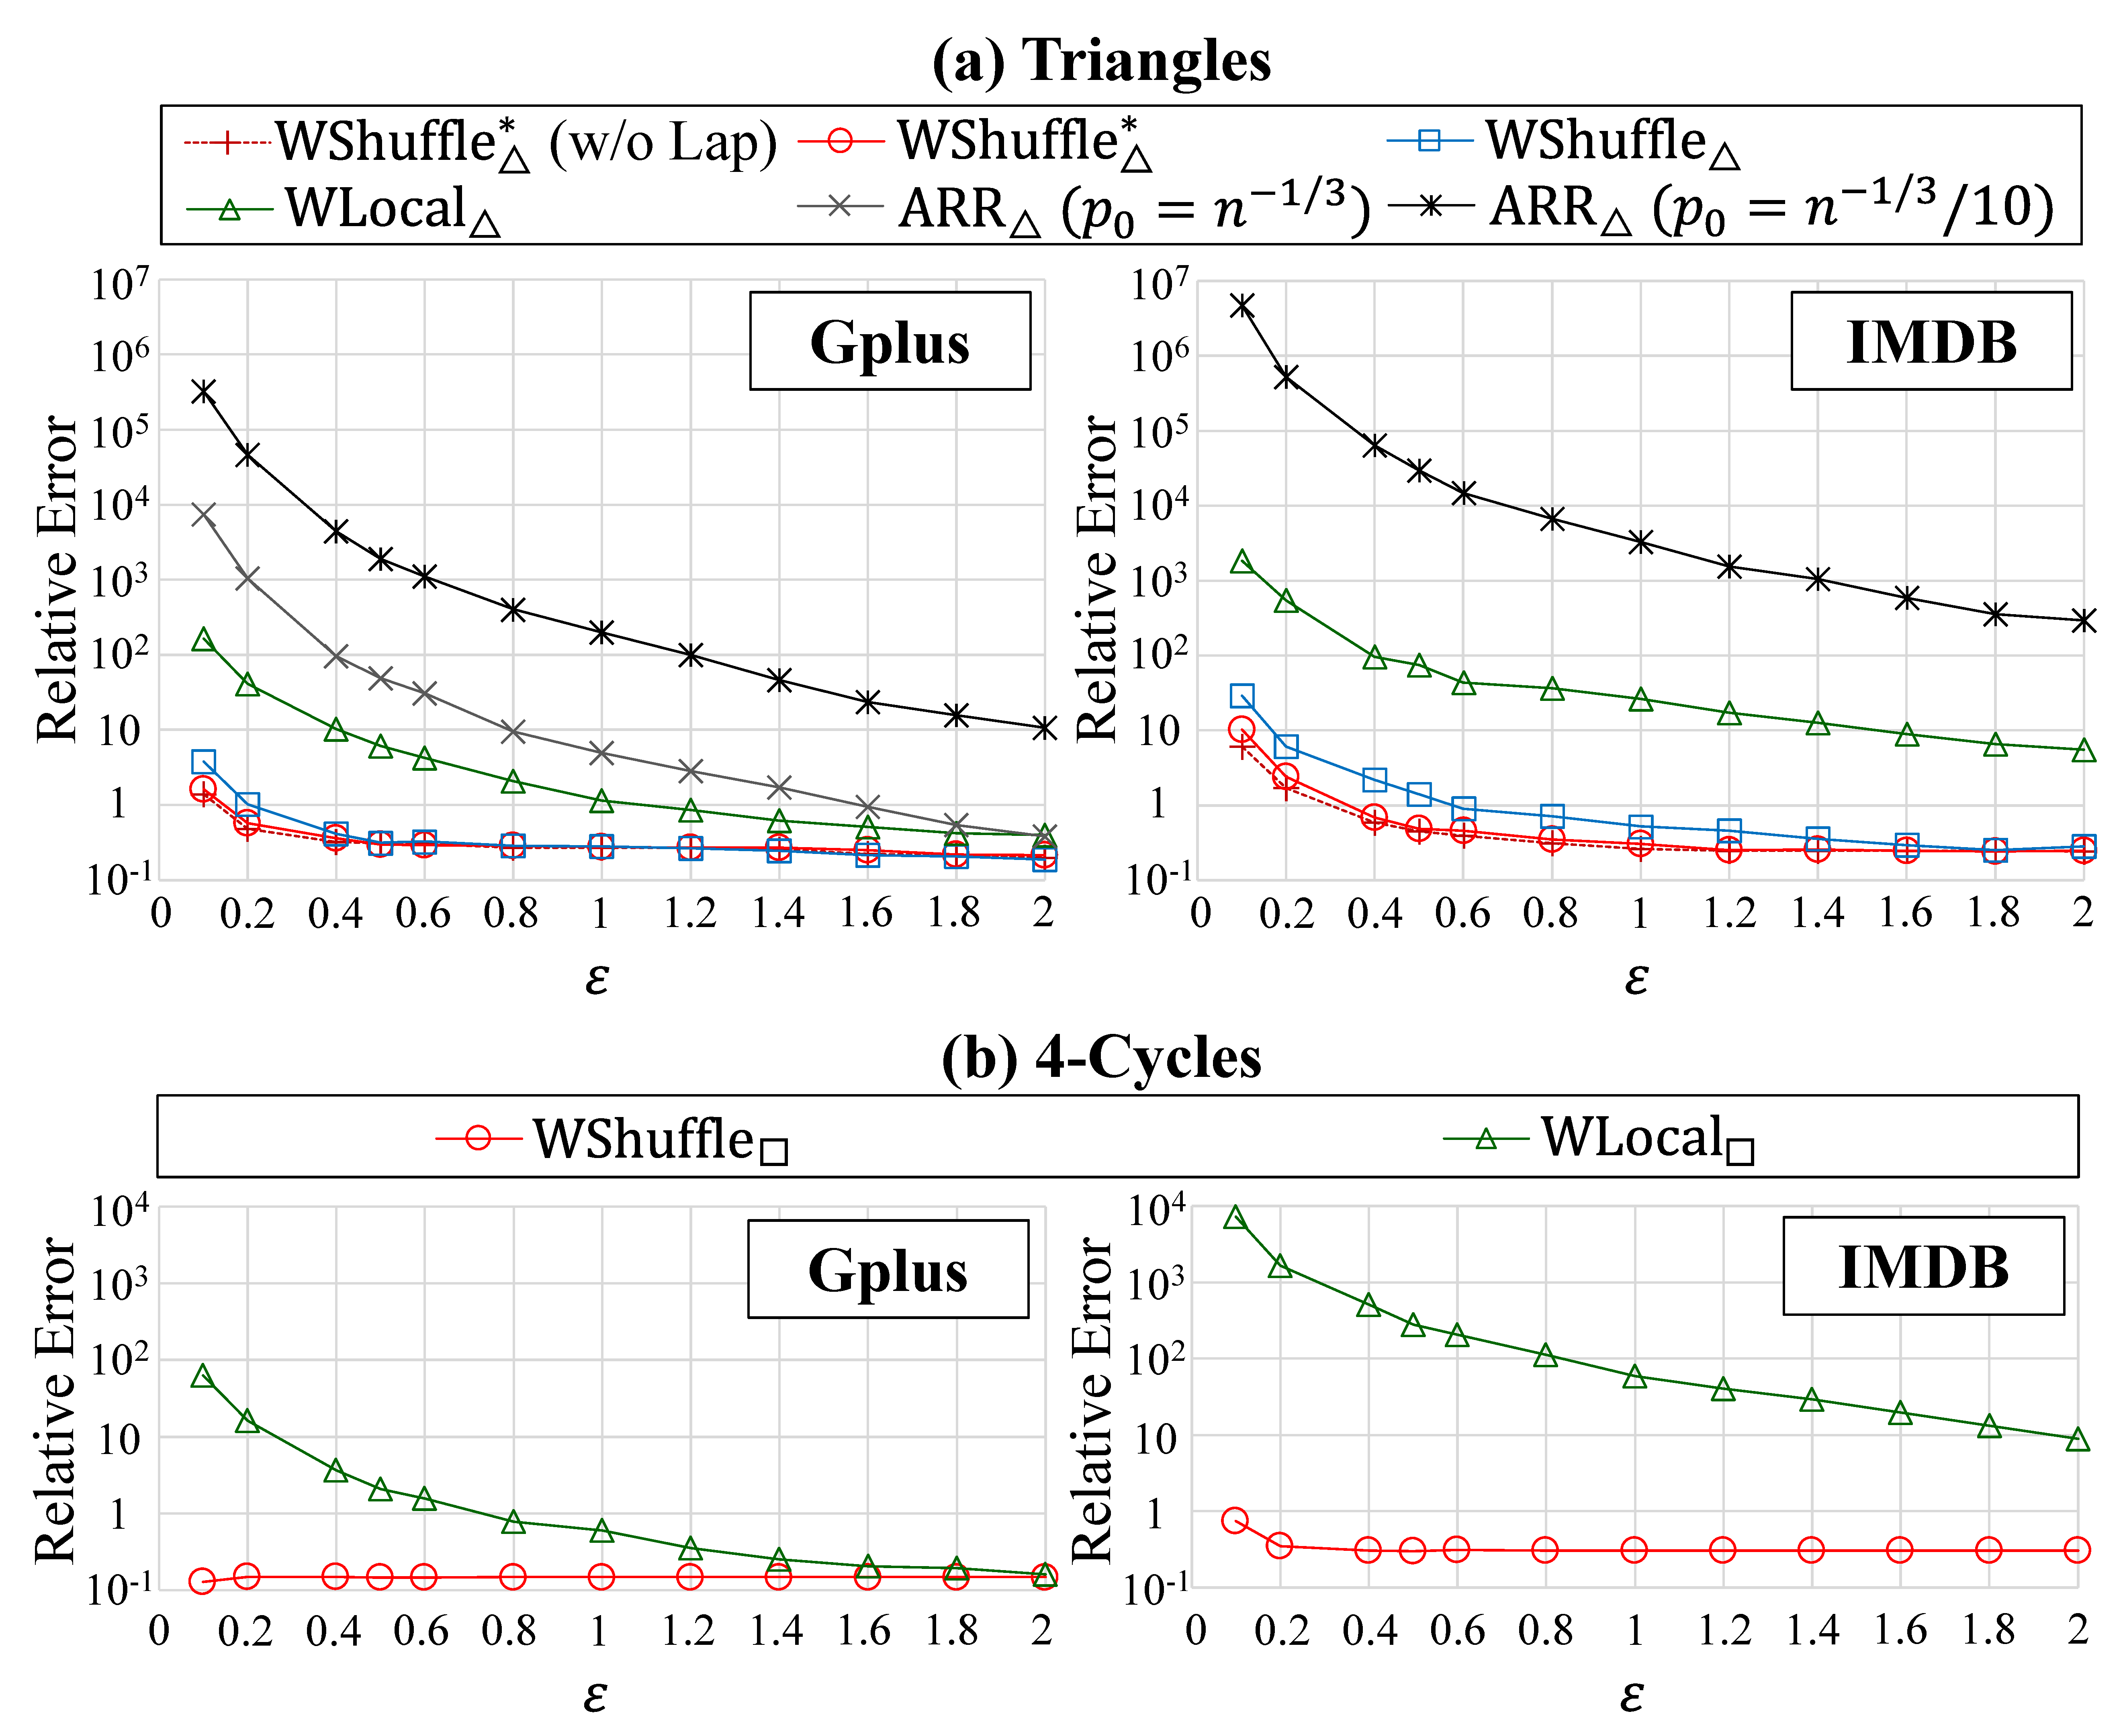
\includegraphics[width=0.99\linewidth]{fig/res1_eps.pdf}
  \vspace{-4mm}
  \caption{Relative error vs. $\epsilon$ 
  %in triangle counting 
  ($n=107614$ in \Gplus{}, $n=896308$ in \IMDB{}, $c=1$). 
  $p_0$ is the sampling probability in the ARR. 
  %; numerical bound in \cite{Feldman_FOCS21}). 
  }
  \label{chap3-fig:res1_eps}
\end{figure}

% \begin{table}[t]
%   \centering
%   (a) \Gplus{}\\
%   \begin{tabular}{|c|c|c|c|}
%     \hline
%     & \AlgWSTriVR{} & \AlgWSTri{} & \AlgWSCyc{} \\ \hline
%     $\epsilon=0.5$ & $0.298$ & $0.312$ & $0.145$ \\ \hline
%     $\epsilon=1$ & $0.277$ & $0.279$ & $0.147$ \\ \hline
%   \end{tabular}\\
%   (b) \IMDB{}\\
%   \begin{tabular}{|c|c|c|c|}
%     \hline
%      & \AlgWSTriVR{} & \AlgWSTri{} & \AlgWSCyc{} \\ \hline
%     $\epsilon=0.5$ & $0.488$ & $1.41$ & XX \\ \hline
%     $\epsilon=1$ & $0.308$ & $0.522$ & XX \\ \hline
%   \end{tabular}
%   \caption{Relative error when $\epsilon=0.5$ or $1$ ($n=107614$ in \Gplus{} and $896308$ in \IMDB{}; $c=1$). 
%   }
%   \label{chap3-tab:res1_eps_tri_0.5}
% \end{table}

\begin{table}[t]
  \caption{Relative error (RE) when $\epsilon=0.5$ or $1$ and computational time ($n=107614$ in \Gplus{}, $n=896308$ in \IMDB{}, $c=1$). 
  The lowest relative error is highlighted in bold.
  }
  \vspace{-4mm}
  \centering
%   (a) Triangle (\Gplus{})\\
  (a) \Gplus{}\\
  \begin{tabular}{|c|c|c|c|}
    \hline
    & RE ($\epsilon=0.5$) & RE ($\epsilon=1$) & Time (sec)\\ \hline
    \AlgWSTriVR{} & $\bm{2.98 \times 10^{-1}}$ & $\bm{2.77 \times 10^{-1}}$ & $3.60 \times 10^1$ \\ \hline
    \AlgWSTri{} & $3.12 \times 10^{-1}$ & $2.79 \times 10^{-1}$ & $3.62 \times 10^1$ \\ \hline
    \AlgWLTri{} & $6.10 \times 10^0$ & $1.14 \times 10^0$ & $5.83 \times 10^1$ \\ \hline
    \AlgARRTri{} ($p_0=n^{-1/3}$) & $4.90 \times 10^1$ & $4.93 \times 10^0$ & $7.15 \times 10^2$ \\ \hline
    \hspace{-0.5mm}\AlgARRTri{} ($p_0=0.1n^{-1/3}$)\hspace{-0.5mm} & $1.88 \times 10^3$ & $1.97 \times 10^2$ & $3.48 \times 10^1$ \\ \hline \hline
    \AlgWSCyc{} & $\bm{1.45 \times 10^{-1}}$ & $\bm{1.47 \times 10^{-1}}$ & $3.47 \times 10^1$ \\ \hline
    \AlgWLCyc{} & $2.08 \times 10^0$ & $5.96 \times 10^{-1}$ & $5.70 \times 10^1$ \\ \hline
  \end{tabular}\\
%   (b) Triangle (\IMDB{})\\
  (b) \IMDB{}\\
  \begin{tabular}{|c|c|c|c|}
    \hline
    & RE ($\epsilon=0.5$) & RE ($\epsilon=1$) & Time (sec)\\ \hline
    \AlgWSTriVR{} & $\bm{4.88 \times 10^{-1}}$ & $\bm{3.08 \times 10^{-1}}$ & $2.39 \times 10^3$ \\ \hline
    \AlgWSTri{} & $1.41 \times 10^0$ & $5.22 \times 10^{-1}$ & $2.40 \times 10^3$ \\ \hline
    \AlgWLTri{} & $7.46 \times 10^1$ & $2.63 \times 10^1$ & $3.96 \times 10^3$ \\ \hline
    \hspace{-0.5mm}\AlgARRTri{} ($p_0=0.1n^{-1/3}$)\hspace{-0.5mm} & $2.98 \times 10^4$ & $3.27 \times 10^3$ & $2.81 \times 10^3$ \\ \hline \hline
    \AlgWSCyc{} & $\bm{3.03 \times 10^{-1}}$ & $\bm{3.08 \times 10^{-1}}$ & $2.29 \times 10^3$ \\ \hline
    \AlgWLCyc{} & $2.82 \times 10^2$ & $5.91 \times 10^1$ & $3.91 \times 10^3$ \\ \hline
  \end{tabular}
%   (c) 4-cycle (\Gplus{})\\
%   \begin{tabular}{|c|c|c|c|}
%     \hline
%     & RE ($\epsilon=0.5$) & RE ($\epsilon=1$) & Time (sec)\\ \hline
%     \AlgWSCyc{} & $XXX$ & $XXX$ & $XXX$ \\ \hline
%     \AlgWLCyc{} & $XXX$ & $XXX$ & $XXX$ \\ \hline
%   \end{tabular}\\
  \label{chap3-tab:res1_eps_tri_time}
\end{table}

Figure~\ref{chap3-fig:res1_eps} shows the relative error ($c=1$). 
% Here, we used the numerical upper bound in \cite{Feldman_FOCS21} for $\epsilon$ in the shuffle algorithms. 
% We also 
Here, we show the performance of \AlgWSTri{} when we do not add the Laplacian noise (denoted by \AlgWSTri{} (w/o Lap)). 
In \IMDB{}, we do not show \AlgARRTri{} with $p_0 = n^{-1/3}$, because it takes too much time (longer than one day). 
Table~\ref{chap3-tab:res1_eps_tri_time} highlights the relative error when $\epsilon=0.5$ or $1$. 
It also shows the running time of counting triangles or 4-cycles when $\epsilon=1$ (we verified that the running time had little dependence on $\epsilon$). 

Figure~\ref{chap3-fig:res1_eps} and Table~\ref{chap3-tab:res1_eps_tri_time} show that our shuffle algorithms dramatically improve the local algorithms. 
% For example, 
In triangle counting, 
\AlgWSTriVR{} outperforms \AlgWLTri{} by one or two orders of magnitude and \AlgARRTri{} by even more\footnote{Note that \AlgARRTri{} uses only the lower-triangular part of the adjacency matrix $\bmA$ and therefore provides 
% $\epsilon$-edge LDP and 
$\epsilon$-edge DP (rather than $2\epsilon$-edge DP); i.e., it does not suffer from the doubling issue explained in Section~\ref{chap3-sub:privacy}. However, Figure~\ref{chap3-fig:res1_eps} shows that \AlgWSTriVR{} significantly outperforms \AlgARRTri{} 
% with the same privacy budget in edge DP.
even if we double $\epsilon$ for only \AlgWSTriVR{}.}. 
% Although the relative error of \AlgARRTri{} can be improved by using a larger $p_0$, it results in longer running time. 
\AlgWSTriVR{} also requires less running time than \AlgARRTri{} with $p_0 = n^{-1/3}$. 
Although the running time of \AlgARRTri{} can be improved by using a smaller $p_0$, it results in a higher relative error. 
% Similarly, 
In 4-cycle counting, 
\AlgWSCyc{} significantly outperforms \AlgWLCyc{}. 
The difference between our shuffle algorithms and the local algorithms is larger in \IMDB{} because it is more sparse; i.e., the difference between $d_{max}$ and $n$ is larger in \IMDB{}. 
This is consistent with our theoretical results in Tables~\ref{chap3-tab:upper_bounds_triangle} and \ref{chap3-tab:upper_bounds_4cycle}. 

Figure~\ref{chap3-fig:res1_eps} and Table~\ref{chap3-tab:res1_eps_tri_time} also show that \AlgWSTriVR{} outperforms \AlgWSTri{}, especially when $\epsilon$ is small. 
% or the dataset is sparse, i.e., \IMDB{}. 
This is because the variance is large when $\epsilon$ is small. 
In addition, \AlgWSTriVR{} significantly outperforms \AlgWSTri{} in \IMDB{} because \AlgWSTriVR{} significantly reduces the variance when $d_{max} \ll n$, as shown in Table~\ref{chap3-tab:upper_bounds_triangle}. 
In other words, this is also consistent with our theoretical results. 
For example, when $\epsilon=0.5$, our variance reduction technique reduces the relative error from $1.41$ to $0.488$ (about one-third) in \IMDB{}. 

Furthermore, Figure~\ref{chap3-fig:res1_eps} shows that the relative error of \AlgWSTriVR{} is hardly changed by adding the Laplacian noise. 
This is because the sensitivity of each user's degree $d_i$ is very small ($=1$). 
In this case, the Laplacian noise is also very small. 

\begin{figure}[t]
  \centering
  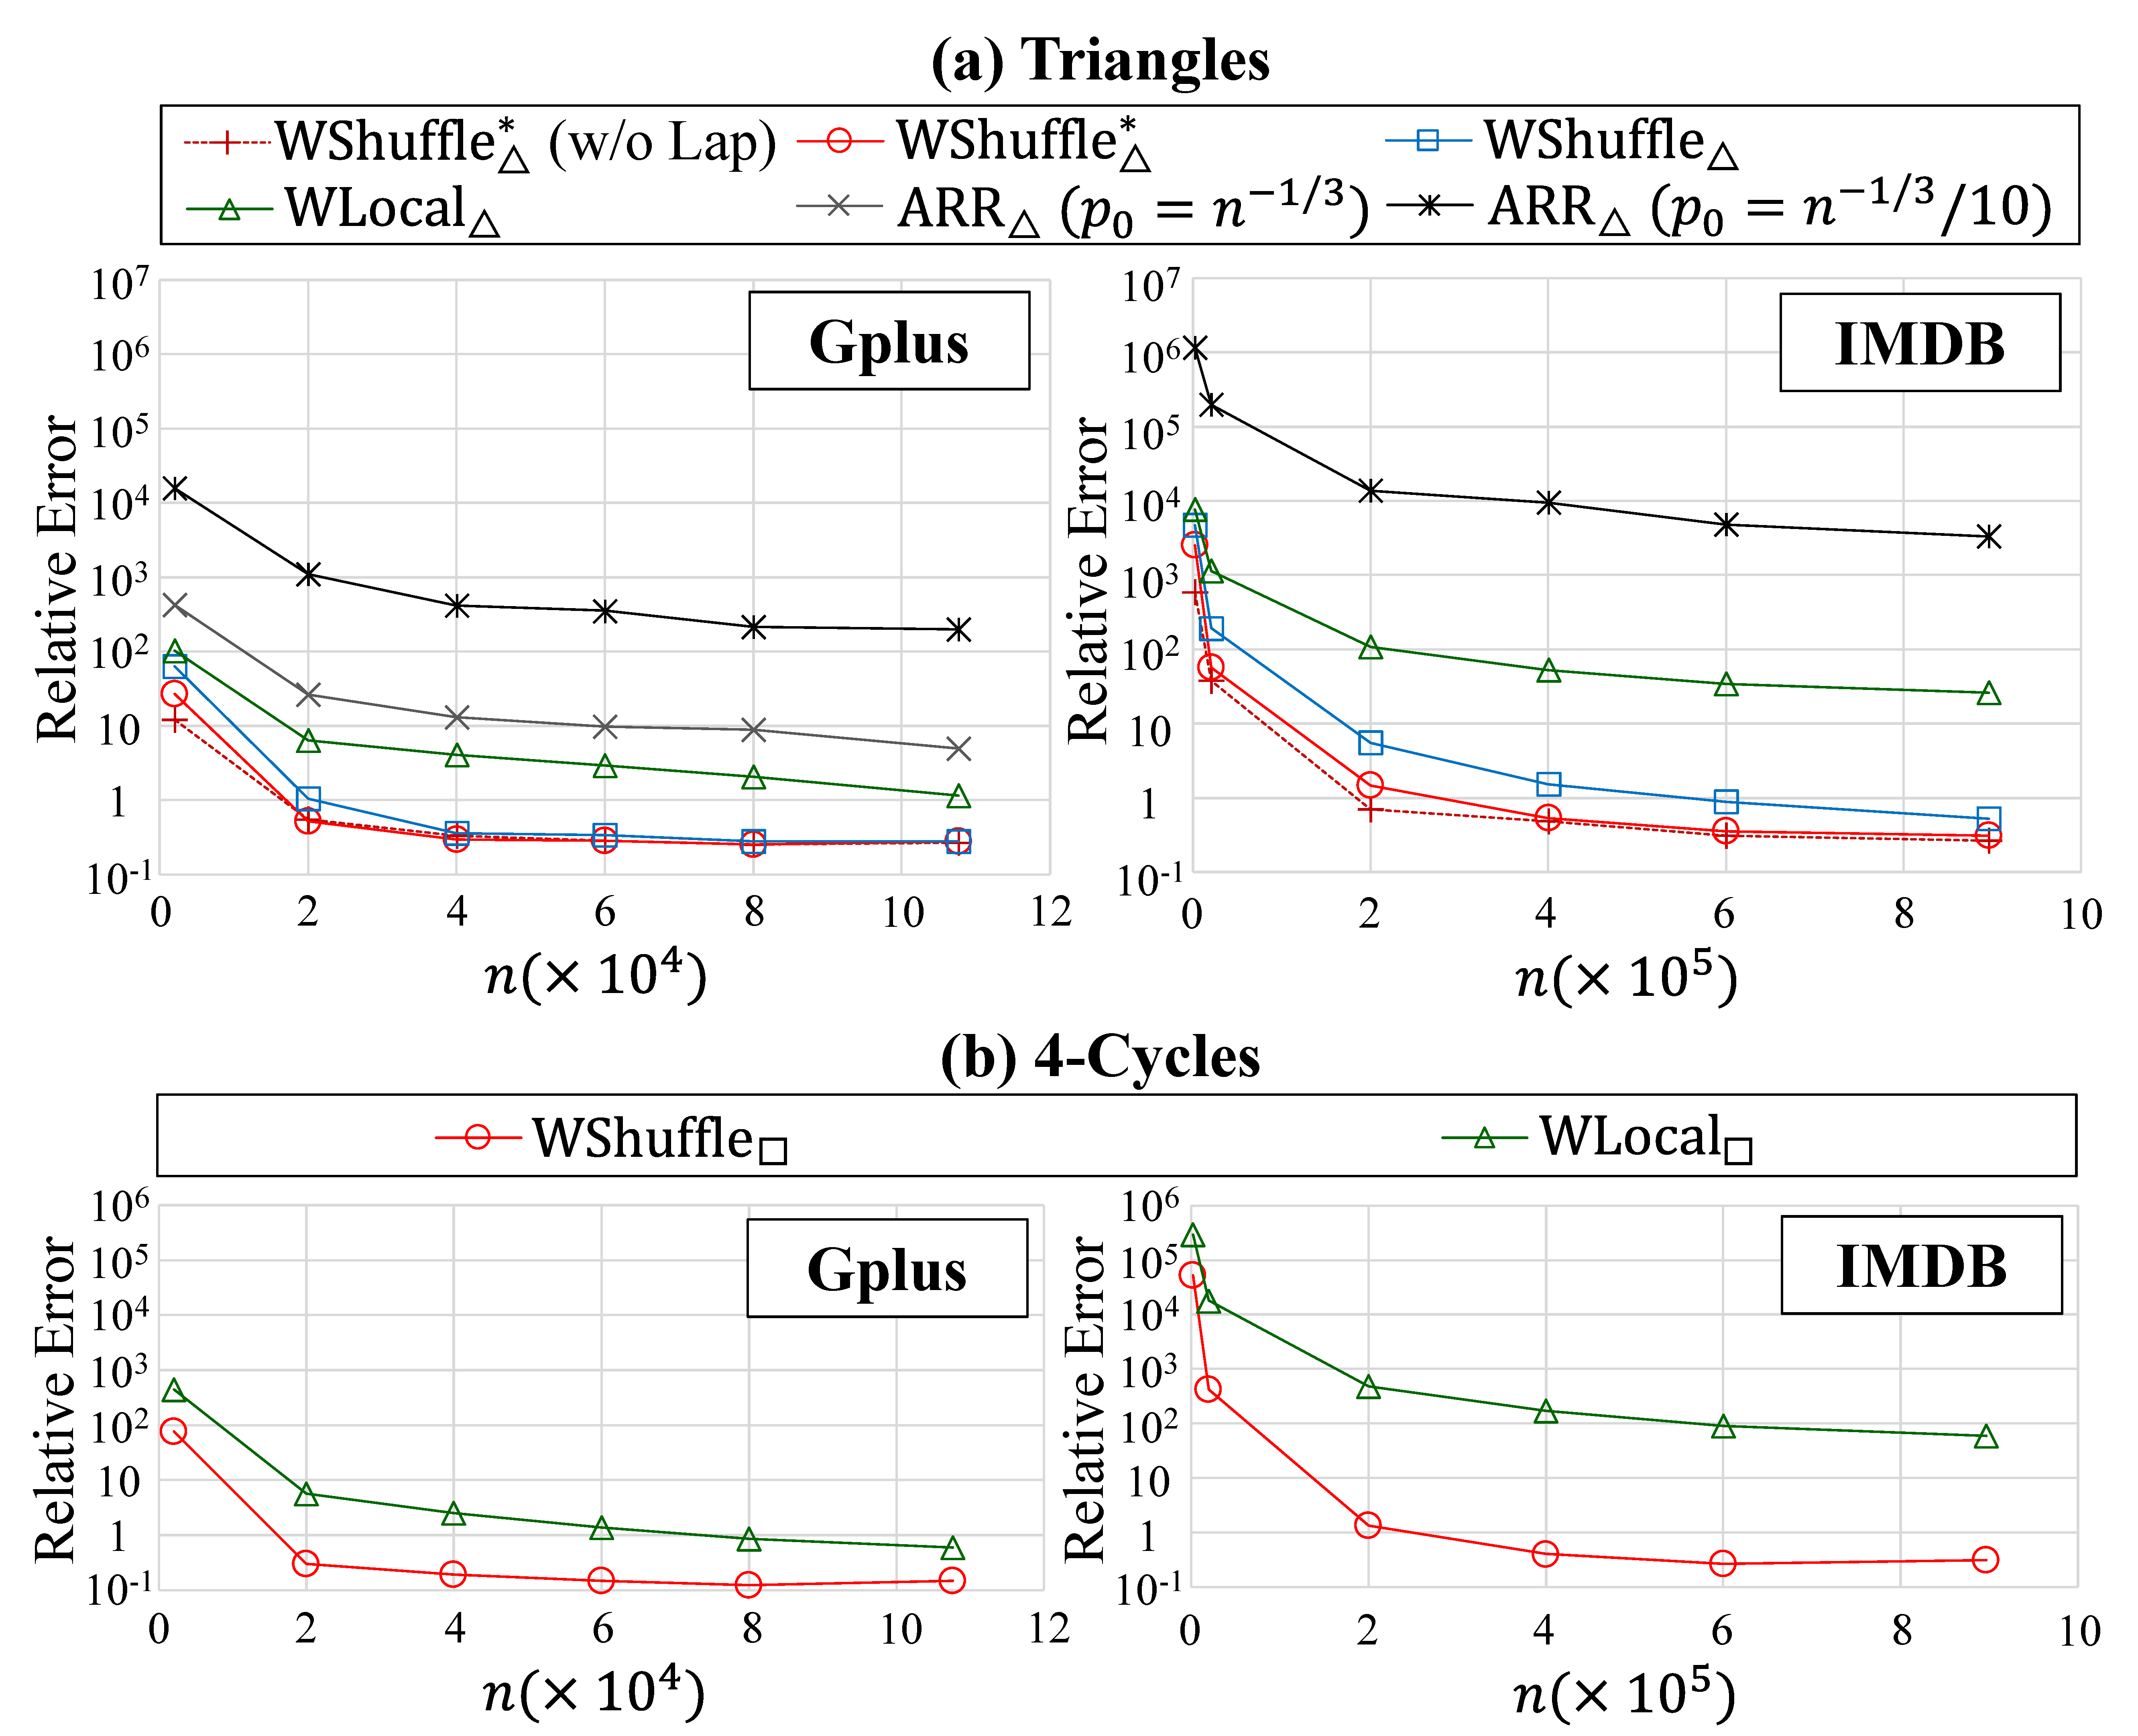
\includegraphics[width=0.99\linewidth]{fig/res2_n.pdf}
  \vspace{-4mm}
  \caption{Relative error vs. $n$ ($\epsilon=1$, $c=1$).
  }
  \label{chap3-fig:res2_n}
\end{figure}

% Table~\ref{chap3-tab:res1_eps_tri_time} shows that 
Our \AlgWSTriVR{} achieves a relative error of $0.3$ ($\ll 1$) 
% and \AlgWSCyc{} achieve relative errors of $0.15$ to $0.3$ ($\ll 1$) 
% with a reasonable privacy budget -- $\epsilon = 0.5$ or $1$ in element DP and $2\epsilon = 1$ or $2$ in edge DP. 
when the privacy budget is $\epsilon = 0.5$ or $1$ in element DP ($2\epsilon = 1$ or $2$ in edge DP). 
\AlgWSCyc{} achieve a relative error of $0.15$ to $0.3$ with a smaller privacy budget (e.g., $\epsilon = 0.2$) because it  does not send local edges -- the error of \AlgWSCyc{} is mainly caused by user-pair sampling that is independent of $\epsilon$. 

In summary, our \AlgWSTriVR{} and \AlgWSCyc{} significantly outperform the local algorithms and achieve a relative error much smaller than $1$ with a reasonable privacy budget, i.e., $\epsilon \leq 1$. 

\smallskip
\noindent{\textbf{Relative Error vs. $n$.}}~~Next, we evaluated the relation between the relative error and $n$. 
% the number $n$ of users. 
Specifically, we randomly selected $n$ users from all users and extracted a graph with $n$ users. 
Then we set $\epsilon = 1$ and changed $n$ to various values starting from $2000$. 
%from $2000$ to $107614$ and $896308$ in \Gplus{} and \IMDB{}, respectively. 

Figure~\ref{chap3-fig:res2_n} shows the results ($c=1$). 
% We observe that 
When $n=2000$, \AlgWSTri{} and \AlgWSCyc{} provide 
%almost the same relative error as 
relative errors close to \AlgWLTri{} and \AlgWLCyc{}, respectively. 
This is because the privacy amplification effect is limited when $n$ is small. 
For example, when $n=2000$ and $\epsilon=1$, 
% and $\delta=10^{-8}$, 
the numerical bound is $\epsilon_L=1.88$. 
The value of $\epsilon_L$ increases with increase in $n$; e.g., when $n=107614$ and $896308$, the numerical bound is $\epsilon_L= 5.86$ and $7.98$, respectively. 
This explains the reason that our shuffle algorithms significantly outperform the local algorithms when $n$ is large in Figure~\ref{chap3-fig:res2_n}. 
% the large difference between our shuffle algorithms and the local algorithms. 
% in Figure~XX. 

% Figure~XX also shows that the relative error decreases with increase in $n$. 
% There are two reasons for this: (i) the squares of the true triangle and 4-cycle counts are $O(n^2 d_{max}^4)$ and $O(n^2 d_{max}^6)$, respectively; (ii) $d_{max}$ is proportional to $n$, as we randomly selected $n$ users from all users. 


% \smallskip
% \noindent{\textbf{Clustering Coefficient.}}~~TBD

\smallskip
\noindent{\textbf{Parameter $c$ in \AlgWSTriVR{}.}}~~Finally, we evaluated our \AlgWSTriVR{} while changing the parameter $c$ that controls the bias and variance. 
% of the estimate. 
Recall that as $c$ increases, the bias is increased, and the variance is reduced. 
We set $\epsilon=0.1$ or $1$ and changed $c$ from $0.1$ to $4$. 

Figure~\ref{chap3-fig:res4_thr} shows the results. 
Here, we also show the relative error of \AlgWSTri{}. 
We observe that the optimal $c$ is different for $\epsilon=0.1$ and $\epsilon=1$. The optimal $c$ is around $3$ to $4$ for $\epsilon=0.1$, whereas the optimal $c$ is around $0.5$ to $1$ for $\epsilon=1$. 
This is because the variance of \AlgWSTri{} is large (resp.~small) when $\epsilon$ is small (resp.~large). 
For a small $\epsilon$, a large $c$ is effective in significantly reducing the variance. 
For a large $\epsilon$, a small $c$ is effective in keeping a small bias. 
% The optimization of $c$ in \AlgWSTriVR{} is an interesting future research direction. 

We also observe that \AlgWSTriVR{} is always better than (or almost the same as) \AlgWSTri{} when $c=1$ or $2$. 
This is because most users' degrees are smaller than the average degree $d_{avg}$, as described in Section~\ref{chap3-sub:var_red}. 
When $c=1$ or $2$, most user-pairs are ignored. 
Therefore, we can significantly reduce the variance at the cost of a small bias. 

\begin{figure}[t]
  \centering
  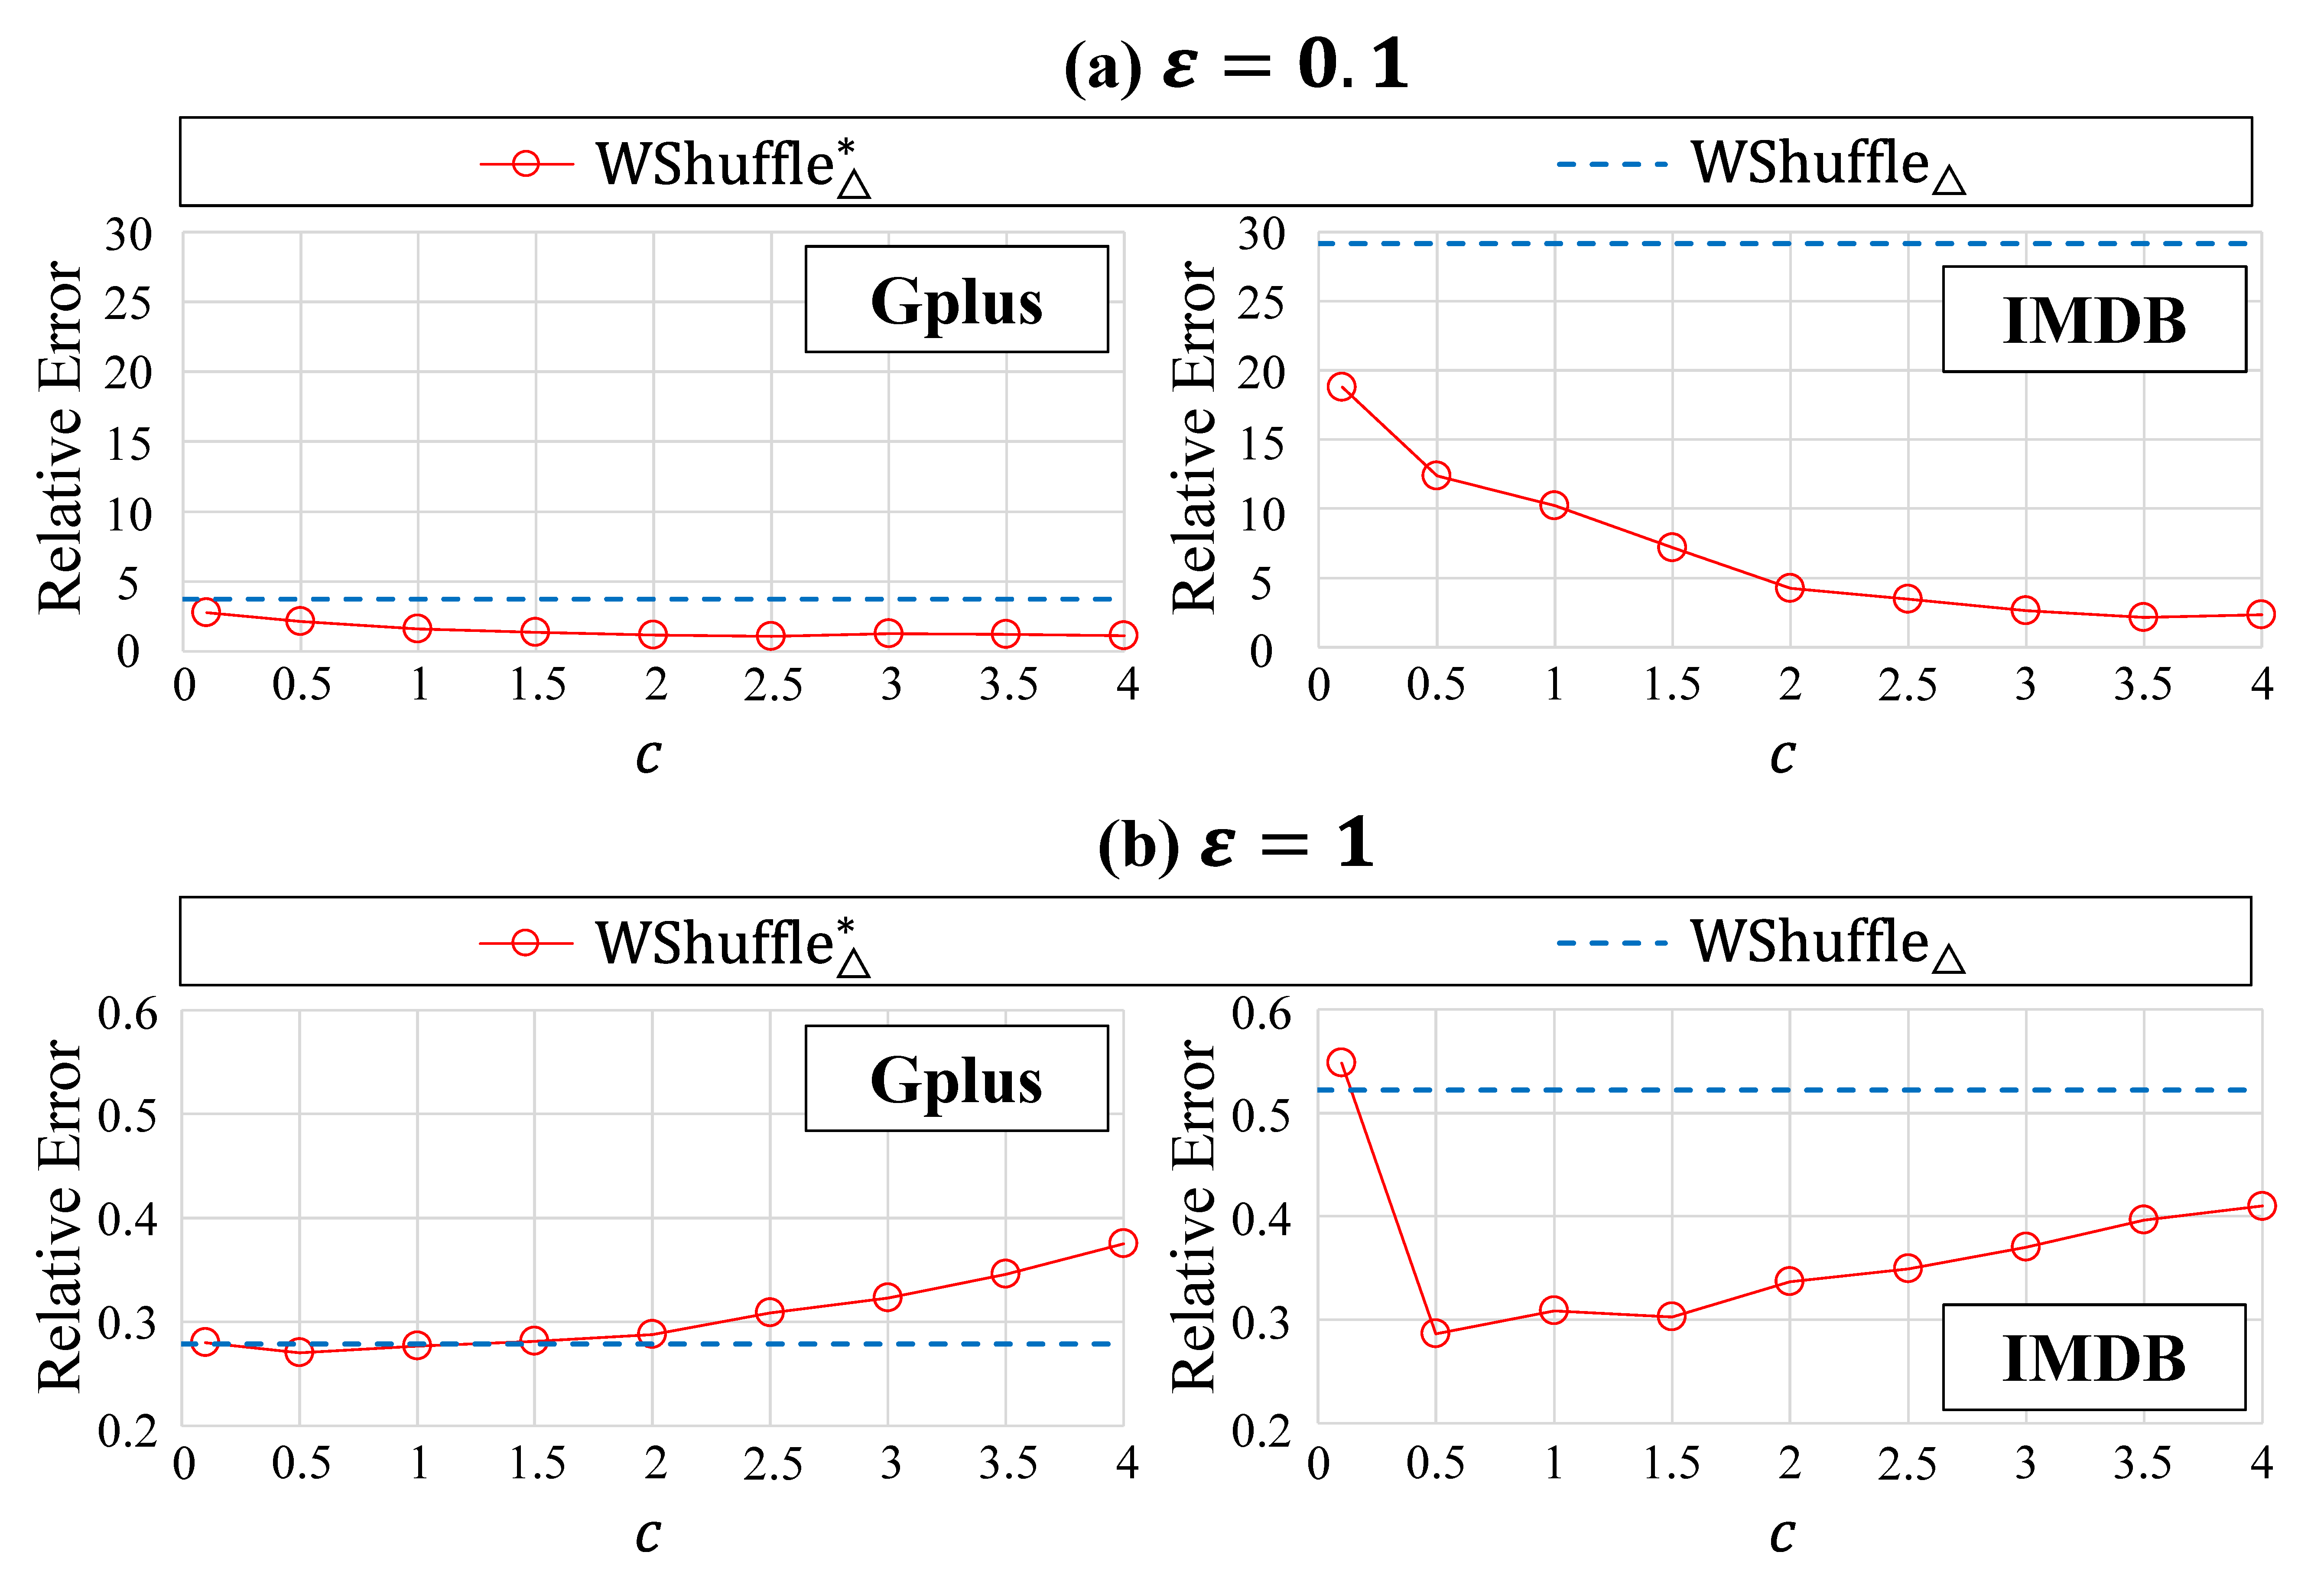
\includegraphics[width=0.99\linewidth]{fig/res4_thr.pdf}
  \vspace{-4mm}
  \caption{Relative error vs. parameter $c$ in \AlgWSTriVR{} ($n=107614$ in \Gplus{}, $n=896308$ in \IMDB{}).
  }
  \label{chap3-fig:res4_thr}
\end{figure}

\smallskip
\noindent{\textbf{Summary.}}~~In summary, our answers to the three questions at the beginning of Section~\ref{chap3-sec:experiments} are as follows. 
RQ1: Our \AlgWSTriVR{} and \AlgWSCyc{} outperform the one-round local algorithms by one or two orders of magnitude (or even more). 
% \AlgWSTriVR{} is even comparable to the two-rounds local algorithm in \cite{Imola_USENIX22} (\AlgTwoRS{}) that requires a lot of user effort 
% and synchronization 
% in terms of accuracy. 
RQ2: Our variance reduction technique significantly reduces the relative error (e.g., by about one-third) 
for a small $\epsilon$ in a sparse dataset. 
% when $\epsilon$ is small or the dataset is sparse. 
RQ3: 
% Our \AlgWSTriVR{} and \AlgWSCyc{} achieve a relative error of $0.15$ to $0.3$ ($\ll 1$) when $\epsilon=0.5$ or $1$ in element DP ($2\epsilon=1$ or $2$ in edge DP). 
\AlgWSTriVR{} achieves a relative error of $0.3$ ($\ll 1$) when $\epsilon=0.5$ or $1$ in element DP ($2\epsilon=1$ or $2$ in edge DP). 
\AlgWSCyc{} achieves a relative error of $0.15$ to $0.3$ with a smaller privacy budget: $\epsilon=0.2$. 

\section{Conclusion}
\label{chap3-sec:conclusion}
In this paper, we made the first attempt (to our knowledge) to 
shuffle graph data for privacy amplification. 
% apply the shuffle model to graph data. 
We proposed wedge shuffling as a basic technique and then applied it to 
% to enable the privacy amplification of graph data. 
% Then we proposed 
one-round triangle and 4-cycle counting with several additional techniques. 
% algorithms based on wedge shuffling. 
We showed upper bounds on 
% the expected $l_2$ loss 
the MSE 
for each algorithm. 
We also showed through comprehensive experiments that our one-round shuffle algorithms significantly outperform the one-round local algorithms and achieve a small relative error with a reasonable privacy budget, e.g., smaller than $1$ in edge DP. 

For future work, we would like to apply wedge shuffling to other subgraphs such as 3-hop paths \cite{Sun_CCS19} and $k$-triangles \cite{Karwa_PVLDB11}. 




\appendix
%\Blinddocument

% Stuff at the end of the dissertation goes in the back matter
\backmatter
\bibliographystyle{plain} % Or whatever style you want like plainnat
\bibliography{references}

\end{document}
